% Created by tikzDevice version 0.12.3.1 on 2023-07-02 20:59:36
% !TEX encoding = UTF-8 Unicode
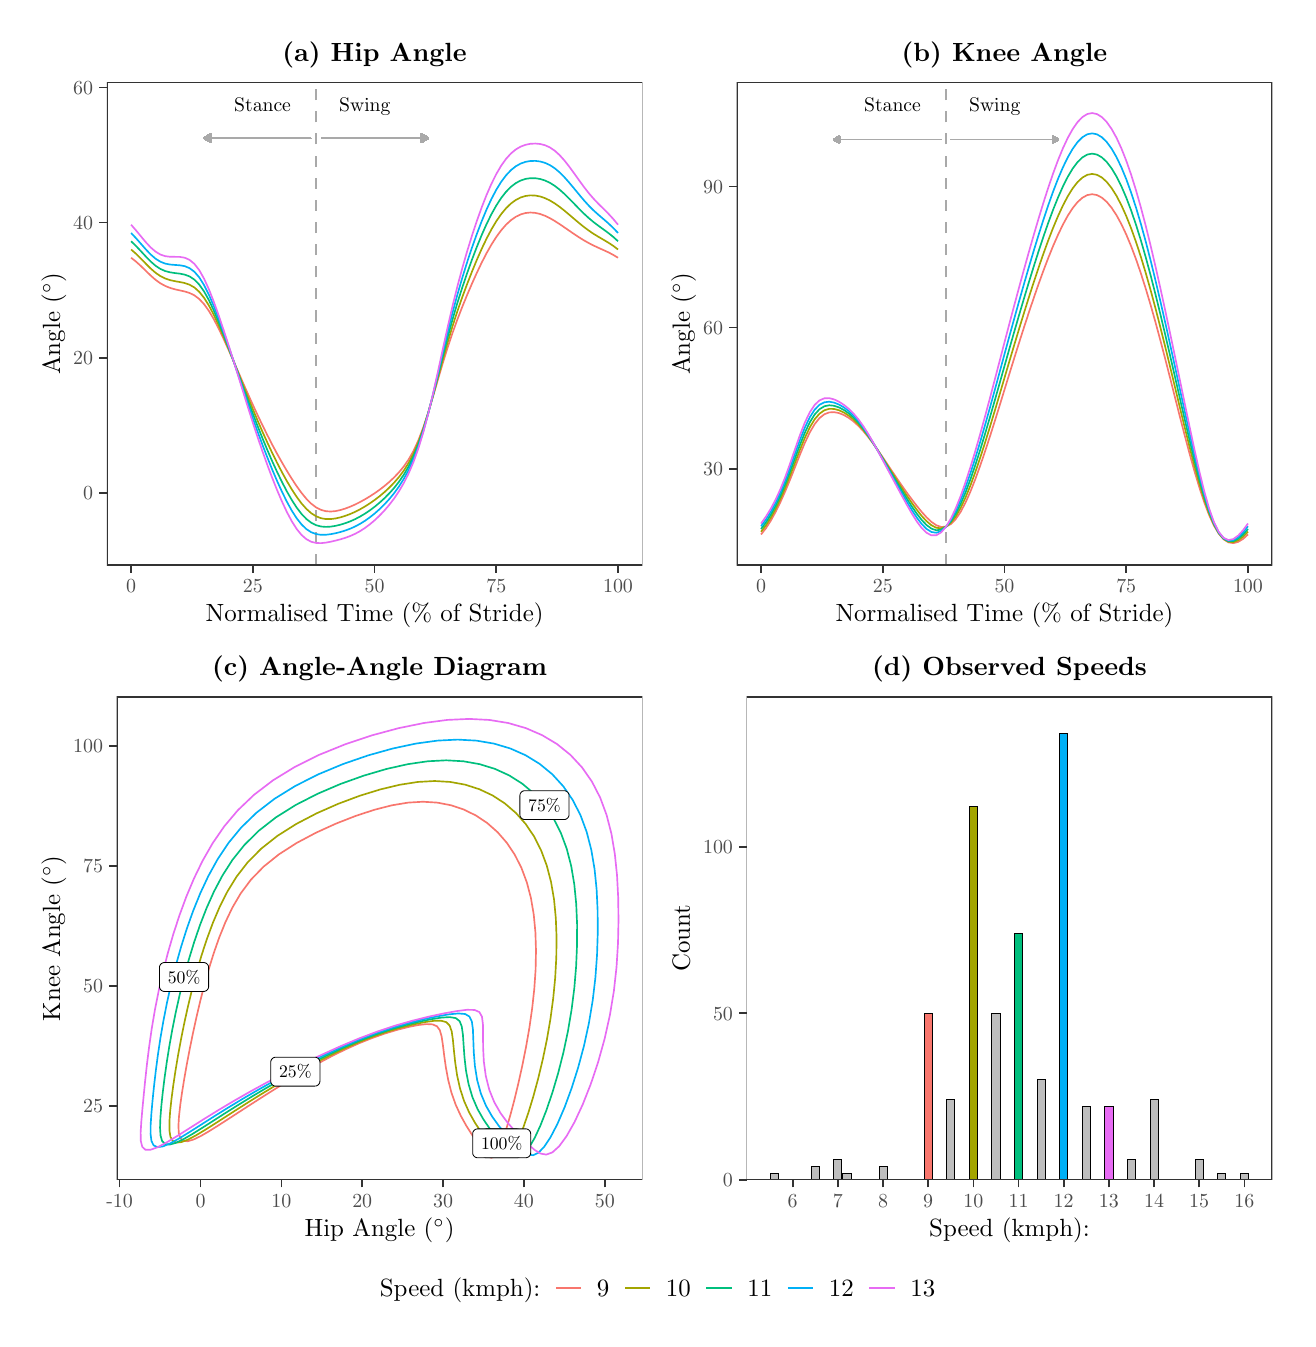
\begin{tikzpicture}[x=1pt,y=1pt]
\definecolor{fillColor}{RGB}{255,255,255}
\path[use as bounding box,fill=fillColor,fill opacity=0.00] (0,0) rectangle (455.24,466.62);
\begin{scope}
\path[clip] (  0.00,244.53) rectangle (227.62,466.62);
\definecolor{drawColor}{RGB}{255,255,255}
\definecolor{fillColor}{RGB}{255,255,255}

\path[draw=drawColor,line width= 0.6pt,line join=round,line cap=round,fill=fillColor] ( -0.00,244.53) rectangle (227.62,466.62);
\end{scope}
\begin{scope}
\path[clip] ( 28.58,272.42) rectangle (222.12,446.86);
\definecolor{fillColor}{RGB}{255,255,255}

\path[fill=fillColor] ( 28.58,272.42) rectangle (222.12,446.86);
\definecolor{drawColor}{RGB}{169,169,169}

\path[draw=drawColor,line width= 0.9pt,dash pattern=on 4pt off 4pt ,line join=round] (104.24,272.42) -- (104.24,446.86);
\definecolor{drawColor}{RGB}{248,118,109}

\path[draw=drawColor,line width= 0.6pt,line join=round] ( 37.38,383.48) --
	( 39.14,382.09) --
	( 40.90,380.50) --
	( 42.66,378.78) --
	( 44.42,377.07) --
	( 46.18,375.52) --
	( 47.94,374.25) --
	( 49.70,373.29) --
	( 51.46,372.58) --
	( 53.22,372.07) --
	( 54.98,371.68) --
	( 56.74,371.29) --
	( 58.49,370.75) --
	( 60.25,369.89) --
	( 62.01,368.55) --
	( 63.77,366.66) --
	( 65.53,364.20) --
	( 67.29,361.23) --
	( 69.05,357.83) --
	( 70.81,354.14) --
	( 72.57,350.25) --
	( 74.33,346.25) --
	( 76.09,342.22) --
	( 77.85,338.20) --
	( 79.61,334.22) --
	( 81.37,330.33) --
	( 83.13,326.53) --
	( 84.89,322.86) --
	( 86.65,319.30) --
	( 88.40,315.88) --
	( 90.16,312.60) --
	( 91.92,309.46) --
	( 93.68,306.45) --
	( 95.44,303.60) --
	( 97.20,300.94) --
	( 98.96,298.50) --
	(100.72,296.36) --
	(102.48,294.60) --
	(104.24,293.26) --
	(106.00,292.37) --
	(107.76,291.89) --
	(109.52,291.78) --
	(111.28,291.94) --
	(113.04,292.32) --
	(114.80,292.86) --
	(116.56,293.53) --
	(118.32,294.31) --
	(120.07,295.19) --
	(121.83,296.16) --
	(123.59,297.22) --
	(125.35,298.36) --
	(127.11,299.60) --
	(128.87,300.95) --
	(130.63,302.44) --
	(132.39,304.09) --
	(134.15,305.94) --
	(135.91,308.07) --
	(137.67,310.60) --
	(139.43,313.70) --
	(141.19,317.53) --
	(142.95,322.16) --
	(144.71,327.50) --
	(146.47,333.34) --
	(148.23,339.39) --
	(149.98,345.34) --
	(151.74,351.00) --
	(153.50,356.26) --
	(155.26,361.14) --
	(157.02,365.69) --
	(158.78,370.00) --
	(160.54,374.11) --
	(162.30,378.03) --
	(164.06,381.71) --
	(165.82,385.13) --
	(167.58,388.23) --
	(169.34,391.00) --
	(171.10,393.40) --
	(172.86,395.42) --
	(174.62,397.04) --
	(176.38,398.28) --
	(178.14,399.14) --
	(179.90,399.64) --
	(181.65,399.82) --
	(183.41,399.69) --
	(185.17,399.29) --
	(186.93,398.64) --
	(188.69,397.79) --
	(190.45,396.77) --
	(192.21,395.63) --
	(193.97,394.44) --
	(195.73,393.22) --
	(197.49,392.02) --
	(199.25,390.85) --
	(201.01,389.76) --
	(202.77,388.77) --
	(204.53,387.87) --
	(206.29,387.05) --
	(208.05,386.26) --
	(209.81,385.45) --
	(211.57,384.53) --
	(213.32,383.47);
\definecolor{drawColor}{RGB}{163,165,0}

\path[draw=drawColor,line width= 0.6pt,line join=round] ( 37.38,386.46) --
	( 39.14,384.91) --
	( 40.90,383.19) --
	( 42.66,381.37) --
	( 44.42,379.61) --
	( 46.18,378.07) --
	( 47.94,376.85) --
	( 49.70,375.98) --
	( 51.46,375.39) --
	( 53.22,375.01) --
	( 54.98,374.70) --
	( 56.74,374.34) --
	( 58.49,373.74) --
	( 60.25,372.73) --
	( 62.01,371.15) --
	( 63.77,368.95) --
	( 65.53,366.14) --
	( 67.29,362.79) --
	( 69.05,359.01) --
	( 70.81,354.94) --
	( 72.57,350.67) --
	( 74.33,346.29) --
	( 76.09,341.85) --
	( 77.85,337.41) --
	( 79.61,333.01) --
	( 81.37,328.71) --
	( 83.13,324.53) --
	( 84.89,320.49) --
	( 86.65,316.60) --
	( 88.40,312.87) --
	( 90.16,309.31) --
	( 91.92,305.92) --
	( 93.68,302.73) --
	( 95.44,299.77) --
	( 97.20,297.07) --
	( 98.96,294.70) --
	(100.72,292.72) --
	(102.48,291.16) --
	(104.24,290.05) --
	(106.00,289.36) --
	(107.76,289.05) --
	(109.52,289.05) --
	(111.28,289.28) --
	(113.04,289.68) --
	(114.80,290.22) --
	(116.56,290.88) --
	(118.32,291.66) --
	(120.07,292.56) --
	(121.83,293.57) --
	(123.59,294.69) --
	(125.35,295.92) --
	(127.11,297.26) --
	(128.87,298.74) --
	(130.63,300.37) --
	(132.39,302.18) --
	(134.15,304.22) --
	(135.91,306.57) --
	(137.67,309.34) --
	(139.43,312.71) --
	(141.19,316.80) --
	(142.95,321.71) --
	(144.71,327.37) --
	(146.47,333.59) --
	(148.23,340.10) --
	(149.98,346.59) --
	(151.74,352.83) --
	(153.50,358.69) --
	(155.26,364.12) --
	(157.02,369.18) --
	(158.78,373.93) --
	(160.54,378.44) --
	(162.30,382.71) --
	(164.06,386.70) --
	(165.82,390.39) --
	(167.58,393.73) --
	(169.34,396.69) --
	(171.10,399.24) --
	(172.86,401.36) --
	(174.62,403.07) --
	(176.38,404.36) --
	(178.14,405.26) --
	(179.90,405.80) --
	(181.65,406.02) --
	(183.41,405.95) --
	(185.17,405.62) --
	(186.93,405.02) --
	(188.69,404.18) --
	(190.45,403.12) --
	(192.21,401.87) --
	(193.97,400.48) --
	(195.73,399.00) --
	(197.49,397.50) --
	(199.25,396.01) --
	(201.01,394.59) --
	(202.77,393.28) --
	(204.53,392.09) --
	(206.29,391.02) --
	(208.05,389.99) --
	(209.81,388.94) --
	(211.57,387.78) --
	(213.32,386.46);
\definecolor{drawColor}{RGB}{0,191,125}

\path[draw=drawColor,line width= 0.6pt,line join=round] ( 37.38,389.44) --
	( 39.14,387.73) --
	( 40.90,385.87) --
	( 42.66,383.96) --
	( 44.42,382.15) --
	( 46.18,380.61) --
	( 47.94,379.45) --
	( 49.70,378.67) --
	( 51.46,378.21) --
	( 53.22,377.94) --
	( 54.98,377.73) --
	( 56.74,377.39) --
	( 58.49,376.73) --
	( 60.25,375.57) --
	( 62.01,373.76) --
	( 63.77,371.25) --
	( 65.53,368.08) --
	( 67.29,364.35) --
	( 69.05,360.20) --
	( 70.81,355.75) --
	( 72.57,351.10) --
	( 74.33,346.33) --
	( 76.09,341.48) --
	( 77.85,336.62) --
	( 79.61,331.81) --
	( 81.37,327.10) --
	( 83.13,322.53) --
	( 84.89,318.13) --
	( 86.65,313.90) --
	( 88.40,309.86) --
	( 90.16,306.02) --
	( 91.92,302.39) --
	( 93.68,299.01) --
	( 95.44,295.93) --
	( 97.20,293.21) --
	( 98.96,290.90) --
	(100.72,289.07) --
	(102.48,287.72) --
	(104.24,286.83) --
	(106.00,286.36) --
	(107.76,286.22) --
	(109.52,286.32) --
	(111.28,286.61) --
	(113.04,287.03) --
	(114.80,287.57) --
	(116.56,288.23) --
	(118.32,289.02) --
	(120.07,289.93) --
	(121.83,290.98) --
	(123.59,292.16) --
	(125.35,293.48) --
	(127.11,294.93) --
	(128.87,296.53) --
	(130.63,298.30) --
	(132.39,300.27) --
	(134.15,302.51) --
	(135.91,305.07) --
	(137.67,308.09) --
	(139.43,311.71) --
	(141.19,316.08) --
	(142.95,321.26) --
	(144.71,327.24) --
	(146.47,333.84) --
	(148.23,340.81) --
	(149.98,347.84) --
	(151.74,354.67) --
	(153.50,361.11) --
	(155.26,367.10) --
	(157.02,372.66) --
	(158.78,377.87) --
	(160.54,382.77) --
	(162.30,387.39) --
	(164.06,391.69) --
	(165.82,395.65) --
	(167.58,399.22) --
	(169.34,402.37) --
	(171.10,405.07) --
	(172.86,407.31) --
	(174.62,409.10) --
	(176.38,410.45) --
	(178.14,411.39) --
	(179.90,411.97) --
	(181.65,412.23) --
	(183.41,412.22) --
	(185.17,411.94) --
	(186.93,411.39) --
	(188.69,410.57) --
	(190.45,409.46) --
	(192.21,408.10) --
	(193.97,406.52) --
	(195.73,404.79) --
	(197.49,402.98) --
	(199.25,401.16) --
	(201.01,399.41) --
	(202.77,397.79) --
	(204.53,396.32) --
	(206.29,394.99) --
	(208.05,393.73) --
	(209.81,392.43) --
	(211.57,391.03) --
	(213.32,389.44);
\definecolor{drawColor}{RGB}{0,176,246}

\path[draw=drawColor,line width= 0.6pt,line join=round] ( 37.38,392.42) --
	( 39.14,390.55) --
	( 40.90,388.55) --
	( 42.66,386.54) --
	( 44.42,384.69) --
	( 46.18,383.16) --
	( 47.94,382.05) --
	( 49.70,381.36) --
	( 51.46,381.02) --
	( 53.22,380.88) --
	( 54.98,380.75) --
	( 56.74,380.44) --
	( 58.49,379.72) --
	( 60.25,378.41) --
	( 62.01,376.37) --
	( 63.77,373.55) --
	( 65.53,370.02) --
	( 67.29,365.91) --
	( 69.05,361.38) --
	( 70.81,356.55) --
	( 72.57,351.53) --
	( 74.33,346.36) --
	( 76.09,341.11) --
	( 77.85,335.83) --
	( 79.61,330.60) --
	( 81.37,325.48) --
	( 83.13,320.52) --
	( 84.89,315.76) --
	( 86.65,311.20) --
	( 88.40,306.85) --
	( 90.16,302.73) --
	( 91.92,298.86) --
	( 93.68,295.29) --
	( 95.44,292.09) --
	( 97.20,289.34) --
	( 98.96,287.11) --
	(100.72,285.42) --
	(102.48,284.28) --
	(104.24,283.62) --
	(106.00,283.36) --
	(107.76,283.38) --
	(109.52,283.60) --
	(111.28,283.94) --
	(113.04,284.38) --
	(114.80,284.93) --
	(116.56,285.58) --
	(118.32,286.37) --
	(120.07,287.30) --
	(121.83,288.39) --
	(123.59,289.64) --
	(125.35,291.03) --
	(127.11,292.59) --
	(128.87,294.31) --
	(130.63,296.23) --
	(132.39,298.37) --
	(134.15,300.79) --
	(135.91,303.58) --
	(137.67,306.84) --
	(139.43,310.72) --
	(141.19,315.35) --
	(142.95,320.82) --
	(144.71,327.11) --
	(146.47,334.09) --
	(148.23,341.52) --
	(149.98,349.09) --
	(151.74,356.50) --
	(153.50,363.53) --
	(155.26,370.08) --
	(157.02,376.15) --
	(158.78,381.81) --
	(160.54,387.11) --
	(162.30,392.07) --
	(164.06,396.69) --
	(165.82,400.92) --
	(167.58,404.72) --
	(169.34,408.06) --
	(171.10,410.91) --
	(172.86,413.26) --
	(174.62,415.13) --
	(176.38,416.53) --
	(178.14,417.51) --
	(179.90,418.13) --
	(181.65,418.44) --
	(183.41,418.48) --
	(185.17,418.26) --
	(186.93,417.77) --
	(188.69,416.96) --
	(190.45,415.81) --
	(192.21,414.33) --
	(193.97,412.56) --
	(195.73,410.57) --
	(197.49,408.46) --
	(199.25,406.32) --
	(201.01,404.23) --
	(202.77,402.29) --
	(204.53,400.54) --
	(206.29,398.96) --
	(208.05,397.46) --
	(209.81,395.93) --
	(211.57,394.27) --
	(213.32,392.43);
\definecolor{drawColor}{RGB}{231,107,243}

\path[draw=drawColor,line width= 0.6pt,line join=round] ( 37.38,395.40) --
	( 39.14,393.37) --
	( 40.90,391.24) --
	( 42.66,389.13) --
	( 44.42,387.23) --
	( 46.18,385.71) --
	( 47.94,384.65) --
	( 49.70,384.05) --
	( 51.46,383.83) --
	( 53.22,383.81) --
	( 54.98,383.78) --
	( 56.74,383.49) --
	( 58.49,382.72) --
	( 60.25,381.25) --
	( 62.01,378.98) --
	( 63.77,375.85) --
	( 65.53,371.97) --
	( 67.29,367.48) --
	( 69.05,362.56) --
	( 70.81,357.36) --
	( 72.57,351.96) --
	( 74.33,346.40) --
	( 76.09,340.74) --
	( 77.85,335.04) --
	( 79.61,329.39) --
	( 81.37,323.86) --
	( 83.13,318.52) --
	( 84.89,313.39) --
	( 86.65,308.50) --
	( 88.40,303.84) --
	( 90.16,299.43) --
	( 91.92,295.32) --
	( 93.68,291.57) --
	( 95.44,288.25) --
	( 97.20,285.48) --
	( 98.96,283.31) --
	(100.72,281.78) --
	(102.48,280.84) --
	(104.24,280.41) --
	(106.00,280.35) --
	(107.76,280.54) --
	(109.52,280.87) --
	(111.28,281.28) --
	(113.04,281.74) --
	(114.80,282.28) --
	(116.56,282.93) --
	(118.32,283.72) --
	(120.07,284.67) --
	(121.83,285.80) --
	(123.59,287.11) --
	(125.35,288.59) --
	(127.11,290.25) --
	(128.87,292.10) --
	(130.63,294.16) --
	(132.39,296.46) --
	(134.15,299.07) --
	(135.91,302.08) --
	(137.67,305.58) --
	(139.43,309.72) --
	(141.19,314.62) --
	(142.95,320.37) --
	(144.71,326.98) --
	(146.47,334.34) --
	(148.23,342.23) --
	(149.98,350.33) --
	(151.74,358.33) --
	(153.50,365.95) --
	(155.26,373.06) --
	(157.02,379.64) --
	(158.78,385.75) --
	(160.54,391.44) --
	(162.30,396.75) --
	(164.06,401.68) --
	(165.82,406.18) --
	(167.58,410.21) --
	(169.34,413.74) --
	(171.10,416.74) --
	(172.86,419.21) --
	(174.62,421.15) --
	(176.38,422.61) --
	(178.14,423.64) --
	(179.90,424.29) --
	(181.65,424.65) --
	(183.41,424.74) --
	(185.17,424.59) --
	(186.93,424.14) --
	(188.69,423.35) --
	(190.45,422.16) --
	(192.21,420.56) --
	(193.97,418.60) --
	(195.73,416.35) --
	(197.49,413.94) --
	(199.25,411.47) --
	(201.01,409.06) --
	(202.77,406.80) --
	(204.53,404.76) --
	(206.29,402.92) --
	(208.05,401.19) --
	(209.81,399.42) --
	(211.57,397.52) --
	(213.32,395.42);
\definecolor{drawColor}{RGB}{0,0,0}

\node[text=drawColor,anchor=base,inner sep=0pt, outer sep=0pt, scale=  0.71] at ( 84.89,436.48) {Stance};
\definecolor{drawColor}{RGB}{169,169,169}

\path[draw=drawColor,line width= 0.6pt,line join=round] (102.48,426.71) -- ( 63.77,426.71);
\definecolor{fillColor}{RGB}{169,169,169}

\path[draw=drawColor,line width= 0.6pt,line join=round,fill=fillColor] ( 66.24,428.14) --
	( 63.77,426.71) --
	( 66.24,425.29) --
	cycle;

\path[draw=drawColor,line width= 0.6pt,line join=round] (102.48,426.71) -- ( 63.77,426.71);

\path[draw=drawColor,line width= 0.6pt,line join=round,fill=fillColor] ( 66.24,428.14) --
	( 63.77,426.71) --
	( 66.24,425.29) --
	cycle;

\path[draw=drawColor,line width= 0.6pt,line join=round] (102.48,426.71) -- ( 63.77,426.71);

\path[draw=drawColor,line width= 0.6pt,line join=round,fill=fillColor] ( 66.24,428.14) --
	( 63.77,426.71) --
	( 66.24,425.29) --
	cycle;

\path[draw=drawColor,line width= 0.6pt,line join=round] (102.48,426.71) -- ( 63.77,426.71);

\path[draw=drawColor,line width= 0.6pt,line join=round,fill=fillColor] ( 66.24,428.14) --
	( 63.77,426.71) --
	( 66.24,425.29) --
	cycle;

\path[draw=drawColor,line width= 0.6pt,line join=round] (102.48,426.71) -- ( 63.77,426.71);

\path[draw=drawColor,line width= 0.6pt,line join=round,fill=fillColor] ( 66.24,428.14) --
	( 63.77,426.71) --
	( 66.24,425.29) --
	cycle;

\path[draw=drawColor,line width= 0.6pt,line join=round] (102.48,426.71) -- ( 63.77,426.71);

\path[draw=drawColor,line width= 0.6pt,line join=round,fill=fillColor] ( 66.24,428.14) --
	( 63.77,426.71) --
	( 66.24,425.29) --
	cycle;

\path[draw=drawColor,line width= 0.6pt,line join=round] (102.48,426.71) -- ( 63.77,426.71);

\path[draw=drawColor,line width= 0.6pt,line join=round,fill=fillColor] ( 66.24,428.14) --
	( 63.77,426.71) --
	( 66.24,425.29) --
	cycle;

\path[draw=drawColor,line width= 0.6pt,line join=round] (102.48,426.71) -- ( 63.77,426.71);

\path[draw=drawColor,line width= 0.6pt,line join=round,fill=fillColor] ( 66.24,428.14) --
	( 63.77,426.71) --
	( 66.24,425.29) --
	cycle;

\path[draw=drawColor,line width= 0.6pt,line join=round] (102.48,426.71) -- ( 63.77,426.71);

\path[draw=drawColor,line width= 0.6pt,line join=round,fill=fillColor] ( 66.24,428.14) --
	( 63.77,426.71) --
	( 66.24,425.29) --
	cycle;

\path[draw=drawColor,line width= 0.6pt,line join=round] (102.48,426.71) -- ( 63.77,426.71);

\path[draw=drawColor,line width= 0.6pt,line join=round,fill=fillColor] ( 66.24,428.14) --
	( 63.77,426.71) --
	( 66.24,425.29) --
	cycle;

\path[draw=drawColor,line width= 0.6pt,line join=round] (102.48,426.71) -- ( 63.77,426.71);

\path[draw=drawColor,line width= 0.6pt,line join=round,fill=fillColor] ( 66.24,428.14) --
	( 63.77,426.71) --
	( 66.24,425.29) --
	cycle;

\path[draw=drawColor,line width= 0.6pt,line join=round] (102.48,426.71) -- ( 63.77,426.71);

\path[draw=drawColor,line width= 0.6pt,line join=round,fill=fillColor] ( 66.24,428.14) --
	( 63.77,426.71) --
	( 66.24,425.29) --
	cycle;

\path[draw=drawColor,line width= 0.6pt,line join=round] (102.48,426.71) -- ( 63.77,426.71);

\path[draw=drawColor,line width= 0.6pt,line join=round,fill=fillColor] ( 66.24,428.14) --
	( 63.77,426.71) --
	( 66.24,425.29) --
	cycle;

\path[draw=drawColor,line width= 0.6pt,line join=round] (102.48,426.71) -- ( 63.77,426.71);

\path[draw=drawColor,line width= 0.6pt,line join=round,fill=fillColor] ( 66.24,428.14) --
	( 63.77,426.71) --
	( 66.24,425.29) --
	cycle;

\path[draw=drawColor,line width= 0.6pt,line join=round] (102.48,426.71) -- ( 63.77,426.71);

\path[draw=drawColor,line width= 0.6pt,line join=round,fill=fillColor] ( 66.24,428.14) --
	( 63.77,426.71) --
	( 66.24,425.29) --
	cycle;

\path[draw=drawColor,line width= 0.6pt,line join=round] (102.48,426.71) -- ( 63.77,426.71);

\path[draw=drawColor,line width= 0.6pt,line join=round,fill=fillColor] ( 66.24,428.14) --
	( 63.77,426.71) --
	( 66.24,425.29) --
	cycle;

\path[draw=drawColor,line width= 0.6pt,line join=round] (102.48,426.71) -- ( 63.77,426.71);

\path[draw=drawColor,line width= 0.6pt,line join=round,fill=fillColor] ( 66.24,428.14) --
	( 63.77,426.71) --
	( 66.24,425.29) --
	cycle;

\path[draw=drawColor,line width= 0.6pt,line join=round] (102.48,426.71) -- ( 63.77,426.71);

\path[draw=drawColor,line width= 0.6pt,line join=round,fill=fillColor] ( 66.24,428.14) --
	( 63.77,426.71) --
	( 66.24,425.29) --
	cycle;

\path[draw=drawColor,line width= 0.6pt,line join=round] (102.48,426.71) -- ( 63.77,426.71);

\path[draw=drawColor,line width= 0.6pt,line join=round,fill=fillColor] ( 66.24,428.14) --
	( 63.77,426.71) --
	( 66.24,425.29) --
	cycle;

\path[draw=drawColor,line width= 0.6pt,line join=round] (102.48,426.71) -- ( 63.77,426.71);

\path[draw=drawColor,line width= 0.6pt,line join=round,fill=fillColor] ( 66.24,428.14) --
	( 63.77,426.71) --
	( 66.24,425.29) --
	cycle;

\path[draw=drawColor,line width= 0.6pt,line join=round] (102.48,426.71) -- ( 63.77,426.71);

\path[draw=drawColor,line width= 0.6pt,line join=round,fill=fillColor] ( 66.24,428.14) --
	( 63.77,426.71) --
	( 66.24,425.29) --
	cycle;

\path[draw=drawColor,line width= 0.6pt,line join=round] (102.48,426.71) -- ( 63.77,426.71);

\path[draw=drawColor,line width= 0.6pt,line join=round,fill=fillColor] ( 66.24,428.14) --
	( 63.77,426.71) --
	( 66.24,425.29) --
	cycle;

\path[draw=drawColor,line width= 0.6pt,line join=round] (102.48,426.71) -- ( 63.77,426.71);

\path[draw=drawColor,line width= 0.6pt,line join=round,fill=fillColor] ( 66.24,428.14) --
	( 63.77,426.71) --
	( 66.24,425.29) --
	cycle;

\path[draw=drawColor,line width= 0.6pt,line join=round] (102.48,426.71) -- ( 63.77,426.71);

\path[draw=drawColor,line width= 0.6pt,line join=round,fill=fillColor] ( 66.24,428.14) --
	( 63.77,426.71) --
	( 66.24,425.29) --
	cycle;

\path[draw=drawColor,line width= 0.6pt,line join=round] (102.48,426.71) -- ( 63.77,426.71);

\path[draw=drawColor,line width= 0.6pt,line join=round,fill=fillColor] ( 66.24,428.14) --
	( 63.77,426.71) --
	( 66.24,425.29) --
	cycle;

\path[draw=drawColor,line width= 0.6pt,line join=round] (102.48,426.71) -- ( 63.77,426.71);

\path[draw=drawColor,line width= 0.6pt,line join=round,fill=fillColor] ( 66.24,428.14) --
	( 63.77,426.71) --
	( 66.24,425.29) --
	cycle;

\path[draw=drawColor,line width= 0.6pt,line join=round] (102.48,426.71) -- ( 63.77,426.71);

\path[draw=drawColor,line width= 0.6pt,line join=round,fill=fillColor] ( 66.24,428.14) --
	( 63.77,426.71) --
	( 66.24,425.29) --
	cycle;

\path[draw=drawColor,line width= 0.6pt,line join=round] (102.48,426.71) -- ( 63.77,426.71);

\path[draw=drawColor,line width= 0.6pt,line join=round,fill=fillColor] ( 66.24,428.14) --
	( 63.77,426.71) --
	( 66.24,425.29) --
	cycle;

\path[draw=drawColor,line width= 0.6pt,line join=round] (102.48,426.71) -- ( 63.77,426.71);

\path[draw=drawColor,line width= 0.6pt,line join=round,fill=fillColor] ( 66.24,428.14) --
	( 63.77,426.71) --
	( 66.24,425.29) --
	cycle;

\path[draw=drawColor,line width= 0.6pt,line join=round] (102.48,426.71) -- ( 63.77,426.71);

\path[draw=drawColor,line width= 0.6pt,line join=round,fill=fillColor] ( 66.24,428.14) --
	( 63.77,426.71) --
	( 66.24,425.29) --
	cycle;

\path[draw=drawColor,line width= 0.6pt,line join=round] (102.48,426.71) -- ( 63.77,426.71);

\path[draw=drawColor,line width= 0.6pt,line join=round,fill=fillColor] ( 66.24,428.14) --
	( 63.77,426.71) --
	( 66.24,425.29) --
	cycle;

\path[draw=drawColor,line width= 0.6pt,line join=round] (102.48,426.71) -- ( 63.77,426.71);

\path[draw=drawColor,line width= 0.6pt,line join=round,fill=fillColor] ( 66.24,428.14) --
	( 63.77,426.71) --
	( 66.24,425.29) --
	cycle;

\path[draw=drawColor,line width= 0.6pt,line join=round] (102.48,426.71) -- ( 63.77,426.71);

\path[draw=drawColor,line width= 0.6pt,line join=round,fill=fillColor] ( 66.24,428.14) --
	( 63.77,426.71) --
	( 66.24,425.29) --
	cycle;

\path[draw=drawColor,line width= 0.6pt,line join=round] (102.48,426.71) -- ( 63.77,426.71);

\path[draw=drawColor,line width= 0.6pt,line join=round,fill=fillColor] ( 66.24,428.14) --
	( 63.77,426.71) --
	( 66.24,425.29) --
	cycle;

\path[draw=drawColor,line width= 0.6pt,line join=round] (102.48,426.71) -- ( 63.77,426.71);

\path[draw=drawColor,line width= 0.6pt,line join=round,fill=fillColor] ( 66.24,428.14) --
	( 63.77,426.71) --
	( 66.24,425.29) --
	cycle;

\path[draw=drawColor,line width= 0.6pt,line join=round] (102.48,426.71) -- ( 63.77,426.71);

\path[draw=drawColor,line width= 0.6pt,line join=round,fill=fillColor] ( 66.24,428.14) --
	( 63.77,426.71) --
	( 66.24,425.29) --
	cycle;

\path[draw=drawColor,line width= 0.6pt,line join=round] (102.48,426.71) -- ( 63.77,426.71);

\path[draw=drawColor,line width= 0.6pt,line join=round,fill=fillColor] ( 66.24,428.14) --
	( 63.77,426.71) --
	( 66.24,425.29) --
	cycle;

\path[draw=drawColor,line width= 0.6pt,line join=round] (102.48,426.71) -- ( 63.77,426.71);

\path[draw=drawColor,line width= 0.6pt,line join=round,fill=fillColor] ( 66.24,428.14) --
	( 63.77,426.71) --
	( 66.24,425.29) --
	cycle;

\path[draw=drawColor,line width= 0.6pt,line join=round] (102.48,426.71) -- ( 63.77,426.71);

\path[draw=drawColor,line width= 0.6pt,line join=round,fill=fillColor] ( 66.24,428.14) --
	( 63.77,426.71) --
	( 66.24,425.29) --
	cycle;

\path[draw=drawColor,line width= 0.6pt,line join=round] (102.48,426.71) -- ( 63.77,426.71);

\path[draw=drawColor,line width= 0.6pt,line join=round,fill=fillColor] ( 66.24,428.14) --
	( 63.77,426.71) --
	( 66.24,425.29) --
	cycle;

\path[draw=drawColor,line width= 0.6pt,line join=round] (102.48,426.71) -- ( 63.77,426.71);

\path[draw=drawColor,line width= 0.6pt,line join=round,fill=fillColor] ( 66.24,428.14) --
	( 63.77,426.71) --
	( 66.24,425.29) --
	cycle;

\path[draw=drawColor,line width= 0.6pt,line join=round] (102.48,426.71) -- ( 63.77,426.71);

\path[draw=drawColor,line width= 0.6pt,line join=round,fill=fillColor] ( 66.24,428.14) --
	( 63.77,426.71) --
	( 66.24,425.29) --
	cycle;

\path[draw=drawColor,line width= 0.6pt,line join=round] (102.48,426.71) -- ( 63.77,426.71);

\path[draw=drawColor,line width= 0.6pt,line join=round,fill=fillColor] ( 66.24,428.14) --
	( 63.77,426.71) --
	( 66.24,425.29) --
	cycle;

\path[draw=drawColor,line width= 0.6pt,line join=round] (102.48,426.71) -- ( 63.77,426.71);

\path[draw=drawColor,line width= 0.6pt,line join=round,fill=fillColor] ( 66.24,428.14) --
	( 63.77,426.71) --
	( 66.24,425.29) --
	cycle;

\path[draw=drawColor,line width= 0.6pt,line join=round] (102.48,426.71) -- ( 63.77,426.71);

\path[draw=drawColor,line width= 0.6pt,line join=round,fill=fillColor] ( 66.24,428.14) --
	( 63.77,426.71) --
	( 66.24,425.29) --
	cycle;

\path[draw=drawColor,line width= 0.6pt,line join=round] (102.48,426.71) -- ( 63.77,426.71);

\path[draw=drawColor,line width= 0.6pt,line join=round,fill=fillColor] ( 66.24,428.14) --
	( 63.77,426.71) --
	( 66.24,425.29) --
	cycle;

\path[draw=drawColor,line width= 0.6pt,line join=round] (102.48,426.71) -- ( 63.77,426.71);

\path[draw=drawColor,line width= 0.6pt,line join=round,fill=fillColor] ( 66.24,428.14) --
	( 63.77,426.71) --
	( 66.24,425.29) --
	cycle;

\path[draw=drawColor,line width= 0.6pt,line join=round] (102.48,426.71) -- ( 63.77,426.71);

\path[draw=drawColor,line width= 0.6pt,line join=round,fill=fillColor] ( 66.24,428.14) --
	( 63.77,426.71) --
	( 66.24,425.29) --
	cycle;

\path[draw=drawColor,line width= 0.6pt,line join=round] (102.48,426.71) -- ( 63.77,426.71);

\path[draw=drawColor,line width= 0.6pt,line join=round,fill=fillColor] ( 66.24,428.14) --
	( 63.77,426.71) --
	( 66.24,425.29) --
	cycle;

\path[draw=drawColor,line width= 0.6pt,line join=round] (102.48,426.71) -- ( 63.77,426.71);

\path[draw=drawColor,line width= 0.6pt,line join=round,fill=fillColor] ( 66.24,428.14) --
	( 63.77,426.71) --
	( 66.24,425.29) --
	cycle;

\path[draw=drawColor,line width= 0.6pt,line join=round] (102.48,426.71) -- ( 63.77,426.71);

\path[draw=drawColor,line width= 0.6pt,line join=round,fill=fillColor] ( 66.24,428.14) --
	( 63.77,426.71) --
	( 66.24,425.29) --
	cycle;

\path[draw=drawColor,line width= 0.6pt,line join=round] (102.48,426.71) -- ( 63.77,426.71);

\path[draw=drawColor,line width= 0.6pt,line join=round,fill=fillColor] ( 66.24,428.14) --
	( 63.77,426.71) --
	( 66.24,425.29) --
	cycle;

\path[draw=drawColor,line width= 0.6pt,line join=round] (102.48,426.71) -- ( 63.77,426.71);

\path[draw=drawColor,line width= 0.6pt,line join=round,fill=fillColor] ( 66.24,428.14) --
	( 63.77,426.71) --
	( 66.24,425.29) --
	cycle;

\path[draw=drawColor,line width= 0.6pt,line join=round] (102.48,426.71) -- ( 63.77,426.71);

\path[draw=drawColor,line width= 0.6pt,line join=round,fill=fillColor] ( 66.24,428.14) --
	( 63.77,426.71) --
	( 66.24,425.29) --
	cycle;

\path[draw=drawColor,line width= 0.6pt,line join=round] (102.48,426.71) -- ( 63.77,426.71);

\path[draw=drawColor,line width= 0.6pt,line join=round,fill=fillColor] ( 66.24,428.14) --
	( 63.77,426.71) --
	( 66.24,425.29) --
	cycle;

\path[draw=drawColor,line width= 0.6pt,line join=round] (102.48,426.71) -- ( 63.77,426.71);

\path[draw=drawColor,line width= 0.6pt,line join=round,fill=fillColor] ( 66.24,428.14) --
	( 63.77,426.71) --
	( 66.24,425.29) --
	cycle;

\path[draw=drawColor,line width= 0.6pt,line join=round] (102.48,426.71) -- ( 63.77,426.71);

\path[draw=drawColor,line width= 0.6pt,line join=round,fill=fillColor] ( 66.24,428.14) --
	( 63.77,426.71) --
	( 66.24,425.29) --
	cycle;

\path[draw=drawColor,line width= 0.6pt,line join=round] (102.48,426.71) -- ( 63.77,426.71);

\path[draw=drawColor,line width= 0.6pt,line join=round,fill=fillColor] ( 66.24,428.14) --
	( 63.77,426.71) --
	( 66.24,425.29) --
	cycle;

\path[draw=drawColor,line width= 0.6pt,line join=round] (102.48,426.71) -- ( 63.77,426.71);

\path[draw=drawColor,line width= 0.6pt,line join=round,fill=fillColor] ( 66.24,428.14) --
	( 63.77,426.71) --
	( 66.24,425.29) --
	cycle;

\path[draw=drawColor,line width= 0.6pt,line join=round] (102.48,426.71) -- ( 63.77,426.71);

\path[draw=drawColor,line width= 0.6pt,line join=round,fill=fillColor] ( 66.24,428.14) --
	( 63.77,426.71) --
	( 66.24,425.29) --
	cycle;

\path[draw=drawColor,line width= 0.6pt,line join=round] (102.48,426.71) -- ( 63.77,426.71);

\path[draw=drawColor,line width= 0.6pt,line join=round,fill=fillColor] ( 66.24,428.14) --
	( 63.77,426.71) --
	( 66.24,425.29) --
	cycle;

\path[draw=drawColor,line width= 0.6pt,line join=round] (102.48,426.71) -- ( 63.77,426.71);

\path[draw=drawColor,line width= 0.6pt,line join=round,fill=fillColor] ( 66.24,428.14) --
	( 63.77,426.71) --
	( 66.24,425.29) --
	cycle;

\path[draw=drawColor,line width= 0.6pt,line join=round] (102.48,426.71) -- ( 63.77,426.71);

\path[draw=drawColor,line width= 0.6pt,line join=round,fill=fillColor] ( 66.24,428.14) --
	( 63.77,426.71) --
	( 66.24,425.29) --
	cycle;

\path[draw=drawColor,line width= 0.6pt,line join=round] (102.48,426.71) -- ( 63.77,426.71);

\path[draw=drawColor,line width= 0.6pt,line join=round,fill=fillColor] ( 66.24,428.14) --
	( 63.77,426.71) --
	( 66.24,425.29) --
	cycle;

\path[draw=drawColor,line width= 0.6pt,line join=round] (102.48,426.71) -- ( 63.77,426.71);

\path[draw=drawColor,line width= 0.6pt,line join=round,fill=fillColor] ( 66.24,428.14) --
	( 63.77,426.71) --
	( 66.24,425.29) --
	cycle;

\path[draw=drawColor,line width= 0.6pt,line join=round] (102.48,426.71) -- ( 63.77,426.71);

\path[draw=drawColor,line width= 0.6pt,line join=round,fill=fillColor] ( 66.24,428.14) --
	( 63.77,426.71) --
	( 66.24,425.29) --
	cycle;

\path[draw=drawColor,line width= 0.6pt,line join=round] (102.48,426.71) -- ( 63.77,426.71);

\path[draw=drawColor,line width= 0.6pt,line join=round,fill=fillColor] ( 66.24,428.14) --
	( 63.77,426.71) --
	( 66.24,425.29) --
	cycle;

\path[draw=drawColor,line width= 0.6pt,line join=round] (102.48,426.71) -- ( 63.77,426.71);

\path[draw=drawColor,line width= 0.6pt,line join=round,fill=fillColor] ( 66.24,428.14) --
	( 63.77,426.71) --
	( 66.24,425.29) --
	cycle;

\path[draw=drawColor,line width= 0.6pt,line join=round] (102.48,426.71) -- ( 63.77,426.71);

\path[draw=drawColor,line width= 0.6pt,line join=round,fill=fillColor] ( 66.24,428.14) --
	( 63.77,426.71) --
	( 66.24,425.29) --
	cycle;

\path[draw=drawColor,line width= 0.6pt,line join=round] (102.48,426.71) -- ( 63.77,426.71);

\path[draw=drawColor,line width= 0.6pt,line join=round,fill=fillColor] ( 66.24,428.14) --
	( 63.77,426.71) --
	( 66.24,425.29) --
	cycle;

\path[draw=drawColor,line width= 0.6pt,line join=round] (102.48,426.71) -- ( 63.77,426.71);

\path[draw=drawColor,line width= 0.6pt,line join=round,fill=fillColor] ( 66.24,428.14) --
	( 63.77,426.71) --
	( 66.24,425.29) --
	cycle;

\path[draw=drawColor,line width= 0.6pt,line join=round] (102.48,426.71) -- ( 63.77,426.71);

\path[draw=drawColor,line width= 0.6pt,line join=round,fill=fillColor] ( 66.24,428.14) --
	( 63.77,426.71) --
	( 66.24,425.29) --
	cycle;

\path[draw=drawColor,line width= 0.6pt,line join=round] (102.48,426.71) -- ( 63.77,426.71);

\path[draw=drawColor,line width= 0.6pt,line join=round,fill=fillColor] ( 66.24,428.14) --
	( 63.77,426.71) --
	( 66.24,425.29) --
	cycle;

\path[draw=drawColor,line width= 0.6pt,line join=round] (102.48,426.71) -- ( 63.77,426.71);

\path[draw=drawColor,line width= 0.6pt,line join=round,fill=fillColor] ( 66.24,428.14) --
	( 63.77,426.71) --
	( 66.24,425.29) --
	cycle;

\path[draw=drawColor,line width= 0.6pt,line join=round] (102.48,426.71) -- ( 63.77,426.71);

\path[draw=drawColor,line width= 0.6pt,line join=round,fill=fillColor] ( 66.24,428.14) --
	( 63.77,426.71) --
	( 66.24,425.29) --
	cycle;

\path[draw=drawColor,line width= 0.6pt,line join=round] (102.48,426.71) -- ( 63.77,426.71);

\path[draw=drawColor,line width= 0.6pt,line join=round,fill=fillColor] ( 66.24,428.14) --
	( 63.77,426.71) --
	( 66.24,425.29) --
	cycle;

\path[draw=drawColor,line width= 0.6pt,line join=round] (102.48,426.71) -- ( 63.77,426.71);

\path[draw=drawColor,line width= 0.6pt,line join=round,fill=fillColor] ( 66.24,428.14) --
	( 63.77,426.71) --
	( 66.24,425.29) --
	cycle;

\path[draw=drawColor,line width= 0.6pt,line join=round] (102.48,426.71) -- ( 63.77,426.71);

\path[draw=drawColor,line width= 0.6pt,line join=round,fill=fillColor] ( 66.24,428.14) --
	( 63.77,426.71) --
	( 66.24,425.29) --
	cycle;

\path[draw=drawColor,line width= 0.6pt,line join=round] (102.48,426.71) -- ( 63.77,426.71);

\path[draw=drawColor,line width= 0.6pt,line join=round,fill=fillColor] ( 66.24,428.14) --
	( 63.77,426.71) --
	( 66.24,425.29) --
	cycle;

\path[draw=drawColor,line width= 0.6pt,line join=round] (102.48,426.71) -- ( 63.77,426.71);

\path[draw=drawColor,line width= 0.6pt,line join=round,fill=fillColor] ( 66.24,428.14) --
	( 63.77,426.71) --
	( 66.24,425.29) --
	cycle;

\path[draw=drawColor,line width= 0.6pt,line join=round] (102.48,426.71) -- ( 63.77,426.71);

\path[draw=drawColor,line width= 0.6pt,line join=round,fill=fillColor] ( 66.24,428.14) --
	( 63.77,426.71) --
	( 66.24,425.29) --
	cycle;

\path[draw=drawColor,line width= 0.6pt,line join=round] (102.48,426.71) -- ( 63.77,426.71);

\path[draw=drawColor,line width= 0.6pt,line join=round,fill=fillColor] ( 66.24,428.14) --
	( 63.77,426.71) --
	( 66.24,425.29) --
	cycle;

\path[draw=drawColor,line width= 0.6pt,line join=round] (102.48,426.71) -- ( 63.77,426.71);

\path[draw=drawColor,line width= 0.6pt,line join=round,fill=fillColor] ( 66.24,428.14) --
	( 63.77,426.71) --
	( 66.24,425.29) --
	cycle;

\path[draw=drawColor,line width= 0.6pt,line join=round] (102.48,426.71) -- ( 63.77,426.71);

\path[draw=drawColor,line width= 0.6pt,line join=round,fill=fillColor] ( 66.24,428.14) --
	( 63.77,426.71) --
	( 66.24,425.29) --
	cycle;

\path[draw=drawColor,line width= 0.6pt,line join=round] (102.48,426.71) -- ( 63.77,426.71);

\path[draw=drawColor,line width= 0.6pt,line join=round,fill=fillColor] ( 66.24,428.14) --
	( 63.77,426.71) --
	( 66.24,425.29) --
	cycle;

\path[draw=drawColor,line width= 0.6pt,line join=round] (102.48,426.71) -- ( 63.77,426.71);

\path[draw=drawColor,line width= 0.6pt,line join=round,fill=fillColor] ( 66.24,428.14) --
	( 63.77,426.71) --
	( 66.24,425.29) --
	cycle;

\path[draw=drawColor,line width= 0.6pt,line join=round] (102.48,426.71) -- ( 63.77,426.71);

\path[draw=drawColor,line width= 0.6pt,line join=round,fill=fillColor] ( 66.24,428.14) --
	( 63.77,426.71) --
	( 66.24,425.29) --
	cycle;

\path[draw=drawColor,line width= 0.6pt,line join=round] (102.48,426.71) -- ( 63.77,426.71);

\path[draw=drawColor,line width= 0.6pt,line join=round,fill=fillColor] ( 66.24,428.14) --
	( 63.77,426.71) --
	( 66.24,425.29) --
	cycle;

\path[draw=drawColor,line width= 0.6pt,line join=round] (102.48,426.71) -- ( 63.77,426.71);

\path[draw=drawColor,line width= 0.6pt,line join=round,fill=fillColor] ( 66.24,428.14) --
	( 63.77,426.71) --
	( 66.24,425.29) --
	cycle;

\path[draw=drawColor,line width= 0.6pt,line join=round] (102.48,426.71) -- ( 63.77,426.71);

\path[draw=drawColor,line width= 0.6pt,line join=round,fill=fillColor] ( 66.24,428.14) --
	( 63.77,426.71) --
	( 66.24,425.29) --
	cycle;

\path[draw=drawColor,line width= 0.6pt,line join=round] (102.48,426.71) -- ( 63.77,426.71);

\path[draw=drawColor,line width= 0.6pt,line join=round,fill=fillColor] ( 66.24,428.14) --
	( 63.77,426.71) --
	( 66.24,425.29) --
	cycle;

\path[draw=drawColor,line width= 0.6pt,line join=round] (102.48,426.71) -- ( 63.77,426.71);

\path[draw=drawColor,line width= 0.6pt,line join=round,fill=fillColor] ( 66.24,428.14) --
	( 63.77,426.71) --
	( 66.24,425.29) --
	cycle;

\path[draw=drawColor,line width= 0.6pt,line join=round] (102.48,426.71) -- ( 63.77,426.71);

\path[draw=drawColor,line width= 0.6pt,line join=round,fill=fillColor] ( 66.24,428.14) --
	( 63.77,426.71) --
	( 66.24,425.29) --
	cycle;

\path[draw=drawColor,line width= 0.6pt,line join=round] (102.48,426.71) -- ( 63.77,426.71);

\path[draw=drawColor,line width= 0.6pt,line join=round,fill=fillColor] ( 66.24,428.14) --
	( 63.77,426.71) --
	( 66.24,425.29) --
	cycle;

\path[draw=drawColor,line width= 0.6pt,line join=round] (102.48,426.71) -- ( 63.77,426.71);

\path[draw=drawColor,line width= 0.6pt,line join=round,fill=fillColor] ( 66.24,428.14) --
	( 63.77,426.71) --
	( 66.24,425.29) --
	cycle;

\path[draw=drawColor,line width= 0.6pt,line join=round] (102.48,426.71) -- ( 63.77,426.71);

\path[draw=drawColor,line width= 0.6pt,line join=round,fill=fillColor] ( 66.24,428.14) --
	( 63.77,426.71) --
	( 66.24,425.29) --
	cycle;

\path[draw=drawColor,line width= 0.6pt,line join=round] (102.48,426.71) -- ( 63.77,426.71);

\path[draw=drawColor,line width= 0.6pt,line join=round,fill=fillColor] ( 66.24,428.14) --
	( 63.77,426.71) --
	( 66.24,425.29) --
	cycle;

\path[draw=drawColor,line width= 0.6pt,line join=round] (102.48,426.71) -- ( 63.77,426.71);

\path[draw=drawColor,line width= 0.6pt,line join=round,fill=fillColor] ( 66.24,428.14) --
	( 63.77,426.71) --
	( 66.24,425.29) --
	cycle;

\path[draw=drawColor,line width= 0.6pt,line join=round] (102.48,426.71) -- ( 63.77,426.71);

\path[draw=drawColor,line width= 0.6pt,line join=round,fill=fillColor] ( 66.24,428.14) --
	( 63.77,426.71) --
	( 66.24,425.29) --
	cycle;

\path[draw=drawColor,line width= 0.6pt,line join=round] (102.48,426.71) -- ( 63.77,426.71);

\path[draw=drawColor,line width= 0.6pt,line join=round,fill=fillColor] ( 66.24,428.14) --
	( 63.77,426.71) --
	( 66.24,425.29) --
	cycle;

\path[draw=drawColor,line width= 0.6pt,line join=round] (102.48,426.71) -- ( 63.77,426.71);

\path[draw=drawColor,line width= 0.6pt,line join=round,fill=fillColor] ( 66.24,428.14) --
	( 63.77,426.71) --
	( 66.24,425.29) --
	cycle;

\path[draw=drawColor,line width= 0.6pt,line join=round] (102.48,426.71) -- ( 63.77,426.71);

\path[draw=drawColor,line width= 0.6pt,line join=round,fill=fillColor] ( 66.24,428.14) --
	( 63.77,426.71) --
	( 66.24,425.29) --
	cycle;

\path[draw=drawColor,line width= 0.6pt,line join=round] (102.48,426.71) -- ( 63.77,426.71);

\path[draw=drawColor,line width= 0.6pt,line join=round,fill=fillColor] ( 66.24,428.14) --
	( 63.77,426.71) --
	( 66.24,425.29) --
	cycle;

\path[draw=drawColor,line width= 0.6pt,line join=round] (102.48,426.71) -- ( 63.77,426.71);

\path[draw=drawColor,line width= 0.6pt,line join=round,fill=fillColor] ( 66.24,428.14) --
	( 63.77,426.71) --
	( 66.24,425.29) --
	cycle;

\path[draw=drawColor,line width= 0.6pt,line join=round] (102.48,426.71) -- ( 63.77,426.71);

\path[draw=drawColor,line width= 0.6pt,line join=round,fill=fillColor] ( 66.24,428.14) --
	( 63.77,426.71) --
	( 66.24,425.29) --
	cycle;

\path[draw=drawColor,line width= 0.6pt,line join=round] (102.48,426.71) -- ( 63.77,426.71);

\path[draw=drawColor,line width= 0.6pt,line join=round,fill=fillColor] ( 66.24,428.14) --
	( 63.77,426.71) --
	( 66.24,425.29) --
	cycle;

\path[draw=drawColor,line width= 0.6pt,line join=round] (102.48,426.71) -- ( 63.77,426.71);

\path[draw=drawColor,line width= 0.6pt,line join=round,fill=fillColor] ( 66.24,428.14) --
	( 63.77,426.71) --
	( 66.24,425.29) --
	cycle;

\path[draw=drawColor,line width= 0.6pt,line join=round] (102.48,426.71) -- ( 63.77,426.71);

\path[draw=drawColor,line width= 0.6pt,line join=round,fill=fillColor] ( 66.24,428.14) --
	( 63.77,426.71) --
	( 66.24,425.29) --
	cycle;

\path[draw=drawColor,line width= 0.6pt,line join=round] (102.48,426.71) -- ( 63.77,426.71);

\path[draw=drawColor,line width= 0.6pt,line join=round,fill=fillColor] ( 66.24,428.14) --
	( 63.77,426.71) --
	( 66.24,425.29) --
	cycle;

\path[draw=drawColor,line width= 0.6pt,line join=round] (102.48,426.71) -- ( 63.77,426.71);

\path[draw=drawColor,line width= 0.6pt,line join=round,fill=fillColor] ( 66.24,428.14) --
	( 63.77,426.71) --
	( 66.24,425.29) --
	cycle;

\path[draw=drawColor,line width= 0.6pt,line join=round] (102.48,426.71) -- ( 63.77,426.71);

\path[draw=drawColor,line width= 0.6pt,line join=round,fill=fillColor] ( 66.24,428.14) --
	( 63.77,426.71) --
	( 66.24,425.29) --
	cycle;

\path[draw=drawColor,line width= 0.6pt,line join=round] (102.48,426.71) -- ( 63.77,426.71);

\path[draw=drawColor,line width= 0.6pt,line join=round,fill=fillColor] ( 66.24,428.14) --
	( 63.77,426.71) --
	( 66.24,425.29) --
	cycle;

\path[draw=drawColor,line width= 0.6pt,line join=round] (102.48,426.71) -- ( 63.77,426.71);

\path[draw=drawColor,line width= 0.6pt,line join=round,fill=fillColor] ( 66.24,428.14) --
	( 63.77,426.71) --
	( 66.24,425.29) --
	cycle;

\path[draw=drawColor,line width= 0.6pt,line join=round] (102.48,426.71) -- ( 63.77,426.71);

\path[draw=drawColor,line width= 0.6pt,line join=round,fill=fillColor] ( 66.24,428.14) --
	( 63.77,426.71) --
	( 66.24,425.29) --
	cycle;

\path[draw=drawColor,line width= 0.6pt,line join=round] (102.48,426.71) -- ( 63.77,426.71);

\path[draw=drawColor,line width= 0.6pt,line join=round,fill=fillColor] ( 66.24,428.14) --
	( 63.77,426.71) --
	( 66.24,425.29) --
	cycle;

\path[draw=drawColor,line width= 0.6pt,line join=round] (102.48,426.71) -- ( 63.77,426.71);

\path[draw=drawColor,line width= 0.6pt,line join=round,fill=fillColor] ( 66.24,428.14) --
	( 63.77,426.71) --
	( 66.24,425.29) --
	cycle;

\path[draw=drawColor,line width= 0.6pt,line join=round] (102.48,426.71) -- ( 63.77,426.71);

\path[draw=drawColor,line width= 0.6pt,line join=round,fill=fillColor] ( 66.24,428.14) --
	( 63.77,426.71) --
	( 66.24,425.29) --
	cycle;

\path[draw=drawColor,line width= 0.6pt,line join=round] (102.48,426.71) -- ( 63.77,426.71);

\path[draw=drawColor,line width= 0.6pt,line join=round,fill=fillColor] ( 66.24,428.14) --
	( 63.77,426.71) --
	( 66.24,425.29) --
	cycle;

\path[draw=drawColor,line width= 0.6pt,line join=round] (102.48,426.71) -- ( 63.77,426.71);

\path[draw=drawColor,line width= 0.6pt,line join=round,fill=fillColor] ( 66.24,428.14) --
	( 63.77,426.71) --
	( 66.24,425.29) --
	cycle;

\path[draw=drawColor,line width= 0.6pt,line join=round] (102.48,426.71) -- ( 63.77,426.71);

\path[draw=drawColor,line width= 0.6pt,line join=round,fill=fillColor] ( 66.24,428.14) --
	( 63.77,426.71) --
	( 66.24,425.29) --
	cycle;

\path[draw=drawColor,line width= 0.6pt,line join=round] (102.48,426.71) -- ( 63.77,426.71);

\path[draw=drawColor,line width= 0.6pt,line join=round,fill=fillColor] ( 66.24,428.14) --
	( 63.77,426.71) --
	( 66.24,425.29) --
	cycle;

\path[draw=drawColor,line width= 0.6pt,line join=round] (102.48,426.71) -- ( 63.77,426.71);

\path[draw=drawColor,line width= 0.6pt,line join=round,fill=fillColor] ( 66.24,428.14) --
	( 63.77,426.71) --
	( 66.24,425.29) --
	cycle;

\path[draw=drawColor,line width= 0.6pt,line join=round] (102.48,426.71) -- ( 63.77,426.71);

\path[draw=drawColor,line width= 0.6pt,line join=round,fill=fillColor] ( 66.24,428.14) --
	( 63.77,426.71) --
	( 66.24,425.29) --
	cycle;

\path[draw=drawColor,line width= 0.6pt,line join=round] (102.48,426.71) -- ( 63.77,426.71);

\path[draw=drawColor,line width= 0.6pt,line join=round,fill=fillColor] ( 66.24,428.14) --
	( 63.77,426.71) --
	( 66.24,425.29) --
	cycle;

\path[draw=drawColor,line width= 0.6pt,line join=round] (102.48,426.71) -- ( 63.77,426.71);

\path[draw=drawColor,line width= 0.6pt,line join=round,fill=fillColor] ( 66.24,428.14) --
	( 63.77,426.71) --
	( 66.24,425.29) --
	cycle;

\path[draw=drawColor,line width= 0.6pt,line join=round] (102.48,426.71) -- ( 63.77,426.71);

\path[draw=drawColor,line width= 0.6pt,line join=round,fill=fillColor] ( 66.24,428.14) --
	( 63.77,426.71) --
	( 66.24,425.29) --
	cycle;

\path[draw=drawColor,line width= 0.6pt,line join=round] (102.48,426.71) -- ( 63.77,426.71);

\path[draw=drawColor,line width= 0.6pt,line join=round,fill=fillColor] ( 66.24,428.14) --
	( 63.77,426.71) --
	( 66.24,425.29) --
	cycle;

\path[draw=drawColor,line width= 0.6pt,line join=round] (102.48,426.71) -- ( 63.77,426.71);

\path[draw=drawColor,line width= 0.6pt,line join=round,fill=fillColor] ( 66.24,428.14) --
	( 63.77,426.71) --
	( 66.24,425.29) --
	cycle;

\path[draw=drawColor,line width= 0.6pt,line join=round] (102.48,426.71) -- ( 63.77,426.71);

\path[draw=drawColor,line width= 0.6pt,line join=round,fill=fillColor] ( 66.24,428.14) --
	( 63.77,426.71) --
	( 66.24,425.29) --
	cycle;

\path[draw=drawColor,line width= 0.6pt,line join=round] (102.48,426.71) -- ( 63.77,426.71);

\path[draw=drawColor,line width= 0.6pt,line join=round,fill=fillColor] ( 66.24,428.14) --
	( 63.77,426.71) --
	( 66.24,425.29) --
	cycle;

\path[draw=drawColor,line width= 0.6pt,line join=round] (102.48,426.71) -- ( 63.77,426.71);

\path[draw=drawColor,line width= 0.6pt,line join=round,fill=fillColor] ( 66.24,428.14) --
	( 63.77,426.71) --
	( 66.24,425.29) --
	cycle;

\path[draw=drawColor,line width= 0.6pt,line join=round] (102.48,426.71) -- ( 63.77,426.71);

\path[draw=drawColor,line width= 0.6pt,line join=round,fill=fillColor] ( 66.24,428.14) --
	( 63.77,426.71) --
	( 66.24,425.29) --
	cycle;

\path[draw=drawColor,line width= 0.6pt,line join=round] (102.48,426.71) -- ( 63.77,426.71);

\path[draw=drawColor,line width= 0.6pt,line join=round,fill=fillColor] ( 66.24,428.14) --
	( 63.77,426.71) --
	( 66.24,425.29) --
	cycle;

\path[draw=drawColor,line width= 0.6pt,line join=round] (102.48,426.71) -- ( 63.77,426.71);

\path[draw=drawColor,line width= 0.6pt,line join=round,fill=fillColor] ( 66.24,428.14) --
	( 63.77,426.71) --
	( 66.24,425.29) --
	cycle;

\path[draw=drawColor,line width= 0.6pt,line join=round] (102.48,426.71) -- ( 63.77,426.71);

\path[draw=drawColor,line width= 0.6pt,line join=round,fill=fillColor] ( 66.24,428.14) --
	( 63.77,426.71) --
	( 66.24,425.29) --
	cycle;

\path[draw=drawColor,line width= 0.6pt,line join=round] (102.48,426.71) -- ( 63.77,426.71);

\path[draw=drawColor,line width= 0.6pt,line join=round,fill=fillColor] ( 66.24,428.14) --
	( 63.77,426.71) --
	( 66.24,425.29) --
	cycle;

\path[draw=drawColor,line width= 0.6pt,line join=round] (102.48,426.71) -- ( 63.77,426.71);

\path[draw=drawColor,line width= 0.6pt,line join=round,fill=fillColor] ( 66.24,428.14) --
	( 63.77,426.71) --
	( 66.24,425.29) --
	cycle;

\path[draw=drawColor,line width= 0.6pt,line join=round] (102.48,426.71) -- ( 63.77,426.71);

\path[draw=drawColor,line width= 0.6pt,line join=round,fill=fillColor] ( 66.24,428.14) --
	( 63.77,426.71) --
	( 66.24,425.29) --
	cycle;

\path[draw=drawColor,line width= 0.6pt,line join=round] (102.48,426.71) -- ( 63.77,426.71);

\path[draw=drawColor,line width= 0.6pt,line join=round,fill=fillColor] ( 66.24,428.14) --
	( 63.77,426.71) --
	( 66.24,425.29) --
	cycle;

\path[draw=drawColor,line width= 0.6pt,line join=round] (102.48,426.71) -- ( 63.77,426.71);

\path[draw=drawColor,line width= 0.6pt,line join=round,fill=fillColor] ( 66.24,428.14) --
	( 63.77,426.71) --
	( 66.24,425.29) --
	cycle;

\path[draw=drawColor,line width= 0.6pt,line join=round] (102.48,426.71) -- ( 63.77,426.71);

\path[draw=drawColor,line width= 0.6pt,line join=round,fill=fillColor] ( 66.24,428.14) --
	( 63.77,426.71) --
	( 66.24,425.29) --
	cycle;

\path[draw=drawColor,line width= 0.6pt,line join=round] (102.48,426.71) -- ( 63.77,426.71);

\path[draw=drawColor,line width= 0.6pt,line join=round,fill=fillColor] ( 66.24,428.14) --
	( 63.77,426.71) --
	( 66.24,425.29) --
	cycle;

\path[draw=drawColor,line width= 0.6pt,line join=round] (102.48,426.71) -- ( 63.77,426.71);

\path[draw=drawColor,line width= 0.6pt,line join=round,fill=fillColor] ( 66.24,428.14) --
	( 63.77,426.71) --
	( 66.24,425.29) --
	cycle;

\path[draw=drawColor,line width= 0.6pt,line join=round] (102.48,426.71) -- ( 63.77,426.71);

\path[draw=drawColor,line width= 0.6pt,line join=round,fill=fillColor] ( 66.24,428.14) --
	( 63.77,426.71) --
	( 66.24,425.29) --
	cycle;

\path[draw=drawColor,line width= 0.6pt,line join=round] (102.48,426.71) -- ( 63.77,426.71);

\path[draw=drawColor,line width= 0.6pt,line join=round,fill=fillColor] ( 66.24,428.14) --
	( 63.77,426.71) --
	( 66.24,425.29) --
	cycle;

\path[draw=drawColor,line width= 0.6pt,line join=round] (102.48,426.71) -- ( 63.77,426.71);

\path[draw=drawColor,line width= 0.6pt,line join=round,fill=fillColor] ( 66.24,428.14) --
	( 63.77,426.71) --
	( 66.24,425.29) --
	cycle;

\path[draw=drawColor,line width= 0.6pt,line join=round] (102.48,426.71) -- ( 63.77,426.71);

\path[draw=drawColor,line width= 0.6pt,line join=round,fill=fillColor] ( 66.24,428.14) --
	( 63.77,426.71) --
	( 66.24,425.29) --
	cycle;

\path[draw=drawColor,line width= 0.6pt,line join=round] (102.48,426.71) -- ( 63.77,426.71);

\path[draw=drawColor,line width= 0.6pt,line join=round,fill=fillColor] ( 66.24,428.14) --
	( 63.77,426.71) --
	( 66.24,425.29) --
	cycle;

\path[draw=drawColor,line width= 0.6pt,line join=round] (102.48,426.71) -- ( 63.77,426.71);

\path[draw=drawColor,line width= 0.6pt,line join=round,fill=fillColor] ( 66.24,428.14) --
	( 63.77,426.71) --
	( 66.24,425.29) --
	cycle;

\path[draw=drawColor,line width= 0.6pt,line join=round] (102.48,426.71) -- ( 63.77,426.71);

\path[draw=drawColor,line width= 0.6pt,line join=round,fill=fillColor] ( 66.24,428.14) --
	( 63.77,426.71) --
	( 66.24,425.29) --
	cycle;

\path[draw=drawColor,line width= 0.6pt,line join=round] (102.48,426.71) -- ( 63.77,426.71);

\path[draw=drawColor,line width= 0.6pt,line join=round,fill=fillColor] ( 66.24,428.14) --
	( 63.77,426.71) --
	( 66.24,425.29) --
	cycle;

\path[draw=drawColor,line width= 0.6pt,line join=round] (102.48,426.71) -- ( 63.77,426.71);

\path[draw=drawColor,line width= 0.6pt,line join=round,fill=fillColor] ( 66.24,428.14) --
	( 63.77,426.71) --
	( 66.24,425.29) --
	cycle;

\path[draw=drawColor,line width= 0.6pt,line join=round] (102.48,426.71) -- ( 63.77,426.71);

\path[draw=drawColor,line width= 0.6pt,line join=round,fill=fillColor] ( 66.24,428.14) --
	( 63.77,426.71) --
	( 66.24,425.29) --
	cycle;

\path[draw=drawColor,line width= 0.6pt,line join=round] (102.48,426.71) -- ( 63.77,426.71);

\path[draw=drawColor,line width= 0.6pt,line join=round,fill=fillColor] ( 66.24,428.14) --
	( 63.77,426.71) --
	( 66.24,425.29) --
	cycle;

\path[draw=drawColor,line width= 0.6pt,line join=round] (102.48,426.71) -- ( 63.77,426.71);

\path[draw=drawColor,line width= 0.6pt,line join=round,fill=fillColor] ( 66.24,428.14) --
	( 63.77,426.71) --
	( 66.24,425.29) --
	cycle;

\path[draw=drawColor,line width= 0.6pt,line join=round] (102.48,426.71) -- ( 63.77,426.71);

\path[draw=drawColor,line width= 0.6pt,line join=round,fill=fillColor] ( 66.24,428.14) --
	( 63.77,426.71) --
	( 66.24,425.29) --
	cycle;

\path[draw=drawColor,line width= 0.6pt,line join=round] (102.48,426.71) -- ( 63.77,426.71);

\path[draw=drawColor,line width= 0.6pt,line join=round,fill=fillColor] ( 66.24,428.14) --
	( 63.77,426.71) --
	( 66.24,425.29) --
	cycle;

\path[draw=drawColor,line width= 0.6pt,line join=round] (102.48,426.71) -- ( 63.77,426.71);

\path[draw=drawColor,line width= 0.6pt,line join=round,fill=fillColor] ( 66.24,428.14) --
	( 63.77,426.71) --
	( 66.24,425.29) --
	cycle;

\path[draw=drawColor,line width= 0.6pt,line join=round] (102.48,426.71) -- ( 63.77,426.71);

\path[draw=drawColor,line width= 0.6pt,line join=round,fill=fillColor] ( 66.24,428.14) --
	( 63.77,426.71) --
	( 66.24,425.29) --
	cycle;

\path[draw=drawColor,line width= 0.6pt,line join=round] (102.48,426.71) -- ( 63.77,426.71);

\path[draw=drawColor,line width= 0.6pt,line join=round,fill=fillColor] ( 66.24,428.14) --
	( 63.77,426.71) --
	( 66.24,425.29) --
	cycle;

\path[draw=drawColor,line width= 0.6pt,line join=round] (102.48,426.71) -- ( 63.77,426.71);

\path[draw=drawColor,line width= 0.6pt,line join=round,fill=fillColor] ( 66.24,428.14) --
	( 63.77,426.71) --
	( 66.24,425.29) --
	cycle;

\path[draw=drawColor,line width= 0.6pt,line join=round] (102.48,426.71) -- ( 63.77,426.71);

\path[draw=drawColor,line width= 0.6pt,line join=round,fill=fillColor] ( 66.24,428.14) --
	( 63.77,426.71) --
	( 66.24,425.29) --
	cycle;

\path[draw=drawColor,line width= 0.6pt,line join=round] (102.48,426.71) -- ( 63.77,426.71);

\path[draw=drawColor,line width= 0.6pt,line join=round,fill=fillColor] ( 66.24,428.14) --
	( 63.77,426.71) --
	( 66.24,425.29) --
	cycle;

\path[draw=drawColor,line width= 0.6pt,line join=round] (102.48,426.71) -- ( 63.77,426.71);

\path[draw=drawColor,line width= 0.6pt,line join=round,fill=fillColor] ( 66.24,428.14) --
	( 63.77,426.71) --
	( 66.24,425.29) --
	cycle;

\path[draw=drawColor,line width= 0.6pt,line join=round] (102.48,426.71) -- ( 63.77,426.71);

\path[draw=drawColor,line width= 0.6pt,line join=round,fill=fillColor] ( 66.24,428.14) --
	( 63.77,426.71) --
	( 66.24,425.29) --
	cycle;

\path[draw=drawColor,line width= 0.6pt,line join=round] (102.48,426.71) -- ( 63.77,426.71);

\path[draw=drawColor,line width= 0.6pt,line join=round,fill=fillColor] ( 66.24,428.14) --
	( 63.77,426.71) --
	( 66.24,425.29) --
	cycle;

\path[draw=drawColor,line width= 0.6pt,line join=round] (102.48,426.71) -- ( 63.77,426.71);

\path[draw=drawColor,line width= 0.6pt,line join=round,fill=fillColor] ( 66.24,428.14) --
	( 63.77,426.71) --
	( 66.24,425.29) --
	cycle;

\path[draw=drawColor,line width= 0.6pt,line join=round] (102.48,426.71) -- ( 63.77,426.71);

\path[draw=drawColor,line width= 0.6pt,line join=round,fill=fillColor] ( 66.24,428.14) --
	( 63.77,426.71) --
	( 66.24,425.29) --
	cycle;

\path[draw=drawColor,line width= 0.6pt,line join=round] (102.48,426.71) -- ( 63.77,426.71);

\path[draw=drawColor,line width= 0.6pt,line join=round,fill=fillColor] ( 66.24,428.14) --
	( 63.77,426.71) --
	( 66.24,425.29) --
	cycle;

\path[draw=drawColor,line width= 0.6pt,line join=round] (102.48,426.71) -- ( 63.77,426.71);

\path[draw=drawColor,line width= 0.6pt,line join=round,fill=fillColor] ( 66.24,428.14) --
	( 63.77,426.71) --
	( 66.24,425.29) --
	cycle;

\path[draw=drawColor,line width= 0.6pt,line join=round] (102.48,426.71) -- ( 63.77,426.71);

\path[draw=drawColor,line width= 0.6pt,line join=round,fill=fillColor] ( 66.24,428.14) --
	( 63.77,426.71) --
	( 66.24,425.29) --
	cycle;

\path[draw=drawColor,line width= 0.6pt,line join=round] (102.48,426.71) -- ( 63.77,426.71);

\path[draw=drawColor,line width= 0.6pt,line join=round,fill=fillColor] ( 66.24,428.14) --
	( 63.77,426.71) --
	( 66.24,425.29) --
	cycle;

\path[draw=drawColor,line width= 0.6pt,line join=round] (102.48,426.71) -- ( 63.77,426.71);

\path[draw=drawColor,line width= 0.6pt,line join=round,fill=fillColor] ( 66.24,428.14) --
	( 63.77,426.71) --
	( 66.24,425.29) --
	cycle;

\path[draw=drawColor,line width= 0.6pt,line join=round] (102.48,426.71) -- ( 63.77,426.71);

\path[draw=drawColor,line width= 0.6pt,line join=round,fill=fillColor] ( 66.24,428.14) --
	( 63.77,426.71) --
	( 66.24,425.29) --
	cycle;

\path[draw=drawColor,line width= 0.6pt,line join=round] (102.48,426.71) -- ( 63.77,426.71);

\path[draw=drawColor,line width= 0.6pt,line join=round,fill=fillColor] ( 66.24,428.14) --
	( 63.77,426.71) --
	( 66.24,425.29) --
	cycle;

\path[draw=drawColor,line width= 0.6pt,line join=round] (102.48,426.71) -- ( 63.77,426.71);

\path[draw=drawColor,line width= 0.6pt,line join=round,fill=fillColor] ( 66.24,428.14) --
	( 63.77,426.71) --
	( 66.24,425.29) --
	cycle;

\path[draw=drawColor,line width= 0.6pt,line join=round] (102.48,426.71) -- ( 63.77,426.71);

\path[draw=drawColor,line width= 0.6pt,line join=round,fill=fillColor] ( 66.24,428.14) --
	( 63.77,426.71) --
	( 66.24,425.29) --
	cycle;

\path[draw=drawColor,line width= 0.6pt,line join=round] (102.48,426.71) -- ( 63.77,426.71);

\path[draw=drawColor,line width= 0.6pt,line join=round,fill=fillColor] ( 66.24,428.14) --
	( 63.77,426.71) --
	( 66.24,425.29) --
	cycle;

\path[draw=drawColor,line width= 0.6pt,line join=round] (102.48,426.71) -- ( 63.77,426.71);

\path[draw=drawColor,line width= 0.6pt,line join=round,fill=fillColor] ( 66.24,428.14) --
	( 63.77,426.71) --
	( 66.24,425.29) --
	cycle;

\path[draw=drawColor,line width= 0.6pt,line join=round] (102.48,426.71) -- ( 63.77,426.71);

\path[draw=drawColor,line width= 0.6pt,line join=round,fill=fillColor] ( 66.24,428.14) --
	( 63.77,426.71) --
	( 66.24,425.29) --
	cycle;

\path[draw=drawColor,line width= 0.6pt,line join=round] (102.48,426.71) -- ( 63.77,426.71);

\path[draw=drawColor,line width= 0.6pt,line join=round,fill=fillColor] ( 66.24,428.14) --
	( 63.77,426.71) --
	( 66.24,425.29) --
	cycle;

\path[draw=drawColor,line width= 0.6pt,line join=round] (102.48,426.71) -- ( 63.77,426.71);

\path[draw=drawColor,line width= 0.6pt,line join=round,fill=fillColor] ( 66.24,428.14) --
	( 63.77,426.71) --
	( 66.24,425.29) --
	cycle;

\path[draw=drawColor,line width= 0.6pt,line join=round] (102.48,426.71) -- ( 63.77,426.71);

\path[draw=drawColor,line width= 0.6pt,line join=round,fill=fillColor] ( 66.24,428.14) --
	( 63.77,426.71) --
	( 66.24,425.29) --
	cycle;

\path[draw=drawColor,line width= 0.6pt,line join=round] (102.48,426.71) -- ( 63.77,426.71);

\path[draw=drawColor,line width= 0.6pt,line join=round,fill=fillColor] ( 66.24,428.14) --
	( 63.77,426.71) --
	( 66.24,425.29) --
	cycle;

\path[draw=drawColor,line width= 0.6pt,line join=round] (102.48,426.71) -- ( 63.77,426.71);

\path[draw=drawColor,line width= 0.6pt,line join=round,fill=fillColor] ( 66.24,428.14) --
	( 63.77,426.71) --
	( 66.24,425.29) --
	cycle;

\path[draw=drawColor,line width= 0.6pt,line join=round] (102.48,426.71) -- ( 63.77,426.71);

\path[draw=drawColor,line width= 0.6pt,line join=round,fill=fillColor] ( 66.24,428.14) --
	( 63.77,426.71) --
	( 66.24,425.29) --
	cycle;

\path[draw=drawColor,line width= 0.6pt,line join=round] (102.48,426.71) -- ( 63.77,426.71);

\path[draw=drawColor,line width= 0.6pt,line join=round,fill=fillColor] ( 66.24,428.14) --
	( 63.77,426.71) --
	( 66.24,425.29) --
	cycle;

\path[draw=drawColor,line width= 0.6pt,line join=round] (102.48,426.71) -- ( 63.77,426.71);

\path[draw=drawColor,line width= 0.6pt,line join=round,fill=fillColor] ( 66.24,428.14) --
	( 63.77,426.71) --
	( 66.24,425.29) --
	cycle;

\path[draw=drawColor,line width= 0.6pt,line join=round] (102.48,426.71) -- ( 63.77,426.71);

\path[draw=drawColor,line width= 0.6pt,line join=round,fill=fillColor] ( 66.24,428.14) --
	( 63.77,426.71) --
	( 66.24,425.29) --
	cycle;

\path[draw=drawColor,line width= 0.6pt,line join=round] (102.48,426.71) -- ( 63.77,426.71);

\path[draw=drawColor,line width= 0.6pt,line join=round,fill=fillColor] ( 66.24,428.14) --
	( 63.77,426.71) --
	( 66.24,425.29) --
	cycle;

\path[draw=drawColor,line width= 0.6pt,line join=round] (102.48,426.71) -- ( 63.77,426.71);

\path[draw=drawColor,line width= 0.6pt,line join=round,fill=fillColor] ( 66.24,428.14) --
	( 63.77,426.71) --
	( 66.24,425.29) --
	cycle;

\path[draw=drawColor,line width= 0.6pt,line join=round] (102.48,426.71) -- ( 63.77,426.71);

\path[draw=drawColor,line width= 0.6pt,line join=round,fill=fillColor] ( 66.24,428.14) --
	( 63.77,426.71) --
	( 66.24,425.29) --
	cycle;

\path[draw=drawColor,line width= 0.6pt,line join=round] (102.48,426.71) -- ( 63.77,426.71);

\path[draw=drawColor,line width= 0.6pt,line join=round,fill=fillColor] ( 66.24,428.14) --
	( 63.77,426.71) --
	( 66.24,425.29) --
	cycle;

\path[draw=drawColor,line width= 0.6pt,line join=round] (102.48,426.71) -- ( 63.77,426.71);

\path[draw=drawColor,line width= 0.6pt,line join=round,fill=fillColor] ( 66.24,428.14) --
	( 63.77,426.71) --
	( 66.24,425.29) --
	cycle;

\path[draw=drawColor,line width= 0.6pt,line join=round] (102.48,426.71) -- ( 63.77,426.71);

\path[draw=drawColor,line width= 0.6pt,line join=round,fill=fillColor] ( 66.24,428.14) --
	( 63.77,426.71) --
	( 66.24,425.29) --
	cycle;

\path[draw=drawColor,line width= 0.6pt,line join=round] (102.48,426.71) -- ( 63.77,426.71);

\path[draw=drawColor,line width= 0.6pt,line join=round,fill=fillColor] ( 66.24,428.14) --
	( 63.77,426.71) --
	( 66.24,425.29) --
	cycle;

\path[draw=drawColor,line width= 0.6pt,line join=round] (102.48,426.71) -- ( 63.77,426.71);

\path[draw=drawColor,line width= 0.6pt,line join=round,fill=fillColor] ( 66.24,428.14) --
	( 63.77,426.71) --
	( 66.24,425.29) --
	cycle;

\path[draw=drawColor,line width= 0.6pt,line join=round] (102.48,426.71) -- ( 63.77,426.71);

\path[draw=drawColor,line width= 0.6pt,line join=round,fill=fillColor] ( 66.24,428.14) --
	( 63.77,426.71) --
	( 66.24,425.29) --
	cycle;

\path[draw=drawColor,line width= 0.6pt,line join=round] (102.48,426.71) -- ( 63.77,426.71);

\path[draw=drawColor,line width= 0.6pt,line join=round,fill=fillColor] ( 66.24,428.14) --
	( 63.77,426.71) --
	( 66.24,425.29) --
	cycle;

\path[draw=drawColor,line width= 0.6pt,line join=round] (102.48,426.71) -- ( 63.77,426.71);

\path[draw=drawColor,line width= 0.6pt,line join=round,fill=fillColor] ( 66.24,428.14) --
	( 63.77,426.71) --
	( 66.24,425.29) --
	cycle;

\path[draw=drawColor,line width= 0.6pt,line join=round] (102.48,426.71) -- ( 63.77,426.71);

\path[draw=drawColor,line width= 0.6pt,line join=round,fill=fillColor] ( 66.24,428.14) --
	( 63.77,426.71) --
	( 66.24,425.29) --
	cycle;

\path[draw=drawColor,line width= 0.6pt,line join=round] (102.48,426.71) -- ( 63.77,426.71);

\path[draw=drawColor,line width= 0.6pt,line join=round,fill=fillColor] ( 66.24,428.14) --
	( 63.77,426.71) --
	( 66.24,425.29) --
	cycle;

\path[draw=drawColor,line width= 0.6pt,line join=round] (102.48,426.71) -- ( 63.77,426.71);

\path[draw=drawColor,line width= 0.6pt,line join=round,fill=fillColor] ( 66.24,428.14) --
	( 63.77,426.71) --
	( 66.24,425.29) --
	cycle;

\path[draw=drawColor,line width= 0.6pt,line join=round] (102.48,426.71) -- ( 63.77,426.71);

\path[draw=drawColor,line width= 0.6pt,line join=round,fill=fillColor] ( 66.24,428.14) --
	( 63.77,426.71) --
	( 66.24,425.29) --
	cycle;

\path[draw=drawColor,line width= 0.6pt,line join=round] (102.48,426.71) -- ( 63.77,426.71);

\path[draw=drawColor,line width= 0.6pt,line join=round,fill=fillColor] ( 66.24,428.14) --
	( 63.77,426.71) --
	( 66.24,425.29) --
	cycle;

\path[draw=drawColor,line width= 0.6pt,line join=round] (102.48,426.71) -- ( 63.77,426.71);

\path[draw=drawColor,line width= 0.6pt,line join=round,fill=fillColor] ( 66.24,428.14) --
	( 63.77,426.71) --
	( 66.24,425.29) --
	cycle;

\path[draw=drawColor,line width= 0.6pt,line join=round] (102.48,426.71) -- ( 63.77,426.71);

\path[draw=drawColor,line width= 0.6pt,line join=round,fill=fillColor] ( 66.24,428.14) --
	( 63.77,426.71) --
	( 66.24,425.29) --
	cycle;

\path[draw=drawColor,line width= 0.6pt,line join=round] (102.48,426.71) -- ( 63.77,426.71);

\path[draw=drawColor,line width= 0.6pt,line join=round,fill=fillColor] ( 66.24,428.14) --
	( 63.77,426.71) --
	( 66.24,425.29) --
	cycle;

\path[draw=drawColor,line width= 0.6pt,line join=round] (102.48,426.71) -- ( 63.77,426.71);

\path[draw=drawColor,line width= 0.6pt,line join=round,fill=fillColor] ( 66.24,428.14) --
	( 63.77,426.71) --
	( 66.24,425.29) --
	cycle;

\path[draw=drawColor,line width= 0.6pt,line join=round] (102.48,426.71) -- ( 63.77,426.71);

\path[draw=drawColor,line width= 0.6pt,line join=round,fill=fillColor] ( 66.24,428.14) --
	( 63.77,426.71) --
	( 66.24,425.29) --
	cycle;

\path[draw=drawColor,line width= 0.6pt,line join=round] (102.48,426.71) -- ( 63.77,426.71);

\path[draw=drawColor,line width= 0.6pt,line join=round,fill=fillColor] ( 66.24,428.14) --
	( 63.77,426.71) --
	( 66.24,425.29) --
	cycle;

\path[draw=drawColor,line width= 0.6pt,line join=round] (102.48,426.71) -- ( 63.77,426.71);

\path[draw=drawColor,line width= 0.6pt,line join=round,fill=fillColor] ( 66.24,428.14) --
	( 63.77,426.71) --
	( 66.24,425.29) --
	cycle;

\path[draw=drawColor,line width= 0.6pt,line join=round] (102.48,426.71) -- ( 63.77,426.71);

\path[draw=drawColor,line width= 0.6pt,line join=round,fill=fillColor] ( 66.24,428.14) --
	( 63.77,426.71) --
	( 66.24,425.29) --
	cycle;

\path[draw=drawColor,line width= 0.6pt,line join=round] (102.48,426.71) -- ( 63.77,426.71);

\path[draw=drawColor,line width= 0.6pt,line join=round,fill=fillColor] ( 66.24,428.14) --
	( 63.77,426.71) --
	( 66.24,425.29) --
	cycle;

\path[draw=drawColor,line width= 0.6pt,line join=round] (102.48,426.71) -- ( 63.77,426.71);

\path[draw=drawColor,line width= 0.6pt,line join=round,fill=fillColor] ( 66.24,428.14) --
	( 63.77,426.71) --
	( 66.24,425.29) --
	cycle;

\path[draw=drawColor,line width= 0.6pt,line join=round] (102.48,426.71) -- ( 63.77,426.71);

\path[draw=drawColor,line width= 0.6pt,line join=round,fill=fillColor] ( 66.24,428.14) --
	( 63.77,426.71) --
	( 66.24,425.29) --
	cycle;

\path[draw=drawColor,line width= 0.6pt,line join=round] (102.48,426.71) -- ( 63.77,426.71);

\path[draw=drawColor,line width= 0.6pt,line join=round,fill=fillColor] ( 66.24,428.14) --
	( 63.77,426.71) --
	( 66.24,425.29) --
	cycle;

\path[draw=drawColor,line width= 0.6pt,line join=round] (102.48,426.71) -- ( 63.77,426.71);

\path[draw=drawColor,line width= 0.6pt,line join=round,fill=fillColor] ( 66.24,428.14) --
	( 63.77,426.71) --
	( 66.24,425.29) --
	cycle;

\path[draw=drawColor,line width= 0.6pt,line join=round] (102.48,426.71) -- ( 63.77,426.71);

\path[draw=drawColor,line width= 0.6pt,line join=round,fill=fillColor] ( 66.24,428.14) --
	( 63.77,426.71) --
	( 66.24,425.29) --
	cycle;

\path[draw=drawColor,line width= 0.6pt,line join=round] (102.48,426.71) -- ( 63.77,426.71);

\path[draw=drawColor,line width= 0.6pt,line join=round,fill=fillColor] ( 66.24,428.14) --
	( 63.77,426.71) --
	( 66.24,425.29) --
	cycle;

\path[draw=drawColor,line width= 0.6pt,line join=round] (102.48,426.71) -- ( 63.77,426.71);

\path[draw=drawColor,line width= 0.6pt,line join=round,fill=fillColor] ( 66.24,428.14) --
	( 63.77,426.71) --
	( 66.24,425.29) --
	cycle;

\path[draw=drawColor,line width= 0.6pt,line join=round] (102.48,426.71) -- ( 63.77,426.71);

\path[draw=drawColor,line width= 0.6pt,line join=round,fill=fillColor] ( 66.24,428.14) --
	( 63.77,426.71) --
	( 66.24,425.29) --
	cycle;

\path[draw=drawColor,line width= 0.6pt,line join=round] (102.48,426.71) -- ( 63.77,426.71);

\path[draw=drawColor,line width= 0.6pt,line join=round,fill=fillColor] ( 66.24,428.14) --
	( 63.77,426.71) --
	( 66.24,425.29) --
	cycle;

\path[draw=drawColor,line width= 0.6pt,line join=round] (102.48,426.71) -- ( 63.77,426.71);

\path[draw=drawColor,line width= 0.6pt,line join=round,fill=fillColor] ( 66.24,428.14) --
	( 63.77,426.71) --
	( 66.24,425.29) --
	cycle;

\path[draw=drawColor,line width= 0.6pt,line join=round] (102.48,426.71) -- ( 63.77,426.71);

\path[draw=drawColor,line width= 0.6pt,line join=round,fill=fillColor] ( 66.24,428.14) --
	( 63.77,426.71) --
	( 66.24,425.29) --
	cycle;

\path[draw=drawColor,line width= 0.6pt,line join=round] (102.48,426.71) -- ( 63.77,426.71);

\path[draw=drawColor,line width= 0.6pt,line join=round,fill=fillColor] ( 66.24,428.14) --
	( 63.77,426.71) --
	( 66.24,425.29) --
	cycle;

\path[draw=drawColor,line width= 0.6pt,line join=round] (102.48,426.71) -- ( 63.77,426.71);

\path[draw=drawColor,line width= 0.6pt,line join=round,fill=fillColor] ( 66.24,428.14) --
	( 63.77,426.71) --
	( 66.24,425.29) --
	cycle;

\path[draw=drawColor,line width= 0.6pt,line join=round] (102.48,426.71) -- ( 63.77,426.71);

\path[draw=drawColor,line width= 0.6pt,line join=round,fill=fillColor] ( 66.24,428.14) --
	( 63.77,426.71) --
	( 66.24,425.29) --
	cycle;

\path[draw=drawColor,line width= 0.6pt,line join=round] (102.48,426.71) -- ( 63.77,426.71);

\path[draw=drawColor,line width= 0.6pt,line join=round,fill=fillColor] ( 66.24,428.14) --
	( 63.77,426.71) --
	( 66.24,425.29) --
	cycle;

\path[draw=drawColor,line width= 0.6pt,line join=round] (102.48,426.71) -- ( 63.77,426.71);

\path[draw=drawColor,line width= 0.6pt,line join=round,fill=fillColor] ( 66.24,428.14) --
	( 63.77,426.71) --
	( 66.24,425.29) --
	cycle;

\path[draw=drawColor,line width= 0.6pt,line join=round] (102.48,426.71) -- ( 63.77,426.71);

\path[draw=drawColor,line width= 0.6pt,line join=round,fill=fillColor] ( 66.24,428.14) --
	( 63.77,426.71) --
	( 66.24,425.29) --
	cycle;

\path[draw=drawColor,line width= 0.6pt,line join=round] (102.48,426.71) -- ( 63.77,426.71);

\path[draw=drawColor,line width= 0.6pt,line join=round,fill=fillColor] ( 66.24,428.14) --
	( 63.77,426.71) --
	( 66.24,425.29) --
	cycle;

\path[draw=drawColor,line width= 0.6pt,line join=round] (102.48,426.71) -- ( 63.77,426.71);

\path[draw=drawColor,line width= 0.6pt,line join=round,fill=fillColor] ( 66.24,428.14) --
	( 63.77,426.71) --
	( 66.24,425.29) --
	cycle;

\path[draw=drawColor,line width= 0.6pt,line join=round] (102.48,426.71) -- ( 63.77,426.71);

\path[draw=drawColor,line width= 0.6pt,line join=round,fill=fillColor] ( 66.24,428.14) --
	( 63.77,426.71) --
	( 66.24,425.29) --
	cycle;

\path[draw=drawColor,line width= 0.6pt,line join=round] (102.48,426.71) -- ( 63.77,426.71);

\path[draw=drawColor,line width= 0.6pt,line join=round,fill=fillColor] ( 66.24,428.14) --
	( 63.77,426.71) --
	( 66.24,425.29) --
	cycle;

\path[draw=drawColor,line width= 0.6pt,line join=round] (102.48,426.71) -- ( 63.77,426.71);

\path[draw=drawColor,line width= 0.6pt,line join=round,fill=fillColor] ( 66.24,428.14) --
	( 63.77,426.71) --
	( 66.24,425.29) --
	cycle;

\path[draw=drawColor,line width= 0.6pt,line join=round] (102.48,426.71) -- ( 63.77,426.71);

\path[draw=drawColor,line width= 0.6pt,line join=round,fill=fillColor] ( 66.24,428.14) --
	( 63.77,426.71) --
	( 66.24,425.29) --
	cycle;

\path[draw=drawColor,line width= 0.6pt,line join=round] (102.48,426.71) -- ( 63.77,426.71);

\path[draw=drawColor,line width= 0.6pt,line join=round,fill=fillColor] ( 66.24,428.14) --
	( 63.77,426.71) --
	( 66.24,425.29) --
	cycle;

\path[draw=drawColor,line width= 0.6pt,line join=round] (102.48,426.71) -- ( 63.77,426.71);

\path[draw=drawColor,line width= 0.6pt,line join=round,fill=fillColor] ( 66.24,428.14) --
	( 63.77,426.71) --
	( 66.24,425.29) --
	cycle;

\path[draw=drawColor,line width= 0.6pt,line join=round] (102.48,426.71) -- ( 63.77,426.71);

\path[draw=drawColor,line width= 0.6pt,line join=round,fill=fillColor] ( 66.24,428.14) --
	( 63.77,426.71) --
	( 66.24,425.29) --
	cycle;

\path[draw=drawColor,line width= 0.6pt,line join=round] (102.48,426.71) -- ( 63.77,426.71);

\path[draw=drawColor,line width= 0.6pt,line join=round,fill=fillColor] ( 66.24,428.14) --
	( 63.77,426.71) --
	( 66.24,425.29) --
	cycle;

\path[draw=drawColor,line width= 0.6pt,line join=round] (102.48,426.71) -- ( 63.77,426.71);

\path[draw=drawColor,line width= 0.6pt,line join=round,fill=fillColor] ( 66.24,428.14) --
	( 63.77,426.71) --
	( 66.24,425.29) --
	cycle;

\path[draw=drawColor,line width= 0.6pt,line join=round] (102.48,426.71) -- ( 63.77,426.71);

\path[draw=drawColor,line width= 0.6pt,line join=round,fill=fillColor] ( 66.24,428.14) --
	( 63.77,426.71) --
	( 66.24,425.29) --
	cycle;

\path[draw=drawColor,line width= 0.6pt,line join=round] (102.48,426.71) -- ( 63.77,426.71);

\path[draw=drawColor,line width= 0.6pt,line join=round,fill=fillColor] ( 66.24,428.14) --
	( 63.77,426.71) --
	( 66.24,425.29) --
	cycle;

\path[draw=drawColor,line width= 0.6pt,line join=round] (102.48,426.71) -- ( 63.77,426.71);

\path[draw=drawColor,line width= 0.6pt,line join=round,fill=fillColor] ( 66.24,428.14) --
	( 63.77,426.71) --
	( 66.24,425.29) --
	cycle;

\path[draw=drawColor,line width= 0.6pt,line join=round] (102.48,426.71) -- ( 63.77,426.71);

\path[draw=drawColor,line width= 0.6pt,line join=round,fill=fillColor] ( 66.24,428.14) --
	( 63.77,426.71) --
	( 66.24,425.29) --
	cycle;

\path[draw=drawColor,line width= 0.6pt,line join=round] (102.48,426.71) -- ( 63.77,426.71);

\path[draw=drawColor,line width= 0.6pt,line join=round,fill=fillColor] ( 66.24,428.14) --
	( 63.77,426.71) --
	( 66.24,425.29) --
	cycle;

\path[draw=drawColor,line width= 0.6pt,line join=round] (102.48,426.71) -- ( 63.77,426.71);

\path[draw=drawColor,line width= 0.6pt,line join=round,fill=fillColor] ( 66.24,428.14) --
	( 63.77,426.71) --
	( 66.24,425.29) --
	cycle;

\path[draw=drawColor,line width= 0.6pt,line join=round] (102.48,426.71) -- ( 63.77,426.71);

\path[draw=drawColor,line width= 0.6pt,line join=round,fill=fillColor] ( 66.24,428.14) --
	( 63.77,426.71) --
	( 66.24,425.29) --
	cycle;

\path[draw=drawColor,line width= 0.6pt,line join=round] (102.48,426.71) -- ( 63.77,426.71);

\path[draw=drawColor,line width= 0.6pt,line join=round,fill=fillColor] ( 66.24,428.14) --
	( 63.77,426.71) --
	( 66.24,425.29) --
	cycle;

\path[draw=drawColor,line width= 0.6pt,line join=round] (102.48,426.71) -- ( 63.77,426.71);

\path[draw=drawColor,line width= 0.6pt,line join=round,fill=fillColor] ( 66.24,428.14) --
	( 63.77,426.71) --
	( 66.24,425.29) --
	cycle;

\path[draw=drawColor,line width= 0.6pt,line join=round] (102.48,426.71) -- ( 63.77,426.71);

\path[draw=drawColor,line width= 0.6pt,line join=round,fill=fillColor] ( 66.24,428.14) --
	( 63.77,426.71) --
	( 66.24,425.29) --
	cycle;

\path[draw=drawColor,line width= 0.6pt,line join=round] (102.48,426.71) -- ( 63.77,426.71);

\path[draw=drawColor,line width= 0.6pt,line join=round,fill=fillColor] ( 66.24,428.14) --
	( 63.77,426.71) --
	( 66.24,425.29) --
	cycle;

\path[draw=drawColor,line width= 0.6pt,line join=round] (102.48,426.71) -- ( 63.77,426.71);

\path[draw=drawColor,line width= 0.6pt,line join=round,fill=fillColor] ( 66.24,428.14) --
	( 63.77,426.71) --
	( 66.24,425.29) --
	cycle;

\path[draw=drawColor,line width= 0.6pt,line join=round] (102.48,426.71) -- ( 63.77,426.71);

\path[draw=drawColor,line width= 0.6pt,line join=round,fill=fillColor] ( 66.24,428.14) --
	( 63.77,426.71) --
	( 66.24,425.29) --
	cycle;

\path[draw=drawColor,line width= 0.6pt,line join=round] (102.48,426.71) -- ( 63.77,426.71);

\path[draw=drawColor,line width= 0.6pt,line join=round,fill=fillColor] ( 66.24,428.14) --
	( 63.77,426.71) --
	( 66.24,425.29) --
	cycle;

\path[draw=drawColor,line width= 0.6pt,line join=round] (102.48,426.71) -- ( 63.77,426.71);

\path[draw=drawColor,line width= 0.6pt,line join=round,fill=fillColor] ( 66.24,428.14) --
	( 63.77,426.71) --
	( 66.24,425.29) --
	cycle;

\path[draw=drawColor,line width= 0.6pt,line join=round] (102.48,426.71) -- ( 63.77,426.71);

\path[draw=drawColor,line width= 0.6pt,line join=round,fill=fillColor] ( 66.24,428.14) --
	( 63.77,426.71) --
	( 66.24,425.29) --
	cycle;

\path[draw=drawColor,line width= 0.6pt,line join=round] (102.48,426.71) -- ( 63.77,426.71);

\path[draw=drawColor,line width= 0.6pt,line join=round,fill=fillColor] ( 66.24,428.14) --
	( 63.77,426.71) --
	( 66.24,425.29) --
	cycle;

\path[draw=drawColor,line width= 0.6pt,line join=round] (102.48,426.71) -- ( 63.77,426.71);

\path[draw=drawColor,line width= 0.6pt,line join=round,fill=fillColor] ( 66.24,428.14) --
	( 63.77,426.71) --
	( 66.24,425.29) --
	cycle;

\path[draw=drawColor,line width= 0.6pt,line join=round] (102.48,426.71) -- ( 63.77,426.71);

\path[draw=drawColor,line width= 0.6pt,line join=round,fill=fillColor] ( 66.24,428.14) --
	( 63.77,426.71) --
	( 66.24,425.29) --
	cycle;

\path[draw=drawColor,line width= 0.6pt,line join=round] (102.48,426.71) -- ( 63.77,426.71);

\path[draw=drawColor,line width= 0.6pt,line join=round,fill=fillColor] ( 66.24,428.14) --
	( 63.77,426.71) --
	( 66.24,425.29) --
	cycle;

\path[draw=drawColor,line width= 0.6pt,line join=round] (102.48,426.71) -- ( 63.77,426.71);

\path[draw=drawColor,line width= 0.6pt,line join=round,fill=fillColor] ( 66.24,428.14) --
	( 63.77,426.71) --
	( 66.24,425.29) --
	cycle;

\path[draw=drawColor,line width= 0.6pt,line join=round] (102.48,426.71) -- ( 63.77,426.71);

\path[draw=drawColor,line width= 0.6pt,line join=round,fill=fillColor] ( 66.24,428.14) --
	( 63.77,426.71) --
	( 66.24,425.29) --
	cycle;

\path[draw=drawColor,line width= 0.6pt,line join=round] (102.48,426.71) -- ( 63.77,426.71);

\path[draw=drawColor,line width= 0.6pt,line join=round,fill=fillColor] ( 66.24,428.14) --
	( 63.77,426.71) --
	( 66.24,425.29) --
	cycle;

\path[draw=drawColor,line width= 0.6pt,line join=round] (102.48,426.71) -- ( 63.77,426.71);

\path[draw=drawColor,line width= 0.6pt,line join=round,fill=fillColor] ( 66.24,428.14) --
	( 63.77,426.71) --
	( 66.24,425.29) --
	cycle;

\path[draw=drawColor,line width= 0.6pt,line join=round] (102.48,426.71) -- ( 63.77,426.71);

\path[draw=drawColor,line width= 0.6pt,line join=round,fill=fillColor] ( 66.24,428.14) --
	( 63.77,426.71) --
	( 66.24,425.29) --
	cycle;

\path[draw=drawColor,line width= 0.6pt,line join=round] (102.48,426.71) -- ( 63.77,426.71);

\path[draw=drawColor,line width= 0.6pt,line join=round,fill=fillColor] ( 66.24,428.14) --
	( 63.77,426.71) --
	( 66.24,425.29) --
	cycle;

\path[draw=drawColor,line width= 0.6pt,line join=round] (102.48,426.71) -- ( 63.77,426.71);

\path[draw=drawColor,line width= 0.6pt,line join=round,fill=fillColor] ( 66.24,428.14) --
	( 63.77,426.71) --
	( 66.24,425.29) --
	cycle;

\path[draw=drawColor,line width= 0.6pt,line join=round] (102.48,426.71) -- ( 63.77,426.71);

\path[draw=drawColor,line width= 0.6pt,line join=round,fill=fillColor] ( 66.24,428.14) --
	( 63.77,426.71) --
	( 66.24,425.29) --
	cycle;

\path[draw=drawColor,line width= 0.6pt,line join=round] (102.48,426.71) -- ( 63.77,426.71);

\path[draw=drawColor,line width= 0.6pt,line join=round,fill=fillColor] ( 66.24,428.14) --
	( 63.77,426.71) --
	( 66.24,425.29) --
	cycle;

\path[draw=drawColor,line width= 0.6pt,line join=round] (102.48,426.71) -- ( 63.77,426.71);

\path[draw=drawColor,line width= 0.6pt,line join=round,fill=fillColor] ( 66.24,428.14) --
	( 63.77,426.71) --
	( 66.24,425.29) --
	cycle;

\path[draw=drawColor,line width= 0.6pt,line join=round] (102.48,426.71) -- ( 63.77,426.71);

\path[draw=drawColor,line width= 0.6pt,line join=round,fill=fillColor] ( 66.24,428.14) --
	( 63.77,426.71) --
	( 66.24,425.29) --
	cycle;

\path[draw=drawColor,line width= 0.6pt,line join=round] (102.48,426.71) -- ( 63.77,426.71);

\path[draw=drawColor,line width= 0.6pt,line join=round,fill=fillColor] ( 66.24,428.14) --
	( 63.77,426.71) --
	( 66.24,425.29) --
	cycle;

\path[draw=drawColor,line width= 0.6pt,line join=round] (102.48,426.71) -- ( 63.77,426.71);

\path[draw=drawColor,line width= 0.6pt,line join=round,fill=fillColor] ( 66.24,428.14) --
	( 63.77,426.71) --
	( 66.24,425.29) --
	cycle;

\path[draw=drawColor,line width= 0.6pt,line join=round] (102.48,426.71) -- ( 63.77,426.71);

\path[draw=drawColor,line width= 0.6pt,line join=round,fill=fillColor] ( 66.24,428.14) --
	( 63.77,426.71) --
	( 66.24,425.29) --
	cycle;

\path[draw=drawColor,line width= 0.6pt,line join=round] (102.48,426.71) -- ( 63.77,426.71);

\path[draw=drawColor,line width= 0.6pt,line join=round,fill=fillColor] ( 66.24,428.14) --
	( 63.77,426.71) --
	( 66.24,425.29) --
	cycle;

\path[draw=drawColor,line width= 0.6pt,line join=round] (102.48,426.71) -- ( 63.77,426.71);

\path[draw=drawColor,line width= 0.6pt,line join=round,fill=fillColor] ( 66.24,428.14) --
	( 63.77,426.71) --
	( 66.24,425.29) --
	cycle;

\path[draw=drawColor,line width= 0.6pt,line join=round] (102.48,426.71) -- ( 63.77,426.71);

\path[draw=drawColor,line width= 0.6pt,line join=round,fill=fillColor] ( 66.24,428.14) --
	( 63.77,426.71) --
	( 66.24,425.29) --
	cycle;

\path[draw=drawColor,line width= 0.6pt,line join=round] (102.48,426.71) -- ( 63.77,426.71);

\path[draw=drawColor,line width= 0.6pt,line join=round,fill=fillColor] ( 66.24,428.14) --
	( 63.77,426.71) --
	( 66.24,425.29) --
	cycle;

\path[draw=drawColor,line width= 0.6pt,line join=round] (102.48,426.71) -- ( 63.77,426.71);

\path[draw=drawColor,line width= 0.6pt,line join=round,fill=fillColor] ( 66.24,428.14) --
	( 63.77,426.71) --
	( 66.24,425.29) --
	cycle;

\path[draw=drawColor,line width= 0.6pt,line join=round] (102.48,426.71) -- ( 63.77,426.71);

\path[draw=drawColor,line width= 0.6pt,line join=round,fill=fillColor] ( 66.24,428.14) --
	( 63.77,426.71) --
	( 66.24,425.29) --
	cycle;

\path[draw=drawColor,line width= 0.6pt,line join=round] (102.48,426.71) -- ( 63.77,426.71);

\path[draw=drawColor,line width= 0.6pt,line join=round,fill=fillColor] ( 66.24,428.14) --
	( 63.77,426.71) --
	( 66.24,425.29) --
	cycle;

\path[draw=drawColor,line width= 0.6pt,line join=round] (102.48,426.71) -- ( 63.77,426.71);

\path[draw=drawColor,line width= 0.6pt,line join=round,fill=fillColor] ( 66.24,428.14) --
	( 63.77,426.71) --
	( 66.24,425.29) --
	cycle;

\path[draw=drawColor,line width= 0.6pt,line join=round] (102.48,426.71) -- ( 63.77,426.71);

\path[draw=drawColor,line width= 0.6pt,line join=round,fill=fillColor] ( 66.24,428.14) --
	( 63.77,426.71) --
	( 66.24,425.29) --
	cycle;

\path[draw=drawColor,line width= 0.6pt,line join=round] (102.48,426.71) -- ( 63.77,426.71);

\path[draw=drawColor,line width= 0.6pt,line join=round,fill=fillColor] ( 66.24,428.14) --
	( 63.77,426.71) --
	( 66.24,425.29) --
	cycle;

\path[draw=drawColor,line width= 0.6pt,line join=round] (102.48,426.71) -- ( 63.77,426.71);

\path[draw=drawColor,line width= 0.6pt,line join=round,fill=fillColor] ( 66.24,428.14) --
	( 63.77,426.71) --
	( 66.24,425.29) --
	cycle;

\path[draw=drawColor,line width= 0.6pt,line join=round] (102.48,426.71) -- ( 63.77,426.71);

\path[draw=drawColor,line width= 0.6pt,line join=round,fill=fillColor] ( 66.24,428.14) --
	( 63.77,426.71) --
	( 66.24,425.29) --
	cycle;

\path[draw=drawColor,line width= 0.6pt,line join=round] (102.48,426.71) -- ( 63.77,426.71);

\path[draw=drawColor,line width= 0.6pt,line join=round,fill=fillColor] ( 66.24,428.14) --
	( 63.77,426.71) --
	( 66.24,425.29) --
	cycle;

\path[draw=drawColor,line width= 0.6pt,line join=round] (102.48,426.71) -- ( 63.77,426.71);

\path[draw=drawColor,line width= 0.6pt,line join=round,fill=fillColor] ( 66.24,428.14) --
	( 63.77,426.71) --
	( 66.24,425.29) --
	cycle;

\path[draw=drawColor,line width= 0.6pt,line join=round] (102.48,426.71) -- ( 63.77,426.71);

\path[draw=drawColor,line width= 0.6pt,line join=round,fill=fillColor] ( 66.24,428.14) --
	( 63.77,426.71) --
	( 66.24,425.29) --
	cycle;

\path[draw=drawColor,line width= 0.6pt,line join=round] (102.48,426.71) -- ( 63.77,426.71);

\path[draw=drawColor,line width= 0.6pt,line join=round,fill=fillColor] ( 66.24,428.14) --
	( 63.77,426.71) --
	( 66.24,425.29) --
	cycle;

\path[draw=drawColor,line width= 0.6pt,line join=round] (102.48,426.71) -- ( 63.77,426.71);

\path[draw=drawColor,line width= 0.6pt,line join=round,fill=fillColor] ( 66.24,428.14) --
	( 63.77,426.71) --
	( 66.24,425.29) --
	cycle;

\path[draw=drawColor,line width= 0.6pt,line join=round] (102.48,426.71) -- ( 63.77,426.71);

\path[draw=drawColor,line width= 0.6pt,line join=round,fill=fillColor] ( 66.24,428.14) --
	( 63.77,426.71) --
	( 66.24,425.29) --
	cycle;

\path[draw=drawColor,line width= 0.6pt,line join=round] (102.48,426.71) -- ( 63.77,426.71);

\path[draw=drawColor,line width= 0.6pt,line join=round,fill=fillColor] ( 66.24,428.14) --
	( 63.77,426.71) --
	( 66.24,425.29) --
	cycle;

\path[draw=drawColor,line width= 0.6pt,line join=round] (102.48,426.71) -- ( 63.77,426.71);

\path[draw=drawColor,line width= 0.6pt,line join=round,fill=fillColor] ( 66.24,428.14) --
	( 63.77,426.71) --
	( 66.24,425.29) --
	cycle;

\path[draw=drawColor,line width= 0.6pt,line join=round] (102.48,426.71) -- ( 63.77,426.71);

\path[draw=drawColor,line width= 0.6pt,line join=round,fill=fillColor] ( 66.24,428.14) --
	( 63.77,426.71) --
	( 66.24,425.29) --
	cycle;

\path[draw=drawColor,line width= 0.6pt,line join=round] (102.48,426.71) -- ( 63.77,426.71);

\path[draw=drawColor,line width= 0.6pt,line join=round,fill=fillColor] ( 66.24,428.14) --
	( 63.77,426.71) --
	( 66.24,425.29) --
	cycle;

\path[draw=drawColor,line width= 0.6pt,line join=round] (102.48,426.71) -- ( 63.77,426.71);

\path[draw=drawColor,line width= 0.6pt,line join=round,fill=fillColor] ( 66.24,428.14) --
	( 63.77,426.71) --
	( 66.24,425.29) --
	cycle;

\path[draw=drawColor,line width= 0.6pt,line join=round] (102.48,426.71) -- ( 63.77,426.71);

\path[draw=drawColor,line width= 0.6pt,line join=round,fill=fillColor] ( 66.24,428.14) --
	( 63.77,426.71) --
	( 66.24,425.29) --
	cycle;

\path[draw=drawColor,line width= 0.6pt,line join=round] (102.48,426.71) -- ( 63.77,426.71);

\path[draw=drawColor,line width= 0.6pt,line join=round,fill=fillColor] ( 66.24,428.14) --
	( 63.77,426.71) --
	( 66.24,425.29) --
	cycle;

\path[draw=drawColor,line width= 0.6pt,line join=round] (102.48,426.71) -- ( 63.77,426.71);

\path[draw=drawColor,line width= 0.6pt,line join=round,fill=fillColor] ( 66.24,428.14) --
	( 63.77,426.71) --
	( 66.24,425.29) --
	cycle;

\path[draw=drawColor,line width= 0.6pt,line join=round] (102.48,426.71) -- ( 63.77,426.71);

\path[draw=drawColor,line width= 0.6pt,line join=round,fill=fillColor] ( 66.24,428.14) --
	( 63.77,426.71) --
	( 66.24,425.29) --
	cycle;

\path[draw=drawColor,line width= 0.6pt,line join=round] (102.48,426.71) -- ( 63.77,426.71);

\path[draw=drawColor,line width= 0.6pt,line join=round,fill=fillColor] ( 66.24,428.14) --
	( 63.77,426.71) --
	( 66.24,425.29) --
	cycle;

\path[draw=drawColor,line width= 0.6pt,line join=round] (102.48,426.71) -- ( 63.77,426.71);

\path[draw=drawColor,line width= 0.6pt,line join=round,fill=fillColor] ( 66.24,428.14) --
	( 63.77,426.71) --
	( 66.24,425.29) --
	cycle;

\path[draw=drawColor,line width= 0.6pt,line join=round] (102.48,426.71) -- ( 63.77,426.71);

\path[draw=drawColor,line width= 0.6pt,line join=round,fill=fillColor] ( 66.24,428.14) --
	( 63.77,426.71) --
	( 66.24,425.29) --
	cycle;

\path[draw=drawColor,line width= 0.6pt,line join=round] (102.48,426.71) -- ( 63.77,426.71);

\path[draw=drawColor,line width= 0.6pt,line join=round,fill=fillColor] ( 66.24,428.14) --
	( 63.77,426.71) --
	( 66.24,425.29) --
	cycle;

\path[draw=drawColor,line width= 0.6pt,line join=round] (102.48,426.71) -- ( 63.77,426.71);

\path[draw=drawColor,line width= 0.6pt,line join=round,fill=fillColor] ( 66.24,428.14) --
	( 63.77,426.71) --
	( 66.24,425.29) --
	cycle;

\path[draw=drawColor,line width= 0.6pt,line join=round] (102.48,426.71) -- ( 63.77,426.71);

\path[draw=drawColor,line width= 0.6pt,line join=round,fill=fillColor] ( 66.24,428.14) --
	( 63.77,426.71) --
	( 66.24,425.29) --
	cycle;

\path[draw=drawColor,line width= 0.6pt,line join=round] (102.48,426.71) -- ( 63.77,426.71);

\path[draw=drawColor,line width= 0.6pt,line join=round,fill=fillColor] ( 66.24,428.14) --
	( 63.77,426.71) --
	( 66.24,425.29) --
	cycle;

\path[draw=drawColor,line width= 0.6pt,line join=round] (102.48,426.71) -- ( 63.77,426.71);

\path[draw=drawColor,line width= 0.6pt,line join=round,fill=fillColor] ( 66.24,428.14) --
	( 63.77,426.71) --
	( 66.24,425.29) --
	cycle;

\path[draw=drawColor,line width= 0.6pt,line join=round] (102.48,426.71) -- ( 63.77,426.71);

\path[draw=drawColor,line width= 0.6pt,line join=round,fill=fillColor] ( 66.24,428.14) --
	( 63.77,426.71) --
	( 66.24,425.29) --
	cycle;

\path[draw=drawColor,line width= 0.6pt,line join=round] (102.48,426.71) -- ( 63.77,426.71);

\path[draw=drawColor,line width= 0.6pt,line join=round,fill=fillColor] ( 66.24,428.14) --
	( 63.77,426.71) --
	( 66.24,425.29) --
	cycle;

\path[draw=drawColor,line width= 0.6pt,line join=round] (102.48,426.71) -- ( 63.77,426.71);

\path[draw=drawColor,line width= 0.6pt,line join=round,fill=fillColor] ( 66.24,428.14) --
	( 63.77,426.71) --
	( 66.24,425.29) --
	cycle;

\path[draw=drawColor,line width= 0.6pt,line join=round] (102.48,426.71) -- ( 63.77,426.71);

\path[draw=drawColor,line width= 0.6pt,line join=round,fill=fillColor] ( 66.24,428.14) --
	( 63.77,426.71) --
	( 66.24,425.29) --
	cycle;

\path[draw=drawColor,line width= 0.6pt,line join=round] (102.48,426.71) -- ( 63.77,426.71);

\path[draw=drawColor,line width= 0.6pt,line join=round,fill=fillColor] ( 66.24,428.14) --
	( 63.77,426.71) --
	( 66.24,425.29) --
	cycle;

\path[draw=drawColor,line width= 0.6pt,line join=round] (102.48,426.71) -- ( 63.77,426.71);

\path[draw=drawColor,line width= 0.6pt,line join=round,fill=fillColor] ( 66.24,428.14) --
	( 63.77,426.71) --
	( 66.24,425.29) --
	cycle;

\path[draw=drawColor,line width= 0.6pt,line join=round] (102.48,426.71) -- ( 63.77,426.71);

\path[draw=drawColor,line width= 0.6pt,line join=round,fill=fillColor] ( 66.24,428.14) --
	( 63.77,426.71) --
	( 66.24,425.29) --
	cycle;

\path[draw=drawColor,line width= 0.6pt,line join=round] (102.48,426.71) -- ( 63.77,426.71);

\path[draw=drawColor,line width= 0.6pt,line join=round,fill=fillColor] ( 66.24,428.14) --
	( 63.77,426.71) --
	( 66.24,425.29) --
	cycle;

\path[draw=drawColor,line width= 0.6pt,line join=round] (102.48,426.71) -- ( 63.77,426.71);

\path[draw=drawColor,line width= 0.6pt,line join=round,fill=fillColor] ( 66.24,428.14) --
	( 63.77,426.71) --
	( 66.24,425.29) --
	cycle;

\path[draw=drawColor,line width= 0.6pt,line join=round] (102.48,426.71) -- ( 63.77,426.71);

\path[draw=drawColor,line width= 0.6pt,line join=round,fill=fillColor] ( 66.24,428.14) --
	( 63.77,426.71) --
	( 66.24,425.29) --
	cycle;

\path[draw=drawColor,line width= 0.6pt,line join=round] (102.48,426.71) -- ( 63.77,426.71);

\path[draw=drawColor,line width= 0.6pt,line join=round,fill=fillColor] ( 66.24,428.14) --
	( 63.77,426.71) --
	( 66.24,425.29) --
	cycle;

\path[draw=drawColor,line width= 0.6pt,line join=round] (102.48,426.71) -- ( 63.77,426.71);

\path[draw=drawColor,line width= 0.6pt,line join=round,fill=fillColor] ( 66.24,428.14) --
	( 63.77,426.71) --
	( 66.24,425.29) --
	cycle;

\path[draw=drawColor,line width= 0.6pt,line join=round] (102.48,426.71) -- ( 63.77,426.71);

\path[draw=drawColor,line width= 0.6pt,line join=round,fill=fillColor] ( 66.24,428.14) --
	( 63.77,426.71) --
	( 66.24,425.29) --
	cycle;

\path[draw=drawColor,line width= 0.6pt,line join=round] (102.48,426.71) -- ( 63.77,426.71);

\path[draw=drawColor,line width= 0.6pt,line join=round,fill=fillColor] ( 66.24,428.14) --
	( 63.77,426.71) --
	( 66.24,425.29) --
	cycle;

\path[draw=drawColor,line width= 0.6pt,line join=round] (102.48,426.71) -- ( 63.77,426.71);

\path[draw=drawColor,line width= 0.6pt,line join=round,fill=fillColor] ( 66.24,428.14) --
	( 63.77,426.71) --
	( 66.24,425.29) --
	cycle;

\path[draw=drawColor,line width= 0.6pt,line join=round] (102.48,426.71) -- ( 63.77,426.71);

\path[draw=drawColor,line width= 0.6pt,line join=round,fill=fillColor] ( 66.24,428.14) --
	( 63.77,426.71) --
	( 66.24,425.29) --
	cycle;

\path[draw=drawColor,line width= 0.6pt,line join=round] (102.48,426.71) -- ( 63.77,426.71);

\path[draw=drawColor,line width= 0.6pt,line join=round,fill=fillColor] ( 66.24,428.14) --
	( 63.77,426.71) --
	( 66.24,425.29) --
	cycle;

\path[draw=drawColor,line width= 0.6pt,line join=round] (102.48,426.71) -- ( 63.77,426.71);

\path[draw=drawColor,line width= 0.6pt,line join=round,fill=fillColor] ( 66.24,428.14) --
	( 63.77,426.71) --
	( 66.24,425.29) --
	cycle;

\path[draw=drawColor,line width= 0.6pt,line join=round] (102.48,426.71) -- ( 63.77,426.71);

\path[draw=drawColor,line width= 0.6pt,line join=round,fill=fillColor] ( 66.24,428.14) --
	( 63.77,426.71) --
	( 66.24,425.29) --
	cycle;

\path[draw=drawColor,line width= 0.6pt,line join=round] (102.48,426.71) -- ( 63.77,426.71);

\path[draw=drawColor,line width= 0.6pt,line join=round,fill=fillColor] ( 66.24,428.14) --
	( 63.77,426.71) --
	( 66.24,425.29) --
	cycle;

\path[draw=drawColor,line width= 0.6pt,line join=round] (102.48,426.71) -- ( 63.77,426.71);

\path[draw=drawColor,line width= 0.6pt,line join=round,fill=fillColor] ( 66.24,428.14) --
	( 63.77,426.71) --
	( 66.24,425.29) --
	cycle;

\path[draw=drawColor,line width= 0.6pt,line join=round] (102.48,426.71) -- ( 63.77,426.71);

\path[draw=drawColor,line width= 0.6pt,line join=round,fill=fillColor] ( 66.24,428.14) --
	( 63.77,426.71) --
	( 66.24,425.29) --
	cycle;

\path[draw=drawColor,line width= 0.6pt,line join=round] (102.48,426.71) -- ( 63.77,426.71);

\path[draw=drawColor,line width= 0.6pt,line join=round,fill=fillColor] ( 66.24,428.14) --
	( 63.77,426.71) --
	( 66.24,425.29) --
	cycle;

\path[draw=drawColor,line width= 0.6pt,line join=round] (102.48,426.71) -- ( 63.77,426.71);

\path[draw=drawColor,line width= 0.6pt,line join=round,fill=fillColor] ( 66.24,428.14) --
	( 63.77,426.71) --
	( 66.24,425.29) --
	cycle;

\path[draw=drawColor,line width= 0.6pt,line join=round] (102.48,426.71) -- ( 63.77,426.71);

\path[draw=drawColor,line width= 0.6pt,line join=round,fill=fillColor] ( 66.24,428.14) --
	( 63.77,426.71) --
	( 66.24,425.29) --
	cycle;

\path[draw=drawColor,line width= 0.6pt,line join=round] (102.48,426.71) -- ( 63.77,426.71);

\path[draw=drawColor,line width= 0.6pt,line join=round,fill=fillColor] ( 66.24,428.14) --
	( 63.77,426.71) --
	( 66.24,425.29) --
	cycle;

\path[draw=drawColor,line width= 0.6pt,line join=round] (102.48,426.71) -- ( 63.77,426.71);

\path[draw=drawColor,line width= 0.6pt,line join=round,fill=fillColor] ( 66.24,428.14) --
	( 63.77,426.71) --
	( 66.24,425.29) --
	cycle;

\path[draw=drawColor,line width= 0.6pt,line join=round] (102.48,426.71) -- ( 63.77,426.71);

\path[draw=drawColor,line width= 0.6pt,line join=round,fill=fillColor] ( 66.24,428.14) --
	( 63.77,426.71) --
	( 66.24,425.29) --
	cycle;

\path[draw=drawColor,line width= 0.6pt,line join=round] (102.48,426.71) -- ( 63.77,426.71);

\path[draw=drawColor,line width= 0.6pt,line join=round,fill=fillColor] ( 66.24,428.14) --
	( 63.77,426.71) --
	( 66.24,425.29) --
	cycle;

\path[draw=drawColor,line width= 0.6pt,line join=round] (102.48,426.71) -- ( 63.77,426.71);

\path[draw=drawColor,line width= 0.6pt,line join=round,fill=fillColor] ( 66.24,428.14) --
	( 63.77,426.71) --
	( 66.24,425.29) --
	cycle;

\path[draw=drawColor,line width= 0.6pt,line join=round] (102.48,426.71) -- ( 63.77,426.71);

\path[draw=drawColor,line width= 0.6pt,line join=round,fill=fillColor] ( 66.24,428.14) --
	( 63.77,426.71) --
	( 66.24,425.29) --
	cycle;

\path[draw=drawColor,line width= 0.6pt,line join=round] (102.48,426.71) -- ( 63.77,426.71);

\path[draw=drawColor,line width= 0.6pt,line join=round,fill=fillColor] ( 66.24,428.14) --
	( 63.77,426.71) --
	( 66.24,425.29) --
	cycle;

\path[draw=drawColor,line width= 0.6pt,line join=round] (102.48,426.71) -- ( 63.77,426.71);

\path[draw=drawColor,line width= 0.6pt,line join=round,fill=fillColor] ( 66.24,428.14) --
	( 63.77,426.71) --
	( 66.24,425.29) --
	cycle;

\path[draw=drawColor,line width= 0.6pt,line join=round] (102.48,426.71) -- ( 63.77,426.71);

\path[draw=drawColor,line width= 0.6pt,line join=round,fill=fillColor] ( 66.24,428.14) --
	( 63.77,426.71) --
	( 66.24,425.29) --
	cycle;

\path[draw=drawColor,line width= 0.6pt,line join=round] (102.48,426.71) -- ( 63.77,426.71);

\path[draw=drawColor,line width= 0.6pt,line join=round,fill=fillColor] ( 66.24,428.14) --
	( 63.77,426.71) --
	( 66.24,425.29) --
	cycle;

\path[draw=drawColor,line width= 0.6pt,line join=round] (102.48,426.71) -- ( 63.77,426.71);

\path[draw=drawColor,line width= 0.6pt,line join=round,fill=fillColor] ( 66.24,428.14) --
	( 63.77,426.71) --
	( 66.24,425.29) --
	cycle;

\path[draw=drawColor,line width= 0.6pt,line join=round] (102.48,426.71) -- ( 63.77,426.71);

\path[draw=drawColor,line width= 0.6pt,line join=round,fill=fillColor] ( 66.24,428.14) --
	( 63.77,426.71) --
	( 66.24,425.29) --
	cycle;

\path[draw=drawColor,line width= 0.6pt,line join=round] (102.48,426.71) -- ( 63.77,426.71);

\path[draw=drawColor,line width= 0.6pt,line join=round,fill=fillColor] ( 66.24,428.14) --
	( 63.77,426.71) --
	( 66.24,425.29) --
	cycle;

\path[draw=drawColor,line width= 0.6pt,line join=round] (102.48,426.71) -- ( 63.77,426.71);

\path[draw=drawColor,line width= 0.6pt,line join=round,fill=fillColor] ( 66.24,428.14) --
	( 63.77,426.71) --
	( 66.24,425.29) --
	cycle;

\path[draw=drawColor,line width= 0.6pt,line join=round] (102.48,426.71) -- ( 63.77,426.71);

\path[draw=drawColor,line width= 0.6pt,line join=round,fill=fillColor] ( 66.24,428.14) --
	( 63.77,426.71) --
	( 66.24,425.29) --
	cycle;

\path[draw=drawColor,line width= 0.6pt,line join=round] (102.48,426.71) -- ( 63.77,426.71);

\path[draw=drawColor,line width= 0.6pt,line join=round,fill=fillColor] ( 66.24,428.14) --
	( 63.77,426.71) --
	( 66.24,425.29) --
	cycle;

\path[draw=drawColor,line width= 0.6pt,line join=round] (102.48,426.71) -- ( 63.77,426.71);

\path[draw=drawColor,line width= 0.6pt,line join=round,fill=fillColor] ( 66.24,428.14) --
	( 63.77,426.71) --
	( 66.24,425.29) --
	cycle;

\path[draw=drawColor,line width= 0.6pt,line join=round] (102.48,426.71) -- ( 63.77,426.71);

\path[draw=drawColor,line width= 0.6pt,line join=round,fill=fillColor] ( 66.24,428.14) --
	( 63.77,426.71) --
	( 66.24,425.29) --
	cycle;

\path[draw=drawColor,line width= 0.6pt,line join=round] (102.48,426.71) -- ( 63.77,426.71);

\path[draw=drawColor,line width= 0.6pt,line join=round,fill=fillColor] ( 66.24,428.14) --
	( 63.77,426.71) --
	( 66.24,425.29) --
	cycle;

\path[draw=drawColor,line width= 0.6pt,line join=round] (102.48,426.71) -- ( 63.77,426.71);

\path[draw=drawColor,line width= 0.6pt,line join=round,fill=fillColor] ( 66.24,428.14) --
	( 63.77,426.71) --
	( 66.24,425.29) --
	cycle;

\path[draw=drawColor,line width= 0.6pt,line join=round] (102.48,426.71) -- ( 63.77,426.71);

\path[draw=drawColor,line width= 0.6pt,line join=round,fill=fillColor] ( 66.24,428.14) --
	( 63.77,426.71) --
	( 66.24,425.29) --
	cycle;

\path[draw=drawColor,line width= 0.6pt,line join=round] (102.48,426.71) -- ( 63.77,426.71);

\path[draw=drawColor,line width= 0.6pt,line join=round,fill=fillColor] ( 66.24,428.14) --
	( 63.77,426.71) --
	( 66.24,425.29) --
	cycle;

\path[draw=drawColor,line width= 0.6pt,line join=round] (102.48,426.71) -- ( 63.77,426.71);

\path[draw=drawColor,line width= 0.6pt,line join=round,fill=fillColor] ( 66.24,428.14) --
	( 63.77,426.71) --
	( 66.24,425.29) --
	cycle;

\path[draw=drawColor,line width= 0.6pt,line join=round] (102.48,426.71) -- ( 63.77,426.71);

\path[draw=drawColor,line width= 0.6pt,line join=round,fill=fillColor] ( 66.24,428.14) --
	( 63.77,426.71) --
	( 66.24,425.29) --
	cycle;

\path[draw=drawColor,line width= 0.6pt,line join=round] (102.48,426.71) -- ( 63.77,426.71);

\path[draw=drawColor,line width= 0.6pt,line join=round,fill=fillColor] ( 66.24,428.14) --
	( 63.77,426.71) --
	( 66.24,425.29) --
	cycle;

\path[draw=drawColor,line width= 0.6pt,line join=round] (102.48,426.71) -- ( 63.77,426.71);

\path[draw=drawColor,line width= 0.6pt,line join=round,fill=fillColor] ( 66.24,428.14) --
	( 63.77,426.71) --
	( 66.24,425.29) --
	cycle;

\path[draw=drawColor,line width= 0.6pt,line join=round] (102.48,426.71) -- ( 63.77,426.71);

\path[draw=drawColor,line width= 0.6pt,line join=round,fill=fillColor] ( 66.24,428.14) --
	( 63.77,426.71) --
	( 66.24,425.29) --
	cycle;

\path[draw=drawColor,line width= 0.6pt,line join=round] (102.48,426.71) -- ( 63.77,426.71);

\path[draw=drawColor,line width= 0.6pt,line join=round,fill=fillColor] ( 66.24,428.14) --
	( 63.77,426.71) --
	( 66.24,425.29) --
	cycle;

\path[draw=drawColor,line width= 0.6pt,line join=round] (102.48,426.71) -- ( 63.77,426.71);

\path[draw=drawColor,line width= 0.6pt,line join=round,fill=fillColor] ( 66.24,428.14) --
	( 63.77,426.71) --
	( 66.24,425.29) --
	cycle;

\path[draw=drawColor,line width= 0.6pt,line join=round] (102.48,426.71) -- ( 63.77,426.71);

\path[draw=drawColor,line width= 0.6pt,line join=round,fill=fillColor] ( 66.24,428.14) --
	( 63.77,426.71) --
	( 66.24,425.29) --
	cycle;

\path[draw=drawColor,line width= 0.6pt,line join=round] (102.48,426.71) -- ( 63.77,426.71);

\path[draw=drawColor,line width= 0.6pt,line join=round,fill=fillColor] ( 66.24,428.14) --
	( 63.77,426.71) --
	( 66.24,425.29) --
	cycle;

\path[draw=drawColor,line width= 0.6pt,line join=round] (102.48,426.71) -- ( 63.77,426.71);

\path[draw=drawColor,line width= 0.6pt,line join=round,fill=fillColor] ( 66.24,428.14) --
	( 63.77,426.71) --
	( 66.24,425.29) --
	cycle;

\path[draw=drawColor,line width= 0.6pt,line join=round] (102.48,426.71) -- ( 63.77,426.71);

\path[draw=drawColor,line width= 0.6pt,line join=round,fill=fillColor] ( 66.24,428.14) --
	( 63.77,426.71) --
	( 66.24,425.29) --
	cycle;

\path[draw=drawColor,line width= 0.6pt,line join=round] (102.48,426.71) -- ( 63.77,426.71);

\path[draw=drawColor,line width= 0.6pt,line join=round,fill=fillColor] ( 66.24,428.14) --
	( 63.77,426.71) --
	( 66.24,425.29) --
	cycle;

\path[draw=drawColor,line width= 0.6pt,line join=round] (102.48,426.71) -- ( 63.77,426.71);

\path[draw=drawColor,line width= 0.6pt,line join=round,fill=fillColor] ( 66.24,428.14) --
	( 63.77,426.71) --
	( 66.24,425.29) --
	cycle;

\path[draw=drawColor,line width= 0.6pt,line join=round] (102.48,426.71) -- ( 63.77,426.71);

\path[draw=drawColor,line width= 0.6pt,line join=round,fill=fillColor] ( 66.24,428.14) --
	( 63.77,426.71) --
	( 66.24,425.29) --
	cycle;

\path[draw=drawColor,line width= 0.6pt,line join=round] (102.48,426.71) -- ( 63.77,426.71);

\path[draw=drawColor,line width= 0.6pt,line join=round,fill=fillColor] ( 66.24,428.14) --
	( 63.77,426.71) --
	( 66.24,425.29) --
	cycle;

\path[draw=drawColor,line width= 0.6pt,line join=round] (102.48,426.71) -- ( 63.77,426.71);

\path[draw=drawColor,line width= 0.6pt,line join=round,fill=fillColor] ( 66.24,428.14) --
	( 63.77,426.71) --
	( 66.24,425.29) --
	cycle;

\path[draw=drawColor,line width= 0.6pt,line join=round] (102.48,426.71) -- ( 63.77,426.71);

\path[draw=drawColor,line width= 0.6pt,line join=round,fill=fillColor] ( 66.24,428.14) --
	( 63.77,426.71) --
	( 66.24,425.29) --
	cycle;

\path[draw=drawColor,line width= 0.6pt,line join=round] (102.48,426.71) -- ( 63.77,426.71);

\path[draw=drawColor,line width= 0.6pt,line join=round,fill=fillColor] ( 66.24,428.14) --
	( 63.77,426.71) --
	( 66.24,425.29) --
	cycle;

\path[draw=drawColor,line width= 0.6pt,line join=round] (102.48,426.71) -- ( 63.77,426.71);

\path[draw=drawColor,line width= 0.6pt,line join=round,fill=fillColor] ( 66.24,428.14) --
	( 63.77,426.71) --
	( 66.24,425.29) --
	cycle;

\path[draw=drawColor,line width= 0.6pt,line join=round] (102.48,426.71) -- ( 63.77,426.71);

\path[draw=drawColor,line width= 0.6pt,line join=round,fill=fillColor] ( 66.24,428.14) --
	( 63.77,426.71) --
	( 66.24,425.29) --
	cycle;

\path[draw=drawColor,line width= 0.6pt,line join=round] (102.48,426.71) -- ( 63.77,426.71);

\path[draw=drawColor,line width= 0.6pt,line join=round,fill=fillColor] ( 66.24,428.14) --
	( 63.77,426.71) --
	( 66.24,425.29) --
	cycle;

\path[draw=drawColor,line width= 0.6pt,line join=round] (102.48,426.71) -- ( 63.77,426.71);

\path[draw=drawColor,line width= 0.6pt,line join=round,fill=fillColor] ( 66.24,428.14) --
	( 63.77,426.71) --
	( 66.24,425.29) --
	cycle;

\path[draw=drawColor,line width= 0.6pt,line join=round] (102.48,426.71) -- ( 63.77,426.71);

\path[draw=drawColor,line width= 0.6pt,line join=round,fill=fillColor] ( 66.24,428.14) --
	( 63.77,426.71) --
	( 66.24,425.29) --
	cycle;

\path[draw=drawColor,line width= 0.6pt,line join=round] (102.48,426.71) -- ( 63.77,426.71);

\path[draw=drawColor,line width= 0.6pt,line join=round,fill=fillColor] ( 66.24,428.14) --
	( 63.77,426.71) --
	( 66.24,425.29) --
	cycle;

\path[draw=drawColor,line width= 0.6pt,line join=round] (102.48,426.71) -- ( 63.77,426.71);

\path[draw=drawColor,line width= 0.6pt,line join=round,fill=fillColor] ( 66.24,428.14) --
	( 63.77,426.71) --
	( 66.24,425.29) --
	cycle;

\path[draw=drawColor,line width= 0.6pt,line join=round] (102.48,426.71) -- ( 63.77,426.71);

\path[draw=drawColor,line width= 0.6pt,line join=round,fill=fillColor] ( 66.24,428.14) --
	( 63.77,426.71) --
	( 66.24,425.29) --
	cycle;

\path[draw=drawColor,line width= 0.6pt,line join=round] (102.48,426.71) -- ( 63.77,426.71);

\path[draw=drawColor,line width= 0.6pt,line join=round,fill=fillColor] ( 66.24,428.14) --
	( 63.77,426.71) --
	( 66.24,425.29) --
	cycle;

\path[draw=drawColor,line width= 0.6pt,line join=round] (102.48,426.71) -- ( 63.77,426.71);

\path[draw=drawColor,line width= 0.6pt,line join=round,fill=fillColor] ( 66.24,428.14) --
	( 63.77,426.71) --
	( 66.24,425.29) --
	cycle;

\path[draw=drawColor,line width= 0.6pt,line join=round] (102.48,426.71) -- ( 63.77,426.71);

\path[draw=drawColor,line width= 0.6pt,line join=round,fill=fillColor] ( 66.24,428.14) --
	( 63.77,426.71) --
	( 66.24,425.29) --
	cycle;

\path[draw=drawColor,line width= 0.6pt,line join=round] (102.48,426.71) -- ( 63.77,426.71);

\path[draw=drawColor,line width= 0.6pt,line join=round,fill=fillColor] ( 66.24,428.14) --
	( 63.77,426.71) --
	( 66.24,425.29) --
	cycle;

\path[draw=drawColor,line width= 0.6pt,line join=round] (102.48,426.71) -- ( 63.77,426.71);

\path[draw=drawColor,line width= 0.6pt,line join=round,fill=fillColor] ( 66.24,428.14) --
	( 63.77,426.71) --
	( 66.24,425.29) --
	cycle;

\path[draw=drawColor,line width= 0.6pt,line join=round] (102.48,426.71) -- ( 63.77,426.71);

\path[draw=drawColor,line width= 0.6pt,line join=round,fill=fillColor] ( 66.24,428.14) --
	( 63.77,426.71) --
	( 66.24,425.29) --
	cycle;

\path[draw=drawColor,line width= 0.6pt,line join=round] (102.48,426.71) -- ( 63.77,426.71);

\path[draw=drawColor,line width= 0.6pt,line join=round,fill=fillColor] ( 66.24,428.14) --
	( 63.77,426.71) --
	( 66.24,425.29) --
	cycle;

\path[draw=drawColor,line width= 0.6pt,line join=round] (102.48,426.71) -- ( 63.77,426.71);

\path[draw=drawColor,line width= 0.6pt,line join=round,fill=fillColor] ( 66.24,428.14) --
	( 63.77,426.71) --
	( 66.24,425.29) --
	cycle;

\path[draw=drawColor,line width= 0.6pt,line join=round] (102.48,426.71) -- ( 63.77,426.71);

\path[draw=drawColor,line width= 0.6pt,line join=round,fill=fillColor] ( 66.24,428.14) --
	( 63.77,426.71) --
	( 66.24,425.29) --
	cycle;

\path[draw=drawColor,line width= 0.6pt,line join=round] (102.48,426.71) -- ( 63.77,426.71);

\path[draw=drawColor,line width= 0.6pt,line join=round,fill=fillColor] ( 66.24,428.14) --
	( 63.77,426.71) --
	( 66.24,425.29) --
	cycle;

\path[draw=drawColor,line width= 0.6pt,line join=round] (102.48,426.71) -- ( 63.77,426.71);

\path[draw=drawColor,line width= 0.6pt,line join=round,fill=fillColor] ( 66.24,428.14) --
	( 63.77,426.71) --
	( 66.24,425.29) --
	cycle;

\path[draw=drawColor,line width= 0.6pt,line join=round] (102.48,426.71) -- ( 63.77,426.71);

\path[draw=drawColor,line width= 0.6pt,line join=round,fill=fillColor] ( 66.24,428.14) --
	( 63.77,426.71) --
	( 66.24,425.29) --
	cycle;

\path[draw=drawColor,line width= 0.6pt,line join=round] (102.48,426.71) -- ( 63.77,426.71);

\path[draw=drawColor,line width= 0.6pt,line join=round,fill=fillColor] ( 66.24,428.14) --
	( 63.77,426.71) --
	( 66.24,425.29) --
	cycle;

\path[draw=drawColor,line width= 0.6pt,line join=round] (102.48,426.71) -- ( 63.77,426.71);

\path[draw=drawColor,line width= 0.6pt,line join=round,fill=fillColor] ( 66.24,428.14) --
	( 63.77,426.71) --
	( 66.24,425.29) --
	cycle;

\path[draw=drawColor,line width= 0.6pt,line join=round] (102.48,426.71) -- ( 63.77,426.71);

\path[draw=drawColor,line width= 0.6pt,line join=round,fill=fillColor] ( 66.24,428.14) --
	( 63.77,426.71) --
	( 66.24,425.29) --
	cycle;

\path[draw=drawColor,line width= 0.6pt,line join=round] (102.48,426.71) -- ( 63.77,426.71);

\path[draw=drawColor,line width= 0.6pt,line join=round,fill=fillColor] ( 66.24,428.14) --
	( 63.77,426.71) --
	( 66.24,425.29) --
	cycle;

\path[draw=drawColor,line width= 0.6pt,line join=round] (102.48,426.71) -- ( 63.77,426.71);

\path[draw=drawColor,line width= 0.6pt,line join=round,fill=fillColor] ( 66.24,428.14) --
	( 63.77,426.71) --
	( 66.24,425.29) --
	cycle;

\path[draw=drawColor,line width= 0.6pt,line join=round] (102.48,426.71) -- ( 63.77,426.71);

\path[draw=drawColor,line width= 0.6pt,line join=round,fill=fillColor] ( 66.24,428.14) --
	( 63.77,426.71) --
	( 66.24,425.29) --
	cycle;

\path[draw=drawColor,line width= 0.6pt,line join=round] (102.48,426.71) -- ( 63.77,426.71);

\path[draw=drawColor,line width= 0.6pt,line join=round,fill=fillColor] ( 66.24,428.14) --
	( 63.77,426.71) --
	( 66.24,425.29) --
	cycle;

\path[draw=drawColor,line width= 0.6pt,line join=round] (102.48,426.71) -- ( 63.77,426.71);

\path[draw=drawColor,line width= 0.6pt,line join=round,fill=fillColor] ( 66.24,428.14) --
	( 63.77,426.71) --
	( 66.24,425.29) --
	cycle;

\path[draw=drawColor,line width= 0.6pt,line join=round] (102.48,426.71) -- ( 63.77,426.71);

\path[draw=drawColor,line width= 0.6pt,line join=round,fill=fillColor] ( 66.24,428.14) --
	( 63.77,426.71) --
	( 66.24,425.29) --
	cycle;

\path[draw=drawColor,line width= 0.6pt,line join=round] (102.48,426.71) -- ( 63.77,426.71);

\path[draw=drawColor,line width= 0.6pt,line join=round,fill=fillColor] ( 66.24,428.14) --
	( 63.77,426.71) --
	( 66.24,425.29) --
	cycle;

\path[draw=drawColor,line width= 0.6pt,line join=round] (102.48,426.71) -- ( 63.77,426.71);

\path[draw=drawColor,line width= 0.6pt,line join=round,fill=fillColor] ( 66.24,428.14) --
	( 63.77,426.71) --
	( 66.24,425.29) --
	cycle;

\path[draw=drawColor,line width= 0.6pt,line join=round] (102.48,426.71) -- ( 63.77,426.71);

\path[draw=drawColor,line width= 0.6pt,line join=round,fill=fillColor] ( 66.24,428.14) --
	( 63.77,426.71) --
	( 66.24,425.29) --
	cycle;

\path[draw=drawColor,line width= 0.6pt,line join=round] (102.48,426.71) -- ( 63.77,426.71);

\path[draw=drawColor,line width= 0.6pt,line join=round,fill=fillColor] ( 66.24,428.14) --
	( 63.77,426.71) --
	( 66.24,425.29) --
	cycle;

\path[draw=drawColor,line width= 0.6pt,line join=round] (102.48,426.71) -- ( 63.77,426.71);

\path[draw=drawColor,line width= 0.6pt,line join=round,fill=fillColor] ( 66.24,428.14) --
	( 63.77,426.71) --
	( 66.24,425.29) --
	cycle;

\path[draw=drawColor,line width= 0.6pt,line join=round] (102.48,426.71) -- ( 63.77,426.71);

\path[draw=drawColor,line width= 0.6pt,line join=round,fill=fillColor] ( 66.24,428.14) --
	( 63.77,426.71) --
	( 66.24,425.29) --
	cycle;

\path[draw=drawColor,line width= 0.6pt,line join=round] (102.48,426.71) -- ( 63.77,426.71);

\path[draw=drawColor,line width= 0.6pt,line join=round,fill=fillColor] ( 66.24,428.14) --
	( 63.77,426.71) --
	( 66.24,425.29) --
	cycle;

\path[draw=drawColor,line width= 0.6pt,line join=round] (102.48,426.71) -- ( 63.77,426.71);

\path[draw=drawColor,line width= 0.6pt,line join=round,fill=fillColor] ( 66.24,428.14) --
	( 63.77,426.71) --
	( 66.24,425.29) --
	cycle;

\path[draw=drawColor,line width= 0.6pt,line join=round] (102.48,426.71) -- ( 63.77,426.71);

\path[draw=drawColor,line width= 0.6pt,line join=round,fill=fillColor] ( 66.24,428.14) --
	( 63.77,426.71) --
	( 66.24,425.29) --
	cycle;

\path[draw=drawColor,line width= 0.6pt,line join=round] (102.48,426.71) -- ( 63.77,426.71);

\path[draw=drawColor,line width= 0.6pt,line join=round,fill=fillColor] ( 66.24,428.14) --
	( 63.77,426.71) --
	( 66.24,425.29) --
	cycle;

\path[draw=drawColor,line width= 0.6pt,line join=round] (102.48,426.71) -- ( 63.77,426.71);

\path[draw=drawColor,line width= 0.6pt,line join=round,fill=fillColor] ( 66.24,428.14) --
	( 63.77,426.71) --
	( 66.24,425.29) --
	cycle;

\path[draw=drawColor,line width= 0.6pt,line join=round] (102.48,426.71) -- ( 63.77,426.71);

\path[draw=drawColor,line width= 0.6pt,line join=round,fill=fillColor] ( 66.24,428.14) --
	( 63.77,426.71) --
	( 66.24,425.29) --
	cycle;

\path[draw=drawColor,line width= 0.6pt,line join=round] (102.48,426.71) -- ( 63.77,426.71);

\path[draw=drawColor,line width= 0.6pt,line join=round,fill=fillColor] ( 66.24,428.14) --
	( 63.77,426.71) --
	( 66.24,425.29) --
	cycle;

\path[draw=drawColor,line width= 0.6pt,line join=round] (102.48,426.71) -- ( 63.77,426.71);

\path[draw=drawColor,line width= 0.6pt,line join=round,fill=fillColor] ( 66.24,428.14) --
	( 63.77,426.71) --
	( 66.24,425.29) --
	cycle;

\path[draw=drawColor,line width= 0.6pt,line join=round] (102.48,426.71) -- ( 63.77,426.71);

\path[draw=drawColor,line width= 0.6pt,line join=round,fill=fillColor] ( 66.24,428.14) --
	( 63.77,426.71) --
	( 66.24,425.29) --
	cycle;

\path[draw=drawColor,line width= 0.6pt,line join=round] (102.48,426.71) -- ( 63.77,426.71);

\path[draw=drawColor,line width= 0.6pt,line join=round,fill=fillColor] ( 66.24,428.14) --
	( 63.77,426.71) --
	( 66.24,425.29) --
	cycle;

\path[draw=drawColor,line width= 0.6pt,line join=round] (102.48,426.71) -- ( 63.77,426.71);

\path[draw=drawColor,line width= 0.6pt,line join=round,fill=fillColor] ( 66.24,428.14) --
	( 63.77,426.71) --
	( 66.24,425.29) --
	cycle;

\path[draw=drawColor,line width= 0.6pt,line join=round] (102.48,426.71) -- ( 63.77,426.71);

\path[draw=drawColor,line width= 0.6pt,line join=round,fill=fillColor] ( 66.24,428.14) --
	( 63.77,426.71) --
	( 66.24,425.29) --
	cycle;

\path[draw=drawColor,line width= 0.6pt,line join=round] (102.48,426.71) -- ( 63.77,426.71);

\path[draw=drawColor,line width= 0.6pt,line join=round,fill=fillColor] ( 66.24,428.14) --
	( 63.77,426.71) --
	( 66.24,425.29) --
	cycle;

\path[draw=drawColor,line width= 0.6pt,line join=round] (102.48,426.71) -- ( 63.77,426.71);

\path[draw=drawColor,line width= 0.6pt,line join=round,fill=fillColor] ( 66.24,428.14) --
	( 63.77,426.71) --
	( 66.24,425.29) --
	cycle;

\path[draw=drawColor,line width= 0.6pt,line join=round] (102.48,426.71) -- ( 63.77,426.71);

\path[draw=drawColor,line width= 0.6pt,line join=round,fill=fillColor] ( 66.24,428.14) --
	( 63.77,426.71) --
	( 66.24,425.29) --
	cycle;

\path[draw=drawColor,line width= 0.6pt,line join=round] (102.48,426.71) -- ( 63.77,426.71);

\path[draw=drawColor,line width= 0.6pt,line join=round,fill=fillColor] ( 66.24,428.14) --
	( 63.77,426.71) --
	( 66.24,425.29) --
	cycle;

\path[draw=drawColor,line width= 0.6pt,line join=round] (102.48,426.71) -- ( 63.77,426.71);

\path[draw=drawColor,line width= 0.6pt,line join=round,fill=fillColor] ( 66.24,428.14) --
	( 63.77,426.71) --
	( 66.24,425.29) --
	cycle;

\path[draw=drawColor,line width= 0.6pt,line join=round] (102.48,426.71) -- ( 63.77,426.71);

\path[draw=drawColor,line width= 0.6pt,line join=round,fill=fillColor] ( 66.24,428.14) --
	( 63.77,426.71) --
	( 66.24,425.29) --
	cycle;

\path[draw=drawColor,line width= 0.6pt,line join=round] (102.48,426.71) -- ( 63.77,426.71);

\path[draw=drawColor,line width= 0.6pt,line join=round,fill=fillColor] ( 66.24,428.14) --
	( 63.77,426.71) --
	( 66.24,425.29) --
	cycle;

\path[draw=drawColor,line width= 0.6pt,line join=round] (102.48,426.71) -- ( 63.77,426.71);

\path[draw=drawColor,line width= 0.6pt,line join=round,fill=fillColor] ( 66.24,428.14) --
	( 63.77,426.71) --
	( 66.24,425.29) --
	cycle;

\path[draw=drawColor,line width= 0.6pt,line join=round] (102.48,426.71) -- ( 63.77,426.71);

\path[draw=drawColor,line width= 0.6pt,line join=round,fill=fillColor] ( 66.24,428.14) --
	( 63.77,426.71) --
	( 66.24,425.29) --
	cycle;

\path[draw=drawColor,line width= 0.6pt,line join=round] (102.48,426.71) -- ( 63.77,426.71);

\path[draw=drawColor,line width= 0.6pt,line join=round,fill=fillColor] ( 66.24,428.14) --
	( 63.77,426.71) --
	( 66.24,425.29) --
	cycle;

\path[draw=drawColor,line width= 0.6pt,line join=round] (102.48,426.71) -- ( 63.77,426.71);

\path[draw=drawColor,line width= 0.6pt,line join=round,fill=fillColor] ( 66.24,428.14) --
	( 63.77,426.71) --
	( 66.24,425.29) --
	cycle;

\path[draw=drawColor,line width= 0.6pt,line join=round] (102.48,426.71) -- ( 63.77,426.71);

\path[draw=drawColor,line width= 0.6pt,line join=round,fill=fillColor] ( 66.24,428.14) --
	( 63.77,426.71) --
	( 66.24,425.29) --
	cycle;

\path[draw=drawColor,line width= 0.6pt,line join=round] (102.48,426.71) -- ( 63.77,426.71);

\path[draw=drawColor,line width= 0.6pt,line join=round,fill=fillColor] ( 66.24,428.14) --
	( 63.77,426.71) --
	( 66.24,425.29) --
	cycle;

\path[draw=drawColor,line width= 0.6pt,line join=round] (102.48,426.71) -- ( 63.77,426.71);

\path[draw=drawColor,line width= 0.6pt,line join=round,fill=fillColor] ( 66.24,428.14) --
	( 63.77,426.71) --
	( 66.24,425.29) --
	cycle;

\path[draw=drawColor,line width= 0.6pt,line join=round] (102.48,426.71) -- ( 63.77,426.71);

\path[draw=drawColor,line width= 0.6pt,line join=round,fill=fillColor] ( 66.24,428.14) --
	( 63.77,426.71) --
	( 66.24,425.29) --
	cycle;

\path[draw=drawColor,line width= 0.6pt,line join=round] (102.48,426.71) -- ( 63.77,426.71);

\path[draw=drawColor,line width= 0.6pt,line join=round,fill=fillColor] ( 66.24,428.14) --
	( 63.77,426.71) --
	( 66.24,425.29) --
	cycle;

\path[draw=drawColor,line width= 0.6pt,line join=round] (102.48,426.71) -- ( 63.77,426.71);

\path[draw=drawColor,line width= 0.6pt,line join=round,fill=fillColor] ( 66.24,428.14) --
	( 63.77,426.71) --
	( 66.24,425.29) --
	cycle;

\path[draw=drawColor,line width= 0.6pt,line join=round] (102.48,426.71) -- ( 63.77,426.71);

\path[draw=drawColor,line width= 0.6pt,line join=round,fill=fillColor] ( 66.24,428.14) --
	( 63.77,426.71) --
	( 66.24,425.29) --
	cycle;

\path[draw=drawColor,line width= 0.6pt,line join=round] (102.48,426.71) -- ( 63.77,426.71);

\path[draw=drawColor,line width= 0.6pt,line join=round,fill=fillColor] ( 66.24,428.14) --
	( 63.77,426.71) --
	( 66.24,425.29) --
	cycle;

\path[draw=drawColor,line width= 0.6pt,line join=round] (102.48,426.71) -- ( 63.77,426.71);

\path[draw=drawColor,line width= 0.6pt,line join=round,fill=fillColor] ( 66.24,428.14) --
	( 63.77,426.71) --
	( 66.24,425.29) --
	cycle;

\path[draw=drawColor,line width= 0.6pt,line join=round] (102.48,426.71) -- ( 63.77,426.71);

\path[draw=drawColor,line width= 0.6pt,line join=round,fill=fillColor] ( 66.24,428.14) --
	( 63.77,426.71) --
	( 66.24,425.29) --
	cycle;

\path[draw=drawColor,line width= 0.6pt,line join=round] (102.48,426.71) -- ( 63.77,426.71);

\path[draw=drawColor,line width= 0.6pt,line join=round,fill=fillColor] ( 66.24,428.14) --
	( 63.77,426.71) --
	( 66.24,425.29) --
	cycle;

\path[draw=drawColor,line width= 0.6pt,line join=round] (102.48,426.71) -- ( 63.77,426.71);

\path[draw=drawColor,line width= 0.6pt,line join=round,fill=fillColor] ( 66.24,428.14) --
	( 63.77,426.71) --
	( 66.24,425.29) --
	cycle;

\path[draw=drawColor,line width= 0.6pt,line join=round] (102.48,426.71) -- ( 63.77,426.71);

\path[draw=drawColor,line width= 0.6pt,line join=round,fill=fillColor] ( 66.24,428.14) --
	( 63.77,426.71) --
	( 66.24,425.29) --
	cycle;

\path[draw=drawColor,line width= 0.6pt,line join=round] (102.48,426.71) -- ( 63.77,426.71);

\path[draw=drawColor,line width= 0.6pt,line join=round,fill=fillColor] ( 66.24,428.14) --
	( 63.77,426.71) --
	( 66.24,425.29) --
	cycle;

\path[draw=drawColor,line width= 0.6pt,line join=round] (102.48,426.71) -- ( 63.77,426.71);

\path[draw=drawColor,line width= 0.6pt,line join=round,fill=fillColor] ( 66.24,428.14) --
	( 63.77,426.71) --
	( 66.24,425.29) --
	cycle;

\path[draw=drawColor,line width= 0.6pt,line join=round] (102.48,426.71) -- ( 63.77,426.71);

\path[draw=drawColor,line width= 0.6pt,line join=round,fill=fillColor] ( 66.24,428.14) --
	( 63.77,426.71) --
	( 66.24,425.29) --
	cycle;

\path[draw=drawColor,line width= 0.6pt,line join=round] (102.48,426.71) -- ( 63.77,426.71);

\path[draw=drawColor,line width= 0.6pt,line join=round,fill=fillColor] ( 66.24,428.14) --
	( 63.77,426.71) --
	( 66.24,425.29) --
	cycle;

\path[draw=drawColor,line width= 0.6pt,line join=round] (102.48,426.71) -- ( 63.77,426.71);

\path[draw=drawColor,line width= 0.6pt,line join=round,fill=fillColor] ( 66.24,428.14) --
	( 63.77,426.71) --
	( 66.24,425.29) --
	cycle;

\path[draw=drawColor,line width= 0.6pt,line join=round] (102.48,426.71) -- ( 63.77,426.71);

\path[draw=drawColor,line width= 0.6pt,line join=round,fill=fillColor] ( 66.24,428.14) --
	( 63.77,426.71) --
	( 66.24,425.29) --
	cycle;

\path[draw=drawColor,line width= 0.6pt,line join=round] (102.48,426.71) -- ( 63.77,426.71);

\path[draw=drawColor,line width= 0.6pt,line join=round,fill=fillColor] ( 66.24,428.14) --
	( 63.77,426.71) --
	( 66.24,425.29) --
	cycle;

\path[draw=drawColor,line width= 0.6pt,line join=round] (102.48,426.71) -- ( 63.77,426.71);

\path[draw=drawColor,line width= 0.6pt,line join=round,fill=fillColor] ( 66.24,428.14) --
	( 63.77,426.71) --
	( 66.24,425.29) --
	cycle;

\path[draw=drawColor,line width= 0.6pt,line join=round] (102.48,426.71) -- ( 63.77,426.71);

\path[draw=drawColor,line width= 0.6pt,line join=round,fill=fillColor] ( 66.24,428.14) --
	( 63.77,426.71) --
	( 66.24,425.29) --
	cycle;

\path[draw=drawColor,line width= 0.6pt,line join=round] (102.48,426.71) -- ( 63.77,426.71);

\path[draw=drawColor,line width= 0.6pt,line join=round,fill=fillColor] ( 66.24,428.14) --
	( 63.77,426.71) --
	( 66.24,425.29) --
	cycle;

\path[draw=drawColor,line width= 0.6pt,line join=round] (102.48,426.71) -- ( 63.77,426.71);

\path[draw=drawColor,line width= 0.6pt,line join=round,fill=fillColor] ( 66.24,428.14) --
	( 63.77,426.71) --
	( 66.24,425.29) --
	cycle;

\path[draw=drawColor,line width= 0.6pt,line join=round] (102.48,426.71) -- ( 63.77,426.71);

\path[draw=drawColor,line width= 0.6pt,line join=round,fill=fillColor] ( 66.24,428.14) --
	( 63.77,426.71) --
	( 66.24,425.29) --
	cycle;

\path[draw=drawColor,line width= 0.6pt,line join=round] (102.48,426.71) -- ( 63.77,426.71);

\path[draw=drawColor,line width= 0.6pt,line join=round,fill=fillColor] ( 66.24,428.14) --
	( 63.77,426.71) --
	( 66.24,425.29) --
	cycle;

\path[draw=drawColor,line width= 0.6pt,line join=round] (102.48,426.71) -- ( 63.77,426.71);

\path[draw=drawColor,line width= 0.6pt,line join=round,fill=fillColor] ( 66.24,428.14) --
	( 63.77,426.71) --
	( 66.24,425.29) --
	cycle;

\path[draw=drawColor,line width= 0.6pt,line join=round] (102.48,426.71) -- ( 63.77,426.71);

\path[draw=drawColor,line width= 0.6pt,line join=round,fill=fillColor] ( 66.24,428.14) --
	( 63.77,426.71) --
	( 66.24,425.29) --
	cycle;

\path[draw=drawColor,line width= 0.6pt,line join=round] (102.48,426.71) -- ( 63.77,426.71);

\path[draw=drawColor,line width= 0.6pt,line join=round,fill=fillColor] ( 66.24,428.14) --
	( 63.77,426.71) --
	( 66.24,425.29) --
	cycle;

\path[draw=drawColor,line width= 0.6pt,line join=round] (102.48,426.71) -- ( 63.77,426.71);

\path[draw=drawColor,line width= 0.6pt,line join=round,fill=fillColor] ( 66.24,428.14) --
	( 63.77,426.71) --
	( 66.24,425.29) --
	cycle;

\path[draw=drawColor,line width= 0.6pt,line join=round] (102.48,426.71) -- ( 63.77,426.71);

\path[draw=drawColor,line width= 0.6pt,line join=round,fill=fillColor] ( 66.24,428.14) --
	( 63.77,426.71) --
	( 66.24,425.29) --
	cycle;

\path[draw=drawColor,line width= 0.6pt,line join=round] (102.48,426.71) -- ( 63.77,426.71);

\path[draw=drawColor,line width= 0.6pt,line join=round,fill=fillColor] ( 66.24,428.14) --
	( 63.77,426.71) --
	( 66.24,425.29) --
	cycle;

\path[draw=drawColor,line width= 0.6pt,line join=round] (102.48,426.71) -- ( 63.77,426.71);

\path[draw=drawColor,line width= 0.6pt,line join=round,fill=fillColor] ( 66.24,428.14) --
	( 63.77,426.71) --
	( 66.24,425.29) --
	cycle;

\path[draw=drawColor,line width= 0.6pt,line join=round] (102.48,426.71) -- ( 63.77,426.71);

\path[draw=drawColor,line width= 0.6pt,line join=round,fill=fillColor] ( 66.24,428.14) --
	( 63.77,426.71) --
	( 66.24,425.29) --
	cycle;

\path[draw=drawColor,line width= 0.6pt,line join=round] (102.48,426.71) -- ( 63.77,426.71);

\path[draw=drawColor,line width= 0.6pt,line join=round,fill=fillColor] ( 66.24,428.14) --
	( 63.77,426.71) --
	( 66.24,425.29) --
	cycle;

\path[draw=drawColor,line width= 0.6pt,line join=round] (102.48,426.71) -- ( 63.77,426.71);

\path[draw=drawColor,line width= 0.6pt,line join=round,fill=fillColor] ( 66.24,428.14) --
	( 63.77,426.71) --
	( 66.24,425.29) --
	cycle;

\path[draw=drawColor,line width= 0.6pt,line join=round] (102.48,426.71) -- ( 63.77,426.71);

\path[draw=drawColor,line width= 0.6pt,line join=round,fill=fillColor] ( 66.24,428.14) --
	( 63.77,426.71) --
	( 66.24,425.29) --
	cycle;

\path[draw=drawColor,line width= 0.6pt,line join=round] (102.48,426.71) -- ( 63.77,426.71);

\path[draw=drawColor,line width= 0.6pt,line join=round,fill=fillColor] ( 66.24,428.14) --
	( 63.77,426.71) --
	( 66.24,425.29) --
	cycle;

\path[draw=drawColor,line width= 0.6pt,line join=round] (102.48,426.71) -- ( 63.77,426.71);

\path[draw=drawColor,line width= 0.6pt,line join=round,fill=fillColor] ( 66.24,428.14) --
	( 63.77,426.71) --
	( 66.24,425.29) --
	cycle;

\path[draw=drawColor,line width= 0.6pt,line join=round] (102.48,426.71) -- ( 63.77,426.71);

\path[draw=drawColor,line width= 0.6pt,line join=round,fill=fillColor] ( 66.24,428.14) --
	( 63.77,426.71) --
	( 66.24,425.29) --
	cycle;

\path[draw=drawColor,line width= 0.6pt,line join=round] (102.48,426.71) -- ( 63.77,426.71);

\path[draw=drawColor,line width= 0.6pt,line join=round,fill=fillColor] ( 66.24,428.14) --
	( 63.77,426.71) --
	( 66.24,425.29) --
	cycle;

\path[draw=drawColor,line width= 0.6pt,line join=round] (102.48,426.71) -- ( 63.77,426.71);

\path[draw=drawColor,line width= 0.6pt,line join=round,fill=fillColor] ( 66.24,428.14) --
	( 63.77,426.71) --
	( 66.24,425.29) --
	cycle;

\path[draw=drawColor,line width= 0.6pt,line join=round] (102.48,426.71) -- ( 63.77,426.71);

\path[draw=drawColor,line width= 0.6pt,line join=round,fill=fillColor] ( 66.24,428.14) --
	( 63.77,426.71) --
	( 66.24,425.29) --
	cycle;

\path[draw=drawColor,line width= 0.6pt,line join=round] (102.48,426.71) -- ( 63.77,426.71);

\path[draw=drawColor,line width= 0.6pt,line join=round,fill=fillColor] ( 66.24,428.14) --
	( 63.77,426.71) --
	( 66.24,425.29) --
	cycle;

\path[draw=drawColor,line width= 0.6pt,line join=round] (102.48,426.71) -- ( 63.77,426.71);

\path[draw=drawColor,line width= 0.6pt,line join=round,fill=fillColor] ( 66.24,428.14) --
	( 63.77,426.71) --
	( 66.24,425.29) --
	cycle;

\path[draw=drawColor,line width= 0.6pt,line join=round] (102.48,426.71) -- ( 63.77,426.71);

\path[draw=drawColor,line width= 0.6pt,line join=round,fill=fillColor] ( 66.24,428.14) --
	( 63.77,426.71) --
	( 66.24,425.29) --
	cycle;

\path[draw=drawColor,line width= 0.6pt,line join=round] (102.48,426.71) -- ( 63.77,426.71);

\path[draw=drawColor,line width= 0.6pt,line join=round,fill=fillColor] ( 66.24,428.14) --
	( 63.77,426.71) --
	( 66.24,425.29) --
	cycle;

\path[draw=drawColor,line width= 0.6pt,line join=round] (102.48,426.71) -- ( 63.77,426.71);

\path[draw=drawColor,line width= 0.6pt,line join=round,fill=fillColor] ( 66.24,428.14) --
	( 63.77,426.71) --
	( 66.24,425.29) --
	cycle;

\path[draw=drawColor,line width= 0.6pt,line join=round] (102.48,426.71) -- ( 63.77,426.71);

\path[draw=drawColor,line width= 0.6pt,line join=round,fill=fillColor] ( 66.24,428.14) --
	( 63.77,426.71) --
	( 66.24,425.29) --
	cycle;

\path[draw=drawColor,line width= 0.6pt,line join=round] (102.48,426.71) -- ( 63.77,426.71);

\path[draw=drawColor,line width= 0.6pt,line join=round,fill=fillColor] ( 66.24,428.14) --
	( 63.77,426.71) --
	( 66.24,425.29) --
	cycle;

\path[draw=drawColor,line width= 0.6pt,line join=round] (102.48,426.71) -- ( 63.77,426.71);

\path[draw=drawColor,line width= 0.6pt,line join=round,fill=fillColor] ( 66.24,428.14) --
	( 63.77,426.71) --
	( 66.24,425.29) --
	cycle;

\path[draw=drawColor,line width= 0.6pt,line join=round] (102.48,426.71) -- ( 63.77,426.71);

\path[draw=drawColor,line width= 0.6pt,line join=round,fill=fillColor] ( 66.24,428.14) --
	( 63.77,426.71) --
	( 66.24,425.29) --
	cycle;

\path[draw=drawColor,line width= 0.6pt,line join=round] (102.48,426.71) -- ( 63.77,426.71);

\path[draw=drawColor,line width= 0.6pt,line join=round,fill=fillColor] ( 66.24,428.14) --
	( 63.77,426.71) --
	( 66.24,425.29) --
	cycle;

\path[draw=drawColor,line width= 0.6pt,line join=round] (102.48,426.71) -- ( 63.77,426.71);

\path[draw=drawColor,line width= 0.6pt,line join=round,fill=fillColor] ( 66.24,428.14) --
	( 63.77,426.71) --
	( 66.24,425.29) --
	cycle;

\path[draw=drawColor,line width= 0.6pt,line join=round] (102.48,426.71) -- ( 63.77,426.71);

\path[draw=drawColor,line width= 0.6pt,line join=round,fill=fillColor] ( 66.24,428.14) --
	( 63.77,426.71) --
	( 66.24,425.29) --
	cycle;

\path[draw=drawColor,line width= 0.6pt,line join=round] (102.48,426.71) -- ( 63.77,426.71);

\path[draw=drawColor,line width= 0.6pt,line join=round,fill=fillColor] ( 66.24,428.14) --
	( 63.77,426.71) --
	( 66.24,425.29) --
	cycle;

\path[draw=drawColor,line width= 0.6pt,line join=round] (102.48,426.71) -- ( 63.77,426.71);

\path[draw=drawColor,line width= 0.6pt,line join=round,fill=fillColor] ( 66.24,428.14) --
	( 63.77,426.71) --
	( 66.24,425.29) --
	cycle;

\path[draw=drawColor,line width= 0.6pt,line join=round] (102.48,426.71) -- ( 63.77,426.71);

\path[draw=drawColor,line width= 0.6pt,line join=round,fill=fillColor] ( 66.24,428.14) --
	( 63.77,426.71) --
	( 66.24,425.29) --
	cycle;

\path[draw=drawColor,line width= 0.6pt,line join=round] (102.48,426.71) -- ( 63.77,426.71);

\path[draw=drawColor,line width= 0.6pt,line join=round,fill=fillColor] ( 66.24,428.14) --
	( 63.77,426.71) --
	( 66.24,425.29) --
	cycle;

\path[draw=drawColor,line width= 0.6pt,line join=round] (102.48,426.71) -- ( 63.77,426.71);

\path[draw=drawColor,line width= 0.6pt,line join=round,fill=fillColor] ( 66.24,428.14) --
	( 63.77,426.71) --
	( 66.24,425.29) --
	cycle;

\path[draw=drawColor,line width= 0.6pt,line join=round] (102.48,426.71) -- ( 63.77,426.71);

\path[draw=drawColor,line width= 0.6pt,line join=round,fill=fillColor] ( 66.24,428.14) --
	( 63.77,426.71) --
	( 66.24,425.29) --
	cycle;

\path[draw=drawColor,line width= 0.6pt,line join=round] (102.48,426.71) -- ( 63.77,426.71);

\path[draw=drawColor,line width= 0.6pt,line join=round,fill=fillColor] ( 66.24,428.14) --
	( 63.77,426.71) --
	( 66.24,425.29) --
	cycle;

\path[draw=drawColor,line width= 0.6pt,line join=round] (102.48,426.71) -- ( 63.77,426.71);

\path[draw=drawColor,line width= 0.6pt,line join=round,fill=fillColor] ( 66.24,428.14) --
	( 63.77,426.71) --
	( 66.24,425.29) --
	cycle;

\path[draw=drawColor,line width= 0.6pt,line join=round] (102.48,426.71) -- ( 63.77,426.71);

\path[draw=drawColor,line width= 0.6pt,line join=round,fill=fillColor] ( 66.24,428.14) --
	( 63.77,426.71) --
	( 66.24,425.29) --
	cycle;

\path[draw=drawColor,line width= 0.6pt,line join=round] (102.48,426.71) -- ( 63.77,426.71);

\path[draw=drawColor,line width= 0.6pt,line join=round,fill=fillColor] ( 66.24,428.14) --
	( 63.77,426.71) --
	( 66.24,425.29) --
	cycle;

\path[draw=drawColor,line width= 0.6pt,line join=round] (102.48,426.71) -- ( 63.77,426.71);

\path[draw=drawColor,line width= 0.6pt,line join=round,fill=fillColor] ( 66.24,428.14) --
	( 63.77,426.71) --
	( 66.24,425.29) --
	cycle;

\path[draw=drawColor,line width= 0.6pt,line join=round] (102.48,426.71) -- ( 63.77,426.71);

\path[draw=drawColor,line width= 0.6pt,line join=round,fill=fillColor] ( 66.24,428.14) --
	( 63.77,426.71) --
	( 66.24,425.29) --
	cycle;

\path[draw=drawColor,line width= 0.6pt,line join=round] (102.48,426.71) -- ( 63.77,426.71);

\path[draw=drawColor,line width= 0.6pt,line join=round,fill=fillColor] ( 66.24,428.14) --
	( 63.77,426.71) --
	( 66.24,425.29) --
	cycle;

\path[draw=drawColor,line width= 0.6pt,line join=round] (102.48,426.71) -- ( 63.77,426.71);

\path[draw=drawColor,line width= 0.6pt,line join=round,fill=fillColor] ( 66.24,428.14) --
	( 63.77,426.71) --
	( 66.24,425.29) --
	cycle;

\path[draw=drawColor,line width= 0.6pt,line join=round] (102.48,426.71) -- ( 63.77,426.71);

\path[draw=drawColor,line width= 0.6pt,line join=round,fill=fillColor] ( 66.24,428.14) --
	( 63.77,426.71) --
	( 66.24,425.29) --
	cycle;

\path[draw=drawColor,line width= 0.6pt,line join=round] (102.48,426.71) -- ( 63.77,426.71);

\path[draw=drawColor,line width= 0.6pt,line join=round,fill=fillColor] ( 66.24,428.14) --
	( 63.77,426.71) --
	( 66.24,425.29) --
	cycle;

\path[draw=drawColor,line width= 0.6pt,line join=round] (106.00,426.71) -- (144.71,426.71);

\path[draw=drawColor,line width= 0.6pt,line join=round,fill=fillColor] (142.24,425.29) --
	(144.71,426.71) --
	(142.24,428.14) --
	cycle;

\path[draw=drawColor,line width= 0.6pt,line join=round] (106.00,426.71) -- (144.71,426.71);

\path[draw=drawColor,line width= 0.6pt,line join=round,fill=fillColor] (142.24,425.29) --
	(144.71,426.71) --
	(142.24,428.14) --
	cycle;

\path[draw=drawColor,line width= 0.6pt,line join=round] (106.00,426.71) -- (144.71,426.71);

\path[draw=drawColor,line width= 0.6pt,line join=round,fill=fillColor] (142.24,425.29) --
	(144.71,426.71) --
	(142.24,428.14) --
	cycle;

\path[draw=drawColor,line width= 0.6pt,line join=round] (106.00,426.71) -- (144.71,426.71);

\path[draw=drawColor,line width= 0.6pt,line join=round,fill=fillColor] (142.24,425.29) --
	(144.71,426.71) --
	(142.24,428.14) --
	cycle;

\path[draw=drawColor,line width= 0.6pt,line join=round] (106.00,426.71) -- (144.71,426.71);

\path[draw=drawColor,line width= 0.6pt,line join=round,fill=fillColor] (142.24,425.29) --
	(144.71,426.71) --
	(142.24,428.14) --
	cycle;

\path[draw=drawColor,line width= 0.6pt,line join=round] (106.00,426.71) -- (144.71,426.71);

\path[draw=drawColor,line width= 0.6pt,line join=round,fill=fillColor] (142.24,425.29) --
	(144.71,426.71) --
	(142.24,428.14) --
	cycle;

\path[draw=drawColor,line width= 0.6pt,line join=round] (106.00,426.71) -- (144.71,426.71);

\path[draw=drawColor,line width= 0.6pt,line join=round,fill=fillColor] (142.24,425.29) --
	(144.71,426.71) --
	(142.24,428.14) --
	cycle;

\path[draw=drawColor,line width= 0.6pt,line join=round] (106.00,426.71) -- (144.71,426.71);

\path[draw=drawColor,line width= 0.6pt,line join=round,fill=fillColor] (142.24,425.29) --
	(144.71,426.71) --
	(142.24,428.14) --
	cycle;

\path[draw=drawColor,line width= 0.6pt,line join=round] (106.00,426.71) -- (144.71,426.71);

\path[draw=drawColor,line width= 0.6pt,line join=round,fill=fillColor] (142.24,425.29) --
	(144.71,426.71) --
	(142.24,428.14) --
	cycle;

\path[draw=drawColor,line width= 0.6pt,line join=round] (106.00,426.71) -- (144.71,426.71);

\path[draw=drawColor,line width= 0.6pt,line join=round,fill=fillColor] (142.24,425.29) --
	(144.71,426.71) --
	(142.24,428.14) --
	cycle;

\path[draw=drawColor,line width= 0.6pt,line join=round] (106.00,426.71) -- (144.71,426.71);

\path[draw=drawColor,line width= 0.6pt,line join=round,fill=fillColor] (142.24,425.29) --
	(144.71,426.71) --
	(142.24,428.14) --
	cycle;

\path[draw=drawColor,line width= 0.6pt,line join=round] (106.00,426.71) -- (144.71,426.71);

\path[draw=drawColor,line width= 0.6pt,line join=round,fill=fillColor] (142.24,425.29) --
	(144.71,426.71) --
	(142.24,428.14) --
	cycle;

\path[draw=drawColor,line width= 0.6pt,line join=round] (106.00,426.71) -- (144.71,426.71);

\path[draw=drawColor,line width= 0.6pt,line join=round,fill=fillColor] (142.24,425.29) --
	(144.71,426.71) --
	(142.24,428.14) --
	cycle;

\path[draw=drawColor,line width= 0.6pt,line join=round] (106.00,426.71) -- (144.71,426.71);

\path[draw=drawColor,line width= 0.6pt,line join=round,fill=fillColor] (142.24,425.29) --
	(144.71,426.71) --
	(142.24,428.14) --
	cycle;

\path[draw=drawColor,line width= 0.6pt,line join=round] (106.00,426.71) -- (144.71,426.71);

\path[draw=drawColor,line width= 0.6pt,line join=round,fill=fillColor] (142.24,425.29) --
	(144.71,426.71) --
	(142.24,428.14) --
	cycle;

\path[draw=drawColor,line width= 0.6pt,line join=round] (106.00,426.71) -- (144.71,426.71);

\path[draw=drawColor,line width= 0.6pt,line join=round,fill=fillColor] (142.24,425.29) --
	(144.71,426.71) --
	(142.24,428.14) --
	cycle;

\path[draw=drawColor,line width= 0.6pt,line join=round] (106.00,426.71) -- (144.71,426.71);

\path[draw=drawColor,line width= 0.6pt,line join=round,fill=fillColor] (142.24,425.29) --
	(144.71,426.71) --
	(142.24,428.14) --
	cycle;

\path[draw=drawColor,line width= 0.6pt,line join=round] (106.00,426.71) -- (144.71,426.71);

\path[draw=drawColor,line width= 0.6pt,line join=round,fill=fillColor] (142.24,425.29) --
	(144.71,426.71) --
	(142.24,428.14) --
	cycle;

\path[draw=drawColor,line width= 0.6pt,line join=round] (106.00,426.71) -- (144.71,426.71);

\path[draw=drawColor,line width= 0.6pt,line join=round,fill=fillColor] (142.24,425.29) --
	(144.71,426.71) --
	(142.24,428.14) --
	cycle;

\path[draw=drawColor,line width= 0.6pt,line join=round] (106.00,426.71) -- (144.71,426.71);

\path[draw=drawColor,line width= 0.6pt,line join=round,fill=fillColor] (142.24,425.29) --
	(144.71,426.71) --
	(142.24,428.14) --
	cycle;

\path[draw=drawColor,line width= 0.6pt,line join=round] (106.00,426.71) -- (144.71,426.71);

\path[draw=drawColor,line width= 0.6pt,line join=round,fill=fillColor] (142.24,425.29) --
	(144.71,426.71) --
	(142.24,428.14) --
	cycle;

\path[draw=drawColor,line width= 0.6pt,line join=round] (106.00,426.71) -- (144.71,426.71);

\path[draw=drawColor,line width= 0.6pt,line join=round,fill=fillColor] (142.24,425.29) --
	(144.71,426.71) --
	(142.24,428.14) --
	cycle;

\path[draw=drawColor,line width= 0.6pt,line join=round] (106.00,426.71) -- (144.71,426.71);

\path[draw=drawColor,line width= 0.6pt,line join=round,fill=fillColor] (142.24,425.29) --
	(144.71,426.71) --
	(142.24,428.14) --
	cycle;

\path[draw=drawColor,line width= 0.6pt,line join=round] (106.00,426.71) -- (144.71,426.71);

\path[draw=drawColor,line width= 0.6pt,line join=round,fill=fillColor] (142.24,425.29) --
	(144.71,426.71) --
	(142.24,428.14) --
	cycle;

\path[draw=drawColor,line width= 0.6pt,line join=round] (106.00,426.71) -- (144.71,426.71);

\path[draw=drawColor,line width= 0.6pt,line join=round,fill=fillColor] (142.24,425.29) --
	(144.71,426.71) --
	(142.24,428.14) --
	cycle;

\path[draw=drawColor,line width= 0.6pt,line join=round] (106.00,426.71) -- (144.71,426.71);

\path[draw=drawColor,line width= 0.6pt,line join=round,fill=fillColor] (142.24,425.29) --
	(144.71,426.71) --
	(142.24,428.14) --
	cycle;

\path[draw=drawColor,line width= 0.6pt,line join=round] (106.00,426.71) -- (144.71,426.71);

\path[draw=drawColor,line width= 0.6pt,line join=round,fill=fillColor] (142.24,425.29) --
	(144.71,426.71) --
	(142.24,428.14) --
	cycle;

\path[draw=drawColor,line width= 0.6pt,line join=round] (106.00,426.71) -- (144.71,426.71);

\path[draw=drawColor,line width= 0.6pt,line join=round,fill=fillColor] (142.24,425.29) --
	(144.71,426.71) --
	(142.24,428.14) --
	cycle;

\path[draw=drawColor,line width= 0.6pt,line join=round] (106.00,426.71) -- (144.71,426.71);

\path[draw=drawColor,line width= 0.6pt,line join=round,fill=fillColor] (142.24,425.29) --
	(144.71,426.71) --
	(142.24,428.14) --
	cycle;

\path[draw=drawColor,line width= 0.6pt,line join=round] (106.00,426.71) -- (144.71,426.71);

\path[draw=drawColor,line width= 0.6pt,line join=round,fill=fillColor] (142.24,425.29) --
	(144.71,426.71) --
	(142.24,428.14) --
	cycle;

\path[draw=drawColor,line width= 0.6pt,line join=round] (106.00,426.71) -- (144.71,426.71);

\path[draw=drawColor,line width= 0.6pt,line join=round,fill=fillColor] (142.24,425.29) --
	(144.71,426.71) --
	(142.24,428.14) --
	cycle;

\path[draw=drawColor,line width= 0.6pt,line join=round] (106.00,426.71) -- (144.71,426.71);

\path[draw=drawColor,line width= 0.6pt,line join=round,fill=fillColor] (142.24,425.29) --
	(144.71,426.71) --
	(142.24,428.14) --
	cycle;

\path[draw=drawColor,line width= 0.6pt,line join=round] (106.00,426.71) -- (144.71,426.71);

\path[draw=drawColor,line width= 0.6pt,line join=round,fill=fillColor] (142.24,425.29) --
	(144.71,426.71) --
	(142.24,428.14) --
	cycle;

\path[draw=drawColor,line width= 0.6pt,line join=round] (106.00,426.71) -- (144.71,426.71);

\path[draw=drawColor,line width= 0.6pt,line join=round,fill=fillColor] (142.24,425.29) --
	(144.71,426.71) --
	(142.24,428.14) --
	cycle;

\path[draw=drawColor,line width= 0.6pt,line join=round] (106.00,426.71) -- (144.71,426.71);

\path[draw=drawColor,line width= 0.6pt,line join=round,fill=fillColor] (142.24,425.29) --
	(144.71,426.71) --
	(142.24,428.14) --
	cycle;

\path[draw=drawColor,line width= 0.6pt,line join=round] (106.00,426.71) -- (144.71,426.71);

\path[draw=drawColor,line width= 0.6pt,line join=round,fill=fillColor] (142.24,425.29) --
	(144.71,426.71) --
	(142.24,428.14) --
	cycle;

\path[draw=drawColor,line width= 0.6pt,line join=round] (106.00,426.71) -- (144.71,426.71);

\path[draw=drawColor,line width= 0.6pt,line join=round,fill=fillColor] (142.24,425.29) --
	(144.71,426.71) --
	(142.24,428.14) --
	cycle;

\path[draw=drawColor,line width= 0.6pt,line join=round] (106.00,426.71) -- (144.71,426.71);

\path[draw=drawColor,line width= 0.6pt,line join=round,fill=fillColor] (142.24,425.29) --
	(144.71,426.71) --
	(142.24,428.14) --
	cycle;

\path[draw=drawColor,line width= 0.6pt,line join=round] (106.00,426.71) -- (144.71,426.71);

\path[draw=drawColor,line width= 0.6pt,line join=round,fill=fillColor] (142.24,425.29) --
	(144.71,426.71) --
	(142.24,428.14) --
	cycle;

\path[draw=drawColor,line width= 0.6pt,line join=round] (106.00,426.71) -- (144.71,426.71);

\path[draw=drawColor,line width= 0.6pt,line join=round,fill=fillColor] (142.24,425.29) --
	(144.71,426.71) --
	(142.24,428.14) --
	cycle;

\path[draw=drawColor,line width= 0.6pt,line join=round] (106.00,426.71) -- (144.71,426.71);

\path[draw=drawColor,line width= 0.6pt,line join=round,fill=fillColor] (142.24,425.29) --
	(144.71,426.71) --
	(142.24,428.14) --
	cycle;

\path[draw=drawColor,line width= 0.6pt,line join=round] (106.00,426.71) -- (144.71,426.71);

\path[draw=drawColor,line width= 0.6pt,line join=round,fill=fillColor] (142.24,425.29) --
	(144.71,426.71) --
	(142.24,428.14) --
	cycle;

\path[draw=drawColor,line width= 0.6pt,line join=round] (106.00,426.71) -- (144.71,426.71);

\path[draw=drawColor,line width= 0.6pt,line join=round,fill=fillColor] (142.24,425.29) --
	(144.71,426.71) --
	(142.24,428.14) --
	cycle;

\path[draw=drawColor,line width= 0.6pt,line join=round] (106.00,426.71) -- (144.71,426.71);

\path[draw=drawColor,line width= 0.6pt,line join=round,fill=fillColor] (142.24,425.29) --
	(144.71,426.71) --
	(142.24,428.14) --
	cycle;

\path[draw=drawColor,line width= 0.6pt,line join=round] (106.00,426.71) -- (144.71,426.71);

\path[draw=drawColor,line width= 0.6pt,line join=round,fill=fillColor] (142.24,425.29) --
	(144.71,426.71) --
	(142.24,428.14) --
	cycle;

\path[draw=drawColor,line width= 0.6pt,line join=round] (106.00,426.71) -- (144.71,426.71);

\path[draw=drawColor,line width= 0.6pt,line join=round,fill=fillColor] (142.24,425.29) --
	(144.71,426.71) --
	(142.24,428.14) --
	cycle;

\path[draw=drawColor,line width= 0.6pt,line join=round] (106.00,426.71) -- (144.71,426.71);

\path[draw=drawColor,line width= 0.6pt,line join=round,fill=fillColor] (142.24,425.29) --
	(144.71,426.71) --
	(142.24,428.14) --
	cycle;

\path[draw=drawColor,line width= 0.6pt,line join=round] (106.00,426.71) -- (144.71,426.71);

\path[draw=drawColor,line width= 0.6pt,line join=round,fill=fillColor] (142.24,425.29) --
	(144.71,426.71) --
	(142.24,428.14) --
	cycle;

\path[draw=drawColor,line width= 0.6pt,line join=round] (106.00,426.71) -- (144.71,426.71);

\path[draw=drawColor,line width= 0.6pt,line join=round,fill=fillColor] (142.24,425.29) --
	(144.71,426.71) --
	(142.24,428.14) --
	cycle;

\path[draw=drawColor,line width= 0.6pt,line join=round] (106.00,426.71) -- (144.71,426.71);

\path[draw=drawColor,line width= 0.6pt,line join=round,fill=fillColor] (142.24,425.29) --
	(144.71,426.71) --
	(142.24,428.14) --
	cycle;

\path[draw=drawColor,line width= 0.6pt,line join=round] (106.00,426.71) -- (144.71,426.71);

\path[draw=drawColor,line width= 0.6pt,line join=round,fill=fillColor] (142.24,425.29) --
	(144.71,426.71) --
	(142.24,428.14) --
	cycle;

\path[draw=drawColor,line width= 0.6pt,line join=round] (106.00,426.71) -- (144.71,426.71);

\path[draw=drawColor,line width= 0.6pt,line join=round,fill=fillColor] (142.24,425.29) --
	(144.71,426.71) --
	(142.24,428.14) --
	cycle;

\path[draw=drawColor,line width= 0.6pt,line join=round] (106.00,426.71) -- (144.71,426.71);

\path[draw=drawColor,line width= 0.6pt,line join=round,fill=fillColor] (142.24,425.29) --
	(144.71,426.71) --
	(142.24,428.14) --
	cycle;

\path[draw=drawColor,line width= 0.6pt,line join=round] (106.00,426.71) -- (144.71,426.71);

\path[draw=drawColor,line width= 0.6pt,line join=round,fill=fillColor] (142.24,425.29) --
	(144.71,426.71) --
	(142.24,428.14) --
	cycle;

\path[draw=drawColor,line width= 0.6pt,line join=round] (106.00,426.71) -- (144.71,426.71);

\path[draw=drawColor,line width= 0.6pt,line join=round,fill=fillColor] (142.24,425.29) --
	(144.71,426.71) --
	(142.24,428.14) --
	cycle;

\path[draw=drawColor,line width= 0.6pt,line join=round] (106.00,426.71) -- (144.71,426.71);

\path[draw=drawColor,line width= 0.6pt,line join=round,fill=fillColor] (142.24,425.29) --
	(144.71,426.71) --
	(142.24,428.14) --
	cycle;

\path[draw=drawColor,line width= 0.6pt,line join=round] (106.00,426.71) -- (144.71,426.71);

\path[draw=drawColor,line width= 0.6pt,line join=round,fill=fillColor] (142.24,425.29) --
	(144.71,426.71) --
	(142.24,428.14) --
	cycle;

\path[draw=drawColor,line width= 0.6pt,line join=round] (106.00,426.71) -- (144.71,426.71);

\path[draw=drawColor,line width= 0.6pt,line join=round,fill=fillColor] (142.24,425.29) --
	(144.71,426.71) --
	(142.24,428.14) --
	cycle;

\path[draw=drawColor,line width= 0.6pt,line join=round] (106.00,426.71) -- (144.71,426.71);

\path[draw=drawColor,line width= 0.6pt,line join=round,fill=fillColor] (142.24,425.29) --
	(144.71,426.71) --
	(142.24,428.14) --
	cycle;

\path[draw=drawColor,line width= 0.6pt,line join=round] (106.00,426.71) -- (144.71,426.71);

\path[draw=drawColor,line width= 0.6pt,line join=round,fill=fillColor] (142.24,425.29) --
	(144.71,426.71) --
	(142.24,428.14) --
	cycle;

\path[draw=drawColor,line width= 0.6pt,line join=round] (106.00,426.71) -- (144.71,426.71);

\path[draw=drawColor,line width= 0.6pt,line join=round,fill=fillColor] (142.24,425.29) --
	(144.71,426.71) --
	(142.24,428.14) --
	cycle;

\path[draw=drawColor,line width= 0.6pt,line join=round] (106.00,426.71) -- (144.71,426.71);

\path[draw=drawColor,line width= 0.6pt,line join=round,fill=fillColor] (142.24,425.29) --
	(144.71,426.71) --
	(142.24,428.14) --
	cycle;

\path[draw=drawColor,line width= 0.6pt,line join=round] (106.00,426.71) -- (144.71,426.71);

\path[draw=drawColor,line width= 0.6pt,line join=round,fill=fillColor] (142.24,425.29) --
	(144.71,426.71) --
	(142.24,428.14) --
	cycle;

\path[draw=drawColor,line width= 0.6pt,line join=round] (106.00,426.71) -- (144.71,426.71);

\path[draw=drawColor,line width= 0.6pt,line join=round,fill=fillColor] (142.24,425.29) --
	(144.71,426.71) --
	(142.24,428.14) --
	cycle;

\path[draw=drawColor,line width= 0.6pt,line join=round] (106.00,426.71) -- (144.71,426.71);

\path[draw=drawColor,line width= 0.6pt,line join=round,fill=fillColor] (142.24,425.29) --
	(144.71,426.71) --
	(142.24,428.14) --
	cycle;

\path[draw=drawColor,line width= 0.6pt,line join=round] (106.00,426.71) -- (144.71,426.71);

\path[draw=drawColor,line width= 0.6pt,line join=round,fill=fillColor] (142.24,425.29) --
	(144.71,426.71) --
	(142.24,428.14) --
	cycle;

\path[draw=drawColor,line width= 0.6pt,line join=round] (106.00,426.71) -- (144.71,426.71);

\path[draw=drawColor,line width= 0.6pt,line join=round,fill=fillColor] (142.24,425.29) --
	(144.71,426.71) --
	(142.24,428.14) --
	cycle;

\path[draw=drawColor,line width= 0.6pt,line join=round] (106.00,426.71) -- (144.71,426.71);

\path[draw=drawColor,line width= 0.6pt,line join=round,fill=fillColor] (142.24,425.29) --
	(144.71,426.71) --
	(142.24,428.14) --
	cycle;

\path[draw=drawColor,line width= 0.6pt,line join=round] (106.00,426.71) -- (144.71,426.71);

\path[draw=drawColor,line width= 0.6pt,line join=round,fill=fillColor] (142.24,425.29) --
	(144.71,426.71) --
	(142.24,428.14) --
	cycle;

\path[draw=drawColor,line width= 0.6pt,line join=round] (106.00,426.71) -- (144.71,426.71);

\path[draw=drawColor,line width= 0.6pt,line join=round,fill=fillColor] (142.24,425.29) --
	(144.71,426.71) --
	(142.24,428.14) --
	cycle;

\path[draw=drawColor,line width= 0.6pt,line join=round] (106.00,426.71) -- (144.71,426.71);

\path[draw=drawColor,line width= 0.6pt,line join=round,fill=fillColor] (142.24,425.29) --
	(144.71,426.71) --
	(142.24,428.14) --
	cycle;

\path[draw=drawColor,line width= 0.6pt,line join=round] (106.00,426.71) -- (144.71,426.71);

\path[draw=drawColor,line width= 0.6pt,line join=round,fill=fillColor] (142.24,425.29) --
	(144.71,426.71) --
	(142.24,428.14) --
	cycle;

\path[draw=drawColor,line width= 0.6pt,line join=round] (106.00,426.71) -- (144.71,426.71);

\path[draw=drawColor,line width= 0.6pt,line join=round,fill=fillColor] (142.24,425.29) --
	(144.71,426.71) --
	(142.24,428.14) --
	cycle;

\path[draw=drawColor,line width= 0.6pt,line join=round] (106.00,426.71) -- (144.71,426.71);

\path[draw=drawColor,line width= 0.6pt,line join=round,fill=fillColor] (142.24,425.29) --
	(144.71,426.71) --
	(142.24,428.14) --
	cycle;

\path[draw=drawColor,line width= 0.6pt,line join=round] (106.00,426.71) -- (144.71,426.71);

\path[draw=drawColor,line width= 0.6pt,line join=round,fill=fillColor] (142.24,425.29) --
	(144.71,426.71) --
	(142.24,428.14) --
	cycle;

\path[draw=drawColor,line width= 0.6pt,line join=round] (106.00,426.71) -- (144.71,426.71);

\path[draw=drawColor,line width= 0.6pt,line join=round,fill=fillColor] (142.24,425.29) --
	(144.71,426.71) --
	(142.24,428.14) --
	cycle;

\path[draw=drawColor,line width= 0.6pt,line join=round] (106.00,426.71) -- (144.71,426.71);

\path[draw=drawColor,line width= 0.6pt,line join=round,fill=fillColor] (142.24,425.29) --
	(144.71,426.71) --
	(142.24,428.14) --
	cycle;

\path[draw=drawColor,line width= 0.6pt,line join=round] (106.00,426.71) -- (144.71,426.71);

\path[draw=drawColor,line width= 0.6pt,line join=round,fill=fillColor] (142.24,425.29) --
	(144.71,426.71) --
	(142.24,428.14) --
	cycle;

\path[draw=drawColor,line width= 0.6pt,line join=round] (106.00,426.71) -- (144.71,426.71);

\path[draw=drawColor,line width= 0.6pt,line join=round,fill=fillColor] (142.24,425.29) --
	(144.71,426.71) --
	(142.24,428.14) --
	cycle;

\path[draw=drawColor,line width= 0.6pt,line join=round] (106.00,426.71) -- (144.71,426.71);

\path[draw=drawColor,line width= 0.6pt,line join=round,fill=fillColor] (142.24,425.29) --
	(144.71,426.71) --
	(142.24,428.14) --
	cycle;

\path[draw=drawColor,line width= 0.6pt,line join=round] (106.00,426.71) -- (144.71,426.71);

\path[draw=drawColor,line width= 0.6pt,line join=round,fill=fillColor] (142.24,425.29) --
	(144.71,426.71) --
	(142.24,428.14) --
	cycle;

\path[draw=drawColor,line width= 0.6pt,line join=round] (106.00,426.71) -- (144.71,426.71);

\path[draw=drawColor,line width= 0.6pt,line join=round,fill=fillColor] (142.24,425.29) --
	(144.71,426.71) --
	(142.24,428.14) --
	cycle;

\path[draw=drawColor,line width= 0.6pt,line join=round] (106.00,426.71) -- (144.71,426.71);

\path[draw=drawColor,line width= 0.6pt,line join=round,fill=fillColor] (142.24,425.29) --
	(144.71,426.71) --
	(142.24,428.14) --
	cycle;

\path[draw=drawColor,line width= 0.6pt,line join=round] (106.00,426.71) -- (144.71,426.71);

\path[draw=drawColor,line width= 0.6pt,line join=round,fill=fillColor] (142.24,425.29) --
	(144.71,426.71) --
	(142.24,428.14) --
	cycle;

\path[draw=drawColor,line width= 0.6pt,line join=round] (106.00,426.71) -- (144.71,426.71);

\path[draw=drawColor,line width= 0.6pt,line join=round,fill=fillColor] (142.24,425.29) --
	(144.71,426.71) --
	(142.24,428.14) --
	cycle;

\path[draw=drawColor,line width= 0.6pt,line join=round] (106.00,426.71) -- (144.71,426.71);

\path[draw=drawColor,line width= 0.6pt,line join=round,fill=fillColor] (142.24,425.29) --
	(144.71,426.71) --
	(142.24,428.14) --
	cycle;

\path[draw=drawColor,line width= 0.6pt,line join=round] (106.00,426.71) -- (144.71,426.71);

\path[draw=drawColor,line width= 0.6pt,line join=round,fill=fillColor] (142.24,425.29) --
	(144.71,426.71) --
	(142.24,428.14) --
	cycle;

\path[draw=drawColor,line width= 0.6pt,line join=round] (106.00,426.71) -- (144.71,426.71);

\path[draw=drawColor,line width= 0.6pt,line join=round,fill=fillColor] (142.24,425.29) --
	(144.71,426.71) --
	(142.24,428.14) --
	cycle;

\path[draw=drawColor,line width= 0.6pt,line join=round] (106.00,426.71) -- (144.71,426.71);

\path[draw=drawColor,line width= 0.6pt,line join=round,fill=fillColor] (142.24,425.29) --
	(144.71,426.71) --
	(142.24,428.14) --
	cycle;

\path[draw=drawColor,line width= 0.6pt,line join=round] (106.00,426.71) -- (144.71,426.71);

\path[draw=drawColor,line width= 0.6pt,line join=round,fill=fillColor] (142.24,425.29) --
	(144.71,426.71) --
	(142.24,428.14) --
	cycle;

\path[draw=drawColor,line width= 0.6pt,line join=round] (106.00,426.71) -- (144.71,426.71);

\path[draw=drawColor,line width= 0.6pt,line join=round,fill=fillColor] (142.24,425.29) --
	(144.71,426.71) --
	(142.24,428.14) --
	cycle;

\path[draw=drawColor,line width= 0.6pt,line join=round] (106.00,426.71) -- (144.71,426.71);

\path[draw=drawColor,line width= 0.6pt,line join=round,fill=fillColor] (142.24,425.29) --
	(144.71,426.71) --
	(142.24,428.14) --
	cycle;

\path[draw=drawColor,line width= 0.6pt,line join=round] (106.00,426.71) -- (144.71,426.71);

\path[draw=drawColor,line width= 0.6pt,line join=round,fill=fillColor] (142.24,425.29) --
	(144.71,426.71) --
	(142.24,428.14) --
	cycle;

\path[draw=drawColor,line width= 0.6pt,line join=round] (106.00,426.71) -- (144.71,426.71);

\path[draw=drawColor,line width= 0.6pt,line join=round,fill=fillColor] (142.24,425.29) --
	(144.71,426.71) --
	(142.24,428.14) --
	cycle;

\path[draw=drawColor,line width= 0.6pt,line join=round] (106.00,426.71) -- (144.71,426.71);

\path[draw=drawColor,line width= 0.6pt,line join=round,fill=fillColor] (142.24,425.29) --
	(144.71,426.71) --
	(142.24,428.14) --
	cycle;

\path[draw=drawColor,line width= 0.6pt,line join=round] (106.00,426.71) -- (144.71,426.71);

\path[draw=drawColor,line width= 0.6pt,line join=round,fill=fillColor] (142.24,425.29) --
	(144.71,426.71) --
	(142.24,428.14) --
	cycle;

\path[draw=drawColor,line width= 0.6pt,line join=round] (106.00,426.71) -- (144.71,426.71);

\path[draw=drawColor,line width= 0.6pt,line join=round,fill=fillColor] (142.24,425.29) --
	(144.71,426.71) --
	(142.24,428.14) --
	cycle;

\path[draw=drawColor,line width= 0.6pt,line join=round] (106.00,426.71) -- (144.71,426.71);

\path[draw=drawColor,line width= 0.6pt,line join=round,fill=fillColor] (142.24,425.29) --
	(144.71,426.71) --
	(142.24,428.14) --
	cycle;

\path[draw=drawColor,line width= 0.6pt,line join=round] (106.00,426.71) -- (144.71,426.71);

\path[draw=drawColor,line width= 0.6pt,line join=round,fill=fillColor] (142.24,425.29) --
	(144.71,426.71) --
	(142.24,428.14) --
	cycle;

\path[draw=drawColor,line width= 0.6pt,line join=round] (106.00,426.71) -- (144.71,426.71);

\path[draw=drawColor,line width= 0.6pt,line join=round,fill=fillColor] (142.24,425.29) --
	(144.71,426.71) --
	(142.24,428.14) --
	cycle;

\path[draw=drawColor,line width= 0.6pt,line join=round] (106.00,426.71) -- (144.71,426.71);

\path[draw=drawColor,line width= 0.6pt,line join=round,fill=fillColor] (142.24,425.29) --
	(144.71,426.71) --
	(142.24,428.14) --
	cycle;

\path[draw=drawColor,line width= 0.6pt,line join=round] (106.00,426.71) -- (144.71,426.71);

\path[draw=drawColor,line width= 0.6pt,line join=round,fill=fillColor] (142.24,425.29) --
	(144.71,426.71) --
	(142.24,428.14) --
	cycle;

\path[draw=drawColor,line width= 0.6pt,line join=round] (106.00,426.71) -- (144.71,426.71);

\path[draw=drawColor,line width= 0.6pt,line join=round,fill=fillColor] (142.24,425.29) --
	(144.71,426.71) --
	(142.24,428.14) --
	cycle;

\path[draw=drawColor,line width= 0.6pt,line join=round] (106.00,426.71) -- (144.71,426.71);

\path[draw=drawColor,line width= 0.6pt,line join=round,fill=fillColor] (142.24,425.29) --
	(144.71,426.71) --
	(142.24,428.14) --
	cycle;

\path[draw=drawColor,line width= 0.6pt,line join=round] (106.00,426.71) -- (144.71,426.71);

\path[draw=drawColor,line width= 0.6pt,line join=round,fill=fillColor] (142.24,425.29) --
	(144.71,426.71) --
	(142.24,428.14) --
	cycle;

\path[draw=drawColor,line width= 0.6pt,line join=round] (106.00,426.71) -- (144.71,426.71);

\path[draw=drawColor,line width= 0.6pt,line join=round,fill=fillColor] (142.24,425.29) --
	(144.71,426.71) --
	(142.24,428.14) --
	cycle;

\path[draw=drawColor,line width= 0.6pt,line join=round] (106.00,426.71) -- (144.71,426.71);

\path[draw=drawColor,line width= 0.6pt,line join=round,fill=fillColor] (142.24,425.29) --
	(144.71,426.71) --
	(142.24,428.14) --
	cycle;

\path[draw=drawColor,line width= 0.6pt,line join=round] (106.00,426.71) -- (144.71,426.71);

\path[draw=drawColor,line width= 0.6pt,line join=round,fill=fillColor] (142.24,425.29) --
	(144.71,426.71) --
	(142.24,428.14) --
	cycle;

\path[draw=drawColor,line width= 0.6pt,line join=round] (106.00,426.71) -- (144.71,426.71);

\path[draw=drawColor,line width= 0.6pt,line join=round,fill=fillColor] (142.24,425.29) --
	(144.71,426.71) --
	(142.24,428.14) --
	cycle;

\path[draw=drawColor,line width= 0.6pt,line join=round] (106.00,426.71) -- (144.71,426.71);

\path[draw=drawColor,line width= 0.6pt,line join=round,fill=fillColor] (142.24,425.29) --
	(144.71,426.71) --
	(142.24,428.14) --
	cycle;

\path[draw=drawColor,line width= 0.6pt,line join=round] (106.00,426.71) -- (144.71,426.71);

\path[draw=drawColor,line width= 0.6pt,line join=round,fill=fillColor] (142.24,425.29) --
	(144.71,426.71) --
	(142.24,428.14) --
	cycle;

\path[draw=drawColor,line width= 0.6pt,line join=round] (106.00,426.71) -- (144.71,426.71);

\path[draw=drawColor,line width= 0.6pt,line join=round,fill=fillColor] (142.24,425.29) --
	(144.71,426.71) --
	(142.24,428.14) --
	cycle;

\path[draw=drawColor,line width= 0.6pt,line join=round] (106.00,426.71) -- (144.71,426.71);

\path[draw=drawColor,line width= 0.6pt,line join=round,fill=fillColor] (142.24,425.29) --
	(144.71,426.71) --
	(142.24,428.14) --
	cycle;

\path[draw=drawColor,line width= 0.6pt,line join=round] (106.00,426.71) -- (144.71,426.71);

\path[draw=drawColor,line width= 0.6pt,line join=round,fill=fillColor] (142.24,425.29) --
	(144.71,426.71) --
	(142.24,428.14) --
	cycle;

\path[draw=drawColor,line width= 0.6pt,line join=round] (106.00,426.71) -- (144.71,426.71);

\path[draw=drawColor,line width= 0.6pt,line join=round,fill=fillColor] (142.24,425.29) --
	(144.71,426.71) --
	(142.24,428.14) --
	cycle;

\path[draw=drawColor,line width= 0.6pt,line join=round] (106.00,426.71) -- (144.71,426.71);

\path[draw=drawColor,line width= 0.6pt,line join=round,fill=fillColor] (142.24,425.29) --
	(144.71,426.71) --
	(142.24,428.14) --
	cycle;

\path[draw=drawColor,line width= 0.6pt,line join=round] (106.00,426.71) -- (144.71,426.71);

\path[draw=drawColor,line width= 0.6pt,line join=round,fill=fillColor] (142.24,425.29) --
	(144.71,426.71) --
	(142.24,428.14) --
	cycle;

\path[draw=drawColor,line width= 0.6pt,line join=round] (106.00,426.71) -- (144.71,426.71);

\path[draw=drawColor,line width= 0.6pt,line join=round,fill=fillColor] (142.24,425.29) --
	(144.71,426.71) --
	(142.24,428.14) --
	cycle;

\path[draw=drawColor,line width= 0.6pt,line join=round] (106.00,426.71) -- (144.71,426.71);

\path[draw=drawColor,line width= 0.6pt,line join=round,fill=fillColor] (142.24,425.29) --
	(144.71,426.71) --
	(142.24,428.14) --
	cycle;

\path[draw=drawColor,line width= 0.6pt,line join=round] (106.00,426.71) -- (144.71,426.71);

\path[draw=drawColor,line width= 0.6pt,line join=round,fill=fillColor] (142.24,425.29) --
	(144.71,426.71) --
	(142.24,428.14) --
	cycle;

\path[draw=drawColor,line width= 0.6pt,line join=round] (106.00,426.71) -- (144.71,426.71);

\path[draw=drawColor,line width= 0.6pt,line join=round,fill=fillColor] (142.24,425.29) --
	(144.71,426.71) --
	(142.24,428.14) --
	cycle;

\path[draw=drawColor,line width= 0.6pt,line join=round] (106.00,426.71) -- (144.71,426.71);

\path[draw=drawColor,line width= 0.6pt,line join=round,fill=fillColor] (142.24,425.29) --
	(144.71,426.71) --
	(142.24,428.14) --
	cycle;

\path[draw=drawColor,line width= 0.6pt,line join=round] (106.00,426.71) -- (144.71,426.71);

\path[draw=drawColor,line width= 0.6pt,line join=round,fill=fillColor] (142.24,425.29) --
	(144.71,426.71) --
	(142.24,428.14) --
	cycle;

\path[draw=drawColor,line width= 0.6pt,line join=round] (106.00,426.71) -- (144.71,426.71);

\path[draw=drawColor,line width= 0.6pt,line join=round,fill=fillColor] (142.24,425.29) --
	(144.71,426.71) --
	(142.24,428.14) --
	cycle;

\path[draw=drawColor,line width= 0.6pt,line join=round] (106.00,426.71) -- (144.71,426.71);

\path[draw=drawColor,line width= 0.6pt,line join=round,fill=fillColor] (142.24,425.29) --
	(144.71,426.71) --
	(142.24,428.14) --
	cycle;

\path[draw=drawColor,line width= 0.6pt,line join=round] (106.00,426.71) -- (144.71,426.71);

\path[draw=drawColor,line width= 0.6pt,line join=round,fill=fillColor] (142.24,425.29) --
	(144.71,426.71) --
	(142.24,428.14) --
	cycle;

\path[draw=drawColor,line width= 0.6pt,line join=round] (106.00,426.71) -- (144.71,426.71);

\path[draw=drawColor,line width= 0.6pt,line join=round,fill=fillColor] (142.24,425.29) --
	(144.71,426.71) --
	(142.24,428.14) --
	cycle;

\path[draw=drawColor,line width= 0.6pt,line join=round] (106.00,426.71) -- (144.71,426.71);

\path[draw=drawColor,line width= 0.6pt,line join=round,fill=fillColor] (142.24,425.29) --
	(144.71,426.71) --
	(142.24,428.14) --
	cycle;

\path[draw=drawColor,line width= 0.6pt,line join=round] (106.00,426.71) -- (144.71,426.71);

\path[draw=drawColor,line width= 0.6pt,line join=round,fill=fillColor] (142.24,425.29) --
	(144.71,426.71) --
	(142.24,428.14) --
	cycle;

\path[draw=drawColor,line width= 0.6pt,line join=round] (106.00,426.71) -- (144.71,426.71);

\path[draw=drawColor,line width= 0.6pt,line join=round,fill=fillColor] (142.24,425.29) --
	(144.71,426.71) --
	(142.24,428.14) --
	cycle;

\path[draw=drawColor,line width= 0.6pt,line join=round] (106.00,426.71) -- (144.71,426.71);

\path[draw=drawColor,line width= 0.6pt,line join=round,fill=fillColor] (142.24,425.29) --
	(144.71,426.71) --
	(142.24,428.14) --
	cycle;

\path[draw=drawColor,line width= 0.6pt,line join=round] (106.00,426.71) -- (144.71,426.71);

\path[draw=drawColor,line width= 0.6pt,line join=round,fill=fillColor] (142.24,425.29) --
	(144.71,426.71) --
	(142.24,428.14) --
	cycle;

\path[draw=drawColor,line width= 0.6pt,line join=round] (106.00,426.71) -- (144.71,426.71);

\path[draw=drawColor,line width= 0.6pt,line join=round,fill=fillColor] (142.24,425.29) --
	(144.71,426.71) --
	(142.24,428.14) --
	cycle;

\path[draw=drawColor,line width= 0.6pt,line join=round] (106.00,426.71) -- (144.71,426.71);

\path[draw=drawColor,line width= 0.6pt,line join=round,fill=fillColor] (142.24,425.29) --
	(144.71,426.71) --
	(142.24,428.14) --
	cycle;

\path[draw=drawColor,line width= 0.6pt,line join=round] (106.00,426.71) -- (144.71,426.71);

\path[draw=drawColor,line width= 0.6pt,line join=round,fill=fillColor] (142.24,425.29) --
	(144.71,426.71) --
	(142.24,428.14) --
	cycle;

\path[draw=drawColor,line width= 0.6pt,line join=round] (106.00,426.71) -- (144.71,426.71);

\path[draw=drawColor,line width= 0.6pt,line join=round,fill=fillColor] (142.24,425.29) --
	(144.71,426.71) --
	(142.24,428.14) --
	cycle;

\path[draw=drawColor,line width= 0.6pt,line join=round] (106.00,426.71) -- (144.71,426.71);

\path[draw=drawColor,line width= 0.6pt,line join=round,fill=fillColor] (142.24,425.29) --
	(144.71,426.71) --
	(142.24,428.14) --
	cycle;

\path[draw=drawColor,line width= 0.6pt,line join=round] (106.00,426.71) -- (144.71,426.71);

\path[draw=drawColor,line width= 0.6pt,line join=round,fill=fillColor] (142.24,425.29) --
	(144.71,426.71) --
	(142.24,428.14) --
	cycle;

\path[draw=drawColor,line width= 0.6pt,line join=round] (106.00,426.71) -- (144.71,426.71);

\path[draw=drawColor,line width= 0.6pt,line join=round,fill=fillColor] (142.24,425.29) --
	(144.71,426.71) --
	(142.24,428.14) --
	cycle;

\path[draw=drawColor,line width= 0.6pt,line join=round] (106.00,426.71) -- (144.71,426.71);

\path[draw=drawColor,line width= 0.6pt,line join=round,fill=fillColor] (142.24,425.29) --
	(144.71,426.71) --
	(142.24,428.14) --
	cycle;

\path[draw=drawColor,line width= 0.6pt,line join=round] (106.00,426.71) -- (144.71,426.71);

\path[draw=drawColor,line width= 0.6pt,line join=round,fill=fillColor] (142.24,425.29) --
	(144.71,426.71) --
	(142.24,428.14) --
	cycle;

\path[draw=drawColor,line width= 0.6pt,line join=round] (106.00,426.71) -- (144.71,426.71);

\path[draw=drawColor,line width= 0.6pt,line join=round,fill=fillColor] (142.24,425.29) --
	(144.71,426.71) --
	(142.24,428.14) --
	cycle;

\path[draw=drawColor,line width= 0.6pt,line join=round] (106.00,426.71) -- (144.71,426.71);

\path[draw=drawColor,line width= 0.6pt,line join=round,fill=fillColor] (142.24,425.29) --
	(144.71,426.71) --
	(142.24,428.14) --
	cycle;

\path[draw=drawColor,line width= 0.6pt,line join=round] (106.00,426.71) -- (144.71,426.71);

\path[draw=drawColor,line width= 0.6pt,line join=round,fill=fillColor] (142.24,425.29) --
	(144.71,426.71) --
	(142.24,428.14) --
	cycle;

\path[draw=drawColor,line width= 0.6pt,line join=round] (106.00,426.71) -- (144.71,426.71);

\path[draw=drawColor,line width= 0.6pt,line join=round,fill=fillColor] (142.24,425.29) --
	(144.71,426.71) --
	(142.24,428.14) --
	cycle;

\path[draw=drawColor,line width= 0.6pt,line join=round] (106.00,426.71) -- (144.71,426.71);

\path[draw=drawColor,line width= 0.6pt,line join=round,fill=fillColor] (142.24,425.29) --
	(144.71,426.71) --
	(142.24,428.14) --
	cycle;

\path[draw=drawColor,line width= 0.6pt,line join=round] (106.00,426.71) -- (144.71,426.71);

\path[draw=drawColor,line width= 0.6pt,line join=round,fill=fillColor] (142.24,425.29) --
	(144.71,426.71) --
	(142.24,428.14) --
	cycle;

\path[draw=drawColor,line width= 0.6pt,line join=round] (106.00,426.71) -- (144.71,426.71);

\path[draw=drawColor,line width= 0.6pt,line join=round,fill=fillColor] (142.24,425.29) --
	(144.71,426.71) --
	(142.24,428.14) --
	cycle;

\path[draw=drawColor,line width= 0.6pt,line join=round] (106.00,426.71) -- (144.71,426.71);

\path[draw=drawColor,line width= 0.6pt,line join=round,fill=fillColor] (142.24,425.29) --
	(144.71,426.71) --
	(142.24,428.14) --
	cycle;

\path[draw=drawColor,line width= 0.6pt,line join=round] (106.00,426.71) -- (144.71,426.71);

\path[draw=drawColor,line width= 0.6pt,line join=round,fill=fillColor] (142.24,425.29) --
	(144.71,426.71) --
	(142.24,428.14) --
	cycle;

\path[draw=drawColor,line width= 0.6pt,line join=round] (106.00,426.71) -- (144.71,426.71);

\path[draw=drawColor,line width= 0.6pt,line join=round,fill=fillColor] (142.24,425.29) --
	(144.71,426.71) --
	(142.24,428.14) --
	cycle;

\path[draw=drawColor,line width= 0.6pt,line join=round] (106.00,426.71) -- (144.71,426.71);

\path[draw=drawColor,line width= 0.6pt,line join=round,fill=fillColor] (142.24,425.29) --
	(144.71,426.71) --
	(142.24,428.14) --
	cycle;

\path[draw=drawColor,line width= 0.6pt,line join=round] (106.00,426.71) -- (144.71,426.71);

\path[draw=drawColor,line width= 0.6pt,line join=round,fill=fillColor] (142.24,425.29) --
	(144.71,426.71) --
	(142.24,428.14) --
	cycle;

\path[draw=drawColor,line width= 0.6pt,line join=round] (106.00,426.71) -- (144.71,426.71);

\path[draw=drawColor,line width= 0.6pt,line join=round,fill=fillColor] (142.24,425.29) --
	(144.71,426.71) --
	(142.24,428.14) --
	cycle;

\path[draw=drawColor,line width= 0.6pt,line join=round] (106.00,426.71) -- (144.71,426.71);

\path[draw=drawColor,line width= 0.6pt,line join=round,fill=fillColor] (142.24,425.29) --
	(144.71,426.71) --
	(142.24,428.14) --
	cycle;

\path[draw=drawColor,line width= 0.6pt,line join=round] (106.00,426.71) -- (144.71,426.71);

\path[draw=drawColor,line width= 0.6pt,line join=round,fill=fillColor] (142.24,425.29) --
	(144.71,426.71) --
	(142.24,428.14) --
	cycle;

\path[draw=drawColor,line width= 0.6pt,line join=round] (106.00,426.71) -- (144.71,426.71);

\path[draw=drawColor,line width= 0.6pt,line join=round,fill=fillColor] (142.24,425.29) --
	(144.71,426.71) --
	(142.24,428.14) --
	cycle;

\path[draw=drawColor,line width= 0.6pt,line join=round] (106.00,426.71) -- (144.71,426.71);

\path[draw=drawColor,line width= 0.6pt,line join=round,fill=fillColor] (142.24,425.29) --
	(144.71,426.71) --
	(142.24,428.14) --
	cycle;

\path[draw=drawColor,line width= 0.6pt,line join=round] (106.00,426.71) -- (144.71,426.71);

\path[draw=drawColor,line width= 0.6pt,line join=round,fill=fillColor] (142.24,425.29) --
	(144.71,426.71) --
	(142.24,428.14) --
	cycle;

\path[draw=drawColor,line width= 0.6pt,line join=round] (106.00,426.71) -- (144.71,426.71);

\path[draw=drawColor,line width= 0.6pt,line join=round,fill=fillColor] (142.24,425.29) --
	(144.71,426.71) --
	(142.24,428.14) --
	cycle;

\path[draw=drawColor,line width= 0.6pt,line join=round] (106.00,426.71) -- (144.71,426.71);

\path[draw=drawColor,line width= 0.6pt,line join=round,fill=fillColor] (142.24,425.29) --
	(144.71,426.71) --
	(142.24,428.14) --
	cycle;

\path[draw=drawColor,line width= 0.6pt,line join=round] (106.00,426.71) -- (144.71,426.71);

\path[draw=drawColor,line width= 0.6pt,line join=round,fill=fillColor] (142.24,425.29) --
	(144.71,426.71) --
	(142.24,428.14) --
	cycle;

\path[draw=drawColor,line width= 0.6pt,line join=round] (106.00,426.71) -- (144.71,426.71);

\path[draw=drawColor,line width= 0.6pt,line join=round,fill=fillColor] (142.24,425.29) --
	(144.71,426.71) --
	(142.24,428.14) --
	cycle;

\path[draw=drawColor,line width= 0.6pt,line join=round] (106.00,426.71) -- (144.71,426.71);

\path[draw=drawColor,line width= 0.6pt,line join=round,fill=fillColor] (142.24,425.29) --
	(144.71,426.71) --
	(142.24,428.14) --
	cycle;

\path[draw=drawColor,line width= 0.6pt,line join=round] (106.00,426.71) -- (144.71,426.71);

\path[draw=drawColor,line width= 0.6pt,line join=round,fill=fillColor] (142.24,425.29) --
	(144.71,426.71) --
	(142.24,428.14) --
	cycle;

\path[draw=drawColor,line width= 0.6pt,line join=round] (106.00,426.71) -- (144.71,426.71);

\path[draw=drawColor,line width= 0.6pt,line join=round,fill=fillColor] (142.24,425.29) --
	(144.71,426.71) --
	(142.24,428.14) --
	cycle;

\path[draw=drawColor,line width= 0.6pt,line join=round] (106.00,426.71) -- (144.71,426.71);

\path[draw=drawColor,line width= 0.6pt,line join=round,fill=fillColor] (142.24,425.29) --
	(144.71,426.71) --
	(142.24,428.14) --
	cycle;

\path[draw=drawColor,line width= 0.6pt,line join=round] (106.00,426.71) -- (144.71,426.71);

\path[draw=drawColor,line width= 0.6pt,line join=round,fill=fillColor] (142.24,425.29) --
	(144.71,426.71) --
	(142.24,428.14) --
	cycle;

\path[draw=drawColor,line width= 0.6pt,line join=round] (106.00,426.71) -- (144.71,426.71);

\path[draw=drawColor,line width= 0.6pt,line join=round,fill=fillColor] (142.24,425.29) --
	(144.71,426.71) --
	(142.24,428.14) --
	cycle;

\path[draw=drawColor,line width= 0.6pt,line join=round] (106.00,426.71) -- (144.71,426.71);

\path[draw=drawColor,line width= 0.6pt,line join=round,fill=fillColor] (142.24,425.29) --
	(144.71,426.71) --
	(142.24,428.14) --
	cycle;

\path[draw=drawColor,line width= 0.6pt,line join=round] (106.00,426.71) -- (144.71,426.71);

\path[draw=drawColor,line width= 0.6pt,line join=round,fill=fillColor] (142.24,425.29) --
	(144.71,426.71) --
	(142.24,428.14) --
	cycle;

\path[draw=drawColor,line width= 0.6pt,line join=round] (106.00,426.71) -- (144.71,426.71);

\path[draw=drawColor,line width= 0.6pt,line join=round,fill=fillColor] (142.24,425.29) --
	(144.71,426.71) --
	(142.24,428.14) --
	cycle;

\path[draw=drawColor,line width= 0.6pt,line join=round] (106.00,426.71) -- (144.71,426.71);

\path[draw=drawColor,line width= 0.6pt,line join=round,fill=fillColor] (142.24,425.29) --
	(144.71,426.71) --
	(142.24,428.14) --
	cycle;

\path[draw=drawColor,line width= 0.6pt,line join=round] (106.00,426.71) -- (144.71,426.71);

\path[draw=drawColor,line width= 0.6pt,line join=round,fill=fillColor] (142.24,425.29) --
	(144.71,426.71) --
	(142.24,428.14) --
	cycle;

\path[draw=drawColor,line width= 0.6pt,line join=round] (106.00,426.71) -- (144.71,426.71);

\path[draw=drawColor,line width= 0.6pt,line join=round,fill=fillColor] (142.24,425.29) --
	(144.71,426.71) --
	(142.24,428.14) --
	cycle;

\path[draw=drawColor,line width= 0.6pt,line join=round] (106.00,426.71) -- (144.71,426.71);

\path[draw=drawColor,line width= 0.6pt,line join=round,fill=fillColor] (142.24,425.29) --
	(144.71,426.71) --
	(142.24,428.14) --
	cycle;

\path[draw=drawColor,line width= 0.6pt,line join=round] (106.00,426.71) -- (144.71,426.71);

\path[draw=drawColor,line width= 0.6pt,line join=round,fill=fillColor] (142.24,425.29) --
	(144.71,426.71) --
	(142.24,428.14) --
	cycle;

\path[draw=drawColor,line width= 0.6pt,line join=round] (106.00,426.71) -- (144.71,426.71);

\path[draw=drawColor,line width= 0.6pt,line join=round,fill=fillColor] (142.24,425.29) --
	(144.71,426.71) --
	(142.24,428.14) --
	cycle;

\path[draw=drawColor,line width= 0.6pt,line join=round] (106.00,426.71) -- (144.71,426.71);

\path[draw=drawColor,line width= 0.6pt,line join=round,fill=fillColor] (142.24,425.29) --
	(144.71,426.71) --
	(142.24,428.14) --
	cycle;

\path[draw=drawColor,line width= 0.6pt,line join=round] (106.00,426.71) -- (144.71,426.71);

\path[draw=drawColor,line width= 0.6pt,line join=round,fill=fillColor] (142.24,425.29) --
	(144.71,426.71) --
	(142.24,428.14) --
	cycle;

\path[draw=drawColor,line width= 0.6pt,line join=round] (106.00,426.71) -- (144.71,426.71);

\path[draw=drawColor,line width= 0.6pt,line join=round,fill=fillColor] (142.24,425.29) --
	(144.71,426.71) --
	(142.24,428.14) --
	cycle;

\path[draw=drawColor,line width= 0.6pt,line join=round] (106.00,426.71) -- (144.71,426.71);

\path[draw=drawColor,line width= 0.6pt,line join=round,fill=fillColor] (142.24,425.29) --
	(144.71,426.71) --
	(142.24,428.14) --
	cycle;

\path[draw=drawColor,line width= 0.6pt,line join=round] (106.00,426.71) -- (144.71,426.71);

\path[draw=drawColor,line width= 0.6pt,line join=round,fill=fillColor] (142.24,425.29) --
	(144.71,426.71) --
	(142.24,428.14) --
	cycle;

\path[draw=drawColor,line width= 0.6pt,line join=round] (106.00,426.71) -- (144.71,426.71);

\path[draw=drawColor,line width= 0.6pt,line join=round,fill=fillColor] (142.24,425.29) --
	(144.71,426.71) --
	(142.24,428.14) --
	cycle;

\path[draw=drawColor,line width= 0.6pt,line join=round] (106.00,426.71) -- (144.71,426.71);

\path[draw=drawColor,line width= 0.6pt,line join=round,fill=fillColor] (142.24,425.29) --
	(144.71,426.71) --
	(142.24,428.14) --
	cycle;

\path[draw=drawColor,line width= 0.6pt,line join=round] (106.00,426.71) -- (144.71,426.71);

\path[draw=drawColor,line width= 0.6pt,line join=round,fill=fillColor] (142.24,425.29) --
	(144.71,426.71) --
	(142.24,428.14) --
	cycle;

\path[draw=drawColor,line width= 0.6pt,line join=round] (106.00,426.71) -- (144.71,426.71);

\path[draw=drawColor,line width= 0.6pt,line join=round,fill=fillColor] (142.24,425.29) --
	(144.71,426.71) --
	(142.24,428.14) --
	cycle;

\path[draw=drawColor,line width= 0.6pt,line join=round] (106.00,426.71) -- (144.71,426.71);

\path[draw=drawColor,line width= 0.6pt,line join=round,fill=fillColor] (142.24,425.29) --
	(144.71,426.71) --
	(142.24,428.14) --
	cycle;

\path[draw=drawColor,line width= 0.6pt,line join=round] (106.00,426.71) -- (144.71,426.71);

\path[draw=drawColor,line width= 0.6pt,line join=round,fill=fillColor] (142.24,425.29) --
	(144.71,426.71) --
	(142.24,428.14) --
	cycle;

\path[draw=drawColor,line width= 0.6pt,line join=round] (106.00,426.71) -- (144.71,426.71);

\path[draw=drawColor,line width= 0.6pt,line join=round,fill=fillColor] (142.24,425.29) --
	(144.71,426.71) --
	(142.24,428.14) --
	cycle;

\path[draw=drawColor,line width= 0.6pt,line join=round] (106.00,426.71) -- (144.71,426.71);

\path[draw=drawColor,line width= 0.6pt,line join=round,fill=fillColor] (142.24,425.29) --
	(144.71,426.71) --
	(142.24,428.14) --
	cycle;

\path[draw=drawColor,line width= 0.6pt,line join=round] (106.00,426.71) -- (144.71,426.71);

\path[draw=drawColor,line width= 0.6pt,line join=round,fill=fillColor] (142.24,425.29) --
	(144.71,426.71) --
	(142.24,428.14) --
	cycle;

\path[draw=drawColor,line width= 0.6pt,line join=round] (106.00,426.71) -- (144.71,426.71);

\path[draw=drawColor,line width= 0.6pt,line join=round,fill=fillColor] (142.24,425.29) --
	(144.71,426.71) --
	(142.24,428.14) --
	cycle;

\path[draw=drawColor,line width= 0.6pt,line join=round] (106.00,426.71) -- (144.71,426.71);

\path[draw=drawColor,line width= 0.6pt,line join=round,fill=fillColor] (142.24,425.29) --
	(144.71,426.71) --
	(142.24,428.14) --
	cycle;

\path[draw=drawColor,line width= 0.6pt,line join=round] (106.00,426.71) -- (144.71,426.71);

\path[draw=drawColor,line width= 0.6pt,line join=round,fill=fillColor] (142.24,425.29) --
	(144.71,426.71) --
	(142.24,428.14) --
	cycle;

\path[draw=drawColor,line width= 0.6pt,line join=round] (106.00,426.71) -- (144.71,426.71);

\path[draw=drawColor,line width= 0.6pt,line join=round,fill=fillColor] (142.24,425.29) --
	(144.71,426.71) --
	(142.24,428.14) --
	cycle;

\path[draw=drawColor,line width= 0.6pt,line join=round] (106.00,426.71) -- (144.71,426.71);

\path[draw=drawColor,line width= 0.6pt,line join=round,fill=fillColor] (142.24,425.29) --
	(144.71,426.71) --
	(142.24,428.14) --
	cycle;

\path[draw=drawColor,line width= 0.6pt,line join=round] (106.00,426.71) -- (144.71,426.71);

\path[draw=drawColor,line width= 0.6pt,line join=round,fill=fillColor] (142.24,425.29) --
	(144.71,426.71) --
	(142.24,428.14) --
	cycle;

\path[draw=drawColor,line width= 0.6pt,line join=round] (106.00,426.71) -- (144.71,426.71);

\path[draw=drawColor,line width= 0.6pt,line join=round,fill=fillColor] (142.24,425.29) --
	(144.71,426.71) --
	(142.24,428.14) --
	cycle;

\path[draw=drawColor,line width= 0.6pt,line join=round] (106.00,426.71) -- (144.71,426.71);

\path[draw=drawColor,line width= 0.6pt,line join=round,fill=fillColor] (142.24,425.29) --
	(144.71,426.71) --
	(142.24,428.14) --
	cycle;

\path[draw=drawColor,line width= 0.6pt,line join=round] (106.00,426.71) -- (144.71,426.71);

\path[draw=drawColor,line width= 0.6pt,line join=round,fill=fillColor] (142.24,425.29) --
	(144.71,426.71) --
	(142.24,428.14) --
	cycle;

\path[draw=drawColor,line width= 0.6pt,line join=round] (106.00,426.71) -- (144.71,426.71);

\path[draw=drawColor,line width= 0.6pt,line join=round,fill=fillColor] (142.24,425.29) --
	(144.71,426.71) --
	(142.24,428.14) --
	cycle;

\path[draw=drawColor,line width= 0.6pt,line join=round] (106.00,426.71) -- (144.71,426.71);

\path[draw=drawColor,line width= 0.6pt,line join=round,fill=fillColor] (142.24,425.29) --
	(144.71,426.71) --
	(142.24,428.14) --
	cycle;

\path[draw=drawColor,line width= 0.6pt,line join=round] (106.00,426.71) -- (144.71,426.71);

\path[draw=drawColor,line width= 0.6pt,line join=round,fill=fillColor] (142.24,425.29) --
	(144.71,426.71) --
	(142.24,428.14) --
	cycle;

\path[draw=drawColor,line width= 0.6pt,line join=round] (106.00,426.71) -- (144.71,426.71);

\path[draw=drawColor,line width= 0.6pt,line join=round,fill=fillColor] (142.24,425.29) --
	(144.71,426.71) --
	(142.24,428.14) --
	cycle;

\path[draw=drawColor,line width= 0.6pt,line join=round] (106.00,426.71) -- (144.71,426.71);

\path[draw=drawColor,line width= 0.6pt,line join=round,fill=fillColor] (142.24,425.29) --
	(144.71,426.71) --
	(142.24,428.14) --
	cycle;

\path[draw=drawColor,line width= 0.6pt,line join=round] (106.00,426.71) -- (144.71,426.71);

\path[draw=drawColor,line width= 0.6pt,line join=round,fill=fillColor] (142.24,425.29) --
	(144.71,426.71) --
	(142.24,428.14) --
	cycle;

\path[draw=drawColor,line width= 0.6pt,line join=round] (106.00,426.71) -- (144.71,426.71);

\path[draw=drawColor,line width= 0.6pt,line join=round,fill=fillColor] (142.24,425.29) --
	(144.71,426.71) --
	(142.24,428.14) --
	cycle;

\path[draw=drawColor,line width= 0.6pt,line join=round] (106.00,426.71) -- (144.71,426.71);

\path[draw=drawColor,line width= 0.6pt,line join=round,fill=fillColor] (142.24,425.29) --
	(144.71,426.71) --
	(142.24,428.14) --
	cycle;

\path[draw=drawColor,line width= 0.6pt,line join=round] (106.00,426.71) -- (144.71,426.71);

\path[draw=drawColor,line width= 0.6pt,line join=round,fill=fillColor] (142.24,425.29) --
	(144.71,426.71) --
	(142.24,428.14) --
	cycle;

\path[draw=drawColor,line width= 0.6pt,line join=round] (106.00,426.71) -- (144.71,426.71);

\path[draw=drawColor,line width= 0.6pt,line join=round,fill=fillColor] (142.24,425.29) --
	(144.71,426.71) --
	(142.24,428.14) --
	cycle;

\path[draw=drawColor,line width= 0.6pt,line join=round] (106.00,426.71) -- (144.71,426.71);

\path[draw=drawColor,line width= 0.6pt,line join=round,fill=fillColor] (142.24,425.29) --
	(144.71,426.71) --
	(142.24,428.14) --
	cycle;

\path[draw=drawColor,line width= 0.6pt,line join=round] (106.00,426.71) -- (144.71,426.71);

\path[draw=drawColor,line width= 0.6pt,line join=round,fill=fillColor] (142.24,425.29) --
	(144.71,426.71) --
	(142.24,428.14) --
	cycle;

\path[draw=drawColor,line width= 0.6pt,line join=round] (106.00,426.71) -- (144.71,426.71);

\path[draw=drawColor,line width= 0.6pt,line join=round,fill=fillColor] (142.24,425.29) --
	(144.71,426.71) --
	(142.24,428.14) --
	cycle;

\path[draw=drawColor,line width= 0.6pt,line join=round] (106.00,426.71) -- (144.71,426.71);

\path[draw=drawColor,line width= 0.6pt,line join=round,fill=fillColor] (142.24,425.29) --
	(144.71,426.71) --
	(142.24,428.14) --
	cycle;

\path[draw=drawColor,line width= 0.6pt,line join=round] (106.00,426.71) -- (144.71,426.71);

\path[draw=drawColor,line width= 0.6pt,line join=round,fill=fillColor] (142.24,425.29) --
	(144.71,426.71) --
	(142.24,428.14) --
	cycle;

\path[draw=drawColor,line width= 0.6pt,line join=round] (106.00,426.71) -- (144.71,426.71);

\path[draw=drawColor,line width= 0.6pt,line join=round,fill=fillColor] (142.24,425.29) --
	(144.71,426.71) --
	(142.24,428.14) --
	cycle;

\path[draw=drawColor,line width= 0.6pt,line join=round] (106.00,426.71) -- (144.71,426.71);

\path[draw=drawColor,line width= 0.6pt,line join=round,fill=fillColor] (142.24,425.29) --
	(144.71,426.71) --
	(142.24,428.14) --
	cycle;

\path[draw=drawColor,line width= 0.6pt,line join=round] (106.00,426.71) -- (144.71,426.71);

\path[draw=drawColor,line width= 0.6pt,line join=round,fill=fillColor] (142.24,425.29) --
	(144.71,426.71) --
	(142.24,428.14) --
	cycle;

\path[draw=drawColor,line width= 0.6pt,line join=round] (106.00,426.71) -- (144.71,426.71);

\path[draw=drawColor,line width= 0.6pt,line join=round,fill=fillColor] (142.24,425.29) --
	(144.71,426.71) --
	(142.24,428.14) --
	cycle;

\path[draw=drawColor,line width= 0.6pt,line join=round] (106.00,426.71) -- (144.71,426.71);

\path[draw=drawColor,line width= 0.6pt,line join=round,fill=fillColor] (142.24,425.29) --
	(144.71,426.71) --
	(142.24,428.14) --
	cycle;

\path[draw=drawColor,line width= 0.6pt,line join=round] (106.00,426.71) -- (144.71,426.71);

\path[draw=drawColor,line width= 0.6pt,line join=round,fill=fillColor] (142.24,425.29) --
	(144.71,426.71) --
	(142.24,428.14) --
	cycle;

\path[draw=drawColor,line width= 0.6pt,line join=round] (106.00,426.71) -- (144.71,426.71);

\path[draw=drawColor,line width= 0.6pt,line join=round,fill=fillColor] (142.24,425.29) --
	(144.71,426.71) --
	(142.24,428.14) --
	cycle;

\path[draw=drawColor,line width= 0.6pt,line join=round] (106.00,426.71) -- (144.71,426.71);

\path[draw=drawColor,line width= 0.6pt,line join=round,fill=fillColor] (142.24,425.29) --
	(144.71,426.71) --
	(142.24,428.14) --
	cycle;

\path[draw=drawColor,line width= 0.6pt,line join=round] (106.00,426.71) -- (144.71,426.71);

\path[draw=drawColor,line width= 0.6pt,line join=round,fill=fillColor] (142.24,425.29) --
	(144.71,426.71) --
	(142.24,428.14) --
	cycle;

\path[draw=drawColor,line width= 0.6pt,line join=round] (106.00,426.71) -- (144.71,426.71);

\path[draw=drawColor,line width= 0.6pt,line join=round,fill=fillColor] (142.24,425.29) --
	(144.71,426.71) --
	(142.24,428.14) --
	cycle;

\path[draw=drawColor,line width= 0.6pt,line join=round] (106.00,426.71) -- (144.71,426.71);

\path[draw=drawColor,line width= 0.6pt,line join=round,fill=fillColor] (142.24,425.29) --
	(144.71,426.71) --
	(142.24,428.14) --
	cycle;

\path[draw=drawColor,line width= 0.6pt,line join=round] (106.00,426.71) -- (144.71,426.71);

\path[draw=drawColor,line width= 0.6pt,line join=round,fill=fillColor] (142.24,425.29) --
	(144.71,426.71) --
	(142.24,428.14) --
	cycle;

\path[draw=drawColor,line width= 0.6pt,line join=round] (106.00,426.71) -- (144.71,426.71);

\path[draw=drawColor,line width= 0.6pt,line join=round,fill=fillColor] (142.24,425.29) --
	(144.71,426.71) --
	(142.24,428.14) --
	cycle;

\path[draw=drawColor,line width= 0.6pt,line join=round] (106.00,426.71) -- (144.71,426.71);

\path[draw=drawColor,line width= 0.6pt,line join=round,fill=fillColor] (142.24,425.29) --
	(144.71,426.71) --
	(142.24,428.14) --
	cycle;

\path[draw=drawColor,line width= 0.6pt,line join=round] (106.00,426.71) -- (144.71,426.71);

\path[draw=drawColor,line width= 0.6pt,line join=round,fill=fillColor] (142.24,425.29) --
	(144.71,426.71) --
	(142.24,428.14) --
	cycle;

\path[draw=drawColor,line width= 0.6pt,line join=round] (106.00,426.71) -- (144.71,426.71);

\path[draw=drawColor,line width= 0.6pt,line join=round,fill=fillColor] (142.24,425.29) --
	(144.71,426.71) --
	(142.24,428.14) --
	cycle;

\path[draw=drawColor,line width= 0.6pt,line join=round] (106.00,426.71) -- (144.71,426.71);

\path[draw=drawColor,line width= 0.6pt,line join=round,fill=fillColor] (142.24,425.29) --
	(144.71,426.71) --
	(142.24,428.14) --
	cycle;

\path[draw=drawColor,line width= 0.6pt,line join=round] (106.00,426.71) -- (144.71,426.71);

\path[draw=drawColor,line width= 0.6pt,line join=round,fill=fillColor] (142.24,425.29) --
	(144.71,426.71) --
	(142.24,428.14) --
	cycle;

\path[draw=drawColor,line width= 0.6pt,line join=round] (106.00,426.71) -- (144.71,426.71);

\path[draw=drawColor,line width= 0.6pt,line join=round,fill=fillColor] (142.24,425.29) --
	(144.71,426.71) --
	(142.24,428.14) --
	cycle;

\path[draw=drawColor,line width= 0.6pt,line join=round] (106.00,426.71) -- (144.71,426.71);

\path[draw=drawColor,line width= 0.6pt,line join=round,fill=fillColor] (142.24,425.29) --
	(144.71,426.71) --
	(142.24,428.14) --
	cycle;

\path[draw=drawColor,line width= 0.6pt,line join=round] (106.00,426.71) -- (144.71,426.71);

\path[draw=drawColor,line width= 0.6pt,line join=round,fill=fillColor] (142.24,425.29) --
	(144.71,426.71) --
	(142.24,428.14) --
	cycle;

\path[draw=drawColor,line width= 0.6pt,line join=round] (106.00,426.71) -- (144.71,426.71);

\path[draw=drawColor,line width= 0.6pt,line join=round,fill=fillColor] (142.24,425.29) --
	(144.71,426.71) --
	(142.24,428.14) --
	cycle;

\path[draw=drawColor,line width= 0.6pt,line join=round] (106.00,426.71) -- (144.71,426.71);

\path[draw=drawColor,line width= 0.6pt,line join=round,fill=fillColor] (142.24,425.29) --
	(144.71,426.71) --
	(142.24,428.14) --
	cycle;

\path[draw=drawColor,line width= 0.6pt,line join=round] (106.00,426.71) -- (144.71,426.71);

\path[draw=drawColor,line width= 0.6pt,line join=round,fill=fillColor] (142.24,425.29) --
	(144.71,426.71) --
	(142.24,428.14) --
	cycle;

\path[draw=drawColor,line width= 0.6pt,line join=round] (106.00,426.71) -- (144.71,426.71);

\path[draw=drawColor,line width= 0.6pt,line join=round,fill=fillColor] (142.24,425.29) --
	(144.71,426.71) --
	(142.24,428.14) --
	cycle;

\path[draw=drawColor,line width= 0.6pt,line join=round] (106.00,426.71) -- (144.71,426.71);

\path[draw=drawColor,line width= 0.6pt,line join=round,fill=fillColor] (142.24,425.29) --
	(144.71,426.71) --
	(142.24,428.14) --
	cycle;

\path[draw=drawColor,line width= 0.6pt,line join=round] (106.00,426.71) -- (144.71,426.71);

\path[draw=drawColor,line width= 0.6pt,line join=round,fill=fillColor] (142.24,425.29) --
	(144.71,426.71) --
	(142.24,428.14) --
	cycle;

\path[draw=drawColor,line width= 0.6pt,line join=round] (106.00,426.71) -- (144.71,426.71);

\path[draw=drawColor,line width= 0.6pt,line join=round,fill=fillColor] (142.24,425.29) --
	(144.71,426.71) --
	(142.24,428.14) --
	cycle;

\path[draw=drawColor,line width= 0.6pt,line join=round] (106.00,426.71) -- (144.71,426.71);

\path[draw=drawColor,line width= 0.6pt,line join=round,fill=fillColor] (142.24,425.29) --
	(144.71,426.71) --
	(142.24,428.14) --
	cycle;

\path[draw=drawColor,line width= 0.6pt,line join=round] (106.00,426.71) -- (144.71,426.71);

\path[draw=drawColor,line width= 0.6pt,line join=round,fill=fillColor] (142.24,425.29) --
	(144.71,426.71) --
	(142.24,428.14) --
	cycle;

\path[draw=drawColor,line width= 0.6pt,line join=round] (106.00,426.71) -- (144.71,426.71);

\path[draw=drawColor,line width= 0.6pt,line join=round,fill=fillColor] (142.24,425.29) --
	(144.71,426.71) --
	(142.24,428.14) --
	cycle;

\path[draw=drawColor,line width= 0.6pt,line join=round] (106.00,426.71) -- (144.71,426.71);

\path[draw=drawColor,line width= 0.6pt,line join=round,fill=fillColor] (142.24,425.29) --
	(144.71,426.71) --
	(142.24,428.14) --
	cycle;

\path[draw=drawColor,line width= 0.6pt,line join=round] (106.00,426.71) -- (144.71,426.71);

\path[draw=drawColor,line width= 0.6pt,line join=round,fill=fillColor] (142.24,425.29) --
	(144.71,426.71) --
	(142.24,428.14) --
	cycle;

\path[draw=drawColor,line width= 0.6pt,line join=round] (106.00,426.71) -- (144.71,426.71);

\path[draw=drawColor,line width= 0.6pt,line join=round,fill=fillColor] (142.24,425.29) --
	(144.71,426.71) --
	(142.24,428.14) --
	cycle;

\path[draw=drawColor,line width= 0.6pt,line join=round] (106.00,426.71) -- (144.71,426.71);

\path[draw=drawColor,line width= 0.6pt,line join=round,fill=fillColor] (142.24,425.29) --
	(144.71,426.71) --
	(142.24,428.14) --
	cycle;

\path[draw=drawColor,line width= 0.6pt,line join=round] (106.00,426.71) -- (144.71,426.71);

\path[draw=drawColor,line width= 0.6pt,line join=round,fill=fillColor] (142.24,425.29) --
	(144.71,426.71) --
	(142.24,428.14) --
	cycle;

\path[draw=drawColor,line width= 0.6pt,line join=round] (106.00,426.71) -- (144.71,426.71);

\path[draw=drawColor,line width= 0.6pt,line join=round,fill=fillColor] (142.24,425.29) --
	(144.71,426.71) --
	(142.24,428.14) --
	cycle;

\path[draw=drawColor,line width= 0.6pt,line join=round] (106.00,426.71) -- (144.71,426.71);

\path[draw=drawColor,line width= 0.6pt,line join=round,fill=fillColor] (142.24,425.29) --
	(144.71,426.71) --
	(142.24,428.14) --
	cycle;

\path[draw=drawColor,line width= 0.6pt,line join=round] (106.00,426.71) -- (144.71,426.71);

\path[draw=drawColor,line width= 0.6pt,line join=round,fill=fillColor] (142.24,425.29) --
	(144.71,426.71) --
	(142.24,428.14) --
	cycle;

\path[draw=drawColor,line width= 0.6pt,line join=round] (106.00,426.71) -- (144.71,426.71);

\path[draw=drawColor,line width= 0.6pt,line join=round,fill=fillColor] (142.24,425.29) --
	(144.71,426.71) --
	(142.24,428.14) --
	cycle;

\path[draw=drawColor,line width= 0.6pt,line join=round] (106.00,426.71) -- (144.71,426.71);

\path[draw=drawColor,line width= 0.6pt,line join=round,fill=fillColor] (142.24,425.29) --
	(144.71,426.71) --
	(142.24,428.14) --
	cycle;

\path[draw=drawColor,line width= 0.6pt,line join=round] (106.00,426.71) -- (144.71,426.71);

\path[draw=drawColor,line width= 0.6pt,line join=round,fill=fillColor] (142.24,425.29) --
	(144.71,426.71) --
	(142.24,428.14) --
	cycle;

\path[draw=drawColor,line width= 0.6pt,line join=round] (106.00,426.71) -- (144.71,426.71);

\path[draw=drawColor,line width= 0.6pt,line join=round,fill=fillColor] (142.24,425.29) --
	(144.71,426.71) --
	(142.24,428.14) --
	cycle;

\path[draw=drawColor,line width= 0.6pt,line join=round] (106.00,426.71) -- (144.71,426.71);

\path[draw=drawColor,line width= 0.6pt,line join=round,fill=fillColor] (142.24,425.29) --
	(144.71,426.71) --
	(142.24,428.14) --
	cycle;

\path[draw=drawColor,line width= 0.6pt,line join=round] (106.00,426.71) -- (144.71,426.71);

\path[draw=drawColor,line width= 0.6pt,line join=round,fill=fillColor] (142.24,425.29) --
	(144.71,426.71) --
	(142.24,428.14) --
	cycle;

\path[draw=drawColor,line width= 0.6pt,line join=round] (106.00,426.71) -- (144.71,426.71);

\path[draw=drawColor,line width= 0.6pt,line join=round,fill=fillColor] (142.24,425.29) --
	(144.71,426.71) --
	(142.24,428.14) --
	cycle;

\path[draw=drawColor,line width= 0.6pt,line join=round] (106.00,426.71) -- (144.71,426.71);

\path[draw=drawColor,line width= 0.6pt,line join=round,fill=fillColor] (142.24,425.29) --
	(144.71,426.71) --
	(142.24,428.14) --
	cycle;

\path[draw=drawColor,line width= 0.6pt,line join=round] (106.00,426.71) -- (144.71,426.71);

\path[draw=drawColor,line width= 0.6pt,line join=round,fill=fillColor] (142.24,425.29) --
	(144.71,426.71) --
	(142.24,428.14) --
	cycle;

\path[draw=drawColor,line width= 0.6pt,line join=round] (106.00,426.71) -- (144.71,426.71);

\path[draw=drawColor,line width= 0.6pt,line join=round,fill=fillColor] (142.24,425.29) --
	(144.71,426.71) --
	(142.24,428.14) --
	cycle;

\path[draw=drawColor,line width= 0.6pt,line join=round] (106.00,426.71) -- (144.71,426.71);

\path[draw=drawColor,line width= 0.6pt,line join=round,fill=fillColor] (142.24,425.29) --
	(144.71,426.71) --
	(142.24,428.14) --
	cycle;

\path[draw=drawColor,line width= 0.6pt,line join=round] (106.00,426.71) -- (144.71,426.71);

\path[draw=drawColor,line width= 0.6pt,line join=round,fill=fillColor] (142.24,425.29) --
	(144.71,426.71) --
	(142.24,428.14) --
	cycle;

\path[draw=drawColor,line width= 0.6pt,line join=round] (106.00,426.71) -- (144.71,426.71);

\path[draw=drawColor,line width= 0.6pt,line join=round,fill=fillColor] (142.24,425.29) --
	(144.71,426.71) --
	(142.24,428.14) --
	cycle;

\path[draw=drawColor,line width= 0.6pt,line join=round] (106.00,426.71) -- (144.71,426.71);

\path[draw=drawColor,line width= 0.6pt,line join=round,fill=fillColor] (142.24,425.29) --
	(144.71,426.71) --
	(142.24,428.14) --
	cycle;

\path[draw=drawColor,line width= 0.6pt,line join=round] (106.00,426.71) -- (144.71,426.71);

\path[draw=drawColor,line width= 0.6pt,line join=round,fill=fillColor] (142.24,425.29) --
	(144.71,426.71) --
	(142.24,428.14) --
	cycle;

\path[draw=drawColor,line width= 0.6pt,line join=round] (106.00,426.71) -- (144.71,426.71);

\path[draw=drawColor,line width= 0.6pt,line join=round,fill=fillColor] (142.24,425.29) --
	(144.71,426.71) --
	(142.24,428.14) --
	cycle;

\path[draw=drawColor,line width= 0.6pt,line join=round] (106.00,426.71) -- (144.71,426.71);

\path[draw=drawColor,line width= 0.6pt,line join=round,fill=fillColor] (142.24,425.29) --
	(144.71,426.71) --
	(142.24,428.14) --
	cycle;

\path[draw=drawColor,line width= 0.6pt,line join=round] (106.00,426.71) -- (144.71,426.71);

\path[draw=drawColor,line width= 0.6pt,line join=round,fill=fillColor] (142.24,425.29) --
	(144.71,426.71) --
	(142.24,428.14) --
	cycle;

\path[draw=drawColor,line width= 0.6pt,line join=round] (106.00,426.71) -- (144.71,426.71);

\path[draw=drawColor,line width= 0.6pt,line join=round,fill=fillColor] (142.24,425.29) --
	(144.71,426.71) --
	(142.24,428.14) --
	cycle;

\path[draw=drawColor,line width= 0.6pt,line join=round] (106.00,426.71) -- (144.71,426.71);

\path[draw=drawColor,line width= 0.6pt,line join=round,fill=fillColor] (142.24,425.29) --
	(144.71,426.71) --
	(142.24,428.14) --
	cycle;

\path[draw=drawColor,line width= 0.6pt,line join=round] (106.00,426.71) -- (144.71,426.71);

\path[draw=drawColor,line width= 0.6pt,line join=round,fill=fillColor] (142.24,425.29) --
	(144.71,426.71) --
	(142.24,428.14) --
	cycle;

\path[draw=drawColor,line width= 0.6pt,line join=round] (106.00,426.71) -- (144.71,426.71);

\path[draw=drawColor,line width= 0.6pt,line join=round,fill=fillColor] (142.24,425.29) --
	(144.71,426.71) --
	(142.24,428.14) --
	cycle;

\path[draw=drawColor,line width= 0.6pt,line join=round] (106.00,426.71) -- (144.71,426.71);

\path[draw=drawColor,line width= 0.6pt,line join=round,fill=fillColor] (142.24,425.29) --
	(144.71,426.71) --
	(142.24,428.14) --
	cycle;

\path[draw=drawColor,line width= 0.6pt,line join=round] (106.00,426.71) -- (144.71,426.71);

\path[draw=drawColor,line width= 0.6pt,line join=round,fill=fillColor] (142.24,425.29) --
	(144.71,426.71) --
	(142.24,428.14) --
	cycle;

\path[draw=drawColor,line width= 0.6pt,line join=round] (106.00,426.71) -- (144.71,426.71);

\path[draw=drawColor,line width= 0.6pt,line join=round,fill=fillColor] (142.24,425.29) --
	(144.71,426.71) --
	(142.24,428.14) --
	cycle;

\path[draw=drawColor,line width= 0.6pt,line join=round] (106.00,426.71) -- (144.71,426.71);

\path[draw=drawColor,line width= 0.6pt,line join=round,fill=fillColor] (142.24,425.29) --
	(144.71,426.71) --
	(142.24,428.14) --
	cycle;

\path[draw=drawColor,line width= 0.6pt,line join=round] (106.00,426.71) -- (144.71,426.71);

\path[draw=drawColor,line width= 0.6pt,line join=round,fill=fillColor] (142.24,425.29) --
	(144.71,426.71) --
	(142.24,428.14) --
	cycle;

\path[draw=drawColor,line width= 0.6pt,line join=round] (106.00,426.71) -- (144.71,426.71);

\path[draw=drawColor,line width= 0.6pt,line join=round,fill=fillColor] (142.24,425.29) --
	(144.71,426.71) --
	(142.24,428.14) --
	cycle;

\path[draw=drawColor,line width= 0.6pt,line join=round] (106.00,426.71) -- (144.71,426.71);

\path[draw=drawColor,line width= 0.6pt,line join=round,fill=fillColor] (142.24,425.29) --
	(144.71,426.71) --
	(142.24,428.14) --
	cycle;

\path[draw=drawColor,line width= 0.6pt,line join=round] (106.00,426.71) -- (144.71,426.71);

\path[draw=drawColor,line width= 0.6pt,line join=round,fill=fillColor] (142.24,425.29) --
	(144.71,426.71) --
	(142.24,428.14) --
	cycle;

\path[draw=drawColor,line width= 0.6pt,line join=round] (106.00,426.71) -- (144.71,426.71);

\path[draw=drawColor,line width= 0.6pt,line join=round,fill=fillColor] (142.24,425.29) --
	(144.71,426.71) --
	(142.24,428.14) --
	cycle;

\path[draw=drawColor,line width= 0.6pt,line join=round] (106.00,426.71) -- (144.71,426.71);

\path[draw=drawColor,line width= 0.6pt,line join=round,fill=fillColor] (142.24,425.29) --
	(144.71,426.71) --
	(142.24,428.14) --
	cycle;

\path[draw=drawColor,line width= 0.6pt,line join=round] (106.00,426.71) -- (144.71,426.71);

\path[draw=drawColor,line width= 0.6pt,line join=round,fill=fillColor] (142.24,425.29) --
	(144.71,426.71) --
	(142.24,428.14) --
	cycle;

\path[draw=drawColor,line width= 0.6pt,line join=round] (106.00,426.71) -- (144.71,426.71);

\path[draw=drawColor,line width= 0.6pt,line join=round,fill=fillColor] (142.24,425.29) --
	(144.71,426.71) --
	(142.24,428.14) --
	cycle;

\path[draw=drawColor,line width= 0.6pt,line join=round] (106.00,426.71) -- (144.71,426.71);

\path[draw=drawColor,line width= 0.6pt,line join=round,fill=fillColor] (142.24,425.29) --
	(144.71,426.71) --
	(142.24,428.14) --
	cycle;

\path[draw=drawColor,line width= 0.6pt,line join=round] (106.00,426.71) -- (144.71,426.71);

\path[draw=drawColor,line width= 0.6pt,line join=round,fill=fillColor] (142.24,425.29) --
	(144.71,426.71) --
	(142.24,428.14) --
	cycle;

\path[draw=drawColor,line width= 0.6pt,line join=round] (106.00,426.71) -- (144.71,426.71);

\path[draw=drawColor,line width= 0.6pt,line join=round,fill=fillColor] (142.24,425.29) --
	(144.71,426.71) --
	(142.24,428.14) --
	cycle;

\path[draw=drawColor,line width= 0.6pt,line join=round] (106.00,426.71) -- (144.71,426.71);

\path[draw=drawColor,line width= 0.6pt,line join=round,fill=fillColor] (142.24,425.29) --
	(144.71,426.71) --
	(142.24,428.14) --
	cycle;

\path[draw=drawColor,line width= 0.6pt,line join=round] (106.00,426.71) -- (144.71,426.71);

\path[draw=drawColor,line width= 0.6pt,line join=round,fill=fillColor] (142.24,425.29) --
	(144.71,426.71) --
	(142.24,428.14) --
	cycle;

\path[draw=drawColor,line width= 0.6pt,line join=round] (106.00,426.71) -- (144.71,426.71);

\path[draw=drawColor,line width= 0.6pt,line join=round,fill=fillColor] (142.24,425.29) --
	(144.71,426.71) --
	(142.24,428.14) --
	cycle;

\path[draw=drawColor,line width= 0.6pt,line join=round] (106.00,426.71) -- (144.71,426.71);

\path[draw=drawColor,line width= 0.6pt,line join=round,fill=fillColor] (142.24,425.29) --
	(144.71,426.71) --
	(142.24,428.14) --
	cycle;

\path[draw=drawColor,line width= 0.6pt,line join=round] (106.00,426.71) -- (144.71,426.71);

\path[draw=drawColor,line width= 0.6pt,line join=round,fill=fillColor] (142.24,425.29) --
	(144.71,426.71) --
	(142.24,428.14) --
	cycle;

\path[draw=drawColor,line width= 0.6pt,line join=round] (106.00,426.71) -- (144.71,426.71);

\path[draw=drawColor,line width= 0.6pt,line join=round,fill=fillColor] (142.24,425.29) --
	(144.71,426.71) --
	(142.24,428.14) --
	cycle;

\path[draw=drawColor,line width= 0.6pt,line join=round] (106.00,426.71) -- (144.71,426.71);

\path[draw=drawColor,line width= 0.6pt,line join=round,fill=fillColor] (142.24,425.29) --
	(144.71,426.71) --
	(142.24,428.14) --
	cycle;

\path[draw=drawColor,line width= 0.6pt,line join=round] (106.00,426.71) -- (144.71,426.71);

\path[draw=drawColor,line width= 0.6pt,line join=round,fill=fillColor] (142.24,425.29) --
	(144.71,426.71) --
	(142.24,428.14) --
	cycle;

\path[draw=drawColor,line width= 0.6pt,line join=round] (106.00,426.71) -- (144.71,426.71);

\path[draw=drawColor,line width= 0.6pt,line join=round,fill=fillColor] (142.24,425.29) --
	(144.71,426.71) --
	(142.24,428.14) --
	cycle;

\path[draw=drawColor,line width= 0.6pt,line join=round] (106.00,426.71) -- (144.71,426.71);

\path[draw=drawColor,line width= 0.6pt,line join=round,fill=fillColor] (142.24,425.29) --
	(144.71,426.71) --
	(142.24,428.14) --
	cycle;

\path[draw=drawColor,line width= 0.6pt,line join=round] (106.00,426.71) -- (144.71,426.71);

\path[draw=drawColor,line width= 0.6pt,line join=round,fill=fillColor] (142.24,425.29) --
	(144.71,426.71) --
	(142.24,428.14) --
	cycle;

\path[draw=drawColor,line width= 0.6pt,line join=round] (106.00,426.71) -- (144.71,426.71);

\path[draw=drawColor,line width= 0.6pt,line join=round,fill=fillColor] (142.24,425.29) --
	(144.71,426.71) --
	(142.24,428.14) --
	cycle;

\path[draw=drawColor,line width= 0.6pt,line join=round] (106.00,426.71) -- (144.71,426.71);

\path[draw=drawColor,line width= 0.6pt,line join=round,fill=fillColor] (142.24,425.29) --
	(144.71,426.71) --
	(142.24,428.14) --
	cycle;

\path[draw=drawColor,line width= 0.6pt,line join=round] (106.00,426.71) -- (144.71,426.71);

\path[draw=drawColor,line width= 0.6pt,line join=round,fill=fillColor] (142.24,425.29) --
	(144.71,426.71) --
	(142.24,428.14) --
	cycle;

\path[draw=drawColor,line width= 0.6pt,line join=round] (106.00,426.71) -- (144.71,426.71);

\path[draw=drawColor,line width= 0.6pt,line join=round,fill=fillColor] (142.24,425.29) --
	(144.71,426.71) --
	(142.24,428.14) --
	cycle;

\path[draw=drawColor,line width= 0.6pt,line join=round] (106.00,426.71) -- (144.71,426.71);

\path[draw=drawColor,line width= 0.6pt,line join=round,fill=fillColor] (142.24,425.29) --
	(144.71,426.71) --
	(142.24,428.14) --
	cycle;

\path[draw=drawColor,line width= 0.6pt,line join=round] (106.00,426.71) -- (144.71,426.71);

\path[draw=drawColor,line width= 0.6pt,line join=round,fill=fillColor] (142.24,425.29) --
	(144.71,426.71) --
	(142.24,428.14) --
	cycle;

\path[draw=drawColor,line width= 0.6pt,line join=round] (106.00,426.71) -- (144.71,426.71);

\path[draw=drawColor,line width= 0.6pt,line join=round,fill=fillColor] (142.24,425.29) --
	(144.71,426.71) --
	(142.24,428.14) --
	cycle;

\path[draw=drawColor,line width= 0.6pt,line join=round] (106.00,426.71) -- (144.71,426.71);

\path[draw=drawColor,line width= 0.6pt,line join=round,fill=fillColor] (142.24,425.29) --
	(144.71,426.71) --
	(142.24,428.14) --
	cycle;

\path[draw=drawColor,line width= 0.6pt,line join=round] (106.00,426.71) -- (144.71,426.71);

\path[draw=drawColor,line width= 0.6pt,line join=round,fill=fillColor] (142.24,425.29) --
	(144.71,426.71) --
	(142.24,428.14) --
	cycle;

\path[draw=drawColor,line width= 0.6pt,line join=round] (106.00,426.71) -- (144.71,426.71);

\path[draw=drawColor,line width= 0.6pt,line join=round,fill=fillColor] (142.24,425.29) --
	(144.71,426.71) --
	(142.24,428.14) --
	cycle;

\path[draw=drawColor,line width= 0.6pt,line join=round] (106.00,426.71) -- (144.71,426.71);

\path[draw=drawColor,line width= 0.6pt,line join=round,fill=fillColor] (142.24,425.29) --
	(144.71,426.71) --
	(142.24,428.14) --
	cycle;

\path[draw=drawColor,line width= 0.6pt,line join=round] (106.00,426.71) -- (144.71,426.71);

\path[draw=drawColor,line width= 0.6pt,line join=round,fill=fillColor] (142.24,425.29) --
	(144.71,426.71) --
	(142.24,428.14) --
	cycle;

\path[draw=drawColor,line width= 0.6pt,line join=round] (106.00,426.71) -- (144.71,426.71);

\path[draw=drawColor,line width= 0.6pt,line join=round,fill=fillColor] (142.24,425.29) --
	(144.71,426.71) --
	(142.24,428.14) --
	cycle;

\path[draw=drawColor,line width= 0.6pt,line join=round] (106.00,426.71) -- (144.71,426.71);

\path[draw=drawColor,line width= 0.6pt,line join=round,fill=fillColor] (142.24,425.29) --
	(144.71,426.71) --
	(142.24,428.14) --
	cycle;

\path[draw=drawColor,line width= 0.6pt,line join=round] (106.00,426.71) -- (144.71,426.71);

\path[draw=drawColor,line width= 0.6pt,line join=round,fill=fillColor] (142.24,425.29) --
	(144.71,426.71) --
	(142.24,428.14) --
	cycle;

\path[draw=drawColor,line width= 0.6pt,line join=round] (106.00,426.71) -- (144.71,426.71);

\path[draw=drawColor,line width= 0.6pt,line join=round,fill=fillColor] (142.24,425.29) --
	(144.71,426.71) --
	(142.24,428.14) --
	cycle;

\path[draw=drawColor,line width= 0.6pt,line join=round] (106.00,426.71) -- (144.71,426.71);

\path[draw=drawColor,line width= 0.6pt,line join=round,fill=fillColor] (142.24,425.29) --
	(144.71,426.71) --
	(142.24,428.14) --
	cycle;

\path[draw=drawColor,line width= 0.6pt,line join=round] (106.00,426.71) -- (144.71,426.71);

\path[draw=drawColor,line width= 0.6pt,line join=round,fill=fillColor] (142.24,425.29) --
	(144.71,426.71) --
	(142.24,428.14) --
	cycle;

\path[draw=drawColor,line width= 0.6pt,line join=round] (106.00,426.71) -- (144.71,426.71);

\path[draw=drawColor,line width= 0.6pt,line join=round,fill=fillColor] (142.24,425.29) --
	(144.71,426.71) --
	(142.24,428.14) --
	cycle;

\path[draw=drawColor,line width= 0.6pt,line join=round] (106.00,426.71) -- (144.71,426.71);

\path[draw=drawColor,line width= 0.6pt,line join=round,fill=fillColor] (142.24,425.29) --
	(144.71,426.71) --
	(142.24,428.14) --
	cycle;

\path[draw=drawColor,line width= 0.6pt,line join=round] (106.00,426.71) -- (144.71,426.71);

\path[draw=drawColor,line width= 0.6pt,line join=round,fill=fillColor] (142.24,425.29) --
	(144.71,426.71) --
	(142.24,428.14) --
	cycle;

\path[draw=drawColor,line width= 0.6pt,line join=round] (106.00,426.71) -- (144.71,426.71);

\path[draw=drawColor,line width= 0.6pt,line join=round,fill=fillColor] (142.24,425.29) --
	(144.71,426.71) --
	(142.24,428.14) --
	cycle;

\path[draw=drawColor,line width= 0.6pt,line join=round] (106.00,426.71) -- (144.71,426.71);

\path[draw=drawColor,line width= 0.6pt,line join=round,fill=fillColor] (142.24,425.29) --
	(144.71,426.71) --
	(142.24,428.14) --
	cycle;

\path[draw=drawColor,line width= 0.6pt,line join=round] (106.00,426.71) -- (144.71,426.71);

\path[draw=drawColor,line width= 0.6pt,line join=round,fill=fillColor] (142.24,425.29) --
	(144.71,426.71) --
	(142.24,428.14) --
	cycle;

\path[draw=drawColor,line width= 0.6pt,line join=round] (106.00,426.71) -- (144.71,426.71);

\path[draw=drawColor,line width= 0.6pt,line join=round,fill=fillColor] (142.24,425.29) --
	(144.71,426.71) --
	(142.24,428.14) --
	cycle;

\path[draw=drawColor,line width= 0.6pt,line join=round] (106.00,426.71) -- (144.71,426.71);

\path[draw=drawColor,line width= 0.6pt,line join=round,fill=fillColor] (142.24,425.29) --
	(144.71,426.71) --
	(142.24,428.14) --
	cycle;

\path[draw=drawColor,line width= 0.6pt,line join=round] (106.00,426.71) -- (144.71,426.71);

\path[draw=drawColor,line width= 0.6pt,line join=round,fill=fillColor] (142.24,425.29) --
	(144.71,426.71) --
	(142.24,428.14) --
	cycle;

\path[draw=drawColor,line width= 0.6pt,line join=round] (106.00,426.71) -- (144.71,426.71);

\path[draw=drawColor,line width= 0.6pt,line join=round,fill=fillColor] (142.24,425.29) --
	(144.71,426.71) --
	(142.24,428.14) --
	cycle;

\path[draw=drawColor,line width= 0.6pt,line join=round] (106.00,426.71) -- (144.71,426.71);

\path[draw=drawColor,line width= 0.6pt,line join=round,fill=fillColor] (142.24,425.29) --
	(144.71,426.71) --
	(142.24,428.14) --
	cycle;

\path[draw=drawColor,line width= 0.6pt,line join=round] (106.00,426.71) -- (144.71,426.71);

\path[draw=drawColor,line width= 0.6pt,line join=round,fill=fillColor] (142.24,425.29) --
	(144.71,426.71) --
	(142.24,428.14) --
	cycle;

\path[draw=drawColor,line width= 0.6pt,line join=round] (106.00,426.71) -- (144.71,426.71);

\path[draw=drawColor,line width= 0.6pt,line join=round,fill=fillColor] (142.24,425.29) --
	(144.71,426.71) --
	(142.24,428.14) --
	cycle;

\path[draw=drawColor,line width= 0.6pt,line join=round] (106.00,426.71) -- (144.71,426.71);

\path[draw=drawColor,line width= 0.6pt,line join=round,fill=fillColor] (142.24,425.29) --
	(144.71,426.71) --
	(142.24,428.14) --
	cycle;

\path[draw=drawColor,line width= 0.6pt,line join=round] (106.00,426.71) -- (144.71,426.71);

\path[draw=drawColor,line width= 0.6pt,line join=round,fill=fillColor] (142.24,425.29) --
	(144.71,426.71) --
	(142.24,428.14) --
	cycle;

\path[draw=drawColor,line width= 0.6pt,line join=round] (106.00,426.71) -- (144.71,426.71);

\path[draw=drawColor,line width= 0.6pt,line join=round,fill=fillColor] (142.24,425.29) --
	(144.71,426.71) --
	(142.24,428.14) --
	cycle;

\path[draw=drawColor,line width= 0.6pt,line join=round] (106.00,426.71) -- (144.71,426.71);

\path[draw=drawColor,line width= 0.6pt,line join=round,fill=fillColor] (142.24,425.29) --
	(144.71,426.71) --
	(142.24,428.14) --
	cycle;

\path[draw=drawColor,line width= 0.6pt,line join=round] (106.00,426.71) -- (144.71,426.71);

\path[draw=drawColor,line width= 0.6pt,line join=round,fill=fillColor] (142.24,425.29) --
	(144.71,426.71) --
	(142.24,428.14) --
	cycle;

\path[draw=drawColor,line width= 0.6pt,line join=round] (106.00,426.71) -- (144.71,426.71);

\path[draw=drawColor,line width= 0.6pt,line join=round,fill=fillColor] (142.24,425.29) --
	(144.71,426.71) --
	(142.24,428.14) --
	cycle;

\path[draw=drawColor,line width= 0.6pt,line join=round] (106.00,426.71) -- (144.71,426.71);

\path[draw=drawColor,line width= 0.6pt,line join=round,fill=fillColor] (142.24,425.29) --
	(144.71,426.71) --
	(142.24,428.14) --
	cycle;

\path[draw=drawColor,line width= 0.6pt,line join=round] (106.00,426.71) -- (144.71,426.71);

\path[draw=drawColor,line width= 0.6pt,line join=round,fill=fillColor] (142.24,425.29) --
	(144.71,426.71) --
	(142.24,428.14) --
	cycle;

\path[draw=drawColor,line width= 0.6pt,line join=round] (106.00,426.71) -- (144.71,426.71);

\path[draw=drawColor,line width= 0.6pt,line join=round,fill=fillColor] (142.24,425.29) --
	(144.71,426.71) --
	(142.24,428.14) --
	cycle;

\path[draw=drawColor,line width= 0.6pt,line join=round] (106.00,426.71) -- (144.71,426.71);

\path[draw=drawColor,line width= 0.6pt,line join=round,fill=fillColor] (142.24,425.29) --
	(144.71,426.71) --
	(142.24,428.14) --
	cycle;

\path[draw=drawColor,line width= 0.6pt,line join=round] (106.00,426.71) -- (144.71,426.71);

\path[draw=drawColor,line width= 0.6pt,line join=round,fill=fillColor] (142.24,425.29) --
	(144.71,426.71) --
	(142.24,428.14) --
	cycle;

\path[draw=drawColor,line width= 0.6pt,line join=round] (106.00,426.71) -- (144.71,426.71);

\path[draw=drawColor,line width= 0.6pt,line join=round,fill=fillColor] (142.24,425.29) --
	(144.71,426.71) --
	(142.24,428.14) --
	cycle;

\path[draw=drawColor,line width= 0.6pt,line join=round] (106.00,426.71) -- (144.71,426.71);

\path[draw=drawColor,line width= 0.6pt,line join=round,fill=fillColor] (142.24,425.29) --
	(144.71,426.71) --
	(142.24,428.14) --
	cycle;

\path[draw=drawColor,line width= 0.6pt,line join=round] (106.00,426.71) -- (144.71,426.71);

\path[draw=drawColor,line width= 0.6pt,line join=round,fill=fillColor] (142.24,425.29) --
	(144.71,426.71) --
	(142.24,428.14) --
	cycle;

\path[draw=drawColor,line width= 0.6pt,line join=round] (106.00,426.71) -- (144.71,426.71);

\path[draw=drawColor,line width= 0.6pt,line join=round,fill=fillColor] (142.24,425.29) --
	(144.71,426.71) --
	(142.24,428.14) --
	cycle;

\path[draw=drawColor,line width= 0.6pt,line join=round] (106.00,426.71) -- (144.71,426.71);

\path[draw=drawColor,line width= 0.6pt,line join=round,fill=fillColor] (142.24,425.29) --
	(144.71,426.71) --
	(142.24,428.14) --
	cycle;

\path[draw=drawColor,line width= 0.6pt,line join=round] (106.00,426.71) -- (144.71,426.71);

\path[draw=drawColor,line width= 0.6pt,line join=round,fill=fillColor] (142.24,425.29) --
	(144.71,426.71) --
	(142.24,428.14) --
	cycle;

\path[draw=drawColor,line width= 0.6pt,line join=round] (106.00,426.71) -- (144.71,426.71);

\path[draw=drawColor,line width= 0.6pt,line join=round,fill=fillColor] (142.24,425.29) --
	(144.71,426.71) --
	(142.24,428.14) --
	cycle;

\path[draw=drawColor,line width= 0.6pt,line join=round] (106.00,426.71) -- (144.71,426.71);

\path[draw=drawColor,line width= 0.6pt,line join=round,fill=fillColor] (142.24,425.29) --
	(144.71,426.71) --
	(142.24,428.14) --
	cycle;

\path[draw=drawColor,line width= 0.6pt,line join=round] (106.00,426.71) -- (144.71,426.71);

\path[draw=drawColor,line width= 0.6pt,line join=round,fill=fillColor] (142.24,425.29) --
	(144.71,426.71) --
	(142.24,428.14) --
	cycle;

\path[draw=drawColor,line width= 0.6pt,line join=round] (106.00,426.71) -- (144.71,426.71);

\path[draw=drawColor,line width= 0.6pt,line join=round,fill=fillColor] (142.24,425.29) --
	(144.71,426.71) --
	(142.24,428.14) --
	cycle;

\path[draw=drawColor,line width= 0.6pt,line join=round] (106.00,426.71) -- (144.71,426.71);

\path[draw=drawColor,line width= 0.6pt,line join=round,fill=fillColor] (142.24,425.29) --
	(144.71,426.71) --
	(142.24,428.14) --
	cycle;

\path[draw=drawColor,line width= 0.6pt,line join=round] (106.00,426.71) -- (144.71,426.71);

\path[draw=drawColor,line width= 0.6pt,line join=round,fill=fillColor] (142.24,425.29) --
	(144.71,426.71) --
	(142.24,428.14) --
	cycle;

\path[draw=drawColor,line width= 0.6pt,line join=round] (106.00,426.71) -- (144.71,426.71);

\path[draw=drawColor,line width= 0.6pt,line join=round,fill=fillColor] (142.24,425.29) --
	(144.71,426.71) --
	(142.24,428.14) --
	cycle;

\path[draw=drawColor,line width= 0.6pt,line join=round] (106.00,426.71) -- (144.71,426.71);

\path[draw=drawColor,line width= 0.6pt,line join=round,fill=fillColor] (142.24,425.29) --
	(144.71,426.71) --
	(142.24,428.14) --
	cycle;

\path[draw=drawColor,line width= 0.6pt,line join=round] (106.00,426.71) -- (144.71,426.71);

\path[draw=drawColor,line width= 0.6pt,line join=round,fill=fillColor] (142.24,425.29) --
	(144.71,426.71) --
	(142.24,428.14) --
	cycle;

\path[draw=drawColor,line width= 0.6pt,line join=round] (106.00,426.71) -- (144.71,426.71);

\path[draw=drawColor,line width= 0.6pt,line join=round,fill=fillColor] (142.24,425.29) --
	(144.71,426.71) --
	(142.24,428.14) --
	cycle;

\path[draw=drawColor,line width= 0.6pt,line join=round] (106.00,426.71) -- (144.71,426.71);

\path[draw=drawColor,line width= 0.6pt,line join=round,fill=fillColor] (142.24,425.29) --
	(144.71,426.71) --
	(142.24,428.14) --
	cycle;

\path[draw=drawColor,line width= 0.6pt,line join=round] (106.00,426.71) -- (144.71,426.71);

\path[draw=drawColor,line width= 0.6pt,line join=round,fill=fillColor] (142.24,425.29) --
	(144.71,426.71) --
	(142.24,428.14) --
	cycle;

\path[draw=drawColor,line width= 0.6pt,line join=round] (106.00,426.71) -- (144.71,426.71);

\path[draw=drawColor,line width= 0.6pt,line join=round,fill=fillColor] (142.24,425.29) --
	(144.71,426.71) --
	(142.24,428.14) --
	cycle;

\path[draw=drawColor,line width= 0.6pt,line join=round] (106.00,426.71) -- (144.71,426.71);

\path[draw=drawColor,line width= 0.6pt,line join=round,fill=fillColor] (142.24,425.29) --
	(144.71,426.71) --
	(142.24,428.14) --
	cycle;

\path[draw=drawColor,line width= 0.6pt,line join=round] (106.00,426.71) -- (144.71,426.71);

\path[draw=drawColor,line width= 0.6pt,line join=round,fill=fillColor] (142.24,425.29) --
	(144.71,426.71) --
	(142.24,428.14) --
	cycle;

\path[draw=drawColor,line width= 0.6pt,line join=round] (106.00,426.71) -- (144.71,426.71);

\path[draw=drawColor,line width= 0.6pt,line join=round,fill=fillColor] (142.24,425.29) --
	(144.71,426.71) --
	(142.24,428.14) --
	cycle;

\path[draw=drawColor,line width= 0.6pt,line join=round] (106.00,426.71) -- (144.71,426.71);

\path[draw=drawColor,line width= 0.6pt,line join=round,fill=fillColor] (142.24,425.29) --
	(144.71,426.71) --
	(142.24,428.14) --
	cycle;

\path[draw=drawColor,line width= 0.6pt,line join=round] (106.00,426.71) -- (144.71,426.71);

\path[draw=drawColor,line width= 0.6pt,line join=round,fill=fillColor] (142.24,425.29) --
	(144.71,426.71) --
	(142.24,428.14) --
	cycle;

\path[draw=drawColor,line width= 0.6pt,line join=round] (106.00,426.71) -- (144.71,426.71);

\path[draw=drawColor,line width= 0.6pt,line join=round,fill=fillColor] (142.24,425.29) --
	(144.71,426.71) --
	(142.24,428.14) --
	cycle;

\path[draw=drawColor,line width= 0.6pt,line join=round] (106.00,426.71) -- (144.71,426.71);

\path[draw=drawColor,line width= 0.6pt,line join=round,fill=fillColor] (142.24,425.29) --
	(144.71,426.71) --
	(142.24,428.14) --
	cycle;

\path[draw=drawColor,line width= 0.6pt,line join=round] (106.00,426.71) -- (144.71,426.71);

\path[draw=drawColor,line width= 0.6pt,line join=round,fill=fillColor] (142.24,425.29) --
	(144.71,426.71) --
	(142.24,428.14) --
	cycle;

\path[draw=drawColor,line width= 0.6pt,line join=round] (106.00,426.71) -- (144.71,426.71);

\path[draw=drawColor,line width= 0.6pt,line join=round,fill=fillColor] (142.24,425.29) --
	(144.71,426.71) --
	(142.24,428.14) --
	cycle;

\path[draw=drawColor,line width= 0.6pt,line join=round] (106.00,426.71) -- (144.71,426.71);

\path[draw=drawColor,line width= 0.6pt,line join=round,fill=fillColor] (142.24,425.29) --
	(144.71,426.71) --
	(142.24,428.14) --
	cycle;

\path[draw=drawColor,line width= 0.6pt,line join=round] (106.00,426.71) -- (144.71,426.71);

\path[draw=drawColor,line width= 0.6pt,line join=round,fill=fillColor] (142.24,425.29) --
	(144.71,426.71) --
	(142.24,428.14) --
	cycle;

\path[draw=drawColor,line width= 0.6pt,line join=round] (106.00,426.71) -- (144.71,426.71);

\path[draw=drawColor,line width= 0.6pt,line join=round,fill=fillColor] (142.24,425.29) --
	(144.71,426.71) --
	(142.24,428.14) --
	cycle;

\path[draw=drawColor,line width= 0.6pt,line join=round] (106.00,426.71) -- (144.71,426.71);

\path[draw=drawColor,line width= 0.6pt,line join=round,fill=fillColor] (142.24,425.29) --
	(144.71,426.71) --
	(142.24,428.14) --
	cycle;

\path[draw=drawColor,line width= 0.6pt,line join=round] (106.00,426.71) -- (144.71,426.71);

\path[draw=drawColor,line width= 0.6pt,line join=round,fill=fillColor] (142.24,425.29) --
	(144.71,426.71) --
	(142.24,428.14) --
	cycle;

\path[draw=drawColor,line width= 0.6pt,line join=round] (106.00,426.71) -- (144.71,426.71);

\path[draw=drawColor,line width= 0.6pt,line join=round,fill=fillColor] (142.24,425.29) --
	(144.71,426.71) --
	(142.24,428.14) --
	cycle;

\path[draw=drawColor,line width= 0.6pt,line join=round] (106.00,426.71) -- (144.71,426.71);

\path[draw=drawColor,line width= 0.6pt,line join=round,fill=fillColor] (142.24,425.29) --
	(144.71,426.71) --
	(142.24,428.14) --
	cycle;

\path[draw=drawColor,line width= 0.6pt,line join=round] (106.00,426.71) -- (144.71,426.71);

\path[draw=drawColor,line width= 0.6pt,line join=round,fill=fillColor] (142.24,425.29) --
	(144.71,426.71) --
	(142.24,428.14) --
	cycle;

\path[draw=drawColor,line width= 0.6pt,line join=round] (106.00,426.71) -- (144.71,426.71);

\path[draw=drawColor,line width= 0.6pt,line join=round,fill=fillColor] (142.24,425.29) --
	(144.71,426.71) --
	(142.24,428.14) --
	cycle;

\path[draw=drawColor,line width= 0.6pt,line join=round] (106.00,426.71) -- (144.71,426.71);

\path[draw=drawColor,line width= 0.6pt,line join=round,fill=fillColor] (142.24,425.29) --
	(144.71,426.71) --
	(142.24,428.14) --
	cycle;

\path[draw=drawColor,line width= 0.6pt,line join=round] (106.00,426.71) -- (144.71,426.71);

\path[draw=drawColor,line width= 0.6pt,line join=round,fill=fillColor] (142.24,425.29) --
	(144.71,426.71) --
	(142.24,428.14) --
	cycle;

\path[draw=drawColor,line width= 0.6pt,line join=round] (106.00,426.71) -- (144.71,426.71);

\path[draw=drawColor,line width= 0.6pt,line join=round,fill=fillColor] (142.24,425.29) --
	(144.71,426.71) --
	(142.24,428.14) --
	cycle;

\path[draw=drawColor,line width= 0.6pt,line join=round] (106.00,426.71) -- (144.71,426.71);

\path[draw=drawColor,line width= 0.6pt,line join=round,fill=fillColor] (142.24,425.29) --
	(144.71,426.71) --
	(142.24,428.14) --
	cycle;

\path[draw=drawColor,line width= 0.6pt,line join=round] (106.00,426.71) -- (144.71,426.71);

\path[draw=drawColor,line width= 0.6pt,line join=round,fill=fillColor] (142.24,425.29) --
	(144.71,426.71) --
	(142.24,428.14) --
	cycle;

\path[draw=drawColor,line width= 0.6pt,line join=round] (106.00,426.71) -- (144.71,426.71);

\path[draw=drawColor,line width= 0.6pt,line join=round,fill=fillColor] (142.24,425.29) --
	(144.71,426.71) --
	(142.24,428.14) --
	cycle;

\path[draw=drawColor,line width= 0.6pt,line join=round] (106.00,426.71) -- (144.71,426.71);

\path[draw=drawColor,line width= 0.6pt,line join=round,fill=fillColor] (142.24,425.29) --
	(144.71,426.71) --
	(142.24,428.14) --
	cycle;

\path[draw=drawColor,line width= 0.6pt,line join=round] (106.00,426.71) -- (144.71,426.71);

\path[draw=drawColor,line width= 0.6pt,line join=round,fill=fillColor] (142.24,425.29) --
	(144.71,426.71) --
	(142.24,428.14) --
	cycle;

\path[draw=drawColor,line width= 0.6pt,line join=round] (106.00,426.71) -- (144.71,426.71);

\path[draw=drawColor,line width= 0.6pt,line join=round,fill=fillColor] (142.24,425.29) --
	(144.71,426.71) --
	(142.24,428.14) --
	cycle;

\path[draw=drawColor,line width= 0.6pt,line join=round] (106.00,426.71) -- (144.71,426.71);

\path[draw=drawColor,line width= 0.6pt,line join=round,fill=fillColor] (142.24,425.29) --
	(144.71,426.71) --
	(142.24,428.14) --
	cycle;

\path[draw=drawColor,line width= 0.6pt,line join=round] (106.00,426.71) -- (144.71,426.71);

\path[draw=drawColor,line width= 0.6pt,line join=round,fill=fillColor] (142.24,425.29) --
	(144.71,426.71) --
	(142.24,428.14) --
	cycle;

\path[draw=drawColor,line width= 0.6pt,line join=round] (106.00,426.71) -- (144.71,426.71);

\path[draw=drawColor,line width= 0.6pt,line join=round,fill=fillColor] (142.24,425.29) --
	(144.71,426.71) --
	(142.24,428.14) --
	cycle;

\path[draw=drawColor,line width= 0.6pt,line join=round] (106.00,426.71) -- (144.71,426.71);

\path[draw=drawColor,line width= 0.6pt,line join=round,fill=fillColor] (142.24,425.29) --
	(144.71,426.71) --
	(142.24,428.14) --
	cycle;

\path[draw=drawColor,line width= 0.6pt,line join=round] (106.00,426.71) -- (144.71,426.71);

\path[draw=drawColor,line width= 0.6pt,line join=round,fill=fillColor] (142.24,425.29) --
	(144.71,426.71) --
	(142.24,428.14) --
	cycle;

\path[draw=drawColor,line width= 0.6pt,line join=round] (106.00,426.71) -- (144.71,426.71);

\path[draw=drawColor,line width= 0.6pt,line join=round,fill=fillColor] (142.24,425.29) --
	(144.71,426.71) --
	(142.24,428.14) --
	cycle;

\path[draw=drawColor,line width= 0.6pt,line join=round] (106.00,426.71) -- (144.71,426.71);

\path[draw=drawColor,line width= 0.6pt,line join=round,fill=fillColor] (142.24,425.29) --
	(144.71,426.71) --
	(142.24,428.14) --
	cycle;

\path[draw=drawColor,line width= 0.6pt,line join=round] (106.00,426.71) -- (144.71,426.71);

\path[draw=drawColor,line width= 0.6pt,line join=round,fill=fillColor] (142.24,425.29) --
	(144.71,426.71) --
	(142.24,428.14) --
	cycle;

\path[draw=drawColor,line width= 0.6pt,line join=round] (106.00,426.71) -- (144.71,426.71);

\path[draw=drawColor,line width= 0.6pt,line join=round,fill=fillColor] (142.24,425.29) --
	(144.71,426.71) --
	(142.24,428.14) --
	cycle;

\path[draw=drawColor,line width= 0.6pt,line join=round] (106.00,426.71) -- (144.71,426.71);

\path[draw=drawColor,line width= 0.6pt,line join=round,fill=fillColor] (142.24,425.29) --
	(144.71,426.71) --
	(142.24,428.14) --
	cycle;

\path[draw=drawColor,line width= 0.6pt,line join=round] (106.00,426.71) -- (144.71,426.71);

\path[draw=drawColor,line width= 0.6pt,line join=round,fill=fillColor] (142.24,425.29) --
	(144.71,426.71) --
	(142.24,428.14) --
	cycle;

\path[draw=drawColor,line width= 0.6pt,line join=round] (106.00,426.71) -- (144.71,426.71);

\path[draw=drawColor,line width= 0.6pt,line join=round,fill=fillColor] (142.24,425.29) --
	(144.71,426.71) --
	(142.24,428.14) --
	cycle;

\path[draw=drawColor,line width= 0.6pt,line join=round] (106.00,426.71) -- (144.71,426.71);

\path[draw=drawColor,line width= 0.6pt,line join=round,fill=fillColor] (142.24,425.29) --
	(144.71,426.71) --
	(142.24,428.14) --
	cycle;

\path[draw=drawColor,line width= 0.6pt,line join=round] (106.00,426.71) -- (144.71,426.71);

\path[draw=drawColor,line width= 0.6pt,line join=round,fill=fillColor] (142.24,425.29) --
	(144.71,426.71) --
	(142.24,428.14) --
	cycle;

\path[draw=drawColor,line width= 0.6pt,line join=round] (106.00,426.71) -- (144.71,426.71);

\path[draw=drawColor,line width= 0.6pt,line join=round,fill=fillColor] (142.24,425.29) --
	(144.71,426.71) --
	(142.24,428.14) --
	cycle;

\path[draw=drawColor,line width= 0.6pt,line join=round] (106.00,426.71) -- (144.71,426.71);

\path[draw=drawColor,line width= 0.6pt,line join=round,fill=fillColor] (142.24,425.29) --
	(144.71,426.71) --
	(142.24,428.14) --
	cycle;

\path[draw=drawColor,line width= 0.6pt,line join=round] (106.00,426.71) -- (144.71,426.71);

\path[draw=drawColor,line width= 0.6pt,line join=round,fill=fillColor] (142.24,425.29) --
	(144.71,426.71) --
	(142.24,428.14) --
	cycle;

\path[draw=drawColor,line width= 0.6pt,line join=round] (106.00,426.71) -- (144.71,426.71);

\path[draw=drawColor,line width= 0.6pt,line join=round,fill=fillColor] (142.24,425.29) --
	(144.71,426.71) --
	(142.24,428.14) --
	cycle;

\path[draw=drawColor,line width= 0.6pt,line join=round] (106.00,426.71) -- (144.71,426.71);

\path[draw=drawColor,line width= 0.6pt,line join=round,fill=fillColor] (142.24,425.29) --
	(144.71,426.71) --
	(142.24,428.14) --
	cycle;

\path[draw=drawColor,line width= 0.6pt,line join=round] (106.00,426.71) -- (144.71,426.71);

\path[draw=drawColor,line width= 0.6pt,line join=round,fill=fillColor] (142.24,425.29) --
	(144.71,426.71) --
	(142.24,428.14) --
	cycle;

\path[draw=drawColor,line width= 0.6pt,line join=round] (106.00,426.71) -- (144.71,426.71);

\path[draw=drawColor,line width= 0.6pt,line join=round,fill=fillColor] (142.24,425.29) --
	(144.71,426.71) --
	(142.24,428.14) --
	cycle;

\path[draw=drawColor,line width= 0.6pt,line join=round] (106.00,426.71) -- (144.71,426.71);

\path[draw=drawColor,line width= 0.6pt,line join=round,fill=fillColor] (142.24,425.29) --
	(144.71,426.71) --
	(142.24,428.14) --
	cycle;

\path[draw=drawColor,line width= 0.6pt,line join=round] (106.00,426.71) -- (144.71,426.71);

\path[draw=drawColor,line width= 0.6pt,line join=round,fill=fillColor] (142.24,425.29) --
	(144.71,426.71) --
	(142.24,428.14) --
	cycle;

\path[draw=drawColor,line width= 0.6pt,line join=round] (106.00,426.71) -- (144.71,426.71);

\path[draw=drawColor,line width= 0.6pt,line join=round,fill=fillColor] (142.24,425.29) --
	(144.71,426.71) --
	(142.24,428.14) --
	cycle;

\path[draw=drawColor,line width= 0.6pt,line join=round] (106.00,426.71) -- (144.71,426.71);

\path[draw=drawColor,line width= 0.6pt,line join=round,fill=fillColor] (142.24,425.29) --
	(144.71,426.71) --
	(142.24,428.14) --
	cycle;

\path[draw=drawColor,line width= 0.6pt,line join=round] (106.00,426.71) -- (144.71,426.71);

\path[draw=drawColor,line width= 0.6pt,line join=round,fill=fillColor] (142.24,425.29) --
	(144.71,426.71) --
	(142.24,428.14) --
	cycle;

\path[draw=drawColor,line width= 0.6pt,line join=round] (106.00,426.71) -- (144.71,426.71);

\path[draw=drawColor,line width= 0.6pt,line join=round,fill=fillColor] (142.24,425.29) --
	(144.71,426.71) --
	(142.24,428.14) --
	cycle;

\path[draw=drawColor,line width= 0.6pt,line join=round] (106.00,426.71) -- (144.71,426.71);

\path[draw=drawColor,line width= 0.6pt,line join=round,fill=fillColor] (142.24,425.29) --
	(144.71,426.71) --
	(142.24,428.14) --
	cycle;

\path[draw=drawColor,line width= 0.6pt,line join=round] (106.00,426.71) -- (144.71,426.71);

\path[draw=drawColor,line width= 0.6pt,line join=round,fill=fillColor] (142.24,425.29) --
	(144.71,426.71) --
	(142.24,428.14) --
	cycle;

\path[draw=drawColor,line width= 0.6pt,line join=round] (106.00,426.71) -- (144.71,426.71);

\path[draw=drawColor,line width= 0.6pt,line join=round,fill=fillColor] (142.24,425.29) --
	(144.71,426.71) --
	(142.24,428.14) --
	cycle;

\path[draw=drawColor,line width= 0.6pt,line join=round] (106.00,426.71) -- (144.71,426.71);

\path[draw=drawColor,line width= 0.6pt,line join=round,fill=fillColor] (142.24,425.29) --
	(144.71,426.71) --
	(142.24,428.14) --
	cycle;

\path[draw=drawColor,line width= 0.6pt,line join=round] (106.00,426.71) -- (144.71,426.71);

\path[draw=drawColor,line width= 0.6pt,line join=round,fill=fillColor] (142.24,425.29) --
	(144.71,426.71) --
	(142.24,428.14) --
	cycle;

\path[draw=drawColor,line width= 0.6pt,line join=round] (106.00,426.71) -- (144.71,426.71);

\path[draw=drawColor,line width= 0.6pt,line join=round,fill=fillColor] (142.24,425.29) --
	(144.71,426.71) --
	(142.24,428.14) --
	cycle;

\path[draw=drawColor,line width= 0.6pt,line join=round] (106.00,426.71) -- (144.71,426.71);

\path[draw=drawColor,line width= 0.6pt,line join=round,fill=fillColor] (142.24,425.29) --
	(144.71,426.71) --
	(142.24,428.14) --
	cycle;

\path[draw=drawColor,line width= 0.6pt,line join=round] (106.00,426.71) -- (144.71,426.71);

\path[draw=drawColor,line width= 0.6pt,line join=round,fill=fillColor] (142.24,425.29) --
	(144.71,426.71) --
	(142.24,428.14) --
	cycle;

\path[draw=drawColor,line width= 0.6pt,line join=round] (106.00,426.71) -- (144.71,426.71);

\path[draw=drawColor,line width= 0.6pt,line join=round,fill=fillColor] (142.24,425.29) --
	(144.71,426.71) --
	(142.24,428.14) --
	cycle;

\path[draw=drawColor,line width= 0.6pt,line join=round] (106.00,426.71) -- (144.71,426.71);

\path[draw=drawColor,line width= 0.6pt,line join=round,fill=fillColor] (142.24,425.29) --
	(144.71,426.71) --
	(142.24,428.14) --
	cycle;

\path[draw=drawColor,line width= 0.6pt,line join=round] (106.00,426.71) -- (144.71,426.71);

\path[draw=drawColor,line width= 0.6pt,line join=round,fill=fillColor] (142.24,425.29) --
	(144.71,426.71) --
	(142.24,428.14) --
	cycle;

\path[draw=drawColor,line width= 0.6pt,line join=round] (106.00,426.71) -- (144.71,426.71);

\path[draw=drawColor,line width= 0.6pt,line join=round,fill=fillColor] (142.24,425.29) --
	(144.71,426.71) --
	(142.24,428.14) --
	cycle;

\path[draw=drawColor,line width= 0.6pt,line join=round] (106.00,426.71) -- (144.71,426.71);

\path[draw=drawColor,line width= 0.6pt,line join=round,fill=fillColor] (142.24,425.29) --
	(144.71,426.71) --
	(142.24,428.14) --
	cycle;

\path[draw=drawColor,line width= 0.6pt,line join=round] (106.00,426.71) -- (144.71,426.71);

\path[draw=drawColor,line width= 0.6pt,line join=round,fill=fillColor] (142.24,425.29) --
	(144.71,426.71) --
	(142.24,428.14) --
	cycle;

\path[draw=drawColor,line width= 0.6pt,line join=round] (106.00,426.71) -- (144.71,426.71);

\path[draw=drawColor,line width= 0.6pt,line join=round,fill=fillColor] (142.24,425.29) --
	(144.71,426.71) --
	(142.24,428.14) --
	cycle;

\path[draw=drawColor,line width= 0.6pt,line join=round] (106.00,426.71) -- (144.71,426.71);

\path[draw=drawColor,line width= 0.6pt,line join=round,fill=fillColor] (142.24,425.29) --
	(144.71,426.71) --
	(142.24,428.14) --
	cycle;

\path[draw=drawColor,line width= 0.6pt,line join=round] (106.00,426.71) -- (144.71,426.71);

\path[draw=drawColor,line width= 0.6pt,line join=round,fill=fillColor] (142.24,425.29) --
	(144.71,426.71) --
	(142.24,428.14) --
	cycle;

\path[draw=drawColor,line width= 0.6pt,line join=round] (106.00,426.71) -- (144.71,426.71);

\path[draw=drawColor,line width= 0.6pt,line join=round,fill=fillColor] (142.24,425.29) --
	(144.71,426.71) --
	(142.24,428.14) --
	cycle;

\path[draw=drawColor,line width= 0.6pt,line join=round] (106.00,426.71) -- (144.71,426.71);

\path[draw=drawColor,line width= 0.6pt,line join=round,fill=fillColor] (142.24,425.29) --
	(144.71,426.71) --
	(142.24,428.14) --
	cycle;

\path[draw=drawColor,line width= 0.6pt,line join=round] (106.00,426.71) -- (144.71,426.71);

\path[draw=drawColor,line width= 0.6pt,line join=round,fill=fillColor] (142.24,425.29) --
	(144.71,426.71) --
	(142.24,428.14) --
	cycle;

\path[draw=drawColor,line width= 0.6pt,line join=round] (106.00,426.71) -- (144.71,426.71);

\path[draw=drawColor,line width= 0.6pt,line join=round,fill=fillColor] (142.24,425.29) --
	(144.71,426.71) --
	(142.24,428.14) --
	cycle;

\path[draw=drawColor,line width= 0.6pt,line join=round] (106.00,426.71) -- (144.71,426.71);

\path[draw=drawColor,line width= 0.6pt,line join=round,fill=fillColor] (142.24,425.29) --
	(144.71,426.71) --
	(142.24,428.14) --
	cycle;

\path[draw=drawColor,line width= 0.6pt,line join=round] (106.00,426.71) -- (144.71,426.71);

\path[draw=drawColor,line width= 0.6pt,line join=round,fill=fillColor] (142.24,425.29) --
	(144.71,426.71) --
	(142.24,428.14) --
	cycle;

\path[draw=drawColor,line width= 0.6pt,line join=round] (106.00,426.71) -- (144.71,426.71);

\path[draw=drawColor,line width= 0.6pt,line join=round,fill=fillColor] (142.24,425.29) --
	(144.71,426.71) --
	(142.24,428.14) --
	cycle;

\path[draw=drawColor,line width= 0.6pt,line join=round] (106.00,426.71) -- (144.71,426.71);

\path[draw=drawColor,line width= 0.6pt,line join=round,fill=fillColor] (142.24,425.29) --
	(144.71,426.71) --
	(142.24,428.14) --
	cycle;

\path[draw=drawColor,line width= 0.6pt,line join=round] (106.00,426.71) -- (144.71,426.71);

\path[draw=drawColor,line width= 0.6pt,line join=round,fill=fillColor] (142.24,425.29) --
	(144.71,426.71) --
	(142.24,428.14) --
	cycle;

\path[draw=drawColor,line width= 0.6pt,line join=round] (106.00,426.71) -- (144.71,426.71);

\path[draw=drawColor,line width= 0.6pt,line join=round,fill=fillColor] (142.24,425.29) --
	(144.71,426.71) --
	(142.24,428.14) --
	cycle;

\path[draw=drawColor,line width= 0.6pt,line join=round] (106.00,426.71) -- (144.71,426.71);

\path[draw=drawColor,line width= 0.6pt,line join=round,fill=fillColor] (142.24,425.29) --
	(144.71,426.71) --
	(142.24,428.14) --
	cycle;

\path[draw=drawColor,line width= 0.6pt,line join=round] (106.00,426.71) -- (144.71,426.71);

\path[draw=drawColor,line width= 0.6pt,line join=round,fill=fillColor] (142.24,425.29) --
	(144.71,426.71) --
	(142.24,428.14) --
	cycle;

\path[draw=drawColor,line width= 0.6pt,line join=round] (106.00,426.71) -- (144.71,426.71);

\path[draw=drawColor,line width= 0.6pt,line join=round,fill=fillColor] (142.24,425.29) --
	(144.71,426.71) --
	(142.24,428.14) --
	cycle;

\path[draw=drawColor,line width= 0.6pt,line join=round] (106.00,426.71) -- (144.71,426.71);

\path[draw=drawColor,line width= 0.6pt,line join=round,fill=fillColor] (142.24,425.29) --
	(144.71,426.71) --
	(142.24,428.14) --
	cycle;

\path[draw=drawColor,line width= 0.6pt,line join=round] (106.00,426.71) -- (144.71,426.71);

\path[draw=drawColor,line width= 0.6pt,line join=round,fill=fillColor] (142.24,425.29) --
	(144.71,426.71) --
	(142.24,428.14) --
	cycle;

\path[draw=drawColor,line width= 0.6pt,line join=round] (106.00,426.71) -- (144.71,426.71);

\path[draw=drawColor,line width= 0.6pt,line join=round,fill=fillColor] (142.24,425.29) --
	(144.71,426.71) --
	(142.24,428.14) --
	cycle;

\path[draw=drawColor,line width= 0.6pt,line join=round] (106.00,426.71) -- (144.71,426.71);

\path[draw=drawColor,line width= 0.6pt,line join=round,fill=fillColor] (142.24,425.29) --
	(144.71,426.71) --
	(142.24,428.14) --
	cycle;

\path[draw=drawColor,line width= 0.6pt,line join=round] (106.00,426.71) -- (144.71,426.71);

\path[draw=drawColor,line width= 0.6pt,line join=round,fill=fillColor] (142.24,425.29) --
	(144.71,426.71) --
	(142.24,428.14) --
	cycle;

\path[draw=drawColor,line width= 0.6pt,line join=round] (106.00,426.71) -- (144.71,426.71);

\path[draw=drawColor,line width= 0.6pt,line join=round,fill=fillColor] (142.24,425.29) --
	(144.71,426.71) --
	(142.24,428.14) --
	cycle;

\path[draw=drawColor,line width= 0.6pt,line join=round] (106.00,426.71) -- (144.71,426.71);

\path[draw=drawColor,line width= 0.6pt,line join=round,fill=fillColor] (142.24,425.29) --
	(144.71,426.71) --
	(142.24,428.14) --
	cycle;

\path[draw=drawColor,line width= 0.6pt,line join=round] (106.00,426.71) -- (144.71,426.71);

\path[draw=drawColor,line width= 0.6pt,line join=round,fill=fillColor] (142.24,425.29) --
	(144.71,426.71) --
	(142.24,428.14) --
	cycle;

\path[draw=drawColor,line width= 0.6pt,line join=round] (106.00,426.71) -- (144.71,426.71);

\path[draw=drawColor,line width= 0.6pt,line join=round,fill=fillColor] (142.24,425.29) --
	(144.71,426.71) --
	(142.24,428.14) --
	cycle;

\path[draw=drawColor,line width= 0.6pt,line join=round] (106.00,426.71) -- (144.71,426.71);

\path[draw=drawColor,line width= 0.6pt,line join=round,fill=fillColor] (142.24,425.29) --
	(144.71,426.71) --
	(142.24,428.14) --
	cycle;

\path[draw=drawColor,line width= 0.6pt,line join=round] (106.00,426.71) -- (144.71,426.71);

\path[draw=drawColor,line width= 0.6pt,line join=round,fill=fillColor] (142.24,425.29) --
	(144.71,426.71) --
	(142.24,428.14) --
	cycle;

\path[draw=drawColor,line width= 0.6pt,line join=round] (106.00,426.71) -- (144.71,426.71);

\path[draw=drawColor,line width= 0.6pt,line join=round,fill=fillColor] (142.24,425.29) --
	(144.71,426.71) --
	(142.24,428.14) --
	cycle;

\path[draw=drawColor,line width= 0.6pt,line join=round] (106.00,426.71) -- (144.71,426.71);

\path[draw=drawColor,line width= 0.6pt,line join=round,fill=fillColor] (142.24,425.29) --
	(144.71,426.71) --
	(142.24,428.14) --
	cycle;

\path[draw=drawColor,line width= 0.6pt,line join=round] (106.00,426.71) -- (144.71,426.71);

\path[draw=drawColor,line width= 0.6pt,line join=round,fill=fillColor] (142.24,425.29) --
	(144.71,426.71) --
	(142.24,428.14) --
	cycle;

\path[draw=drawColor,line width= 0.6pt,line join=round] (106.00,426.71) -- (144.71,426.71);

\path[draw=drawColor,line width= 0.6pt,line join=round,fill=fillColor] (142.24,425.29) --
	(144.71,426.71) --
	(142.24,428.14) --
	cycle;

\path[draw=drawColor,line width= 0.6pt,line join=round] (106.00,426.71) -- (144.71,426.71);

\path[draw=drawColor,line width= 0.6pt,line join=round,fill=fillColor] (142.24,425.29) --
	(144.71,426.71) --
	(142.24,428.14) --
	cycle;

\path[draw=drawColor,line width= 0.6pt,line join=round] (106.00,426.71) -- (144.71,426.71);

\path[draw=drawColor,line width= 0.6pt,line join=round,fill=fillColor] (142.24,425.29) --
	(144.71,426.71) --
	(142.24,428.14) --
	cycle;

\path[draw=drawColor,line width= 0.6pt,line join=round] (106.00,426.71) -- (144.71,426.71);

\path[draw=drawColor,line width= 0.6pt,line join=round,fill=fillColor] (142.24,425.29) --
	(144.71,426.71) --
	(142.24,428.14) --
	cycle;

\path[draw=drawColor,line width= 0.6pt,line join=round] (106.00,426.71) -- (144.71,426.71);

\path[draw=drawColor,line width= 0.6pt,line join=round,fill=fillColor] (142.24,425.29) --
	(144.71,426.71) --
	(142.24,428.14) --
	cycle;

\path[draw=drawColor,line width= 0.6pt,line join=round] (106.00,426.71) -- (144.71,426.71);

\path[draw=drawColor,line width= 0.6pt,line join=round,fill=fillColor] (142.24,425.29) --
	(144.71,426.71) --
	(142.24,428.14) --
	cycle;

\path[draw=drawColor,line width= 0.6pt,line join=round] (106.00,426.71) -- (144.71,426.71);

\path[draw=drawColor,line width= 0.6pt,line join=round,fill=fillColor] (142.24,425.29) --
	(144.71,426.71) --
	(142.24,428.14) --
	cycle;

\path[draw=drawColor,line width= 0.6pt,line join=round] (106.00,426.71) -- (144.71,426.71);

\path[draw=drawColor,line width= 0.6pt,line join=round,fill=fillColor] (142.24,425.29) --
	(144.71,426.71) --
	(142.24,428.14) --
	cycle;

\path[draw=drawColor,line width= 0.6pt,line join=round] (106.00,426.71) -- (144.71,426.71);

\path[draw=drawColor,line width= 0.6pt,line join=round,fill=fillColor] (142.24,425.29) --
	(144.71,426.71) --
	(142.24,428.14) --
	cycle;

\path[draw=drawColor,line width= 0.6pt,line join=round] (106.00,426.71) -- (144.71,426.71);

\path[draw=drawColor,line width= 0.6pt,line join=round,fill=fillColor] (142.24,425.29) --
	(144.71,426.71) --
	(142.24,428.14) --
	cycle;

\path[draw=drawColor,line width= 0.6pt,line join=round] (106.00,426.71) -- (144.71,426.71);

\path[draw=drawColor,line width= 0.6pt,line join=round,fill=fillColor] (142.24,425.29) --
	(144.71,426.71) --
	(142.24,428.14) --
	cycle;

\path[draw=drawColor,line width= 0.6pt,line join=round] (106.00,426.71) -- (144.71,426.71);

\path[draw=drawColor,line width= 0.6pt,line join=round,fill=fillColor] (142.24,425.29) --
	(144.71,426.71) --
	(142.24,428.14) --
	cycle;

\path[draw=drawColor,line width= 0.6pt,line join=round] (106.00,426.71) -- (144.71,426.71);

\path[draw=drawColor,line width= 0.6pt,line join=round,fill=fillColor] (142.24,425.29) --
	(144.71,426.71) --
	(142.24,428.14) --
	cycle;

\path[draw=drawColor,line width= 0.6pt,line join=round] (106.00,426.71) -- (144.71,426.71);

\path[draw=drawColor,line width= 0.6pt,line join=round,fill=fillColor] (142.24,425.29) --
	(144.71,426.71) --
	(142.24,428.14) --
	cycle;

\path[draw=drawColor,line width= 0.6pt,line join=round] (106.00,426.71) -- (144.71,426.71);

\path[draw=drawColor,line width= 0.6pt,line join=round,fill=fillColor] (142.24,425.29) --
	(144.71,426.71) --
	(142.24,428.14) --
	cycle;

\path[draw=drawColor,line width= 0.6pt,line join=round] (106.00,426.71) -- (144.71,426.71);

\path[draw=drawColor,line width= 0.6pt,line join=round,fill=fillColor] (142.24,425.29) --
	(144.71,426.71) --
	(142.24,428.14) --
	cycle;

\path[draw=drawColor,line width= 0.6pt,line join=round] (106.00,426.71) -- (144.71,426.71);

\path[draw=drawColor,line width= 0.6pt,line join=round,fill=fillColor] (142.24,425.29) --
	(144.71,426.71) --
	(142.24,428.14) --
	cycle;

\path[draw=drawColor,line width= 0.6pt,line join=round] (106.00,426.71) -- (144.71,426.71);

\path[draw=drawColor,line width= 0.6pt,line join=round,fill=fillColor] (142.24,425.29) --
	(144.71,426.71) --
	(142.24,428.14) --
	cycle;

\path[draw=drawColor,line width= 0.6pt,line join=round] (106.00,426.71) -- (144.71,426.71);

\path[draw=drawColor,line width= 0.6pt,line join=round,fill=fillColor] (142.24,425.29) --
	(144.71,426.71) --
	(142.24,428.14) --
	cycle;

\path[draw=drawColor,line width= 0.6pt,line join=round] (106.00,426.71) -- (144.71,426.71);

\path[draw=drawColor,line width= 0.6pt,line join=round,fill=fillColor] (142.24,425.29) --
	(144.71,426.71) --
	(142.24,428.14) --
	cycle;

\path[draw=drawColor,line width= 0.6pt,line join=round] (106.00,426.71) -- (144.71,426.71);

\path[draw=drawColor,line width= 0.6pt,line join=round,fill=fillColor] (142.24,425.29) --
	(144.71,426.71) --
	(142.24,428.14) --
	cycle;

\path[draw=drawColor,line width= 0.6pt,line join=round] (106.00,426.71) -- (144.71,426.71);

\path[draw=drawColor,line width= 0.6pt,line join=round,fill=fillColor] (142.24,425.29) --
	(144.71,426.71) --
	(142.24,428.14) --
	cycle;

\path[draw=drawColor,line width= 0.6pt,line join=round] (106.00,426.71) -- (144.71,426.71);

\path[draw=drawColor,line width= 0.6pt,line join=round,fill=fillColor] (142.24,425.29) --
	(144.71,426.71) --
	(142.24,428.14) --
	cycle;

\path[draw=drawColor,line width= 0.6pt,line join=round] (106.00,426.71) -- (144.71,426.71);

\path[draw=drawColor,line width= 0.6pt,line join=round,fill=fillColor] (142.24,425.29) --
	(144.71,426.71) --
	(142.24,428.14) --
	cycle;

\path[draw=drawColor,line width= 0.6pt,line join=round] (106.00,426.71) -- (144.71,426.71);

\path[draw=drawColor,line width= 0.6pt,line join=round,fill=fillColor] (142.24,425.29) --
	(144.71,426.71) --
	(142.24,428.14) --
	cycle;

\path[draw=drawColor,line width= 0.6pt,line join=round] (106.00,426.71) -- (144.71,426.71);

\path[draw=drawColor,line width= 0.6pt,line join=round,fill=fillColor] (142.24,425.29) --
	(144.71,426.71) --
	(142.24,428.14) --
	cycle;

\path[draw=drawColor,line width= 0.6pt,line join=round] (106.00,426.71) -- (144.71,426.71);

\path[draw=drawColor,line width= 0.6pt,line join=round,fill=fillColor] (142.24,425.29) --
	(144.71,426.71) --
	(142.24,428.14) --
	cycle;

\path[draw=drawColor,line width= 0.6pt,line join=round] (106.00,426.71) -- (144.71,426.71);

\path[draw=drawColor,line width= 0.6pt,line join=round,fill=fillColor] (142.24,425.29) --
	(144.71,426.71) --
	(142.24,428.14) --
	cycle;

\path[draw=drawColor,line width= 0.6pt,line join=round] (106.00,426.71) -- (144.71,426.71);

\path[draw=drawColor,line width= 0.6pt,line join=round,fill=fillColor] (142.24,425.29) --
	(144.71,426.71) --
	(142.24,428.14) --
	cycle;

\path[draw=drawColor,line width= 0.6pt,line join=round] (106.00,426.71) -- (144.71,426.71);

\path[draw=drawColor,line width= 0.6pt,line join=round,fill=fillColor] (142.24,425.29) --
	(144.71,426.71) --
	(142.24,428.14) --
	cycle;

\path[draw=drawColor,line width= 0.6pt,line join=round] (106.00,426.71) -- (144.71,426.71);

\path[draw=drawColor,line width= 0.6pt,line join=round,fill=fillColor] (142.24,425.29) --
	(144.71,426.71) --
	(142.24,428.14) --
	cycle;

\path[draw=drawColor,line width= 0.6pt,line join=round] (106.00,426.71) -- (144.71,426.71);

\path[draw=drawColor,line width= 0.6pt,line join=round,fill=fillColor] (142.24,425.29) --
	(144.71,426.71) --
	(142.24,428.14) --
	cycle;

\path[draw=drawColor,line width= 0.6pt,line join=round] (106.00,426.71) -- (144.71,426.71);

\path[draw=drawColor,line width= 0.6pt,line join=round,fill=fillColor] (142.24,425.29) --
	(144.71,426.71) --
	(142.24,428.14) --
	cycle;

\path[draw=drawColor,line width= 0.6pt,line join=round] (106.00,426.71) -- (144.71,426.71);

\path[draw=drawColor,line width= 0.6pt,line join=round,fill=fillColor] (142.24,425.29) --
	(144.71,426.71) --
	(142.24,428.14) --
	cycle;

\path[draw=drawColor,line width= 0.6pt,line join=round] (106.00,426.71) -- (144.71,426.71);

\path[draw=drawColor,line width= 0.6pt,line join=round,fill=fillColor] (142.24,425.29) --
	(144.71,426.71) --
	(142.24,428.14) --
	cycle;

\path[draw=drawColor,line width= 0.6pt,line join=round] (106.00,426.71) -- (144.71,426.71);

\path[draw=drawColor,line width= 0.6pt,line join=round,fill=fillColor] (142.24,425.29) --
	(144.71,426.71) --
	(142.24,428.14) --
	cycle;

\path[draw=drawColor,line width= 0.6pt,line join=round] (106.00,426.71) -- (144.71,426.71);

\path[draw=drawColor,line width= 0.6pt,line join=round,fill=fillColor] (142.24,425.29) --
	(144.71,426.71) --
	(142.24,428.14) --
	cycle;

\path[draw=drawColor,line width= 0.6pt,line join=round] (106.00,426.71) -- (144.71,426.71);

\path[draw=drawColor,line width= 0.6pt,line join=round,fill=fillColor] (142.24,425.29) --
	(144.71,426.71) --
	(142.24,428.14) --
	cycle;

\path[draw=drawColor,line width= 0.6pt,line join=round] (106.00,426.71) -- (144.71,426.71);

\path[draw=drawColor,line width= 0.6pt,line join=round,fill=fillColor] (142.24,425.29) --
	(144.71,426.71) --
	(142.24,428.14) --
	cycle;

\path[draw=drawColor,line width= 0.6pt,line join=round] (106.00,426.71) -- (144.71,426.71);

\path[draw=drawColor,line width= 0.6pt,line join=round,fill=fillColor] (142.24,425.29) --
	(144.71,426.71) --
	(142.24,428.14) --
	cycle;

\path[draw=drawColor,line width= 0.6pt,line join=round] (106.00,426.71) -- (144.71,426.71);

\path[draw=drawColor,line width= 0.6pt,line join=round,fill=fillColor] (142.24,425.29) --
	(144.71,426.71) --
	(142.24,428.14) --
	cycle;

\path[draw=drawColor,line width= 0.6pt,line join=round] (106.00,426.71) -- (144.71,426.71);

\path[draw=drawColor,line width= 0.6pt,line join=round,fill=fillColor] (142.24,425.29) --
	(144.71,426.71) --
	(142.24,428.14) --
	cycle;

\path[draw=drawColor,line width= 0.6pt,line join=round] (106.00,426.71) -- (144.71,426.71);

\path[draw=drawColor,line width= 0.6pt,line join=round,fill=fillColor] (142.24,425.29) --
	(144.71,426.71) --
	(142.24,428.14) --
	cycle;
\definecolor{drawColor}{RGB}{0,0,0}

\node[text=drawColor,anchor=base,inner sep=0pt, outer sep=0pt, scale=  0.71] at (121.83,436.48) {Swing};
\definecolor{drawColor}{gray}{0.20}

\path[draw=drawColor,line width= 0.6pt,line join=round,line cap=round] ( 28.58,272.42) rectangle (222.12,446.86);
\end{scope}
\begin{scope}
\path[clip] (  0.00,  0.00) rectangle (455.24,466.62);
\definecolor{drawColor}{gray}{0.30}

\node[text=drawColor,anchor=base east,inner sep=0pt, outer sep=0pt, scale=  0.72] at ( 23.63,295.97) {0};

\node[text=drawColor,anchor=base east,inner sep=0pt, outer sep=0pt, scale=  0.72] at ( 23.63,344.83) {20};

\node[text=drawColor,anchor=base east,inner sep=0pt, outer sep=0pt, scale=  0.72] at ( 23.63,393.70) {40};

\node[text=drawColor,anchor=base east,inner sep=0pt, outer sep=0pt, scale=  0.72] at ( 23.63,442.56) {60};
\end{scope}
\begin{scope}
\path[clip] (  0.00,  0.00) rectangle (455.24,466.62);
\definecolor{drawColor}{gray}{0.20}

\path[draw=drawColor,line width= 0.6pt,line join=round] ( 25.83,298.45) --
	( 28.58,298.45);

\path[draw=drawColor,line width= 0.6pt,line join=round] ( 25.83,347.31) --
	( 28.58,347.31);

\path[draw=drawColor,line width= 0.6pt,line join=round] ( 25.83,396.17) --
	( 28.58,396.17);

\path[draw=drawColor,line width= 0.6pt,line join=round] ( 25.83,445.04) --
	( 28.58,445.04);
\end{scope}
\begin{scope}
\path[clip] (  0.00,  0.00) rectangle (455.24,466.62);
\definecolor{drawColor}{gray}{0.20}

\path[draw=drawColor,line width= 0.6pt,line join=round] ( 37.38,269.67) --
	( 37.38,272.42);

\path[draw=drawColor,line width= 0.6pt,line join=round] ( 81.37,269.67) --
	( 81.37,272.42);

\path[draw=drawColor,line width= 0.6pt,line join=round] (125.35,269.67) --
	(125.35,272.42);

\path[draw=drawColor,line width= 0.6pt,line join=round] (169.34,269.67) --
	(169.34,272.42);

\path[draw=drawColor,line width= 0.6pt,line join=round] (213.32,269.67) --
	(213.32,272.42);
\end{scope}
\begin{scope}
\path[clip] (  0.00,  0.00) rectangle (455.24,466.62);
\definecolor{drawColor}{gray}{0.30}

\node[text=drawColor,anchor=base,inner sep=0pt, outer sep=0pt, scale=  0.72] at ( 37.38,262.52) {0};

\node[text=drawColor,anchor=base,inner sep=0pt, outer sep=0pt, scale=  0.72] at ( 81.37,262.52) {25};

\node[text=drawColor,anchor=base,inner sep=0pt, outer sep=0pt, scale=  0.72] at (125.35,262.52) {50};

\node[text=drawColor,anchor=base,inner sep=0pt, outer sep=0pt, scale=  0.72] at (169.34,262.52) {75};

\node[text=drawColor,anchor=base,inner sep=0pt, outer sep=0pt, scale=  0.72] at (213.32,262.52) {100};
\end{scope}
\begin{scope}
\path[clip] (  0.00,  0.00) rectangle (455.24,466.62);
\definecolor{drawColor}{RGB}{0,0,0}

\node[text=drawColor,anchor=base,inner sep=0pt, outer sep=0pt, scale=  0.90] at (125.35,252.02) {Normalised Time ($\%$ of Stride)};
\end{scope}
\begin{scope}
\path[clip] (  0.00,  0.00) rectangle (455.24,466.62);
\definecolor{drawColor}{RGB}{0,0,0}

\node[text=drawColor,rotate= 90.00,anchor=base,inner sep=0pt, outer sep=0pt, scale=  0.90] at ( 11.70,359.64) {Angle ($^{\circ}$)};
\end{scope}
\begin{scope}
\path[clip] (  0.00,  0.00) rectangle (455.24,466.62);
\definecolor{drawColor}{RGB}{0,0,0}

\node[text=drawColor,anchor=base,inner sep=0pt, outer sep=0pt, scale=  0.95] at (125.35,454.57) {\bfseries (a) Hip Angle};
\end{scope}
\begin{scope}
\path[clip] (227.62,244.53) rectangle (455.24,466.62);
\definecolor{drawColor}{RGB}{255,255,255}
\definecolor{fillColor}{RGB}{255,255,255}

\path[draw=drawColor,line width= 0.6pt,line join=round,line cap=round,fill=fillColor] (227.62,244.53) rectangle (455.24,466.62);
\end{scope}
\begin{scope}
\path[clip] (256.21,272.42) rectangle (449.74,446.86);
\definecolor{fillColor}{RGB}{255,255,255}

\path[fill=fillColor] (256.21,272.42) rectangle (449.74,446.86);
\definecolor{drawColor}{RGB}{169,169,169}

\path[draw=drawColor,line width= 0.9pt,dash pattern=on 4pt off 4pt ,line join=round] (331.86,272.42) -- (331.86,446.86);
\definecolor{drawColor}{RGB}{248,118,109}

\path[draw=drawColor,line width= 0.6pt,line join=round] (265.00,283.49) --
	(266.76,285.72) --
	(268.52,288.46) --
	(270.28,291.66) --
	(272.04,295.26) --
	(273.80,299.22) --
	(275.56,303.47) --
	(277.32,307.92) --
	(279.08,312.39) --
	(280.84,316.62) --
	(282.60,320.34) --
	(284.36,323.35) --
	(286.12,325.54) --
	(287.88,326.92) --
	(289.63,327.59) --
	(291.39,327.69) --
	(293.15,327.35) --
	(294.91,326.65) --
	(296.67,325.64) --
	(298.43,324.33) --
	(300.19,322.73) --
	(301.95,320.85) --
	(303.71,318.72) --
	(305.47,316.39) --
	(307.23,313.92) --
	(308.99,311.34) --
	(310.75,308.72) --
	(312.51,306.09) --
	(314.27,303.48) --
	(316.03,300.93) --
	(317.79,298.45) --
	(319.55,296.07) --
	(321.30,293.78) --
	(323.06,291.63) --
	(324.82,289.68) --
	(326.58,288.03) --
	(328.34,286.82) --
	(330.10,286.20) --
	(331.86,286.32) --
	(333.62,287.27) --
	(335.38,289.07) --
	(337.14,291.69) --
	(338.90,295.03) --
	(340.66,298.99) --
	(342.42,303.46) --
	(344.18,308.32) --
	(345.94,313.48) --
	(347.70,318.88) --
	(349.46,324.44) --
	(351.22,330.10) --
	(352.97,335.81) --
	(354.73,341.52) --
	(356.49,347.20) --
	(358.25,352.80) --
	(360.01,358.30) --
	(361.77,363.69) --
	(363.53,368.93) --
	(365.29,374.00) --
	(367.05,378.85) --
	(368.81,383.47) --
	(370.57,387.81) --
	(372.33,391.82) --
	(374.09,395.47) --
	(375.85,398.69) --
	(377.61,401.42) --
	(379.37,403.59) --
	(381.13,405.16) --
	(382.88,406.12) --
	(384.64,406.44) --
	(386.40,406.12) --
	(388.16,405.19) --
	(389.92,403.66) --
	(391.68,401.53) --
	(393.44,398.85) --
	(395.20,395.62) --
	(396.96,391.89) --
	(398.72,387.67) --
	(400.48,382.99) --
	(402.24,377.87) --
	(404.00,372.34) --
	(405.76,366.44) --
	(407.52,360.20) --
	(409.28,353.69) --
	(411.04,346.96) --
	(412.80,340.08) --
	(414.55,333.13) --
	(416.31,326.19) --
	(418.07,319.37) --
	(419.83,312.75) --
	(421.59,306.45) --
	(423.35,300.58) --
	(425.11,295.24) --
	(426.87,290.59) --
	(428.63,286.73) --
	(430.39,283.77) --
	(432.15,281.74) --
	(433.91,280.63) --
	(435.67,280.35) --
	(437.43,280.81) --
	(439.19,281.89) --
	(440.95,283.50);
\definecolor{drawColor}{RGB}{163,165,0}

\path[draw=drawColor,line width= 0.6pt,line join=round] (265.00,284.47) --
	(266.76,286.77) --
	(268.52,289.54) --
	(270.28,292.77) --
	(272.04,296.44) --
	(273.80,300.51) --
	(275.56,304.93) --
	(277.32,309.55) --
	(279.08,314.15) --
	(280.84,318.45) --
	(282.60,322.16) --
	(284.36,325.09) --
	(286.12,327.14) --
	(287.88,328.36) --
	(289.63,328.88) --
	(291.39,328.84) --
	(293.15,328.38) --
	(294.91,327.57) --
	(296.67,326.46) --
	(298.43,325.04) --
	(300.19,323.32) --
	(301.95,321.29) --
	(303.71,319.00) --
	(305.47,316.50) --
	(307.23,313.84) --
	(308.99,311.09) --
	(310.75,308.30) --
	(312.51,305.50) --
	(314.27,302.73) --
	(316.03,300.00) --
	(317.79,297.35) --
	(319.55,294.79) --
	(321.30,292.38) --
	(323.06,290.17) --
	(324.82,288.28) --
	(326.58,286.81) --
	(328.34,285.91) --
	(330.10,285.71) --
	(331.86,286.31) --
	(333.62,287.76) --
	(335.38,290.05) --
	(337.14,293.12) --
	(338.90,296.87) --
	(340.66,301.20) --
	(342.42,306.00) --
	(344.18,311.18) --
	(345.94,316.65) --
	(347.70,322.34) --
	(349.46,328.19) --
	(351.22,334.12) --
	(352.97,340.09) --
	(354.73,346.05) --
	(356.49,351.96) --
	(358.25,357.80) --
	(360.01,363.53) --
	(361.77,369.15) --
	(363.53,374.62) --
	(365.29,379.91) --
	(367.05,384.99) --
	(368.81,389.83) --
	(370.57,394.37) --
	(372.33,398.56) --
	(374.09,402.37) --
	(375.85,405.72) --
	(377.61,408.56) --
	(379.37,410.82) --
	(381.13,412.45) --
	(382.88,413.44) --
	(384.64,413.77) --
	(386.40,413.44) --
	(388.16,412.47) --
	(389.92,410.87) --
	(391.68,408.65) --
	(393.44,405.85) --
	(395.20,402.47) --
	(396.96,398.56) --
	(398.72,394.13) --
	(400.48,389.21) --
	(402.24,383.83) --
	(404.00,378.01) --
	(405.76,371.80) --
	(407.52,365.25) --
	(409.28,358.40) --
	(411.04,351.34) --
	(412.80,344.12) --
	(414.55,336.82) --
	(416.31,329.51) --
	(418.07,322.27) --
	(419.83,315.20) --
	(421.59,308.41) --
	(423.35,302.04) --
	(425.11,296.24) --
	(426.87,291.19) --
	(428.63,287.05) --
	(430.39,283.93) --
	(432.15,281.87) --
	(433.91,280.84) --
	(435.67,280.72) --
	(437.43,281.38) --
	(439.19,282.68) --
	(440.95,284.49);
\definecolor{drawColor}{RGB}{0,191,125}

\path[draw=drawColor,line width= 0.6pt,line join=round] (265.00,285.46) --
	(266.76,287.82) --
	(268.52,290.62) --
	(270.28,293.88) --
	(272.04,297.61) --
	(273.80,301.80) --
	(275.56,306.38) --
	(277.32,311.18) --
	(279.08,315.92) --
	(280.84,320.28) --
	(282.60,323.98) --
	(284.36,326.82) --
	(286.12,328.74) --
	(287.88,329.81) --
	(289.63,330.17) --
	(291.39,329.99) --
	(293.15,329.41) --
	(294.91,328.50) --
	(296.67,327.28) --
	(298.43,325.75) --
	(300.19,323.90) --
	(301.95,321.74) --
	(303.71,319.28) --
	(305.47,316.60) --
	(307.23,313.77) --
	(308.99,310.84) --
	(310.75,307.88) --
	(312.51,304.92) --
	(314.27,301.98) --
	(316.03,299.07) --
	(317.79,296.24) --
	(319.55,293.52) --
	(321.30,290.97) --
	(323.06,288.72) --
	(324.82,286.88) --
	(326.58,285.60) --
	(328.34,285.01) --
	(330.10,285.23) --
	(331.86,286.31) --
	(333.62,288.26) --
	(335.38,291.03) --
	(337.14,294.55) --
	(338.90,298.71) --
	(340.66,303.40) --
	(342.42,308.54) --
	(344.18,314.04) --
	(345.94,319.82) --
	(347.70,325.81) --
	(349.46,331.93) --
	(351.22,338.14) --
	(352.97,344.37) --
	(354.73,350.58) --
	(356.49,356.73) --
	(358.25,362.80) --
	(360.01,368.76) --
	(361.77,374.61) --
	(363.53,380.30) --
	(365.29,385.83) --
	(367.05,391.13) --
	(368.81,396.18) --
	(370.57,400.92) --
	(372.33,405.30) --
	(374.09,409.26) --
	(375.85,412.75) --
	(377.61,415.70) --
	(379.37,418.04) --
	(381.13,419.74) --
	(382.88,420.76) --
	(384.64,421.10) --
	(386.40,420.76) --
	(388.16,419.74) --
	(389.92,418.08) --
	(391.68,415.77) --
	(393.44,412.84) --
	(395.20,409.32) --
	(396.96,405.23) --
	(398.72,400.59) --
	(400.48,395.44) --
	(402.24,389.79) --
	(404.00,383.69) --
	(405.76,377.17) --
	(407.52,370.29) --
	(409.28,363.12) --
	(411.04,355.72) --
	(412.80,348.16) --
	(414.55,340.51) --
	(416.31,332.82) --
	(418.07,325.16) --
	(419.83,317.64) --
	(421.59,310.36) --
	(423.35,303.50) --
	(425.11,297.24) --
	(426.87,291.80) --
	(428.63,287.37) --
	(430.39,284.09) --
	(432.15,282.00) --
	(433.91,281.05) --
	(435.67,281.10) --
	(437.43,281.96) --
	(439.19,283.46) --
	(440.95,285.47);
\definecolor{drawColor}{RGB}{0,176,246}

\path[draw=drawColor,line width= 0.6pt,line join=round] (265.00,286.45) --
	(266.76,288.87) --
	(268.52,291.70) --
	(270.28,294.99) --
	(272.04,298.79) --
	(273.80,303.10) --
	(275.56,307.84) --
	(277.32,312.81) --
	(279.08,317.68) --
	(280.84,322.12) --
	(282.60,325.80) --
	(284.36,328.56) --
	(286.12,330.34) --
	(287.88,331.25) --
	(289.63,331.46) --
	(291.39,331.14) --
	(293.15,330.44) --
	(294.91,329.42) --
	(296.67,328.10) --
	(298.43,326.47) --
	(300.19,324.49) --
	(301.95,322.18) --
	(303.71,319.56) --
	(305.47,316.71) --
	(307.23,313.69) --
	(308.99,310.59) --
	(310.75,307.46) --
	(312.51,304.33) --
	(314.27,301.22) --
	(316.03,298.15) --
	(317.79,295.13) --
	(319.55,292.24) --
	(321.30,289.57) --
	(323.06,287.26) --
	(324.82,285.48) --
	(326.58,284.38) --
	(328.34,284.11) --
	(330.10,284.74) --
	(331.86,286.30) --
	(333.62,288.75) --
	(335.38,292.02) --
	(337.14,295.98) --
	(338.90,300.55) --
	(340.66,305.61) --
	(342.42,311.08) --
	(344.18,316.90) --
	(345.94,322.99) --
	(347.70,329.27) --
	(349.46,335.68) --
	(351.22,342.16) --
	(352.97,348.65) --
	(354.73,355.10) --
	(356.49,361.49) --
	(358.25,367.80) --
	(360.01,374.00) --
	(361.77,380.07) --
	(363.53,385.99) --
	(365.29,391.74) --
	(367.05,397.27) --
	(368.81,402.54) --
	(370.57,407.48) --
	(372.33,412.04) --
	(374.09,416.16) --
	(375.85,419.78) --
	(377.61,422.84) --
	(379.37,425.27) --
	(381.13,427.03) --
	(382.88,428.09) --
	(384.64,428.43) --
	(386.40,428.07) --
	(388.16,427.02) --
	(389.92,425.29) --
	(391.68,422.89) --
	(393.44,419.84) --
	(395.20,416.17) --
	(396.96,411.90) --
	(398.72,407.05) --
	(400.48,401.66) --
	(402.24,395.75) --
	(404.00,389.36) --
	(405.76,382.53) --
	(407.52,375.33) --
	(409.28,367.83) --
	(411.04,360.10) --
	(412.80,352.20) --
	(414.55,344.20) --
	(416.31,336.13) --
	(418.07,328.06) --
	(419.83,320.08) --
	(421.59,312.32) --
	(423.35,304.96) --
	(425.11,298.23) --
	(426.87,292.40) --
	(428.63,287.69) --
	(430.39,284.25) --
	(432.15,282.12) --
	(433.91,281.26) --
	(435.67,281.47) --
	(437.43,282.53) --
	(439.19,284.25) --
	(440.95,286.46);
\definecolor{drawColor}{RGB}{231,107,243}

\path[draw=drawColor,line width= 0.6pt,line join=round] (265.00,287.43) --
	(266.76,289.92) --
	(268.52,292.78) --
	(270.28,296.10) --
	(272.04,299.96) --
	(273.80,304.39) --
	(275.56,309.30) --
	(277.32,314.43) --
	(279.08,319.45) --
	(280.84,323.95) --
	(282.60,327.62) --
	(284.36,330.29) --
	(286.12,331.94) --
	(287.88,332.69) --
	(289.63,332.75) --
	(291.39,332.30) --
	(293.15,331.47) --
	(294.91,330.34) --
	(296.67,328.92) --
	(298.43,327.18) --
	(300.19,325.08) --
	(301.95,322.63) --
	(303.71,319.85) --
	(305.47,316.81) --
	(307.23,313.62) --
	(308.99,310.34) --
	(310.75,307.04) --
	(312.51,303.75) --
	(314.27,300.47) --
	(316.03,297.22) --
	(317.79,294.02) --
	(319.55,290.97) --
	(321.30,288.17) --
	(323.06,285.81) --
	(324.82,284.08) --
	(326.58,283.17) --
	(328.34,283.20) --
	(330.10,284.25) --
	(331.86,286.30) --
	(333.62,289.25) --
	(335.38,293.00) --
	(337.14,297.41) --
	(338.90,302.38) --
	(340.66,307.81) --
	(342.42,313.62) --
	(344.18,319.76) --
	(345.94,326.15) --
	(347.70,332.73) --
	(349.46,339.43) --
	(351.22,346.18) --
	(352.97,352.92) --
	(354.73,359.63) --
	(356.49,366.26) --
	(358.25,372.80) --
	(360.01,379.23) --
	(361.77,385.53) --
	(363.53,391.68) --
	(365.29,397.66) --
	(367.05,403.41) --
	(368.81,408.89) --
	(370.57,414.03) --
	(372.33,418.78) --
	(374.09,423.06) --
	(375.85,426.81) --
	(377.61,429.97) --
	(379.37,432.50) --
	(381.13,434.32) --
	(382.88,435.41) --
	(384.64,435.76) --
	(386.40,435.39) --
	(388.16,434.30) --
	(389.92,432.50) --
	(391.68,430.00) --
	(393.44,426.84) --
	(395.20,423.02) --
	(396.96,418.57) --
	(398.72,413.52) --
	(400.48,407.89) --
	(402.24,401.71) --
	(404.00,395.03) --
	(405.76,387.90) --
	(407.52,380.38) --
	(409.28,372.55) --
	(411.04,364.48) --
	(412.80,356.24) --
	(414.55,347.89) --
	(416.31,339.44) --
	(418.07,330.96) --
	(419.83,322.52) --
	(421.59,314.27) --
	(423.35,306.42) --
	(425.11,299.23) --
	(426.87,293.01) --
	(428.63,288.01) --
	(430.39,284.41) --
	(432.15,282.25) --
	(433.91,281.47) --
	(435.67,281.84) --
	(437.43,283.11) --
	(439.19,285.03) --
	(440.95,287.44);
\definecolor{drawColor}{RGB}{0,0,0}

\node[text=drawColor,anchor=base,inner sep=0pt, outer sep=0pt, scale=  0.71] at (312.51,436.48) {Stance};
\definecolor{drawColor}{RGB}{169,169,169}

\path[draw=drawColor,line width= 0.6pt,line join=round] (330.10,426.19) -- (291.39,426.19);
\definecolor{fillColor}{RGB}{169,169,169}

\path[draw=drawColor,line width= 0.6pt,line join=round,fill=fillColor] (293.24,427.25) --
	(291.39,426.19) --
	(293.24,425.12) --
	cycle;

\path[draw=drawColor,line width= 0.6pt,line join=round] (330.10,426.19) -- (291.39,426.19);

\path[draw=drawColor,line width= 0.6pt,line join=round,fill=fillColor] (293.24,427.25) --
	(291.39,426.19) --
	(293.24,425.12) --
	cycle;

\path[draw=drawColor,line width= 0.6pt,line join=round] (330.10,426.19) -- (291.39,426.19);

\path[draw=drawColor,line width= 0.6pt,line join=round,fill=fillColor] (293.24,427.25) --
	(291.39,426.19) --
	(293.24,425.12) --
	cycle;

\path[draw=drawColor,line width= 0.6pt,line join=round] (330.10,426.19) -- (291.39,426.19);

\path[draw=drawColor,line width= 0.6pt,line join=round,fill=fillColor] (293.24,427.25) --
	(291.39,426.19) --
	(293.24,425.12) --
	cycle;

\path[draw=drawColor,line width= 0.6pt,line join=round] (330.10,426.19) -- (291.39,426.19);

\path[draw=drawColor,line width= 0.6pt,line join=round,fill=fillColor] (293.24,427.25) --
	(291.39,426.19) --
	(293.24,425.12) --
	cycle;

\path[draw=drawColor,line width= 0.6pt,line join=round] (330.10,426.19) -- (291.39,426.19);

\path[draw=drawColor,line width= 0.6pt,line join=round,fill=fillColor] (293.24,427.25) --
	(291.39,426.19) --
	(293.24,425.12) --
	cycle;

\path[draw=drawColor,line width= 0.6pt,line join=round] (330.10,426.19) -- (291.39,426.19);

\path[draw=drawColor,line width= 0.6pt,line join=round,fill=fillColor] (293.24,427.25) --
	(291.39,426.19) --
	(293.24,425.12) --
	cycle;

\path[draw=drawColor,line width= 0.6pt,line join=round] (330.10,426.19) -- (291.39,426.19);

\path[draw=drawColor,line width= 0.6pt,line join=round,fill=fillColor] (293.24,427.25) --
	(291.39,426.19) --
	(293.24,425.12) --
	cycle;

\path[draw=drawColor,line width= 0.6pt,line join=round] (330.10,426.19) -- (291.39,426.19);

\path[draw=drawColor,line width= 0.6pt,line join=round,fill=fillColor] (293.24,427.25) --
	(291.39,426.19) --
	(293.24,425.12) --
	cycle;

\path[draw=drawColor,line width= 0.6pt,line join=round] (330.10,426.19) -- (291.39,426.19);

\path[draw=drawColor,line width= 0.6pt,line join=round,fill=fillColor] (293.24,427.25) --
	(291.39,426.19) --
	(293.24,425.12) --
	cycle;

\path[draw=drawColor,line width= 0.6pt,line join=round] (330.10,426.19) -- (291.39,426.19);

\path[draw=drawColor,line width= 0.6pt,line join=round,fill=fillColor] (293.24,427.25) --
	(291.39,426.19) --
	(293.24,425.12) --
	cycle;

\path[draw=drawColor,line width= 0.6pt,line join=round] (330.10,426.19) -- (291.39,426.19);

\path[draw=drawColor,line width= 0.6pt,line join=round,fill=fillColor] (293.24,427.25) --
	(291.39,426.19) --
	(293.24,425.12) --
	cycle;

\path[draw=drawColor,line width= 0.6pt,line join=round] (330.10,426.19) -- (291.39,426.19);

\path[draw=drawColor,line width= 0.6pt,line join=round,fill=fillColor] (293.24,427.25) --
	(291.39,426.19) --
	(293.24,425.12) --
	cycle;

\path[draw=drawColor,line width= 0.6pt,line join=round] (330.10,426.19) -- (291.39,426.19);

\path[draw=drawColor,line width= 0.6pt,line join=round,fill=fillColor] (293.24,427.25) --
	(291.39,426.19) --
	(293.24,425.12) --
	cycle;

\path[draw=drawColor,line width= 0.6pt,line join=round] (330.10,426.19) -- (291.39,426.19);

\path[draw=drawColor,line width= 0.6pt,line join=round,fill=fillColor] (293.24,427.25) --
	(291.39,426.19) --
	(293.24,425.12) --
	cycle;

\path[draw=drawColor,line width= 0.6pt,line join=round] (330.10,426.19) -- (291.39,426.19);

\path[draw=drawColor,line width= 0.6pt,line join=round,fill=fillColor] (293.24,427.25) --
	(291.39,426.19) --
	(293.24,425.12) --
	cycle;

\path[draw=drawColor,line width= 0.6pt,line join=round] (330.10,426.19) -- (291.39,426.19);

\path[draw=drawColor,line width= 0.6pt,line join=round,fill=fillColor] (293.24,427.25) --
	(291.39,426.19) --
	(293.24,425.12) --
	cycle;

\path[draw=drawColor,line width= 0.6pt,line join=round] (330.10,426.19) -- (291.39,426.19);

\path[draw=drawColor,line width= 0.6pt,line join=round,fill=fillColor] (293.24,427.25) --
	(291.39,426.19) --
	(293.24,425.12) --
	cycle;

\path[draw=drawColor,line width= 0.6pt,line join=round] (330.10,426.19) -- (291.39,426.19);

\path[draw=drawColor,line width= 0.6pt,line join=round,fill=fillColor] (293.24,427.25) --
	(291.39,426.19) --
	(293.24,425.12) --
	cycle;

\path[draw=drawColor,line width= 0.6pt,line join=round] (330.10,426.19) -- (291.39,426.19);

\path[draw=drawColor,line width= 0.6pt,line join=round,fill=fillColor] (293.24,427.25) --
	(291.39,426.19) --
	(293.24,425.12) --
	cycle;

\path[draw=drawColor,line width= 0.6pt,line join=round] (330.10,426.19) -- (291.39,426.19);

\path[draw=drawColor,line width= 0.6pt,line join=round,fill=fillColor] (293.24,427.25) --
	(291.39,426.19) --
	(293.24,425.12) --
	cycle;

\path[draw=drawColor,line width= 0.6pt,line join=round] (330.10,426.19) -- (291.39,426.19);

\path[draw=drawColor,line width= 0.6pt,line join=round,fill=fillColor] (293.24,427.25) --
	(291.39,426.19) --
	(293.24,425.12) --
	cycle;

\path[draw=drawColor,line width= 0.6pt,line join=round] (330.10,426.19) -- (291.39,426.19);

\path[draw=drawColor,line width= 0.6pt,line join=round,fill=fillColor] (293.24,427.25) --
	(291.39,426.19) --
	(293.24,425.12) --
	cycle;

\path[draw=drawColor,line width= 0.6pt,line join=round] (330.10,426.19) -- (291.39,426.19);

\path[draw=drawColor,line width= 0.6pt,line join=round,fill=fillColor] (293.24,427.25) --
	(291.39,426.19) --
	(293.24,425.12) --
	cycle;

\path[draw=drawColor,line width= 0.6pt,line join=round] (330.10,426.19) -- (291.39,426.19);

\path[draw=drawColor,line width= 0.6pt,line join=round,fill=fillColor] (293.24,427.25) --
	(291.39,426.19) --
	(293.24,425.12) --
	cycle;

\path[draw=drawColor,line width= 0.6pt,line join=round] (330.10,426.19) -- (291.39,426.19);

\path[draw=drawColor,line width= 0.6pt,line join=round,fill=fillColor] (293.24,427.25) --
	(291.39,426.19) --
	(293.24,425.12) --
	cycle;

\path[draw=drawColor,line width= 0.6pt,line join=round] (330.10,426.19) -- (291.39,426.19);

\path[draw=drawColor,line width= 0.6pt,line join=round,fill=fillColor] (293.24,427.25) --
	(291.39,426.19) --
	(293.24,425.12) --
	cycle;

\path[draw=drawColor,line width= 0.6pt,line join=round] (330.10,426.19) -- (291.39,426.19);

\path[draw=drawColor,line width= 0.6pt,line join=round,fill=fillColor] (293.24,427.25) --
	(291.39,426.19) --
	(293.24,425.12) --
	cycle;

\path[draw=drawColor,line width= 0.6pt,line join=round] (330.10,426.19) -- (291.39,426.19);

\path[draw=drawColor,line width= 0.6pt,line join=round,fill=fillColor] (293.24,427.25) --
	(291.39,426.19) --
	(293.24,425.12) --
	cycle;

\path[draw=drawColor,line width= 0.6pt,line join=round] (330.10,426.19) -- (291.39,426.19);

\path[draw=drawColor,line width= 0.6pt,line join=round,fill=fillColor] (293.24,427.25) --
	(291.39,426.19) --
	(293.24,425.12) --
	cycle;

\path[draw=drawColor,line width= 0.6pt,line join=round] (330.10,426.19) -- (291.39,426.19);

\path[draw=drawColor,line width= 0.6pt,line join=round,fill=fillColor] (293.24,427.25) --
	(291.39,426.19) --
	(293.24,425.12) --
	cycle;

\path[draw=drawColor,line width= 0.6pt,line join=round] (330.10,426.19) -- (291.39,426.19);

\path[draw=drawColor,line width= 0.6pt,line join=round,fill=fillColor] (293.24,427.25) --
	(291.39,426.19) --
	(293.24,425.12) --
	cycle;

\path[draw=drawColor,line width= 0.6pt,line join=round] (330.10,426.19) -- (291.39,426.19);

\path[draw=drawColor,line width= 0.6pt,line join=round,fill=fillColor] (293.24,427.25) --
	(291.39,426.19) --
	(293.24,425.12) --
	cycle;

\path[draw=drawColor,line width= 0.6pt,line join=round] (330.10,426.19) -- (291.39,426.19);

\path[draw=drawColor,line width= 0.6pt,line join=round,fill=fillColor] (293.24,427.25) --
	(291.39,426.19) --
	(293.24,425.12) --
	cycle;

\path[draw=drawColor,line width= 0.6pt,line join=round] (330.10,426.19) -- (291.39,426.19);

\path[draw=drawColor,line width= 0.6pt,line join=round,fill=fillColor] (293.24,427.25) --
	(291.39,426.19) --
	(293.24,425.12) --
	cycle;

\path[draw=drawColor,line width= 0.6pt,line join=round] (330.10,426.19) -- (291.39,426.19);

\path[draw=drawColor,line width= 0.6pt,line join=round,fill=fillColor] (293.24,427.25) --
	(291.39,426.19) --
	(293.24,425.12) --
	cycle;

\path[draw=drawColor,line width= 0.6pt,line join=round] (330.10,426.19) -- (291.39,426.19);

\path[draw=drawColor,line width= 0.6pt,line join=round,fill=fillColor] (293.24,427.25) --
	(291.39,426.19) --
	(293.24,425.12) --
	cycle;

\path[draw=drawColor,line width= 0.6pt,line join=round] (330.10,426.19) -- (291.39,426.19);

\path[draw=drawColor,line width= 0.6pt,line join=round,fill=fillColor] (293.24,427.25) --
	(291.39,426.19) --
	(293.24,425.12) --
	cycle;

\path[draw=drawColor,line width= 0.6pt,line join=round] (330.10,426.19) -- (291.39,426.19);

\path[draw=drawColor,line width= 0.6pt,line join=round,fill=fillColor] (293.24,427.25) --
	(291.39,426.19) --
	(293.24,425.12) --
	cycle;

\path[draw=drawColor,line width= 0.6pt,line join=round] (330.10,426.19) -- (291.39,426.19);

\path[draw=drawColor,line width= 0.6pt,line join=round,fill=fillColor] (293.24,427.25) --
	(291.39,426.19) --
	(293.24,425.12) --
	cycle;

\path[draw=drawColor,line width= 0.6pt,line join=round] (330.10,426.19) -- (291.39,426.19);

\path[draw=drawColor,line width= 0.6pt,line join=round,fill=fillColor] (293.24,427.25) --
	(291.39,426.19) --
	(293.24,425.12) --
	cycle;

\path[draw=drawColor,line width= 0.6pt,line join=round] (330.10,426.19) -- (291.39,426.19);

\path[draw=drawColor,line width= 0.6pt,line join=round,fill=fillColor] (293.24,427.25) --
	(291.39,426.19) --
	(293.24,425.12) --
	cycle;

\path[draw=drawColor,line width= 0.6pt,line join=round] (330.10,426.19) -- (291.39,426.19);

\path[draw=drawColor,line width= 0.6pt,line join=round,fill=fillColor] (293.24,427.25) --
	(291.39,426.19) --
	(293.24,425.12) --
	cycle;

\path[draw=drawColor,line width= 0.6pt,line join=round] (330.10,426.19) -- (291.39,426.19);

\path[draw=drawColor,line width= 0.6pt,line join=round,fill=fillColor] (293.24,427.25) --
	(291.39,426.19) --
	(293.24,425.12) --
	cycle;

\path[draw=drawColor,line width= 0.6pt,line join=round] (330.10,426.19) -- (291.39,426.19);

\path[draw=drawColor,line width= 0.6pt,line join=round,fill=fillColor] (293.24,427.25) --
	(291.39,426.19) --
	(293.24,425.12) --
	cycle;

\path[draw=drawColor,line width= 0.6pt,line join=round] (330.10,426.19) -- (291.39,426.19);

\path[draw=drawColor,line width= 0.6pt,line join=round,fill=fillColor] (293.24,427.25) --
	(291.39,426.19) --
	(293.24,425.12) --
	cycle;

\path[draw=drawColor,line width= 0.6pt,line join=round] (330.10,426.19) -- (291.39,426.19);

\path[draw=drawColor,line width= 0.6pt,line join=round,fill=fillColor] (293.24,427.25) --
	(291.39,426.19) --
	(293.24,425.12) --
	cycle;

\path[draw=drawColor,line width= 0.6pt,line join=round] (330.10,426.19) -- (291.39,426.19);

\path[draw=drawColor,line width= 0.6pt,line join=round,fill=fillColor] (293.24,427.25) --
	(291.39,426.19) --
	(293.24,425.12) --
	cycle;

\path[draw=drawColor,line width= 0.6pt,line join=round] (330.10,426.19) -- (291.39,426.19);

\path[draw=drawColor,line width= 0.6pt,line join=round,fill=fillColor] (293.24,427.25) --
	(291.39,426.19) --
	(293.24,425.12) --
	cycle;

\path[draw=drawColor,line width= 0.6pt,line join=round] (330.10,426.19) -- (291.39,426.19);

\path[draw=drawColor,line width= 0.6pt,line join=round,fill=fillColor] (293.24,427.25) --
	(291.39,426.19) --
	(293.24,425.12) --
	cycle;

\path[draw=drawColor,line width= 0.6pt,line join=round] (330.10,426.19) -- (291.39,426.19);

\path[draw=drawColor,line width= 0.6pt,line join=round,fill=fillColor] (293.24,427.25) --
	(291.39,426.19) --
	(293.24,425.12) --
	cycle;

\path[draw=drawColor,line width= 0.6pt,line join=round] (330.10,426.19) -- (291.39,426.19);

\path[draw=drawColor,line width= 0.6pt,line join=round,fill=fillColor] (293.24,427.25) --
	(291.39,426.19) --
	(293.24,425.12) --
	cycle;

\path[draw=drawColor,line width= 0.6pt,line join=round] (330.10,426.19) -- (291.39,426.19);

\path[draw=drawColor,line width= 0.6pt,line join=round,fill=fillColor] (293.24,427.25) --
	(291.39,426.19) --
	(293.24,425.12) --
	cycle;

\path[draw=drawColor,line width= 0.6pt,line join=round] (330.10,426.19) -- (291.39,426.19);

\path[draw=drawColor,line width= 0.6pt,line join=round,fill=fillColor] (293.24,427.25) --
	(291.39,426.19) --
	(293.24,425.12) --
	cycle;

\path[draw=drawColor,line width= 0.6pt,line join=round] (330.10,426.19) -- (291.39,426.19);

\path[draw=drawColor,line width= 0.6pt,line join=round,fill=fillColor] (293.24,427.25) --
	(291.39,426.19) --
	(293.24,425.12) --
	cycle;

\path[draw=drawColor,line width= 0.6pt,line join=round] (330.10,426.19) -- (291.39,426.19);

\path[draw=drawColor,line width= 0.6pt,line join=round,fill=fillColor] (293.24,427.25) --
	(291.39,426.19) --
	(293.24,425.12) --
	cycle;

\path[draw=drawColor,line width= 0.6pt,line join=round] (330.10,426.19) -- (291.39,426.19);

\path[draw=drawColor,line width= 0.6pt,line join=round,fill=fillColor] (293.24,427.25) --
	(291.39,426.19) --
	(293.24,425.12) --
	cycle;

\path[draw=drawColor,line width= 0.6pt,line join=round] (330.10,426.19) -- (291.39,426.19);

\path[draw=drawColor,line width= 0.6pt,line join=round,fill=fillColor] (293.24,427.25) --
	(291.39,426.19) --
	(293.24,425.12) --
	cycle;

\path[draw=drawColor,line width= 0.6pt,line join=round] (330.10,426.19) -- (291.39,426.19);

\path[draw=drawColor,line width= 0.6pt,line join=round,fill=fillColor] (293.24,427.25) --
	(291.39,426.19) --
	(293.24,425.12) --
	cycle;

\path[draw=drawColor,line width= 0.6pt,line join=round] (330.10,426.19) -- (291.39,426.19);

\path[draw=drawColor,line width= 0.6pt,line join=round,fill=fillColor] (293.24,427.25) --
	(291.39,426.19) --
	(293.24,425.12) --
	cycle;

\path[draw=drawColor,line width= 0.6pt,line join=round] (330.10,426.19) -- (291.39,426.19);

\path[draw=drawColor,line width= 0.6pt,line join=round,fill=fillColor] (293.24,427.25) --
	(291.39,426.19) --
	(293.24,425.12) --
	cycle;

\path[draw=drawColor,line width= 0.6pt,line join=round] (330.10,426.19) -- (291.39,426.19);

\path[draw=drawColor,line width= 0.6pt,line join=round,fill=fillColor] (293.24,427.25) --
	(291.39,426.19) --
	(293.24,425.12) --
	cycle;

\path[draw=drawColor,line width= 0.6pt,line join=round] (330.10,426.19) -- (291.39,426.19);

\path[draw=drawColor,line width= 0.6pt,line join=round,fill=fillColor] (293.24,427.25) --
	(291.39,426.19) --
	(293.24,425.12) --
	cycle;

\path[draw=drawColor,line width= 0.6pt,line join=round] (330.10,426.19) -- (291.39,426.19);

\path[draw=drawColor,line width= 0.6pt,line join=round,fill=fillColor] (293.24,427.25) --
	(291.39,426.19) --
	(293.24,425.12) --
	cycle;

\path[draw=drawColor,line width= 0.6pt,line join=round] (330.10,426.19) -- (291.39,426.19);

\path[draw=drawColor,line width= 0.6pt,line join=round,fill=fillColor] (293.24,427.25) --
	(291.39,426.19) --
	(293.24,425.12) --
	cycle;

\path[draw=drawColor,line width= 0.6pt,line join=round] (330.10,426.19) -- (291.39,426.19);

\path[draw=drawColor,line width= 0.6pt,line join=round,fill=fillColor] (293.24,427.25) --
	(291.39,426.19) --
	(293.24,425.12) --
	cycle;

\path[draw=drawColor,line width= 0.6pt,line join=round] (330.10,426.19) -- (291.39,426.19);

\path[draw=drawColor,line width= 0.6pt,line join=round,fill=fillColor] (293.24,427.25) --
	(291.39,426.19) --
	(293.24,425.12) --
	cycle;

\path[draw=drawColor,line width= 0.6pt,line join=round] (330.10,426.19) -- (291.39,426.19);

\path[draw=drawColor,line width= 0.6pt,line join=round,fill=fillColor] (293.24,427.25) --
	(291.39,426.19) --
	(293.24,425.12) --
	cycle;

\path[draw=drawColor,line width= 0.6pt,line join=round] (330.10,426.19) -- (291.39,426.19);

\path[draw=drawColor,line width= 0.6pt,line join=round,fill=fillColor] (293.24,427.25) --
	(291.39,426.19) --
	(293.24,425.12) --
	cycle;

\path[draw=drawColor,line width= 0.6pt,line join=round] (330.10,426.19) -- (291.39,426.19);

\path[draw=drawColor,line width= 0.6pt,line join=round,fill=fillColor] (293.24,427.25) --
	(291.39,426.19) --
	(293.24,425.12) --
	cycle;

\path[draw=drawColor,line width= 0.6pt,line join=round] (330.10,426.19) -- (291.39,426.19);

\path[draw=drawColor,line width= 0.6pt,line join=round,fill=fillColor] (293.24,427.25) --
	(291.39,426.19) --
	(293.24,425.12) --
	cycle;

\path[draw=drawColor,line width= 0.6pt,line join=round] (330.10,426.19) -- (291.39,426.19);

\path[draw=drawColor,line width= 0.6pt,line join=round,fill=fillColor] (293.24,427.25) --
	(291.39,426.19) --
	(293.24,425.12) --
	cycle;

\path[draw=drawColor,line width= 0.6pt,line join=round] (330.10,426.19) -- (291.39,426.19);

\path[draw=drawColor,line width= 0.6pt,line join=round,fill=fillColor] (293.24,427.25) --
	(291.39,426.19) --
	(293.24,425.12) --
	cycle;

\path[draw=drawColor,line width= 0.6pt,line join=round] (330.10,426.19) -- (291.39,426.19);

\path[draw=drawColor,line width= 0.6pt,line join=round,fill=fillColor] (293.24,427.25) --
	(291.39,426.19) --
	(293.24,425.12) --
	cycle;

\path[draw=drawColor,line width= 0.6pt,line join=round] (330.10,426.19) -- (291.39,426.19);

\path[draw=drawColor,line width= 0.6pt,line join=round,fill=fillColor] (293.24,427.25) --
	(291.39,426.19) --
	(293.24,425.12) --
	cycle;

\path[draw=drawColor,line width= 0.6pt,line join=round] (330.10,426.19) -- (291.39,426.19);

\path[draw=drawColor,line width= 0.6pt,line join=round,fill=fillColor] (293.24,427.25) --
	(291.39,426.19) --
	(293.24,425.12) --
	cycle;

\path[draw=drawColor,line width= 0.6pt,line join=round] (330.10,426.19) -- (291.39,426.19);

\path[draw=drawColor,line width= 0.6pt,line join=round,fill=fillColor] (293.24,427.25) --
	(291.39,426.19) --
	(293.24,425.12) --
	cycle;

\path[draw=drawColor,line width= 0.6pt,line join=round] (330.10,426.19) -- (291.39,426.19);

\path[draw=drawColor,line width= 0.6pt,line join=round,fill=fillColor] (293.24,427.25) --
	(291.39,426.19) --
	(293.24,425.12) --
	cycle;

\path[draw=drawColor,line width= 0.6pt,line join=round] (330.10,426.19) -- (291.39,426.19);

\path[draw=drawColor,line width= 0.6pt,line join=round,fill=fillColor] (293.24,427.25) --
	(291.39,426.19) --
	(293.24,425.12) --
	cycle;

\path[draw=drawColor,line width= 0.6pt,line join=round] (330.10,426.19) -- (291.39,426.19);

\path[draw=drawColor,line width= 0.6pt,line join=round,fill=fillColor] (293.24,427.25) --
	(291.39,426.19) --
	(293.24,425.12) --
	cycle;

\path[draw=drawColor,line width= 0.6pt,line join=round] (330.10,426.19) -- (291.39,426.19);

\path[draw=drawColor,line width= 0.6pt,line join=round,fill=fillColor] (293.24,427.25) --
	(291.39,426.19) --
	(293.24,425.12) --
	cycle;

\path[draw=drawColor,line width= 0.6pt,line join=round] (330.10,426.19) -- (291.39,426.19);

\path[draw=drawColor,line width= 0.6pt,line join=round,fill=fillColor] (293.24,427.25) --
	(291.39,426.19) --
	(293.24,425.12) --
	cycle;

\path[draw=drawColor,line width= 0.6pt,line join=round] (330.10,426.19) -- (291.39,426.19);

\path[draw=drawColor,line width= 0.6pt,line join=round,fill=fillColor] (293.24,427.25) --
	(291.39,426.19) --
	(293.24,425.12) --
	cycle;

\path[draw=drawColor,line width= 0.6pt,line join=round] (330.10,426.19) -- (291.39,426.19);

\path[draw=drawColor,line width= 0.6pt,line join=round,fill=fillColor] (293.24,427.25) --
	(291.39,426.19) --
	(293.24,425.12) --
	cycle;

\path[draw=drawColor,line width= 0.6pt,line join=round] (330.10,426.19) -- (291.39,426.19);

\path[draw=drawColor,line width= 0.6pt,line join=round,fill=fillColor] (293.24,427.25) --
	(291.39,426.19) --
	(293.24,425.12) --
	cycle;

\path[draw=drawColor,line width= 0.6pt,line join=round] (330.10,426.19) -- (291.39,426.19);

\path[draw=drawColor,line width= 0.6pt,line join=round,fill=fillColor] (293.24,427.25) --
	(291.39,426.19) --
	(293.24,425.12) --
	cycle;

\path[draw=drawColor,line width= 0.6pt,line join=round] (330.10,426.19) -- (291.39,426.19);

\path[draw=drawColor,line width= 0.6pt,line join=round,fill=fillColor] (293.24,427.25) --
	(291.39,426.19) --
	(293.24,425.12) --
	cycle;

\path[draw=drawColor,line width= 0.6pt,line join=round] (330.10,426.19) -- (291.39,426.19);

\path[draw=drawColor,line width= 0.6pt,line join=round,fill=fillColor] (293.24,427.25) --
	(291.39,426.19) --
	(293.24,425.12) --
	cycle;

\path[draw=drawColor,line width= 0.6pt,line join=round] (330.10,426.19) -- (291.39,426.19);

\path[draw=drawColor,line width= 0.6pt,line join=round,fill=fillColor] (293.24,427.25) --
	(291.39,426.19) --
	(293.24,425.12) --
	cycle;

\path[draw=drawColor,line width= 0.6pt,line join=round] (330.10,426.19) -- (291.39,426.19);

\path[draw=drawColor,line width= 0.6pt,line join=round,fill=fillColor] (293.24,427.25) --
	(291.39,426.19) --
	(293.24,425.12) --
	cycle;

\path[draw=drawColor,line width= 0.6pt,line join=round] (330.10,426.19) -- (291.39,426.19);

\path[draw=drawColor,line width= 0.6pt,line join=round,fill=fillColor] (293.24,427.25) --
	(291.39,426.19) --
	(293.24,425.12) --
	cycle;

\path[draw=drawColor,line width= 0.6pt,line join=round] (330.10,426.19) -- (291.39,426.19);

\path[draw=drawColor,line width= 0.6pt,line join=round,fill=fillColor] (293.24,427.25) --
	(291.39,426.19) --
	(293.24,425.12) --
	cycle;

\path[draw=drawColor,line width= 0.6pt,line join=round] (330.10,426.19) -- (291.39,426.19);

\path[draw=drawColor,line width= 0.6pt,line join=round,fill=fillColor] (293.24,427.25) --
	(291.39,426.19) --
	(293.24,425.12) --
	cycle;

\path[draw=drawColor,line width= 0.6pt,line join=round] (330.10,426.19) -- (291.39,426.19);

\path[draw=drawColor,line width= 0.6pt,line join=round,fill=fillColor] (293.24,427.25) --
	(291.39,426.19) --
	(293.24,425.12) --
	cycle;

\path[draw=drawColor,line width= 0.6pt,line join=round] (330.10,426.19) -- (291.39,426.19);

\path[draw=drawColor,line width= 0.6pt,line join=round,fill=fillColor] (293.24,427.25) --
	(291.39,426.19) --
	(293.24,425.12) --
	cycle;

\path[draw=drawColor,line width= 0.6pt,line join=round] (330.10,426.19) -- (291.39,426.19);

\path[draw=drawColor,line width= 0.6pt,line join=round,fill=fillColor] (293.24,427.25) --
	(291.39,426.19) --
	(293.24,425.12) --
	cycle;

\path[draw=drawColor,line width= 0.6pt,line join=round] (330.10,426.19) -- (291.39,426.19);

\path[draw=drawColor,line width= 0.6pt,line join=round,fill=fillColor] (293.24,427.25) --
	(291.39,426.19) --
	(293.24,425.12) --
	cycle;

\path[draw=drawColor,line width= 0.6pt,line join=round] (330.10,426.19) -- (291.39,426.19);

\path[draw=drawColor,line width= 0.6pt,line join=round,fill=fillColor] (293.24,427.25) --
	(291.39,426.19) --
	(293.24,425.12) --
	cycle;

\path[draw=drawColor,line width= 0.6pt,line join=round] (330.10,426.19) -- (291.39,426.19);

\path[draw=drawColor,line width= 0.6pt,line join=round,fill=fillColor] (293.24,427.25) --
	(291.39,426.19) --
	(293.24,425.12) --
	cycle;

\path[draw=drawColor,line width= 0.6pt,line join=round] (330.10,426.19) -- (291.39,426.19);

\path[draw=drawColor,line width= 0.6pt,line join=round,fill=fillColor] (293.24,427.25) --
	(291.39,426.19) --
	(293.24,425.12) --
	cycle;

\path[draw=drawColor,line width= 0.6pt,line join=round] (330.10,426.19) -- (291.39,426.19);

\path[draw=drawColor,line width= 0.6pt,line join=round,fill=fillColor] (293.24,427.25) --
	(291.39,426.19) --
	(293.24,425.12) --
	cycle;

\path[draw=drawColor,line width= 0.6pt,line join=round] (330.10,426.19) -- (291.39,426.19);

\path[draw=drawColor,line width= 0.6pt,line join=round,fill=fillColor] (293.24,427.25) --
	(291.39,426.19) --
	(293.24,425.12) --
	cycle;

\path[draw=drawColor,line width= 0.6pt,line join=round] (330.10,426.19) -- (291.39,426.19);

\path[draw=drawColor,line width= 0.6pt,line join=round,fill=fillColor] (293.24,427.25) --
	(291.39,426.19) --
	(293.24,425.12) --
	cycle;

\path[draw=drawColor,line width= 0.6pt,line join=round] (330.10,426.19) -- (291.39,426.19);

\path[draw=drawColor,line width= 0.6pt,line join=round,fill=fillColor] (293.24,427.25) --
	(291.39,426.19) --
	(293.24,425.12) --
	cycle;

\path[draw=drawColor,line width= 0.6pt,line join=round] (330.10,426.19) -- (291.39,426.19);

\path[draw=drawColor,line width= 0.6pt,line join=round,fill=fillColor] (293.24,427.25) --
	(291.39,426.19) --
	(293.24,425.12) --
	cycle;

\path[draw=drawColor,line width= 0.6pt,line join=round] (330.10,426.19) -- (291.39,426.19);

\path[draw=drawColor,line width= 0.6pt,line join=round,fill=fillColor] (293.24,427.25) --
	(291.39,426.19) --
	(293.24,425.12) --
	cycle;

\path[draw=drawColor,line width= 0.6pt,line join=round] (330.10,426.19) -- (291.39,426.19);

\path[draw=drawColor,line width= 0.6pt,line join=round,fill=fillColor] (293.24,427.25) --
	(291.39,426.19) --
	(293.24,425.12) --
	cycle;

\path[draw=drawColor,line width= 0.6pt,line join=round] (330.10,426.19) -- (291.39,426.19);

\path[draw=drawColor,line width= 0.6pt,line join=round,fill=fillColor] (293.24,427.25) --
	(291.39,426.19) --
	(293.24,425.12) --
	cycle;

\path[draw=drawColor,line width= 0.6pt,line join=round] (330.10,426.19) -- (291.39,426.19);

\path[draw=drawColor,line width= 0.6pt,line join=round,fill=fillColor] (293.24,427.25) --
	(291.39,426.19) --
	(293.24,425.12) --
	cycle;

\path[draw=drawColor,line width= 0.6pt,line join=round] (330.10,426.19) -- (291.39,426.19);

\path[draw=drawColor,line width= 0.6pt,line join=round,fill=fillColor] (293.24,427.25) --
	(291.39,426.19) --
	(293.24,425.12) --
	cycle;

\path[draw=drawColor,line width= 0.6pt,line join=round] (330.10,426.19) -- (291.39,426.19);

\path[draw=drawColor,line width= 0.6pt,line join=round,fill=fillColor] (293.24,427.25) --
	(291.39,426.19) --
	(293.24,425.12) --
	cycle;

\path[draw=drawColor,line width= 0.6pt,line join=round] (330.10,426.19) -- (291.39,426.19);

\path[draw=drawColor,line width= 0.6pt,line join=round,fill=fillColor] (293.24,427.25) --
	(291.39,426.19) --
	(293.24,425.12) --
	cycle;

\path[draw=drawColor,line width= 0.6pt,line join=round] (330.10,426.19) -- (291.39,426.19);

\path[draw=drawColor,line width= 0.6pt,line join=round,fill=fillColor] (293.24,427.25) --
	(291.39,426.19) --
	(293.24,425.12) --
	cycle;

\path[draw=drawColor,line width= 0.6pt,line join=round] (330.10,426.19) -- (291.39,426.19);

\path[draw=drawColor,line width= 0.6pt,line join=round,fill=fillColor] (293.24,427.25) --
	(291.39,426.19) --
	(293.24,425.12) --
	cycle;

\path[draw=drawColor,line width= 0.6pt,line join=round] (330.10,426.19) -- (291.39,426.19);

\path[draw=drawColor,line width= 0.6pt,line join=round,fill=fillColor] (293.24,427.25) --
	(291.39,426.19) --
	(293.24,425.12) --
	cycle;

\path[draw=drawColor,line width= 0.6pt,line join=round] (330.10,426.19) -- (291.39,426.19);

\path[draw=drawColor,line width= 0.6pt,line join=round,fill=fillColor] (293.24,427.25) --
	(291.39,426.19) --
	(293.24,425.12) --
	cycle;

\path[draw=drawColor,line width= 0.6pt,line join=round] (330.10,426.19) -- (291.39,426.19);

\path[draw=drawColor,line width= 0.6pt,line join=round,fill=fillColor] (293.24,427.25) --
	(291.39,426.19) --
	(293.24,425.12) --
	cycle;

\path[draw=drawColor,line width= 0.6pt,line join=round] (330.10,426.19) -- (291.39,426.19);

\path[draw=drawColor,line width= 0.6pt,line join=round,fill=fillColor] (293.24,427.25) --
	(291.39,426.19) --
	(293.24,425.12) --
	cycle;

\path[draw=drawColor,line width= 0.6pt,line join=round] (330.10,426.19) -- (291.39,426.19);

\path[draw=drawColor,line width= 0.6pt,line join=round,fill=fillColor] (293.24,427.25) --
	(291.39,426.19) --
	(293.24,425.12) --
	cycle;

\path[draw=drawColor,line width= 0.6pt,line join=round] (330.10,426.19) -- (291.39,426.19);

\path[draw=drawColor,line width= 0.6pt,line join=round,fill=fillColor] (293.24,427.25) --
	(291.39,426.19) --
	(293.24,425.12) --
	cycle;

\path[draw=drawColor,line width= 0.6pt,line join=round] (330.10,426.19) -- (291.39,426.19);

\path[draw=drawColor,line width= 0.6pt,line join=round,fill=fillColor] (293.24,427.25) --
	(291.39,426.19) --
	(293.24,425.12) --
	cycle;

\path[draw=drawColor,line width= 0.6pt,line join=round] (330.10,426.19) -- (291.39,426.19);

\path[draw=drawColor,line width= 0.6pt,line join=round,fill=fillColor] (293.24,427.25) --
	(291.39,426.19) --
	(293.24,425.12) --
	cycle;

\path[draw=drawColor,line width= 0.6pt,line join=round] (330.10,426.19) -- (291.39,426.19);

\path[draw=drawColor,line width= 0.6pt,line join=round,fill=fillColor] (293.24,427.25) --
	(291.39,426.19) --
	(293.24,425.12) --
	cycle;

\path[draw=drawColor,line width= 0.6pt,line join=round] (330.10,426.19) -- (291.39,426.19);

\path[draw=drawColor,line width= 0.6pt,line join=round,fill=fillColor] (293.24,427.25) --
	(291.39,426.19) --
	(293.24,425.12) --
	cycle;

\path[draw=drawColor,line width= 0.6pt,line join=round] (330.10,426.19) -- (291.39,426.19);

\path[draw=drawColor,line width= 0.6pt,line join=round,fill=fillColor] (293.24,427.25) --
	(291.39,426.19) --
	(293.24,425.12) --
	cycle;

\path[draw=drawColor,line width= 0.6pt,line join=round] (330.10,426.19) -- (291.39,426.19);

\path[draw=drawColor,line width= 0.6pt,line join=round,fill=fillColor] (293.24,427.25) --
	(291.39,426.19) --
	(293.24,425.12) --
	cycle;

\path[draw=drawColor,line width= 0.6pt,line join=round] (330.10,426.19) -- (291.39,426.19);

\path[draw=drawColor,line width= 0.6pt,line join=round,fill=fillColor] (293.24,427.25) --
	(291.39,426.19) --
	(293.24,425.12) --
	cycle;

\path[draw=drawColor,line width= 0.6pt,line join=round] (330.10,426.19) -- (291.39,426.19);

\path[draw=drawColor,line width= 0.6pt,line join=round,fill=fillColor] (293.24,427.25) --
	(291.39,426.19) --
	(293.24,425.12) --
	cycle;

\path[draw=drawColor,line width= 0.6pt,line join=round] (330.10,426.19) -- (291.39,426.19);

\path[draw=drawColor,line width= 0.6pt,line join=round,fill=fillColor] (293.24,427.25) --
	(291.39,426.19) --
	(293.24,425.12) --
	cycle;

\path[draw=drawColor,line width= 0.6pt,line join=round] (330.10,426.19) -- (291.39,426.19);

\path[draw=drawColor,line width= 0.6pt,line join=round,fill=fillColor] (293.24,427.25) --
	(291.39,426.19) --
	(293.24,425.12) --
	cycle;

\path[draw=drawColor,line width= 0.6pt,line join=round] (330.10,426.19) -- (291.39,426.19);

\path[draw=drawColor,line width= 0.6pt,line join=round,fill=fillColor] (293.24,427.25) --
	(291.39,426.19) --
	(293.24,425.12) --
	cycle;

\path[draw=drawColor,line width= 0.6pt,line join=round] (330.10,426.19) -- (291.39,426.19);

\path[draw=drawColor,line width= 0.6pt,line join=round,fill=fillColor] (293.24,427.25) --
	(291.39,426.19) --
	(293.24,425.12) --
	cycle;

\path[draw=drawColor,line width= 0.6pt,line join=round] (330.10,426.19) -- (291.39,426.19);

\path[draw=drawColor,line width= 0.6pt,line join=round,fill=fillColor] (293.24,427.25) --
	(291.39,426.19) --
	(293.24,425.12) --
	cycle;

\path[draw=drawColor,line width= 0.6pt,line join=round] (330.10,426.19) -- (291.39,426.19);

\path[draw=drawColor,line width= 0.6pt,line join=round,fill=fillColor] (293.24,427.25) --
	(291.39,426.19) --
	(293.24,425.12) --
	cycle;

\path[draw=drawColor,line width= 0.6pt,line join=round] (330.10,426.19) -- (291.39,426.19);

\path[draw=drawColor,line width= 0.6pt,line join=round,fill=fillColor] (293.24,427.25) --
	(291.39,426.19) --
	(293.24,425.12) --
	cycle;

\path[draw=drawColor,line width= 0.6pt,line join=round] (330.10,426.19) -- (291.39,426.19);

\path[draw=drawColor,line width= 0.6pt,line join=round,fill=fillColor] (293.24,427.25) --
	(291.39,426.19) --
	(293.24,425.12) --
	cycle;

\path[draw=drawColor,line width= 0.6pt,line join=round] (330.10,426.19) -- (291.39,426.19);

\path[draw=drawColor,line width= 0.6pt,line join=round,fill=fillColor] (293.24,427.25) --
	(291.39,426.19) --
	(293.24,425.12) --
	cycle;

\path[draw=drawColor,line width= 0.6pt,line join=round] (330.10,426.19) -- (291.39,426.19);

\path[draw=drawColor,line width= 0.6pt,line join=round,fill=fillColor] (293.24,427.25) --
	(291.39,426.19) --
	(293.24,425.12) --
	cycle;

\path[draw=drawColor,line width= 0.6pt,line join=round] (330.10,426.19) -- (291.39,426.19);

\path[draw=drawColor,line width= 0.6pt,line join=round,fill=fillColor] (293.24,427.25) --
	(291.39,426.19) --
	(293.24,425.12) --
	cycle;

\path[draw=drawColor,line width= 0.6pt,line join=round] (330.10,426.19) -- (291.39,426.19);

\path[draw=drawColor,line width= 0.6pt,line join=round,fill=fillColor] (293.24,427.25) --
	(291.39,426.19) --
	(293.24,425.12) --
	cycle;

\path[draw=drawColor,line width= 0.6pt,line join=round] (330.10,426.19) -- (291.39,426.19);

\path[draw=drawColor,line width= 0.6pt,line join=round,fill=fillColor] (293.24,427.25) --
	(291.39,426.19) --
	(293.24,425.12) --
	cycle;

\path[draw=drawColor,line width= 0.6pt,line join=round] (330.10,426.19) -- (291.39,426.19);

\path[draw=drawColor,line width= 0.6pt,line join=round,fill=fillColor] (293.24,427.25) --
	(291.39,426.19) --
	(293.24,425.12) --
	cycle;

\path[draw=drawColor,line width= 0.6pt,line join=round] (330.10,426.19) -- (291.39,426.19);

\path[draw=drawColor,line width= 0.6pt,line join=round,fill=fillColor] (293.24,427.25) --
	(291.39,426.19) --
	(293.24,425.12) --
	cycle;

\path[draw=drawColor,line width= 0.6pt,line join=round] (330.10,426.19) -- (291.39,426.19);

\path[draw=drawColor,line width= 0.6pt,line join=round,fill=fillColor] (293.24,427.25) --
	(291.39,426.19) --
	(293.24,425.12) --
	cycle;

\path[draw=drawColor,line width= 0.6pt,line join=round] (330.10,426.19) -- (291.39,426.19);

\path[draw=drawColor,line width= 0.6pt,line join=round,fill=fillColor] (293.24,427.25) --
	(291.39,426.19) --
	(293.24,425.12) --
	cycle;

\path[draw=drawColor,line width= 0.6pt,line join=round] (330.10,426.19) -- (291.39,426.19);

\path[draw=drawColor,line width= 0.6pt,line join=round,fill=fillColor] (293.24,427.25) --
	(291.39,426.19) --
	(293.24,425.12) --
	cycle;

\path[draw=drawColor,line width= 0.6pt,line join=round] (330.10,426.19) -- (291.39,426.19);

\path[draw=drawColor,line width= 0.6pt,line join=round,fill=fillColor] (293.24,427.25) --
	(291.39,426.19) --
	(293.24,425.12) --
	cycle;

\path[draw=drawColor,line width= 0.6pt,line join=round] (330.10,426.19) -- (291.39,426.19);

\path[draw=drawColor,line width= 0.6pt,line join=round,fill=fillColor] (293.24,427.25) --
	(291.39,426.19) --
	(293.24,425.12) --
	cycle;

\path[draw=drawColor,line width= 0.6pt,line join=round] (330.10,426.19) -- (291.39,426.19);

\path[draw=drawColor,line width= 0.6pt,line join=round,fill=fillColor] (293.24,427.25) --
	(291.39,426.19) --
	(293.24,425.12) --
	cycle;

\path[draw=drawColor,line width= 0.6pt,line join=round] (330.10,426.19) -- (291.39,426.19);

\path[draw=drawColor,line width= 0.6pt,line join=round,fill=fillColor] (293.24,427.25) --
	(291.39,426.19) --
	(293.24,425.12) --
	cycle;

\path[draw=drawColor,line width= 0.6pt,line join=round] (330.10,426.19) -- (291.39,426.19);

\path[draw=drawColor,line width= 0.6pt,line join=round,fill=fillColor] (293.24,427.25) --
	(291.39,426.19) --
	(293.24,425.12) --
	cycle;

\path[draw=drawColor,line width= 0.6pt,line join=round] (330.10,426.19) -- (291.39,426.19);

\path[draw=drawColor,line width= 0.6pt,line join=round,fill=fillColor] (293.24,427.25) --
	(291.39,426.19) --
	(293.24,425.12) --
	cycle;

\path[draw=drawColor,line width= 0.6pt,line join=round] (330.10,426.19) -- (291.39,426.19);

\path[draw=drawColor,line width= 0.6pt,line join=round,fill=fillColor] (293.24,427.25) --
	(291.39,426.19) --
	(293.24,425.12) --
	cycle;

\path[draw=drawColor,line width= 0.6pt,line join=round] (330.10,426.19) -- (291.39,426.19);

\path[draw=drawColor,line width= 0.6pt,line join=round,fill=fillColor] (293.24,427.25) --
	(291.39,426.19) --
	(293.24,425.12) --
	cycle;

\path[draw=drawColor,line width= 0.6pt,line join=round] (330.10,426.19) -- (291.39,426.19);

\path[draw=drawColor,line width= 0.6pt,line join=round,fill=fillColor] (293.24,427.25) --
	(291.39,426.19) --
	(293.24,425.12) --
	cycle;

\path[draw=drawColor,line width= 0.6pt,line join=round] (330.10,426.19) -- (291.39,426.19);

\path[draw=drawColor,line width= 0.6pt,line join=round,fill=fillColor] (293.24,427.25) --
	(291.39,426.19) --
	(293.24,425.12) --
	cycle;

\path[draw=drawColor,line width= 0.6pt,line join=round] (330.10,426.19) -- (291.39,426.19);

\path[draw=drawColor,line width= 0.6pt,line join=round,fill=fillColor] (293.24,427.25) --
	(291.39,426.19) --
	(293.24,425.12) --
	cycle;

\path[draw=drawColor,line width= 0.6pt,line join=round] (330.10,426.19) -- (291.39,426.19);

\path[draw=drawColor,line width= 0.6pt,line join=round,fill=fillColor] (293.24,427.25) --
	(291.39,426.19) --
	(293.24,425.12) --
	cycle;

\path[draw=drawColor,line width= 0.6pt,line join=round] (330.10,426.19) -- (291.39,426.19);

\path[draw=drawColor,line width= 0.6pt,line join=round,fill=fillColor] (293.24,427.25) --
	(291.39,426.19) --
	(293.24,425.12) --
	cycle;

\path[draw=drawColor,line width= 0.6pt,line join=round] (330.10,426.19) -- (291.39,426.19);

\path[draw=drawColor,line width= 0.6pt,line join=round,fill=fillColor] (293.24,427.25) --
	(291.39,426.19) --
	(293.24,425.12) --
	cycle;

\path[draw=drawColor,line width= 0.6pt,line join=round] (330.10,426.19) -- (291.39,426.19);

\path[draw=drawColor,line width= 0.6pt,line join=round,fill=fillColor] (293.24,427.25) --
	(291.39,426.19) --
	(293.24,425.12) --
	cycle;

\path[draw=drawColor,line width= 0.6pt,line join=round] (330.10,426.19) -- (291.39,426.19);

\path[draw=drawColor,line width= 0.6pt,line join=round,fill=fillColor] (293.24,427.25) --
	(291.39,426.19) --
	(293.24,425.12) --
	cycle;

\path[draw=drawColor,line width= 0.6pt,line join=round] (330.10,426.19) -- (291.39,426.19);

\path[draw=drawColor,line width= 0.6pt,line join=round,fill=fillColor] (293.24,427.25) --
	(291.39,426.19) --
	(293.24,425.12) --
	cycle;

\path[draw=drawColor,line width= 0.6pt,line join=round] (330.10,426.19) -- (291.39,426.19);

\path[draw=drawColor,line width= 0.6pt,line join=round,fill=fillColor] (293.24,427.25) --
	(291.39,426.19) --
	(293.24,425.12) --
	cycle;

\path[draw=drawColor,line width= 0.6pt,line join=round] (330.10,426.19) -- (291.39,426.19);

\path[draw=drawColor,line width= 0.6pt,line join=round,fill=fillColor] (293.24,427.25) --
	(291.39,426.19) --
	(293.24,425.12) --
	cycle;

\path[draw=drawColor,line width= 0.6pt,line join=round] (330.10,426.19) -- (291.39,426.19);

\path[draw=drawColor,line width= 0.6pt,line join=round,fill=fillColor] (293.24,427.25) --
	(291.39,426.19) --
	(293.24,425.12) --
	cycle;

\path[draw=drawColor,line width= 0.6pt,line join=round] (330.10,426.19) -- (291.39,426.19);

\path[draw=drawColor,line width= 0.6pt,line join=round,fill=fillColor] (293.24,427.25) --
	(291.39,426.19) --
	(293.24,425.12) --
	cycle;

\path[draw=drawColor,line width= 0.6pt,line join=round] (330.10,426.19) -- (291.39,426.19);

\path[draw=drawColor,line width= 0.6pt,line join=round,fill=fillColor] (293.24,427.25) --
	(291.39,426.19) --
	(293.24,425.12) --
	cycle;

\path[draw=drawColor,line width= 0.6pt,line join=round] (330.10,426.19) -- (291.39,426.19);

\path[draw=drawColor,line width= 0.6pt,line join=round,fill=fillColor] (293.24,427.25) --
	(291.39,426.19) --
	(293.24,425.12) --
	cycle;

\path[draw=drawColor,line width= 0.6pt,line join=round] (330.10,426.19) -- (291.39,426.19);

\path[draw=drawColor,line width= 0.6pt,line join=round,fill=fillColor] (293.24,427.25) --
	(291.39,426.19) --
	(293.24,425.12) --
	cycle;

\path[draw=drawColor,line width= 0.6pt,line join=round] (330.10,426.19) -- (291.39,426.19);

\path[draw=drawColor,line width= 0.6pt,line join=round,fill=fillColor] (293.24,427.25) --
	(291.39,426.19) --
	(293.24,425.12) --
	cycle;

\path[draw=drawColor,line width= 0.6pt,line join=round] (330.10,426.19) -- (291.39,426.19);

\path[draw=drawColor,line width= 0.6pt,line join=round,fill=fillColor] (293.24,427.25) --
	(291.39,426.19) --
	(293.24,425.12) --
	cycle;

\path[draw=drawColor,line width= 0.6pt,line join=round] (330.10,426.19) -- (291.39,426.19);

\path[draw=drawColor,line width= 0.6pt,line join=round,fill=fillColor] (293.24,427.25) --
	(291.39,426.19) --
	(293.24,425.12) --
	cycle;

\path[draw=drawColor,line width= 0.6pt,line join=round] (330.10,426.19) -- (291.39,426.19);

\path[draw=drawColor,line width= 0.6pt,line join=round,fill=fillColor] (293.24,427.25) --
	(291.39,426.19) --
	(293.24,425.12) --
	cycle;

\path[draw=drawColor,line width= 0.6pt,line join=round] (330.10,426.19) -- (291.39,426.19);

\path[draw=drawColor,line width= 0.6pt,line join=round,fill=fillColor] (293.24,427.25) --
	(291.39,426.19) --
	(293.24,425.12) --
	cycle;

\path[draw=drawColor,line width= 0.6pt,line join=round] (330.10,426.19) -- (291.39,426.19);

\path[draw=drawColor,line width= 0.6pt,line join=round,fill=fillColor] (293.24,427.25) --
	(291.39,426.19) --
	(293.24,425.12) --
	cycle;

\path[draw=drawColor,line width= 0.6pt,line join=round] (330.10,426.19) -- (291.39,426.19);

\path[draw=drawColor,line width= 0.6pt,line join=round,fill=fillColor] (293.24,427.25) --
	(291.39,426.19) --
	(293.24,425.12) --
	cycle;

\path[draw=drawColor,line width= 0.6pt,line join=round] (330.10,426.19) -- (291.39,426.19);

\path[draw=drawColor,line width= 0.6pt,line join=round,fill=fillColor] (293.24,427.25) --
	(291.39,426.19) --
	(293.24,425.12) --
	cycle;

\path[draw=drawColor,line width= 0.6pt,line join=round] (330.10,426.19) -- (291.39,426.19);

\path[draw=drawColor,line width= 0.6pt,line join=round,fill=fillColor] (293.24,427.25) --
	(291.39,426.19) --
	(293.24,425.12) --
	cycle;

\path[draw=drawColor,line width= 0.6pt,line join=round] (330.10,426.19) -- (291.39,426.19);

\path[draw=drawColor,line width= 0.6pt,line join=round,fill=fillColor] (293.24,427.25) --
	(291.39,426.19) --
	(293.24,425.12) --
	cycle;

\path[draw=drawColor,line width= 0.6pt,line join=round] (330.10,426.19) -- (291.39,426.19);

\path[draw=drawColor,line width= 0.6pt,line join=round,fill=fillColor] (293.24,427.25) --
	(291.39,426.19) --
	(293.24,425.12) --
	cycle;

\path[draw=drawColor,line width= 0.6pt,line join=round] (330.10,426.19) -- (291.39,426.19);

\path[draw=drawColor,line width= 0.6pt,line join=round,fill=fillColor] (293.24,427.25) --
	(291.39,426.19) --
	(293.24,425.12) --
	cycle;

\path[draw=drawColor,line width= 0.6pt,line join=round] (330.10,426.19) -- (291.39,426.19);

\path[draw=drawColor,line width= 0.6pt,line join=round,fill=fillColor] (293.24,427.25) --
	(291.39,426.19) --
	(293.24,425.12) --
	cycle;

\path[draw=drawColor,line width= 0.6pt,line join=round] (330.10,426.19) -- (291.39,426.19);

\path[draw=drawColor,line width= 0.6pt,line join=round,fill=fillColor] (293.24,427.25) --
	(291.39,426.19) --
	(293.24,425.12) --
	cycle;

\path[draw=drawColor,line width= 0.6pt,line join=round] (330.10,426.19) -- (291.39,426.19);

\path[draw=drawColor,line width= 0.6pt,line join=round,fill=fillColor] (293.24,427.25) --
	(291.39,426.19) --
	(293.24,425.12) --
	cycle;

\path[draw=drawColor,line width= 0.6pt,line join=round] (330.10,426.19) -- (291.39,426.19);

\path[draw=drawColor,line width= 0.6pt,line join=round,fill=fillColor] (293.24,427.25) --
	(291.39,426.19) --
	(293.24,425.12) --
	cycle;

\path[draw=drawColor,line width= 0.6pt,line join=round] (330.10,426.19) -- (291.39,426.19);

\path[draw=drawColor,line width= 0.6pt,line join=round,fill=fillColor] (293.24,427.25) --
	(291.39,426.19) --
	(293.24,425.12) --
	cycle;

\path[draw=drawColor,line width= 0.6pt,line join=round] (330.10,426.19) -- (291.39,426.19);

\path[draw=drawColor,line width= 0.6pt,line join=round,fill=fillColor] (293.24,427.25) --
	(291.39,426.19) --
	(293.24,425.12) --
	cycle;

\path[draw=drawColor,line width= 0.6pt,line join=round] (330.10,426.19) -- (291.39,426.19);

\path[draw=drawColor,line width= 0.6pt,line join=round,fill=fillColor] (293.24,427.25) --
	(291.39,426.19) --
	(293.24,425.12) --
	cycle;

\path[draw=drawColor,line width= 0.6pt,line join=round] (330.10,426.19) -- (291.39,426.19);

\path[draw=drawColor,line width= 0.6pt,line join=round,fill=fillColor] (293.24,427.25) --
	(291.39,426.19) --
	(293.24,425.12) --
	cycle;

\path[draw=drawColor,line width= 0.6pt,line join=round] (330.10,426.19) -- (291.39,426.19);

\path[draw=drawColor,line width= 0.6pt,line join=round,fill=fillColor] (293.24,427.25) --
	(291.39,426.19) --
	(293.24,425.12) --
	cycle;

\path[draw=drawColor,line width= 0.6pt,line join=round] (330.10,426.19) -- (291.39,426.19);

\path[draw=drawColor,line width= 0.6pt,line join=round,fill=fillColor] (293.24,427.25) --
	(291.39,426.19) --
	(293.24,425.12) --
	cycle;

\path[draw=drawColor,line width= 0.6pt,line join=round] (330.10,426.19) -- (291.39,426.19);

\path[draw=drawColor,line width= 0.6pt,line join=round,fill=fillColor] (293.24,427.25) --
	(291.39,426.19) --
	(293.24,425.12) --
	cycle;

\path[draw=drawColor,line width= 0.6pt,line join=round] (330.10,426.19) -- (291.39,426.19);

\path[draw=drawColor,line width= 0.6pt,line join=round,fill=fillColor] (293.24,427.25) --
	(291.39,426.19) --
	(293.24,425.12) --
	cycle;

\path[draw=drawColor,line width= 0.6pt,line join=round] (330.10,426.19) -- (291.39,426.19);

\path[draw=drawColor,line width= 0.6pt,line join=round,fill=fillColor] (293.24,427.25) --
	(291.39,426.19) --
	(293.24,425.12) --
	cycle;

\path[draw=drawColor,line width= 0.6pt,line join=round] (330.10,426.19) -- (291.39,426.19);

\path[draw=drawColor,line width= 0.6pt,line join=round,fill=fillColor] (293.24,427.25) --
	(291.39,426.19) --
	(293.24,425.12) --
	cycle;

\path[draw=drawColor,line width= 0.6pt,line join=round] (330.10,426.19) -- (291.39,426.19);

\path[draw=drawColor,line width= 0.6pt,line join=round,fill=fillColor] (293.24,427.25) --
	(291.39,426.19) --
	(293.24,425.12) --
	cycle;

\path[draw=drawColor,line width= 0.6pt,line join=round] (330.10,426.19) -- (291.39,426.19);

\path[draw=drawColor,line width= 0.6pt,line join=round,fill=fillColor] (293.24,427.25) --
	(291.39,426.19) --
	(293.24,425.12) --
	cycle;

\path[draw=drawColor,line width= 0.6pt,line join=round] (330.10,426.19) -- (291.39,426.19);

\path[draw=drawColor,line width= 0.6pt,line join=round,fill=fillColor] (293.24,427.25) --
	(291.39,426.19) --
	(293.24,425.12) --
	cycle;

\path[draw=drawColor,line width= 0.6pt,line join=round] (330.10,426.19) -- (291.39,426.19);

\path[draw=drawColor,line width= 0.6pt,line join=round,fill=fillColor] (293.24,427.25) --
	(291.39,426.19) --
	(293.24,425.12) --
	cycle;

\path[draw=drawColor,line width= 0.6pt,line join=round] (330.10,426.19) -- (291.39,426.19);

\path[draw=drawColor,line width= 0.6pt,line join=round,fill=fillColor] (293.24,427.25) --
	(291.39,426.19) --
	(293.24,425.12) --
	cycle;

\path[draw=drawColor,line width= 0.6pt,line join=round] (330.10,426.19) -- (291.39,426.19);

\path[draw=drawColor,line width= 0.6pt,line join=round,fill=fillColor] (293.24,427.25) --
	(291.39,426.19) --
	(293.24,425.12) --
	cycle;

\path[draw=drawColor,line width= 0.6pt,line join=round] (330.10,426.19) -- (291.39,426.19);

\path[draw=drawColor,line width= 0.6pt,line join=round,fill=fillColor] (293.24,427.25) --
	(291.39,426.19) --
	(293.24,425.12) --
	cycle;

\path[draw=drawColor,line width= 0.6pt,line join=round] (330.10,426.19) -- (291.39,426.19);

\path[draw=drawColor,line width= 0.6pt,line join=round,fill=fillColor] (293.24,427.25) --
	(291.39,426.19) --
	(293.24,425.12) --
	cycle;

\path[draw=drawColor,line width= 0.6pt,line join=round] (330.10,426.19) -- (291.39,426.19);

\path[draw=drawColor,line width= 0.6pt,line join=round,fill=fillColor] (293.24,427.25) --
	(291.39,426.19) --
	(293.24,425.12) --
	cycle;

\path[draw=drawColor,line width= 0.6pt,line join=round] (330.10,426.19) -- (291.39,426.19);

\path[draw=drawColor,line width= 0.6pt,line join=round,fill=fillColor] (293.24,427.25) --
	(291.39,426.19) --
	(293.24,425.12) --
	cycle;

\path[draw=drawColor,line width= 0.6pt,line join=round] (330.10,426.19) -- (291.39,426.19);

\path[draw=drawColor,line width= 0.6pt,line join=round,fill=fillColor] (293.24,427.25) --
	(291.39,426.19) --
	(293.24,425.12) --
	cycle;

\path[draw=drawColor,line width= 0.6pt,line join=round] (330.10,426.19) -- (291.39,426.19);

\path[draw=drawColor,line width= 0.6pt,line join=round,fill=fillColor] (293.24,427.25) --
	(291.39,426.19) --
	(293.24,425.12) --
	cycle;

\path[draw=drawColor,line width= 0.6pt,line join=round] (330.10,426.19) -- (291.39,426.19);

\path[draw=drawColor,line width= 0.6pt,line join=round,fill=fillColor] (293.24,427.25) --
	(291.39,426.19) --
	(293.24,425.12) --
	cycle;

\path[draw=drawColor,line width= 0.6pt,line join=round] (330.10,426.19) -- (291.39,426.19);

\path[draw=drawColor,line width= 0.6pt,line join=round,fill=fillColor] (293.24,427.25) --
	(291.39,426.19) --
	(293.24,425.12) --
	cycle;

\path[draw=drawColor,line width= 0.6pt,line join=round] (330.10,426.19) -- (291.39,426.19);

\path[draw=drawColor,line width= 0.6pt,line join=round,fill=fillColor] (293.24,427.25) --
	(291.39,426.19) --
	(293.24,425.12) --
	cycle;

\path[draw=drawColor,line width= 0.6pt,line join=round] (330.10,426.19) -- (291.39,426.19);

\path[draw=drawColor,line width= 0.6pt,line join=round,fill=fillColor] (293.24,427.25) --
	(291.39,426.19) --
	(293.24,425.12) --
	cycle;

\path[draw=drawColor,line width= 0.6pt,line join=round] (330.10,426.19) -- (291.39,426.19);

\path[draw=drawColor,line width= 0.6pt,line join=round,fill=fillColor] (293.24,427.25) --
	(291.39,426.19) --
	(293.24,425.12) --
	cycle;

\path[draw=drawColor,line width= 0.6pt,line join=round] (330.10,426.19) -- (291.39,426.19);

\path[draw=drawColor,line width= 0.6pt,line join=round,fill=fillColor] (293.24,427.25) --
	(291.39,426.19) --
	(293.24,425.12) --
	cycle;

\path[draw=drawColor,line width= 0.6pt,line join=round] (330.10,426.19) -- (291.39,426.19);

\path[draw=drawColor,line width= 0.6pt,line join=round,fill=fillColor] (293.24,427.25) --
	(291.39,426.19) --
	(293.24,425.12) --
	cycle;

\path[draw=drawColor,line width= 0.6pt,line join=round] (330.10,426.19) -- (291.39,426.19);

\path[draw=drawColor,line width= 0.6pt,line join=round,fill=fillColor] (293.24,427.25) --
	(291.39,426.19) --
	(293.24,425.12) --
	cycle;

\path[draw=drawColor,line width= 0.6pt,line join=round] (330.10,426.19) -- (291.39,426.19);

\path[draw=drawColor,line width= 0.6pt,line join=round,fill=fillColor] (293.24,427.25) --
	(291.39,426.19) --
	(293.24,425.12) --
	cycle;

\path[draw=drawColor,line width= 0.6pt,line join=round] (330.10,426.19) -- (291.39,426.19);

\path[draw=drawColor,line width= 0.6pt,line join=round,fill=fillColor] (293.24,427.25) --
	(291.39,426.19) --
	(293.24,425.12) --
	cycle;

\path[draw=drawColor,line width= 0.6pt,line join=round] (330.10,426.19) -- (291.39,426.19);

\path[draw=drawColor,line width= 0.6pt,line join=round,fill=fillColor] (293.24,427.25) --
	(291.39,426.19) --
	(293.24,425.12) --
	cycle;

\path[draw=drawColor,line width= 0.6pt,line join=round] (330.10,426.19) -- (291.39,426.19);

\path[draw=drawColor,line width= 0.6pt,line join=round,fill=fillColor] (293.24,427.25) --
	(291.39,426.19) --
	(293.24,425.12) --
	cycle;

\path[draw=drawColor,line width= 0.6pt,line join=round] (330.10,426.19) -- (291.39,426.19);

\path[draw=drawColor,line width= 0.6pt,line join=round,fill=fillColor] (293.24,427.25) --
	(291.39,426.19) --
	(293.24,425.12) --
	cycle;

\path[draw=drawColor,line width= 0.6pt,line join=round] (330.10,426.19) -- (291.39,426.19);

\path[draw=drawColor,line width= 0.6pt,line join=round,fill=fillColor] (293.24,427.25) --
	(291.39,426.19) --
	(293.24,425.12) --
	cycle;

\path[draw=drawColor,line width= 0.6pt,line join=round] (330.10,426.19) -- (291.39,426.19);

\path[draw=drawColor,line width= 0.6pt,line join=round,fill=fillColor] (293.24,427.25) --
	(291.39,426.19) --
	(293.24,425.12) --
	cycle;

\path[draw=drawColor,line width= 0.6pt,line join=round] (330.10,426.19) -- (291.39,426.19);

\path[draw=drawColor,line width= 0.6pt,line join=round,fill=fillColor] (293.24,427.25) --
	(291.39,426.19) --
	(293.24,425.12) --
	cycle;

\path[draw=drawColor,line width= 0.6pt,line join=round] (330.10,426.19) -- (291.39,426.19);

\path[draw=drawColor,line width= 0.6pt,line join=round,fill=fillColor] (293.24,427.25) --
	(291.39,426.19) --
	(293.24,425.12) --
	cycle;

\path[draw=drawColor,line width= 0.6pt,line join=round] (330.10,426.19) -- (291.39,426.19);

\path[draw=drawColor,line width= 0.6pt,line join=round,fill=fillColor] (293.24,427.25) --
	(291.39,426.19) --
	(293.24,425.12) --
	cycle;

\path[draw=drawColor,line width= 0.6pt,line join=round] (330.10,426.19) -- (291.39,426.19);

\path[draw=drawColor,line width= 0.6pt,line join=round,fill=fillColor] (293.24,427.25) --
	(291.39,426.19) --
	(293.24,425.12) --
	cycle;

\path[draw=drawColor,line width= 0.6pt,line join=round] (330.10,426.19) -- (291.39,426.19);

\path[draw=drawColor,line width= 0.6pt,line join=round,fill=fillColor] (293.24,427.25) --
	(291.39,426.19) --
	(293.24,425.12) --
	cycle;

\path[draw=drawColor,line width= 0.6pt,line join=round] (330.10,426.19) -- (291.39,426.19);

\path[draw=drawColor,line width= 0.6pt,line join=round,fill=fillColor] (293.24,427.25) --
	(291.39,426.19) --
	(293.24,425.12) --
	cycle;

\path[draw=drawColor,line width= 0.6pt,line join=round] (330.10,426.19) -- (291.39,426.19);

\path[draw=drawColor,line width= 0.6pt,line join=round,fill=fillColor] (293.24,427.25) --
	(291.39,426.19) --
	(293.24,425.12) --
	cycle;

\path[draw=drawColor,line width= 0.6pt,line join=round] (330.10,426.19) -- (291.39,426.19);

\path[draw=drawColor,line width= 0.6pt,line join=round,fill=fillColor] (293.24,427.25) --
	(291.39,426.19) --
	(293.24,425.12) --
	cycle;

\path[draw=drawColor,line width= 0.6pt,line join=round] (330.10,426.19) -- (291.39,426.19);

\path[draw=drawColor,line width= 0.6pt,line join=round,fill=fillColor] (293.24,427.25) --
	(291.39,426.19) --
	(293.24,425.12) --
	cycle;

\path[draw=drawColor,line width= 0.6pt,line join=round] (330.10,426.19) -- (291.39,426.19);

\path[draw=drawColor,line width= 0.6pt,line join=round,fill=fillColor] (293.24,427.25) --
	(291.39,426.19) --
	(293.24,425.12) --
	cycle;

\path[draw=drawColor,line width= 0.6pt,line join=round] (330.10,426.19) -- (291.39,426.19);

\path[draw=drawColor,line width= 0.6pt,line join=round,fill=fillColor] (293.24,427.25) --
	(291.39,426.19) --
	(293.24,425.12) --
	cycle;

\path[draw=drawColor,line width= 0.6pt,line join=round] (330.10,426.19) -- (291.39,426.19);

\path[draw=drawColor,line width= 0.6pt,line join=round,fill=fillColor] (293.24,427.25) --
	(291.39,426.19) --
	(293.24,425.12) --
	cycle;

\path[draw=drawColor,line width= 0.6pt,line join=round] (330.10,426.19) -- (291.39,426.19);

\path[draw=drawColor,line width= 0.6pt,line join=round,fill=fillColor] (293.24,427.25) --
	(291.39,426.19) --
	(293.24,425.12) --
	cycle;

\path[draw=drawColor,line width= 0.6pt,line join=round] (330.10,426.19) -- (291.39,426.19);

\path[draw=drawColor,line width= 0.6pt,line join=round,fill=fillColor] (293.24,427.25) --
	(291.39,426.19) --
	(293.24,425.12) --
	cycle;

\path[draw=drawColor,line width= 0.6pt,line join=round] (330.10,426.19) -- (291.39,426.19);

\path[draw=drawColor,line width= 0.6pt,line join=round,fill=fillColor] (293.24,427.25) --
	(291.39,426.19) --
	(293.24,425.12) --
	cycle;

\path[draw=drawColor,line width= 0.6pt,line join=round] (330.10,426.19) -- (291.39,426.19);

\path[draw=drawColor,line width= 0.6pt,line join=round,fill=fillColor] (293.24,427.25) --
	(291.39,426.19) --
	(293.24,425.12) --
	cycle;

\path[draw=drawColor,line width= 0.6pt,line join=round] (330.10,426.19) -- (291.39,426.19);

\path[draw=drawColor,line width= 0.6pt,line join=round,fill=fillColor] (293.24,427.25) --
	(291.39,426.19) --
	(293.24,425.12) --
	cycle;

\path[draw=drawColor,line width= 0.6pt,line join=round] (330.10,426.19) -- (291.39,426.19);

\path[draw=drawColor,line width= 0.6pt,line join=round,fill=fillColor] (293.24,427.25) --
	(291.39,426.19) --
	(293.24,425.12) --
	cycle;

\path[draw=drawColor,line width= 0.6pt,line join=round] (330.10,426.19) -- (291.39,426.19);

\path[draw=drawColor,line width= 0.6pt,line join=round,fill=fillColor] (293.24,427.25) --
	(291.39,426.19) --
	(293.24,425.12) --
	cycle;

\path[draw=drawColor,line width= 0.6pt,line join=round] (330.10,426.19) -- (291.39,426.19);

\path[draw=drawColor,line width= 0.6pt,line join=round,fill=fillColor] (293.24,427.25) --
	(291.39,426.19) --
	(293.24,425.12) --
	cycle;

\path[draw=drawColor,line width= 0.6pt,line join=round] (330.10,426.19) -- (291.39,426.19);

\path[draw=drawColor,line width= 0.6pt,line join=round,fill=fillColor] (293.24,427.25) --
	(291.39,426.19) --
	(293.24,425.12) --
	cycle;

\path[draw=drawColor,line width= 0.6pt,line join=round] (330.10,426.19) -- (291.39,426.19);

\path[draw=drawColor,line width= 0.6pt,line join=round,fill=fillColor] (293.24,427.25) --
	(291.39,426.19) --
	(293.24,425.12) --
	cycle;

\path[draw=drawColor,line width= 0.6pt,line join=round] (330.10,426.19) -- (291.39,426.19);

\path[draw=drawColor,line width= 0.6pt,line join=round,fill=fillColor] (293.24,427.25) --
	(291.39,426.19) --
	(293.24,425.12) --
	cycle;

\path[draw=drawColor,line width= 0.6pt,line join=round] (330.10,426.19) -- (291.39,426.19);

\path[draw=drawColor,line width= 0.6pt,line join=round,fill=fillColor] (293.24,427.25) --
	(291.39,426.19) --
	(293.24,425.12) --
	cycle;

\path[draw=drawColor,line width= 0.6pt,line join=round] (330.10,426.19) -- (291.39,426.19);

\path[draw=drawColor,line width= 0.6pt,line join=round,fill=fillColor] (293.24,427.25) --
	(291.39,426.19) --
	(293.24,425.12) --
	cycle;

\path[draw=drawColor,line width= 0.6pt,line join=round] (330.10,426.19) -- (291.39,426.19);

\path[draw=drawColor,line width= 0.6pt,line join=round,fill=fillColor] (293.24,427.25) --
	(291.39,426.19) --
	(293.24,425.12) --
	cycle;

\path[draw=drawColor,line width= 0.6pt,line join=round] (330.10,426.19) -- (291.39,426.19);

\path[draw=drawColor,line width= 0.6pt,line join=round,fill=fillColor] (293.24,427.25) --
	(291.39,426.19) --
	(293.24,425.12) --
	cycle;

\path[draw=drawColor,line width= 0.6pt,line join=round] (330.10,426.19) -- (291.39,426.19);

\path[draw=drawColor,line width= 0.6pt,line join=round,fill=fillColor] (293.24,427.25) --
	(291.39,426.19) --
	(293.24,425.12) --
	cycle;

\path[draw=drawColor,line width= 0.6pt,line join=round] (330.10,426.19) -- (291.39,426.19);

\path[draw=drawColor,line width= 0.6pt,line join=round,fill=fillColor] (293.24,427.25) --
	(291.39,426.19) --
	(293.24,425.12) --
	cycle;

\path[draw=drawColor,line width= 0.6pt,line join=round] (330.10,426.19) -- (291.39,426.19);

\path[draw=drawColor,line width= 0.6pt,line join=round,fill=fillColor] (293.24,427.25) --
	(291.39,426.19) --
	(293.24,425.12) --
	cycle;

\path[draw=drawColor,line width= 0.6pt,line join=round] (330.10,426.19) -- (291.39,426.19);

\path[draw=drawColor,line width= 0.6pt,line join=round,fill=fillColor] (293.24,427.25) --
	(291.39,426.19) --
	(293.24,425.12) --
	cycle;

\path[draw=drawColor,line width= 0.6pt,line join=round] (330.10,426.19) -- (291.39,426.19);

\path[draw=drawColor,line width= 0.6pt,line join=round,fill=fillColor] (293.24,427.25) --
	(291.39,426.19) --
	(293.24,425.12) --
	cycle;

\path[draw=drawColor,line width= 0.6pt,line join=round] (330.10,426.19) -- (291.39,426.19);

\path[draw=drawColor,line width= 0.6pt,line join=round,fill=fillColor] (293.24,427.25) --
	(291.39,426.19) --
	(293.24,425.12) --
	cycle;

\path[draw=drawColor,line width= 0.6pt,line join=round] (330.10,426.19) -- (291.39,426.19);

\path[draw=drawColor,line width= 0.6pt,line join=round,fill=fillColor] (293.24,427.25) --
	(291.39,426.19) --
	(293.24,425.12) --
	cycle;

\path[draw=drawColor,line width= 0.6pt,line join=round] (330.10,426.19) -- (291.39,426.19);

\path[draw=drawColor,line width= 0.6pt,line join=round,fill=fillColor] (293.24,427.25) --
	(291.39,426.19) --
	(293.24,425.12) --
	cycle;

\path[draw=drawColor,line width= 0.6pt,line join=round] (330.10,426.19) -- (291.39,426.19);

\path[draw=drawColor,line width= 0.6pt,line join=round,fill=fillColor] (293.24,427.25) --
	(291.39,426.19) --
	(293.24,425.12) --
	cycle;

\path[draw=drawColor,line width= 0.6pt,line join=round] (330.10,426.19) -- (291.39,426.19);

\path[draw=drawColor,line width= 0.6pt,line join=round,fill=fillColor] (293.24,427.25) --
	(291.39,426.19) --
	(293.24,425.12) --
	cycle;

\path[draw=drawColor,line width= 0.6pt,line join=round] (330.10,426.19) -- (291.39,426.19);

\path[draw=drawColor,line width= 0.6pt,line join=round,fill=fillColor] (293.24,427.25) --
	(291.39,426.19) --
	(293.24,425.12) --
	cycle;

\path[draw=drawColor,line width= 0.6pt,line join=round] (330.10,426.19) -- (291.39,426.19);

\path[draw=drawColor,line width= 0.6pt,line join=round,fill=fillColor] (293.24,427.25) --
	(291.39,426.19) --
	(293.24,425.12) --
	cycle;

\path[draw=drawColor,line width= 0.6pt,line join=round] (330.10,426.19) -- (291.39,426.19);

\path[draw=drawColor,line width= 0.6pt,line join=round,fill=fillColor] (293.24,427.25) --
	(291.39,426.19) --
	(293.24,425.12) --
	cycle;

\path[draw=drawColor,line width= 0.6pt,line join=round] (330.10,426.19) -- (291.39,426.19);

\path[draw=drawColor,line width= 0.6pt,line join=round,fill=fillColor] (293.24,427.25) --
	(291.39,426.19) --
	(293.24,425.12) --
	cycle;

\path[draw=drawColor,line width= 0.6pt,line join=round] (330.10,426.19) -- (291.39,426.19);

\path[draw=drawColor,line width= 0.6pt,line join=round,fill=fillColor] (293.24,427.25) --
	(291.39,426.19) --
	(293.24,425.12) --
	cycle;

\path[draw=drawColor,line width= 0.6pt,line join=round] (330.10,426.19) -- (291.39,426.19);

\path[draw=drawColor,line width= 0.6pt,line join=round,fill=fillColor] (293.24,427.25) --
	(291.39,426.19) --
	(293.24,425.12) --
	cycle;

\path[draw=drawColor,line width= 0.6pt,line join=round] (330.10,426.19) -- (291.39,426.19);

\path[draw=drawColor,line width= 0.6pt,line join=round,fill=fillColor] (293.24,427.25) --
	(291.39,426.19) --
	(293.24,425.12) --
	cycle;

\path[draw=drawColor,line width= 0.6pt,line join=round] (330.10,426.19) -- (291.39,426.19);

\path[draw=drawColor,line width= 0.6pt,line join=round,fill=fillColor] (293.24,427.25) --
	(291.39,426.19) --
	(293.24,425.12) --
	cycle;

\path[draw=drawColor,line width= 0.6pt,line join=round] (330.10,426.19) -- (291.39,426.19);

\path[draw=drawColor,line width= 0.6pt,line join=round,fill=fillColor] (293.24,427.25) --
	(291.39,426.19) --
	(293.24,425.12) --
	cycle;

\path[draw=drawColor,line width= 0.6pt,line join=round] (330.10,426.19) -- (291.39,426.19);

\path[draw=drawColor,line width= 0.6pt,line join=round,fill=fillColor] (293.24,427.25) --
	(291.39,426.19) --
	(293.24,425.12) --
	cycle;

\path[draw=drawColor,line width= 0.6pt,line join=round] (330.10,426.19) -- (291.39,426.19);

\path[draw=drawColor,line width= 0.6pt,line join=round,fill=fillColor] (293.24,427.25) --
	(291.39,426.19) --
	(293.24,425.12) --
	cycle;

\path[draw=drawColor,line width= 0.6pt,line join=round] (330.10,426.19) -- (291.39,426.19);

\path[draw=drawColor,line width= 0.6pt,line join=round,fill=fillColor] (293.24,427.25) --
	(291.39,426.19) --
	(293.24,425.12) --
	cycle;

\path[draw=drawColor,line width= 0.6pt,line join=round] (330.10,426.19) -- (291.39,426.19);

\path[draw=drawColor,line width= 0.6pt,line join=round,fill=fillColor] (293.24,427.25) --
	(291.39,426.19) --
	(293.24,425.12) --
	cycle;

\path[draw=drawColor,line width= 0.6pt,line join=round] (330.10,426.19) -- (291.39,426.19);

\path[draw=drawColor,line width= 0.6pt,line join=round,fill=fillColor] (293.24,427.25) --
	(291.39,426.19) --
	(293.24,425.12) --
	cycle;

\path[draw=drawColor,line width= 0.6pt,line join=round] (330.10,426.19) -- (291.39,426.19);

\path[draw=drawColor,line width= 0.6pt,line join=round,fill=fillColor] (293.24,427.25) --
	(291.39,426.19) --
	(293.24,425.12) --
	cycle;

\path[draw=drawColor,line width= 0.6pt,line join=round] (330.10,426.19) -- (291.39,426.19);

\path[draw=drawColor,line width= 0.6pt,line join=round,fill=fillColor] (293.24,427.25) --
	(291.39,426.19) --
	(293.24,425.12) --
	cycle;

\path[draw=drawColor,line width= 0.6pt,line join=round] (330.10,426.19) -- (291.39,426.19);

\path[draw=drawColor,line width= 0.6pt,line join=round,fill=fillColor] (293.24,427.25) --
	(291.39,426.19) --
	(293.24,425.12) --
	cycle;

\path[draw=drawColor,line width= 0.6pt,line join=round] (330.10,426.19) -- (291.39,426.19);

\path[draw=drawColor,line width= 0.6pt,line join=round,fill=fillColor] (293.24,427.25) --
	(291.39,426.19) --
	(293.24,425.12) --
	cycle;

\path[draw=drawColor,line width= 0.6pt,line join=round] (330.10,426.19) -- (291.39,426.19);

\path[draw=drawColor,line width= 0.6pt,line join=round,fill=fillColor] (293.24,427.25) --
	(291.39,426.19) --
	(293.24,425.12) --
	cycle;

\path[draw=drawColor,line width= 0.6pt,line join=round] (330.10,426.19) -- (291.39,426.19);

\path[draw=drawColor,line width= 0.6pt,line join=round,fill=fillColor] (293.24,427.25) --
	(291.39,426.19) --
	(293.24,425.12) --
	cycle;

\path[draw=drawColor,line width= 0.6pt,line join=round] (330.10,426.19) -- (291.39,426.19);

\path[draw=drawColor,line width= 0.6pt,line join=round,fill=fillColor] (293.24,427.25) --
	(291.39,426.19) --
	(293.24,425.12) --
	cycle;

\path[draw=drawColor,line width= 0.6pt,line join=round] (330.10,426.19) -- (291.39,426.19);

\path[draw=drawColor,line width= 0.6pt,line join=round,fill=fillColor] (293.24,427.25) --
	(291.39,426.19) --
	(293.24,425.12) --
	cycle;

\path[draw=drawColor,line width= 0.6pt,line join=round] (330.10,426.19) -- (291.39,426.19);

\path[draw=drawColor,line width= 0.6pt,line join=round,fill=fillColor] (293.24,427.25) --
	(291.39,426.19) --
	(293.24,425.12) --
	cycle;

\path[draw=drawColor,line width= 0.6pt,line join=round] (330.10,426.19) -- (291.39,426.19);

\path[draw=drawColor,line width= 0.6pt,line join=round,fill=fillColor] (293.24,427.25) --
	(291.39,426.19) --
	(293.24,425.12) --
	cycle;

\path[draw=drawColor,line width= 0.6pt,line join=round] (330.10,426.19) -- (291.39,426.19);

\path[draw=drawColor,line width= 0.6pt,line join=round,fill=fillColor] (293.24,427.25) --
	(291.39,426.19) --
	(293.24,425.12) --
	cycle;

\path[draw=drawColor,line width= 0.6pt,line join=round] (330.10,426.19) -- (291.39,426.19);

\path[draw=drawColor,line width= 0.6pt,line join=round,fill=fillColor] (293.24,427.25) --
	(291.39,426.19) --
	(293.24,425.12) --
	cycle;

\path[draw=drawColor,line width= 0.6pt,line join=round] (330.10,426.19) -- (291.39,426.19);

\path[draw=drawColor,line width= 0.6pt,line join=round,fill=fillColor] (293.24,427.25) --
	(291.39,426.19) --
	(293.24,425.12) --
	cycle;

\path[draw=drawColor,line width= 0.6pt,line join=round] (330.10,426.19) -- (291.39,426.19);

\path[draw=drawColor,line width= 0.6pt,line join=round,fill=fillColor] (293.24,427.25) --
	(291.39,426.19) --
	(293.24,425.12) --
	cycle;

\path[draw=drawColor,line width= 0.6pt,line join=round] (330.10,426.19) -- (291.39,426.19);

\path[draw=drawColor,line width= 0.6pt,line join=round,fill=fillColor] (293.24,427.25) --
	(291.39,426.19) --
	(293.24,425.12) --
	cycle;

\path[draw=drawColor,line width= 0.6pt,line join=round] (330.10,426.19) -- (291.39,426.19);

\path[draw=drawColor,line width= 0.6pt,line join=round,fill=fillColor] (293.24,427.25) --
	(291.39,426.19) --
	(293.24,425.12) --
	cycle;

\path[draw=drawColor,line width= 0.6pt,line join=round] (330.10,426.19) -- (291.39,426.19);

\path[draw=drawColor,line width= 0.6pt,line join=round,fill=fillColor] (293.24,427.25) --
	(291.39,426.19) --
	(293.24,425.12) --
	cycle;

\path[draw=drawColor,line width= 0.6pt,line join=round] (330.10,426.19) -- (291.39,426.19);

\path[draw=drawColor,line width= 0.6pt,line join=round,fill=fillColor] (293.24,427.25) --
	(291.39,426.19) --
	(293.24,425.12) --
	cycle;

\path[draw=drawColor,line width= 0.6pt,line join=round] (330.10,426.19) -- (291.39,426.19);

\path[draw=drawColor,line width= 0.6pt,line join=round,fill=fillColor] (293.24,427.25) --
	(291.39,426.19) --
	(293.24,425.12) --
	cycle;

\path[draw=drawColor,line width= 0.6pt,line join=round] (330.10,426.19) -- (291.39,426.19);

\path[draw=drawColor,line width= 0.6pt,line join=round,fill=fillColor] (293.24,427.25) --
	(291.39,426.19) --
	(293.24,425.12) --
	cycle;

\path[draw=drawColor,line width= 0.6pt,line join=round] (330.10,426.19) -- (291.39,426.19);

\path[draw=drawColor,line width= 0.6pt,line join=round,fill=fillColor] (293.24,427.25) --
	(291.39,426.19) --
	(293.24,425.12) --
	cycle;

\path[draw=drawColor,line width= 0.6pt,line join=round] (330.10,426.19) -- (291.39,426.19);

\path[draw=drawColor,line width= 0.6pt,line join=round,fill=fillColor] (293.24,427.25) --
	(291.39,426.19) --
	(293.24,425.12) --
	cycle;

\path[draw=drawColor,line width= 0.6pt,line join=round] (330.10,426.19) -- (291.39,426.19);

\path[draw=drawColor,line width= 0.6pt,line join=round,fill=fillColor] (293.24,427.25) --
	(291.39,426.19) --
	(293.24,425.12) --
	cycle;

\path[draw=drawColor,line width= 0.6pt,line join=round] (330.10,426.19) -- (291.39,426.19);

\path[draw=drawColor,line width= 0.6pt,line join=round,fill=fillColor] (293.24,427.25) --
	(291.39,426.19) --
	(293.24,425.12) --
	cycle;

\path[draw=drawColor,line width= 0.6pt,line join=round] (330.10,426.19) -- (291.39,426.19);

\path[draw=drawColor,line width= 0.6pt,line join=round,fill=fillColor] (293.24,427.25) --
	(291.39,426.19) --
	(293.24,425.12) --
	cycle;

\path[draw=drawColor,line width= 0.6pt,line join=round] (330.10,426.19) -- (291.39,426.19);

\path[draw=drawColor,line width= 0.6pt,line join=round,fill=fillColor] (293.24,427.25) --
	(291.39,426.19) --
	(293.24,425.12) --
	cycle;

\path[draw=drawColor,line width= 0.6pt,line join=round] (330.10,426.19) -- (291.39,426.19);

\path[draw=drawColor,line width= 0.6pt,line join=round,fill=fillColor] (293.24,427.25) --
	(291.39,426.19) --
	(293.24,425.12) --
	cycle;

\path[draw=drawColor,line width= 0.6pt,line join=round] (330.10,426.19) -- (291.39,426.19);

\path[draw=drawColor,line width= 0.6pt,line join=round,fill=fillColor] (293.24,427.25) --
	(291.39,426.19) --
	(293.24,425.12) --
	cycle;

\path[draw=drawColor,line width= 0.6pt,line join=round] (330.10,426.19) -- (291.39,426.19);

\path[draw=drawColor,line width= 0.6pt,line join=round,fill=fillColor] (293.24,427.25) --
	(291.39,426.19) --
	(293.24,425.12) --
	cycle;

\path[draw=drawColor,line width= 0.6pt,line join=round] (330.10,426.19) -- (291.39,426.19);

\path[draw=drawColor,line width= 0.6pt,line join=round,fill=fillColor] (293.24,427.25) --
	(291.39,426.19) --
	(293.24,425.12) --
	cycle;

\path[draw=drawColor,line width= 0.6pt,line join=round] (330.10,426.19) -- (291.39,426.19);

\path[draw=drawColor,line width= 0.6pt,line join=round,fill=fillColor] (293.24,427.25) --
	(291.39,426.19) --
	(293.24,425.12) --
	cycle;

\path[draw=drawColor,line width= 0.6pt,line join=round] (330.10,426.19) -- (291.39,426.19);

\path[draw=drawColor,line width= 0.6pt,line join=round,fill=fillColor] (293.24,427.25) --
	(291.39,426.19) --
	(293.24,425.12) --
	cycle;

\path[draw=drawColor,line width= 0.6pt,line join=round] (330.10,426.19) -- (291.39,426.19);

\path[draw=drawColor,line width= 0.6pt,line join=round,fill=fillColor] (293.24,427.25) --
	(291.39,426.19) --
	(293.24,425.12) --
	cycle;

\path[draw=drawColor,line width= 0.6pt,line join=round] (330.10,426.19) -- (291.39,426.19);

\path[draw=drawColor,line width= 0.6pt,line join=round,fill=fillColor] (293.24,427.25) --
	(291.39,426.19) --
	(293.24,425.12) --
	cycle;

\path[draw=drawColor,line width= 0.6pt,line join=round] (330.10,426.19) -- (291.39,426.19);

\path[draw=drawColor,line width= 0.6pt,line join=round,fill=fillColor] (293.24,427.25) --
	(291.39,426.19) --
	(293.24,425.12) --
	cycle;

\path[draw=drawColor,line width= 0.6pt,line join=round] (330.10,426.19) -- (291.39,426.19);

\path[draw=drawColor,line width= 0.6pt,line join=round,fill=fillColor] (293.24,427.25) --
	(291.39,426.19) --
	(293.24,425.12) --
	cycle;

\path[draw=drawColor,line width= 0.6pt,line join=round] (330.10,426.19) -- (291.39,426.19);

\path[draw=drawColor,line width= 0.6pt,line join=round,fill=fillColor] (293.24,427.25) --
	(291.39,426.19) --
	(293.24,425.12) --
	cycle;

\path[draw=drawColor,line width= 0.6pt,line join=round] (330.10,426.19) -- (291.39,426.19);

\path[draw=drawColor,line width= 0.6pt,line join=round,fill=fillColor] (293.24,427.25) --
	(291.39,426.19) --
	(293.24,425.12) --
	cycle;

\path[draw=drawColor,line width= 0.6pt,line join=round] (330.10,426.19) -- (291.39,426.19);

\path[draw=drawColor,line width= 0.6pt,line join=round,fill=fillColor] (293.24,427.25) --
	(291.39,426.19) --
	(293.24,425.12) --
	cycle;

\path[draw=drawColor,line width= 0.6pt,line join=round] (330.10,426.19) -- (291.39,426.19);

\path[draw=drawColor,line width= 0.6pt,line join=round,fill=fillColor] (293.24,427.25) --
	(291.39,426.19) --
	(293.24,425.12) --
	cycle;

\path[draw=drawColor,line width= 0.6pt,line join=round] (330.10,426.19) -- (291.39,426.19);

\path[draw=drawColor,line width= 0.6pt,line join=round,fill=fillColor] (293.24,427.25) --
	(291.39,426.19) --
	(293.24,425.12) --
	cycle;

\path[draw=drawColor,line width= 0.6pt,line join=round] (330.10,426.19) -- (291.39,426.19);

\path[draw=drawColor,line width= 0.6pt,line join=round,fill=fillColor] (293.24,427.25) --
	(291.39,426.19) --
	(293.24,425.12) --
	cycle;

\path[draw=drawColor,line width= 0.6pt,line join=round] (330.10,426.19) -- (291.39,426.19);

\path[draw=drawColor,line width= 0.6pt,line join=round,fill=fillColor] (293.24,427.25) --
	(291.39,426.19) --
	(293.24,425.12) --
	cycle;

\path[draw=drawColor,line width= 0.6pt,line join=round] (330.10,426.19) -- (291.39,426.19);

\path[draw=drawColor,line width= 0.6pt,line join=round,fill=fillColor] (293.24,427.25) --
	(291.39,426.19) --
	(293.24,425.12) --
	cycle;

\path[draw=drawColor,line width= 0.6pt,line join=round] (330.10,426.19) -- (291.39,426.19);

\path[draw=drawColor,line width= 0.6pt,line join=round,fill=fillColor] (293.24,427.25) --
	(291.39,426.19) --
	(293.24,425.12) --
	cycle;

\path[draw=drawColor,line width= 0.6pt,line join=round] (330.10,426.19) -- (291.39,426.19);

\path[draw=drawColor,line width= 0.6pt,line join=round,fill=fillColor] (293.24,427.25) --
	(291.39,426.19) --
	(293.24,425.12) --
	cycle;

\path[draw=drawColor,line width= 0.6pt,line join=round] (330.10,426.19) -- (291.39,426.19);

\path[draw=drawColor,line width= 0.6pt,line join=round,fill=fillColor] (293.24,427.25) --
	(291.39,426.19) --
	(293.24,425.12) --
	cycle;

\path[draw=drawColor,line width= 0.6pt,line join=round] (330.10,426.19) -- (291.39,426.19);

\path[draw=drawColor,line width= 0.6pt,line join=round,fill=fillColor] (293.24,427.25) --
	(291.39,426.19) --
	(293.24,425.12) --
	cycle;

\path[draw=drawColor,line width= 0.6pt,line join=round] (330.10,426.19) -- (291.39,426.19);

\path[draw=drawColor,line width= 0.6pt,line join=round,fill=fillColor] (293.24,427.25) --
	(291.39,426.19) --
	(293.24,425.12) --
	cycle;

\path[draw=drawColor,line width= 0.6pt,line join=round] (330.10,426.19) -- (291.39,426.19);

\path[draw=drawColor,line width= 0.6pt,line join=round,fill=fillColor] (293.24,427.25) --
	(291.39,426.19) --
	(293.24,425.12) --
	cycle;

\path[draw=drawColor,line width= 0.6pt,line join=round] (330.10,426.19) -- (291.39,426.19);

\path[draw=drawColor,line width= 0.6pt,line join=round,fill=fillColor] (293.24,427.25) --
	(291.39,426.19) --
	(293.24,425.12) --
	cycle;

\path[draw=drawColor,line width= 0.6pt,line join=round] (330.10,426.19) -- (291.39,426.19);

\path[draw=drawColor,line width= 0.6pt,line join=round,fill=fillColor] (293.24,427.25) --
	(291.39,426.19) --
	(293.24,425.12) --
	cycle;

\path[draw=drawColor,line width= 0.6pt,line join=round] (330.10,426.19) -- (291.39,426.19);

\path[draw=drawColor,line width= 0.6pt,line join=round,fill=fillColor] (293.24,427.25) --
	(291.39,426.19) --
	(293.24,425.12) --
	cycle;

\path[draw=drawColor,line width= 0.6pt,line join=round] (330.10,426.19) -- (291.39,426.19);

\path[draw=drawColor,line width= 0.6pt,line join=round,fill=fillColor] (293.24,427.25) --
	(291.39,426.19) --
	(293.24,425.12) --
	cycle;

\path[draw=drawColor,line width= 0.6pt,line join=round] (330.10,426.19) -- (291.39,426.19);

\path[draw=drawColor,line width= 0.6pt,line join=round,fill=fillColor] (293.24,427.25) --
	(291.39,426.19) --
	(293.24,425.12) --
	cycle;

\path[draw=drawColor,line width= 0.6pt,line join=round] (330.10,426.19) -- (291.39,426.19);

\path[draw=drawColor,line width= 0.6pt,line join=round,fill=fillColor] (293.24,427.25) --
	(291.39,426.19) --
	(293.24,425.12) --
	cycle;

\path[draw=drawColor,line width= 0.6pt,line join=round] (330.10,426.19) -- (291.39,426.19);

\path[draw=drawColor,line width= 0.6pt,line join=round,fill=fillColor] (293.24,427.25) --
	(291.39,426.19) --
	(293.24,425.12) --
	cycle;

\path[draw=drawColor,line width= 0.6pt,line join=round] (330.10,426.19) -- (291.39,426.19);

\path[draw=drawColor,line width= 0.6pt,line join=round,fill=fillColor] (293.24,427.25) --
	(291.39,426.19) --
	(293.24,425.12) --
	cycle;

\path[draw=drawColor,line width= 0.6pt,line join=round] (330.10,426.19) -- (291.39,426.19);

\path[draw=drawColor,line width= 0.6pt,line join=round,fill=fillColor] (293.24,427.25) --
	(291.39,426.19) --
	(293.24,425.12) --
	cycle;

\path[draw=drawColor,line width= 0.6pt,line join=round] (330.10,426.19) -- (291.39,426.19);

\path[draw=drawColor,line width= 0.6pt,line join=round,fill=fillColor] (293.24,427.25) --
	(291.39,426.19) --
	(293.24,425.12) --
	cycle;

\path[draw=drawColor,line width= 0.6pt,line join=round] (330.10,426.19) -- (291.39,426.19);

\path[draw=drawColor,line width= 0.6pt,line join=round,fill=fillColor] (293.24,427.25) --
	(291.39,426.19) --
	(293.24,425.12) --
	cycle;

\path[draw=drawColor,line width= 0.6pt,line join=round] (330.10,426.19) -- (291.39,426.19);

\path[draw=drawColor,line width= 0.6pt,line join=round,fill=fillColor] (293.24,427.25) --
	(291.39,426.19) --
	(293.24,425.12) --
	cycle;

\path[draw=drawColor,line width= 0.6pt,line join=round] (330.10,426.19) -- (291.39,426.19);

\path[draw=drawColor,line width= 0.6pt,line join=round,fill=fillColor] (293.24,427.25) --
	(291.39,426.19) --
	(293.24,425.12) --
	cycle;

\path[draw=drawColor,line width= 0.6pt,line join=round] (330.10,426.19) -- (291.39,426.19);

\path[draw=drawColor,line width= 0.6pt,line join=round,fill=fillColor] (293.24,427.25) --
	(291.39,426.19) --
	(293.24,425.12) --
	cycle;

\path[draw=drawColor,line width= 0.6pt,line join=round] (330.10,426.19) -- (291.39,426.19);

\path[draw=drawColor,line width= 0.6pt,line join=round,fill=fillColor] (293.24,427.25) --
	(291.39,426.19) --
	(293.24,425.12) --
	cycle;

\path[draw=drawColor,line width= 0.6pt,line join=round] (330.10,426.19) -- (291.39,426.19);

\path[draw=drawColor,line width= 0.6pt,line join=round,fill=fillColor] (293.24,427.25) --
	(291.39,426.19) --
	(293.24,425.12) --
	cycle;

\path[draw=drawColor,line width= 0.6pt,line join=round] (330.10,426.19) -- (291.39,426.19);

\path[draw=drawColor,line width= 0.6pt,line join=round,fill=fillColor] (293.24,427.25) --
	(291.39,426.19) --
	(293.24,425.12) --
	cycle;

\path[draw=drawColor,line width= 0.6pt,line join=round] (330.10,426.19) -- (291.39,426.19);

\path[draw=drawColor,line width= 0.6pt,line join=round,fill=fillColor] (293.24,427.25) --
	(291.39,426.19) --
	(293.24,425.12) --
	cycle;

\path[draw=drawColor,line width= 0.6pt,line join=round] (330.10,426.19) -- (291.39,426.19);

\path[draw=drawColor,line width= 0.6pt,line join=round,fill=fillColor] (293.24,427.25) --
	(291.39,426.19) --
	(293.24,425.12) --
	cycle;

\path[draw=drawColor,line width= 0.6pt,line join=round] (330.10,426.19) -- (291.39,426.19);

\path[draw=drawColor,line width= 0.6pt,line join=round,fill=fillColor] (293.24,427.25) --
	(291.39,426.19) --
	(293.24,425.12) --
	cycle;

\path[draw=drawColor,line width= 0.6pt,line join=round] (330.10,426.19) -- (291.39,426.19);

\path[draw=drawColor,line width= 0.6pt,line join=round,fill=fillColor] (293.24,427.25) --
	(291.39,426.19) --
	(293.24,425.12) --
	cycle;

\path[draw=drawColor,line width= 0.6pt,line join=round] (330.10,426.19) -- (291.39,426.19);

\path[draw=drawColor,line width= 0.6pt,line join=round,fill=fillColor] (293.24,427.25) --
	(291.39,426.19) --
	(293.24,425.12) --
	cycle;

\path[draw=drawColor,line width= 0.6pt,line join=round] (330.10,426.19) -- (291.39,426.19);

\path[draw=drawColor,line width= 0.6pt,line join=round,fill=fillColor] (293.24,427.25) --
	(291.39,426.19) --
	(293.24,425.12) --
	cycle;

\path[draw=drawColor,line width= 0.6pt,line join=round] (330.10,426.19) -- (291.39,426.19);

\path[draw=drawColor,line width= 0.6pt,line join=round,fill=fillColor] (293.24,427.25) --
	(291.39,426.19) --
	(293.24,425.12) --
	cycle;

\path[draw=drawColor,line width= 0.6pt,line join=round] (330.10,426.19) -- (291.39,426.19);

\path[draw=drawColor,line width= 0.6pt,line join=round,fill=fillColor] (293.24,427.25) --
	(291.39,426.19) --
	(293.24,425.12) --
	cycle;

\path[draw=drawColor,line width= 0.6pt,line join=round] (330.10,426.19) -- (291.39,426.19);

\path[draw=drawColor,line width= 0.6pt,line join=round,fill=fillColor] (293.24,427.25) --
	(291.39,426.19) --
	(293.24,425.12) --
	cycle;

\path[draw=drawColor,line width= 0.6pt,line join=round] (330.10,426.19) -- (291.39,426.19);

\path[draw=drawColor,line width= 0.6pt,line join=round,fill=fillColor] (293.24,427.25) --
	(291.39,426.19) --
	(293.24,425.12) --
	cycle;

\path[draw=drawColor,line width= 0.6pt,line join=round] (330.10,426.19) -- (291.39,426.19);

\path[draw=drawColor,line width= 0.6pt,line join=round,fill=fillColor] (293.24,427.25) --
	(291.39,426.19) --
	(293.24,425.12) --
	cycle;

\path[draw=drawColor,line width= 0.6pt,line join=round] (330.10,426.19) -- (291.39,426.19);

\path[draw=drawColor,line width= 0.6pt,line join=round,fill=fillColor] (293.24,427.25) --
	(291.39,426.19) --
	(293.24,425.12) --
	cycle;

\path[draw=drawColor,line width= 0.6pt,line join=round] (330.10,426.19) -- (291.39,426.19);

\path[draw=drawColor,line width= 0.6pt,line join=round,fill=fillColor] (293.24,427.25) --
	(291.39,426.19) --
	(293.24,425.12) --
	cycle;

\path[draw=drawColor,line width= 0.6pt,line join=round] (330.10,426.19) -- (291.39,426.19);

\path[draw=drawColor,line width= 0.6pt,line join=round,fill=fillColor] (293.24,427.25) --
	(291.39,426.19) --
	(293.24,425.12) --
	cycle;

\path[draw=drawColor,line width= 0.6pt,line join=round] (330.10,426.19) -- (291.39,426.19);

\path[draw=drawColor,line width= 0.6pt,line join=round,fill=fillColor] (293.24,427.25) --
	(291.39,426.19) --
	(293.24,425.12) --
	cycle;

\path[draw=drawColor,line width= 0.6pt,line join=round] (330.10,426.19) -- (291.39,426.19);

\path[draw=drawColor,line width= 0.6pt,line join=round,fill=fillColor] (293.24,427.25) --
	(291.39,426.19) --
	(293.24,425.12) --
	cycle;

\path[draw=drawColor,line width= 0.6pt,line join=round] (330.10,426.19) -- (291.39,426.19);

\path[draw=drawColor,line width= 0.6pt,line join=round,fill=fillColor] (293.24,427.25) --
	(291.39,426.19) --
	(293.24,425.12) --
	cycle;

\path[draw=drawColor,line width= 0.6pt,line join=round] (330.10,426.19) -- (291.39,426.19);

\path[draw=drawColor,line width= 0.6pt,line join=round,fill=fillColor] (293.24,427.25) --
	(291.39,426.19) --
	(293.24,425.12) --
	cycle;

\path[draw=drawColor,line width= 0.6pt,line join=round] (330.10,426.19) -- (291.39,426.19);

\path[draw=drawColor,line width= 0.6pt,line join=round,fill=fillColor] (293.24,427.25) --
	(291.39,426.19) --
	(293.24,425.12) --
	cycle;

\path[draw=drawColor,line width= 0.6pt,line join=round] (330.10,426.19) -- (291.39,426.19);

\path[draw=drawColor,line width= 0.6pt,line join=round,fill=fillColor] (293.24,427.25) --
	(291.39,426.19) --
	(293.24,425.12) --
	cycle;

\path[draw=drawColor,line width= 0.6pt,line join=round] (330.10,426.19) -- (291.39,426.19);

\path[draw=drawColor,line width= 0.6pt,line join=round,fill=fillColor] (293.24,427.25) --
	(291.39,426.19) --
	(293.24,425.12) --
	cycle;

\path[draw=drawColor,line width= 0.6pt,line join=round] (330.10,426.19) -- (291.39,426.19);

\path[draw=drawColor,line width= 0.6pt,line join=round,fill=fillColor] (293.24,427.25) --
	(291.39,426.19) --
	(293.24,425.12) --
	cycle;

\path[draw=drawColor,line width= 0.6pt,line join=round] (330.10,426.19) -- (291.39,426.19);

\path[draw=drawColor,line width= 0.6pt,line join=round,fill=fillColor] (293.24,427.25) --
	(291.39,426.19) --
	(293.24,425.12) --
	cycle;

\path[draw=drawColor,line width= 0.6pt,line join=round] (330.10,426.19) -- (291.39,426.19);

\path[draw=drawColor,line width= 0.6pt,line join=round,fill=fillColor] (293.24,427.25) --
	(291.39,426.19) --
	(293.24,425.12) --
	cycle;

\path[draw=drawColor,line width= 0.6pt,line join=round] (330.10,426.19) -- (291.39,426.19);

\path[draw=drawColor,line width= 0.6pt,line join=round,fill=fillColor] (293.24,427.25) --
	(291.39,426.19) --
	(293.24,425.12) --
	cycle;

\path[draw=drawColor,line width= 0.6pt,line join=round] (330.10,426.19) -- (291.39,426.19);

\path[draw=drawColor,line width= 0.6pt,line join=round,fill=fillColor] (293.24,427.25) --
	(291.39,426.19) --
	(293.24,425.12) --
	cycle;

\path[draw=drawColor,line width= 0.6pt,line join=round] (330.10,426.19) -- (291.39,426.19);

\path[draw=drawColor,line width= 0.6pt,line join=round,fill=fillColor] (293.24,427.25) --
	(291.39,426.19) --
	(293.24,425.12) --
	cycle;

\path[draw=drawColor,line width= 0.6pt,line join=round] (330.10,426.19) -- (291.39,426.19);

\path[draw=drawColor,line width= 0.6pt,line join=round,fill=fillColor] (293.24,427.25) --
	(291.39,426.19) --
	(293.24,425.12) --
	cycle;

\path[draw=drawColor,line width= 0.6pt,line join=round] (330.10,426.19) -- (291.39,426.19);

\path[draw=drawColor,line width= 0.6pt,line join=round,fill=fillColor] (293.24,427.25) --
	(291.39,426.19) --
	(293.24,425.12) --
	cycle;

\path[draw=drawColor,line width= 0.6pt,line join=round] (330.10,426.19) -- (291.39,426.19);

\path[draw=drawColor,line width= 0.6pt,line join=round,fill=fillColor] (293.24,427.25) --
	(291.39,426.19) --
	(293.24,425.12) --
	cycle;

\path[draw=drawColor,line width= 0.6pt,line join=round] (330.10,426.19) -- (291.39,426.19);

\path[draw=drawColor,line width= 0.6pt,line join=round,fill=fillColor] (293.24,427.25) --
	(291.39,426.19) --
	(293.24,425.12) --
	cycle;

\path[draw=drawColor,line width= 0.6pt,line join=round] (330.10,426.19) -- (291.39,426.19);

\path[draw=drawColor,line width= 0.6pt,line join=round,fill=fillColor] (293.24,427.25) --
	(291.39,426.19) --
	(293.24,425.12) --
	cycle;

\path[draw=drawColor,line width= 0.6pt,line join=round] (330.10,426.19) -- (291.39,426.19);

\path[draw=drawColor,line width= 0.6pt,line join=round,fill=fillColor] (293.24,427.25) --
	(291.39,426.19) --
	(293.24,425.12) --
	cycle;

\path[draw=drawColor,line width= 0.6pt,line join=round] (330.10,426.19) -- (291.39,426.19);

\path[draw=drawColor,line width= 0.6pt,line join=round,fill=fillColor] (293.24,427.25) --
	(291.39,426.19) --
	(293.24,425.12) --
	cycle;

\path[draw=drawColor,line width= 0.6pt,line join=round] (330.10,426.19) -- (291.39,426.19);

\path[draw=drawColor,line width= 0.6pt,line join=round,fill=fillColor] (293.24,427.25) --
	(291.39,426.19) --
	(293.24,425.12) --
	cycle;

\path[draw=drawColor,line width= 0.6pt,line join=round] (330.10,426.19) -- (291.39,426.19);

\path[draw=drawColor,line width= 0.6pt,line join=round,fill=fillColor] (293.24,427.25) --
	(291.39,426.19) --
	(293.24,425.12) --
	cycle;

\path[draw=drawColor,line width= 0.6pt,line join=round] (330.10,426.19) -- (291.39,426.19);

\path[draw=drawColor,line width= 0.6pt,line join=round,fill=fillColor] (293.24,427.25) --
	(291.39,426.19) --
	(293.24,425.12) --
	cycle;

\path[draw=drawColor,line width= 0.6pt,line join=round] (330.10,426.19) -- (291.39,426.19);

\path[draw=drawColor,line width= 0.6pt,line join=round,fill=fillColor] (293.24,427.25) --
	(291.39,426.19) --
	(293.24,425.12) --
	cycle;

\path[draw=drawColor,line width= 0.6pt,line join=round] (330.10,426.19) -- (291.39,426.19);

\path[draw=drawColor,line width= 0.6pt,line join=round,fill=fillColor] (293.24,427.25) --
	(291.39,426.19) --
	(293.24,425.12) --
	cycle;

\path[draw=drawColor,line width= 0.6pt,line join=round] (330.10,426.19) -- (291.39,426.19);

\path[draw=drawColor,line width= 0.6pt,line join=round,fill=fillColor] (293.24,427.25) --
	(291.39,426.19) --
	(293.24,425.12) --
	cycle;

\path[draw=drawColor,line width= 0.6pt,line join=round] (330.10,426.19) -- (291.39,426.19);

\path[draw=drawColor,line width= 0.6pt,line join=round,fill=fillColor] (293.24,427.25) --
	(291.39,426.19) --
	(293.24,425.12) --
	cycle;

\path[draw=drawColor,line width= 0.6pt,line join=round] (330.10,426.19) -- (291.39,426.19);

\path[draw=drawColor,line width= 0.6pt,line join=round,fill=fillColor] (293.24,427.25) --
	(291.39,426.19) --
	(293.24,425.12) --
	cycle;

\path[draw=drawColor,line width= 0.6pt,line join=round] (330.10,426.19) -- (291.39,426.19);

\path[draw=drawColor,line width= 0.6pt,line join=round,fill=fillColor] (293.24,427.25) --
	(291.39,426.19) --
	(293.24,425.12) --
	cycle;

\path[draw=drawColor,line width= 0.6pt,line join=round] (330.10,426.19) -- (291.39,426.19);

\path[draw=drawColor,line width= 0.6pt,line join=round,fill=fillColor] (293.24,427.25) --
	(291.39,426.19) --
	(293.24,425.12) --
	cycle;

\path[draw=drawColor,line width= 0.6pt,line join=round] (330.10,426.19) -- (291.39,426.19);

\path[draw=drawColor,line width= 0.6pt,line join=round,fill=fillColor] (293.24,427.25) --
	(291.39,426.19) --
	(293.24,425.12) --
	cycle;

\path[draw=drawColor,line width= 0.6pt,line join=round] (330.10,426.19) -- (291.39,426.19);

\path[draw=drawColor,line width= 0.6pt,line join=round,fill=fillColor] (293.24,427.25) --
	(291.39,426.19) --
	(293.24,425.12) --
	cycle;

\path[draw=drawColor,line width= 0.6pt,line join=round] (330.10,426.19) -- (291.39,426.19);

\path[draw=drawColor,line width= 0.6pt,line join=round,fill=fillColor] (293.24,427.25) --
	(291.39,426.19) --
	(293.24,425.12) --
	cycle;

\path[draw=drawColor,line width= 0.6pt,line join=round] (330.10,426.19) -- (291.39,426.19);

\path[draw=drawColor,line width= 0.6pt,line join=round,fill=fillColor] (293.24,427.25) --
	(291.39,426.19) --
	(293.24,425.12) --
	cycle;

\path[draw=drawColor,line width= 0.6pt,line join=round] (330.10,426.19) -- (291.39,426.19);

\path[draw=drawColor,line width= 0.6pt,line join=round,fill=fillColor] (293.24,427.25) --
	(291.39,426.19) --
	(293.24,425.12) --
	cycle;

\path[draw=drawColor,line width= 0.6pt,line join=round] (330.10,426.19) -- (291.39,426.19);

\path[draw=drawColor,line width= 0.6pt,line join=round,fill=fillColor] (293.24,427.25) --
	(291.39,426.19) --
	(293.24,425.12) --
	cycle;

\path[draw=drawColor,line width= 0.6pt,line join=round] (330.10,426.19) -- (291.39,426.19);

\path[draw=drawColor,line width= 0.6pt,line join=round,fill=fillColor] (293.24,427.25) --
	(291.39,426.19) --
	(293.24,425.12) --
	cycle;

\path[draw=drawColor,line width= 0.6pt,line join=round] (330.10,426.19) -- (291.39,426.19);

\path[draw=drawColor,line width= 0.6pt,line join=round,fill=fillColor] (293.24,427.25) --
	(291.39,426.19) --
	(293.24,425.12) --
	cycle;

\path[draw=drawColor,line width= 0.6pt,line join=round] (330.10,426.19) -- (291.39,426.19);

\path[draw=drawColor,line width= 0.6pt,line join=round,fill=fillColor] (293.24,427.25) --
	(291.39,426.19) --
	(293.24,425.12) --
	cycle;

\path[draw=drawColor,line width= 0.6pt,line join=round] (330.10,426.19) -- (291.39,426.19);

\path[draw=drawColor,line width= 0.6pt,line join=round,fill=fillColor] (293.24,427.25) --
	(291.39,426.19) --
	(293.24,425.12) --
	cycle;

\path[draw=drawColor,line width= 0.6pt,line join=round] (330.10,426.19) -- (291.39,426.19);

\path[draw=drawColor,line width= 0.6pt,line join=round,fill=fillColor] (293.24,427.25) --
	(291.39,426.19) --
	(293.24,425.12) --
	cycle;

\path[draw=drawColor,line width= 0.6pt,line join=round] (330.10,426.19) -- (291.39,426.19);

\path[draw=drawColor,line width= 0.6pt,line join=round,fill=fillColor] (293.24,427.25) --
	(291.39,426.19) --
	(293.24,425.12) --
	cycle;

\path[draw=drawColor,line width= 0.6pt,line join=round] (330.10,426.19) -- (291.39,426.19);

\path[draw=drawColor,line width= 0.6pt,line join=round,fill=fillColor] (293.24,427.25) --
	(291.39,426.19) --
	(293.24,425.12) --
	cycle;

\path[draw=drawColor,line width= 0.6pt,line join=round] (330.10,426.19) -- (291.39,426.19);

\path[draw=drawColor,line width= 0.6pt,line join=round,fill=fillColor] (293.24,427.25) --
	(291.39,426.19) --
	(293.24,425.12) --
	cycle;

\path[draw=drawColor,line width= 0.6pt,line join=round] (330.10,426.19) -- (291.39,426.19);

\path[draw=drawColor,line width= 0.6pt,line join=round,fill=fillColor] (293.24,427.25) --
	(291.39,426.19) --
	(293.24,425.12) --
	cycle;

\path[draw=drawColor,line width= 0.6pt,line join=round] (330.10,426.19) -- (291.39,426.19);

\path[draw=drawColor,line width= 0.6pt,line join=round,fill=fillColor] (293.24,427.25) --
	(291.39,426.19) --
	(293.24,425.12) --
	cycle;

\path[draw=drawColor,line width= 0.6pt,line join=round] (330.10,426.19) -- (291.39,426.19);

\path[draw=drawColor,line width= 0.6pt,line join=round,fill=fillColor] (293.24,427.25) --
	(291.39,426.19) --
	(293.24,425.12) --
	cycle;

\path[draw=drawColor,line width= 0.6pt,line join=round] (330.10,426.19) -- (291.39,426.19);

\path[draw=drawColor,line width= 0.6pt,line join=round,fill=fillColor] (293.24,427.25) --
	(291.39,426.19) --
	(293.24,425.12) --
	cycle;

\path[draw=drawColor,line width= 0.6pt,line join=round] (330.10,426.19) -- (291.39,426.19);

\path[draw=drawColor,line width= 0.6pt,line join=round,fill=fillColor] (293.24,427.25) --
	(291.39,426.19) --
	(293.24,425.12) --
	cycle;

\path[draw=drawColor,line width= 0.6pt,line join=round] (330.10,426.19) -- (291.39,426.19);

\path[draw=drawColor,line width= 0.6pt,line join=round,fill=fillColor] (293.24,427.25) --
	(291.39,426.19) --
	(293.24,425.12) --
	cycle;

\path[draw=drawColor,line width= 0.6pt,line join=round] (330.10,426.19) -- (291.39,426.19);

\path[draw=drawColor,line width= 0.6pt,line join=round,fill=fillColor] (293.24,427.25) --
	(291.39,426.19) --
	(293.24,425.12) --
	cycle;

\path[draw=drawColor,line width= 0.6pt,line join=round] (330.10,426.19) -- (291.39,426.19);

\path[draw=drawColor,line width= 0.6pt,line join=round,fill=fillColor] (293.24,427.25) --
	(291.39,426.19) --
	(293.24,425.12) --
	cycle;

\path[draw=drawColor,line width= 0.6pt,line join=round] (330.10,426.19) -- (291.39,426.19);

\path[draw=drawColor,line width= 0.6pt,line join=round,fill=fillColor] (293.24,427.25) --
	(291.39,426.19) --
	(293.24,425.12) --
	cycle;

\path[draw=drawColor,line width= 0.6pt,line join=round] (330.10,426.19) -- (291.39,426.19);

\path[draw=drawColor,line width= 0.6pt,line join=round,fill=fillColor] (293.24,427.25) --
	(291.39,426.19) --
	(293.24,425.12) --
	cycle;

\path[draw=drawColor,line width= 0.6pt,line join=round] (330.10,426.19) -- (291.39,426.19);

\path[draw=drawColor,line width= 0.6pt,line join=round,fill=fillColor] (293.24,427.25) --
	(291.39,426.19) --
	(293.24,425.12) --
	cycle;

\path[draw=drawColor,line width= 0.6pt,line join=round] (330.10,426.19) -- (291.39,426.19);

\path[draw=drawColor,line width= 0.6pt,line join=round,fill=fillColor] (293.24,427.25) --
	(291.39,426.19) --
	(293.24,425.12) --
	cycle;

\path[draw=drawColor,line width= 0.6pt,line join=round] (330.10,426.19) -- (291.39,426.19);

\path[draw=drawColor,line width= 0.6pt,line join=round,fill=fillColor] (293.24,427.25) --
	(291.39,426.19) --
	(293.24,425.12) --
	cycle;

\path[draw=drawColor,line width= 0.6pt,line join=round] (330.10,426.19) -- (291.39,426.19);

\path[draw=drawColor,line width= 0.6pt,line join=round,fill=fillColor] (293.24,427.25) --
	(291.39,426.19) --
	(293.24,425.12) --
	cycle;

\path[draw=drawColor,line width= 0.6pt,line join=round] (330.10,426.19) -- (291.39,426.19);

\path[draw=drawColor,line width= 0.6pt,line join=round,fill=fillColor] (293.24,427.25) --
	(291.39,426.19) --
	(293.24,425.12) --
	cycle;

\path[draw=drawColor,line width= 0.6pt,line join=round] (330.10,426.19) -- (291.39,426.19);

\path[draw=drawColor,line width= 0.6pt,line join=round,fill=fillColor] (293.24,427.25) --
	(291.39,426.19) --
	(293.24,425.12) --
	cycle;

\path[draw=drawColor,line width= 0.6pt,line join=round] (330.10,426.19) -- (291.39,426.19);

\path[draw=drawColor,line width= 0.6pt,line join=round,fill=fillColor] (293.24,427.25) --
	(291.39,426.19) --
	(293.24,425.12) --
	cycle;

\path[draw=drawColor,line width= 0.6pt,line join=round] (330.10,426.19) -- (291.39,426.19);

\path[draw=drawColor,line width= 0.6pt,line join=round,fill=fillColor] (293.24,427.25) --
	(291.39,426.19) --
	(293.24,425.12) --
	cycle;

\path[draw=drawColor,line width= 0.6pt,line join=round] (330.10,426.19) -- (291.39,426.19);

\path[draw=drawColor,line width= 0.6pt,line join=round,fill=fillColor] (293.24,427.25) --
	(291.39,426.19) --
	(293.24,425.12) --
	cycle;

\path[draw=drawColor,line width= 0.6pt,line join=round] (330.10,426.19) -- (291.39,426.19);

\path[draw=drawColor,line width= 0.6pt,line join=round,fill=fillColor] (293.24,427.25) --
	(291.39,426.19) --
	(293.24,425.12) --
	cycle;

\path[draw=drawColor,line width= 0.6pt,line join=round] (330.10,426.19) -- (291.39,426.19);

\path[draw=drawColor,line width= 0.6pt,line join=round,fill=fillColor] (293.24,427.25) --
	(291.39,426.19) --
	(293.24,425.12) --
	cycle;

\path[draw=drawColor,line width= 0.6pt,line join=round] (330.10,426.19) -- (291.39,426.19);

\path[draw=drawColor,line width= 0.6pt,line join=round,fill=fillColor] (293.24,427.25) --
	(291.39,426.19) --
	(293.24,425.12) --
	cycle;

\path[draw=drawColor,line width= 0.6pt,line join=round] (330.10,426.19) -- (291.39,426.19);

\path[draw=drawColor,line width= 0.6pt,line join=round,fill=fillColor] (293.24,427.25) --
	(291.39,426.19) --
	(293.24,425.12) --
	cycle;

\path[draw=drawColor,line width= 0.6pt,line join=round] (330.10,426.19) -- (291.39,426.19);

\path[draw=drawColor,line width= 0.6pt,line join=round,fill=fillColor] (293.24,427.25) --
	(291.39,426.19) --
	(293.24,425.12) --
	cycle;

\path[draw=drawColor,line width= 0.6pt,line join=round] (330.10,426.19) -- (291.39,426.19);

\path[draw=drawColor,line width= 0.6pt,line join=round,fill=fillColor] (293.24,427.25) --
	(291.39,426.19) --
	(293.24,425.12) --
	cycle;

\path[draw=drawColor,line width= 0.6pt,line join=round] (330.10,426.19) -- (291.39,426.19);

\path[draw=drawColor,line width= 0.6pt,line join=round,fill=fillColor] (293.24,427.25) --
	(291.39,426.19) --
	(293.24,425.12) --
	cycle;

\path[draw=drawColor,line width= 0.6pt,line join=round] (330.10,426.19) -- (291.39,426.19);

\path[draw=drawColor,line width= 0.6pt,line join=round,fill=fillColor] (293.24,427.25) --
	(291.39,426.19) --
	(293.24,425.12) --
	cycle;

\path[draw=drawColor,line width= 0.6pt,line join=round] (330.10,426.19) -- (291.39,426.19);

\path[draw=drawColor,line width= 0.6pt,line join=round,fill=fillColor] (293.24,427.25) --
	(291.39,426.19) --
	(293.24,425.12) --
	cycle;

\path[draw=drawColor,line width= 0.6pt,line join=round] (330.10,426.19) -- (291.39,426.19);

\path[draw=drawColor,line width= 0.6pt,line join=round,fill=fillColor] (293.24,427.25) --
	(291.39,426.19) --
	(293.24,425.12) --
	cycle;

\path[draw=drawColor,line width= 0.6pt,line join=round] (330.10,426.19) -- (291.39,426.19);

\path[draw=drawColor,line width= 0.6pt,line join=round,fill=fillColor] (293.24,427.25) --
	(291.39,426.19) --
	(293.24,425.12) --
	cycle;

\path[draw=drawColor,line width= 0.6pt,line join=round] (330.10,426.19) -- (291.39,426.19);

\path[draw=drawColor,line width= 0.6pt,line join=round,fill=fillColor] (293.24,427.25) --
	(291.39,426.19) --
	(293.24,425.12) --
	cycle;

\path[draw=drawColor,line width= 0.6pt,line join=round] (330.10,426.19) -- (291.39,426.19);

\path[draw=drawColor,line width= 0.6pt,line join=round,fill=fillColor] (293.24,427.25) --
	(291.39,426.19) --
	(293.24,425.12) --
	cycle;

\path[draw=drawColor,line width= 0.6pt,line join=round] (330.10,426.19) -- (291.39,426.19);

\path[draw=drawColor,line width= 0.6pt,line join=round,fill=fillColor] (293.24,427.25) --
	(291.39,426.19) --
	(293.24,425.12) --
	cycle;

\path[draw=drawColor,line width= 0.6pt,line join=round] (330.10,426.19) -- (291.39,426.19);

\path[draw=drawColor,line width= 0.6pt,line join=round,fill=fillColor] (293.24,427.25) --
	(291.39,426.19) --
	(293.24,425.12) --
	cycle;

\path[draw=drawColor,line width= 0.6pt,line join=round] (330.10,426.19) -- (291.39,426.19);

\path[draw=drawColor,line width= 0.6pt,line join=round,fill=fillColor] (293.24,427.25) --
	(291.39,426.19) --
	(293.24,425.12) --
	cycle;

\path[draw=drawColor,line width= 0.6pt,line join=round] (330.10,426.19) -- (291.39,426.19);

\path[draw=drawColor,line width= 0.6pt,line join=round,fill=fillColor] (293.24,427.25) --
	(291.39,426.19) --
	(293.24,425.12) --
	cycle;

\path[draw=drawColor,line width= 0.6pt,line join=round] (330.10,426.19) -- (291.39,426.19);

\path[draw=drawColor,line width= 0.6pt,line join=round,fill=fillColor] (293.24,427.25) --
	(291.39,426.19) --
	(293.24,425.12) --
	cycle;

\path[draw=drawColor,line width= 0.6pt,line join=round] (330.10,426.19) -- (291.39,426.19);

\path[draw=drawColor,line width= 0.6pt,line join=round,fill=fillColor] (293.24,427.25) --
	(291.39,426.19) --
	(293.24,425.12) --
	cycle;

\path[draw=drawColor,line width= 0.6pt,line join=round] (330.10,426.19) -- (291.39,426.19);

\path[draw=drawColor,line width= 0.6pt,line join=round,fill=fillColor] (293.24,427.25) --
	(291.39,426.19) --
	(293.24,425.12) --
	cycle;

\path[draw=drawColor,line width= 0.6pt,line join=round] (330.10,426.19) -- (291.39,426.19);

\path[draw=drawColor,line width= 0.6pt,line join=round,fill=fillColor] (293.24,427.25) --
	(291.39,426.19) --
	(293.24,425.12) --
	cycle;

\path[draw=drawColor,line width= 0.6pt,line join=round] (330.10,426.19) -- (291.39,426.19);

\path[draw=drawColor,line width= 0.6pt,line join=round,fill=fillColor] (293.24,427.25) --
	(291.39,426.19) --
	(293.24,425.12) --
	cycle;

\path[draw=drawColor,line width= 0.6pt,line join=round] (330.10,426.19) -- (291.39,426.19);

\path[draw=drawColor,line width= 0.6pt,line join=round,fill=fillColor] (293.24,427.25) --
	(291.39,426.19) --
	(293.24,425.12) --
	cycle;

\path[draw=drawColor,line width= 0.6pt,line join=round] (330.10,426.19) -- (291.39,426.19);

\path[draw=drawColor,line width= 0.6pt,line join=round,fill=fillColor] (293.24,427.25) --
	(291.39,426.19) --
	(293.24,425.12) --
	cycle;

\path[draw=drawColor,line width= 0.6pt,line join=round] (330.10,426.19) -- (291.39,426.19);

\path[draw=drawColor,line width= 0.6pt,line join=round,fill=fillColor] (293.24,427.25) --
	(291.39,426.19) --
	(293.24,425.12) --
	cycle;

\path[draw=drawColor,line width= 0.6pt,line join=round] (330.10,426.19) -- (291.39,426.19);

\path[draw=drawColor,line width= 0.6pt,line join=round,fill=fillColor] (293.24,427.25) --
	(291.39,426.19) --
	(293.24,425.12) --
	cycle;

\path[draw=drawColor,line width= 0.6pt,line join=round] (330.10,426.19) -- (291.39,426.19);

\path[draw=drawColor,line width= 0.6pt,line join=round,fill=fillColor] (293.24,427.25) --
	(291.39,426.19) --
	(293.24,425.12) --
	cycle;

\path[draw=drawColor,line width= 0.6pt,line join=round] (330.10,426.19) -- (291.39,426.19);

\path[draw=drawColor,line width= 0.6pt,line join=round,fill=fillColor] (293.24,427.25) --
	(291.39,426.19) --
	(293.24,425.12) --
	cycle;

\path[draw=drawColor,line width= 0.6pt,line join=round] (330.10,426.19) -- (291.39,426.19);

\path[draw=drawColor,line width= 0.6pt,line join=round,fill=fillColor] (293.24,427.25) --
	(291.39,426.19) --
	(293.24,425.12) --
	cycle;

\path[draw=drawColor,line width= 0.6pt,line join=round] (330.10,426.19) -- (291.39,426.19);

\path[draw=drawColor,line width= 0.6pt,line join=round,fill=fillColor] (293.24,427.25) --
	(291.39,426.19) --
	(293.24,425.12) --
	cycle;

\path[draw=drawColor,line width= 0.6pt,line join=round] (330.10,426.19) -- (291.39,426.19);

\path[draw=drawColor,line width= 0.6pt,line join=round,fill=fillColor] (293.24,427.25) --
	(291.39,426.19) --
	(293.24,425.12) --
	cycle;

\path[draw=drawColor,line width= 0.6pt,line join=round] (330.10,426.19) -- (291.39,426.19);

\path[draw=drawColor,line width= 0.6pt,line join=round,fill=fillColor] (293.24,427.25) --
	(291.39,426.19) --
	(293.24,425.12) --
	cycle;

\path[draw=drawColor,line width= 0.6pt,line join=round] (330.10,426.19) -- (291.39,426.19);

\path[draw=drawColor,line width= 0.6pt,line join=round,fill=fillColor] (293.24,427.25) --
	(291.39,426.19) --
	(293.24,425.12) --
	cycle;

\path[draw=drawColor,line width= 0.6pt,line join=round] (330.10,426.19) -- (291.39,426.19);

\path[draw=drawColor,line width= 0.6pt,line join=round,fill=fillColor] (293.24,427.25) --
	(291.39,426.19) --
	(293.24,425.12) --
	cycle;

\path[draw=drawColor,line width= 0.6pt,line join=round] (330.10,426.19) -- (291.39,426.19);

\path[draw=drawColor,line width= 0.6pt,line join=round,fill=fillColor] (293.24,427.25) --
	(291.39,426.19) --
	(293.24,425.12) --
	cycle;

\path[draw=drawColor,line width= 0.6pt,line join=round] (330.10,426.19) -- (291.39,426.19);

\path[draw=drawColor,line width= 0.6pt,line join=round,fill=fillColor] (293.24,427.25) --
	(291.39,426.19) --
	(293.24,425.12) --
	cycle;

\path[draw=drawColor,line width= 0.6pt,line join=round] (330.10,426.19) -- (291.39,426.19);

\path[draw=drawColor,line width= 0.6pt,line join=round,fill=fillColor] (293.24,427.25) --
	(291.39,426.19) --
	(293.24,425.12) --
	cycle;

\path[draw=drawColor,line width= 0.6pt,line join=round] (330.10,426.19) -- (291.39,426.19);

\path[draw=drawColor,line width= 0.6pt,line join=round,fill=fillColor] (293.24,427.25) --
	(291.39,426.19) --
	(293.24,425.12) --
	cycle;

\path[draw=drawColor,line width= 0.6pt,line join=round] (330.10,426.19) -- (291.39,426.19);

\path[draw=drawColor,line width= 0.6pt,line join=round,fill=fillColor] (293.24,427.25) --
	(291.39,426.19) --
	(293.24,425.12) --
	cycle;

\path[draw=drawColor,line width= 0.6pt,line join=round] (330.10,426.19) -- (291.39,426.19);

\path[draw=drawColor,line width= 0.6pt,line join=round,fill=fillColor] (293.24,427.25) --
	(291.39,426.19) --
	(293.24,425.12) --
	cycle;

\path[draw=drawColor,line width= 0.6pt,line join=round] (330.10,426.19) -- (291.39,426.19);

\path[draw=drawColor,line width= 0.6pt,line join=round,fill=fillColor] (293.24,427.25) --
	(291.39,426.19) --
	(293.24,425.12) --
	cycle;

\path[draw=drawColor,line width= 0.6pt,line join=round] (330.10,426.19) -- (291.39,426.19);

\path[draw=drawColor,line width= 0.6pt,line join=round,fill=fillColor] (293.24,427.25) --
	(291.39,426.19) --
	(293.24,425.12) --
	cycle;

\path[draw=drawColor,line width= 0.6pt,line join=round] (330.10,426.19) -- (291.39,426.19);

\path[draw=drawColor,line width= 0.6pt,line join=round,fill=fillColor] (293.24,427.25) --
	(291.39,426.19) --
	(293.24,425.12) --
	cycle;

\path[draw=drawColor,line width= 0.6pt,line join=round] (330.10,426.19) -- (291.39,426.19);

\path[draw=drawColor,line width= 0.6pt,line join=round,fill=fillColor] (293.24,427.25) --
	(291.39,426.19) --
	(293.24,425.12) --
	cycle;

\path[draw=drawColor,line width= 0.6pt,line join=round] (330.10,426.19) -- (291.39,426.19);

\path[draw=drawColor,line width= 0.6pt,line join=round,fill=fillColor] (293.24,427.25) --
	(291.39,426.19) --
	(293.24,425.12) --
	cycle;

\path[draw=drawColor,line width= 0.6pt,line join=round] (330.10,426.19) -- (291.39,426.19);

\path[draw=drawColor,line width= 0.6pt,line join=round,fill=fillColor] (293.24,427.25) --
	(291.39,426.19) --
	(293.24,425.12) --
	cycle;

\path[draw=drawColor,line width= 0.6pt,line join=round] (330.10,426.19) -- (291.39,426.19);

\path[draw=drawColor,line width= 0.6pt,line join=round,fill=fillColor] (293.24,427.25) --
	(291.39,426.19) --
	(293.24,425.12) --
	cycle;

\path[draw=drawColor,line width= 0.6pt,line join=round] (330.10,426.19) -- (291.39,426.19);

\path[draw=drawColor,line width= 0.6pt,line join=round,fill=fillColor] (293.24,427.25) --
	(291.39,426.19) --
	(293.24,425.12) --
	cycle;

\path[draw=drawColor,line width= 0.6pt,line join=round] (330.10,426.19) -- (291.39,426.19);

\path[draw=drawColor,line width= 0.6pt,line join=round,fill=fillColor] (293.24,427.25) --
	(291.39,426.19) --
	(293.24,425.12) --
	cycle;

\path[draw=drawColor,line width= 0.6pt,line join=round] (330.10,426.19) -- (291.39,426.19);

\path[draw=drawColor,line width= 0.6pt,line join=round,fill=fillColor] (293.24,427.25) --
	(291.39,426.19) --
	(293.24,425.12) --
	cycle;

\path[draw=drawColor,line width= 0.6pt,line join=round] (330.10,426.19) -- (291.39,426.19);

\path[draw=drawColor,line width= 0.6pt,line join=round,fill=fillColor] (293.24,427.25) --
	(291.39,426.19) --
	(293.24,425.12) --
	cycle;

\path[draw=drawColor,line width= 0.6pt,line join=round] (330.10,426.19) -- (291.39,426.19);

\path[draw=drawColor,line width= 0.6pt,line join=round,fill=fillColor] (293.24,427.25) --
	(291.39,426.19) --
	(293.24,425.12) --
	cycle;

\path[draw=drawColor,line width= 0.6pt,line join=round] (330.10,426.19) -- (291.39,426.19);

\path[draw=drawColor,line width= 0.6pt,line join=round,fill=fillColor] (293.24,427.25) --
	(291.39,426.19) --
	(293.24,425.12) --
	cycle;

\path[draw=drawColor,line width= 0.6pt,line join=round] (330.10,426.19) -- (291.39,426.19);

\path[draw=drawColor,line width= 0.6pt,line join=round,fill=fillColor] (293.24,427.25) --
	(291.39,426.19) --
	(293.24,425.12) --
	cycle;

\path[draw=drawColor,line width= 0.6pt,line join=round] (330.10,426.19) -- (291.39,426.19);

\path[draw=drawColor,line width= 0.6pt,line join=round,fill=fillColor] (293.24,427.25) --
	(291.39,426.19) --
	(293.24,425.12) --
	cycle;

\path[draw=drawColor,line width= 0.6pt,line join=round] (330.10,426.19) -- (291.39,426.19);

\path[draw=drawColor,line width= 0.6pt,line join=round,fill=fillColor] (293.24,427.25) --
	(291.39,426.19) --
	(293.24,425.12) --
	cycle;

\path[draw=drawColor,line width= 0.6pt,line join=round] (330.10,426.19) -- (291.39,426.19);

\path[draw=drawColor,line width= 0.6pt,line join=round,fill=fillColor] (293.24,427.25) --
	(291.39,426.19) --
	(293.24,425.12) --
	cycle;

\path[draw=drawColor,line width= 0.6pt,line join=round] (330.10,426.19) -- (291.39,426.19);

\path[draw=drawColor,line width= 0.6pt,line join=round,fill=fillColor] (293.24,427.25) --
	(291.39,426.19) --
	(293.24,425.12) --
	cycle;

\path[draw=drawColor,line width= 0.6pt,line join=round] (330.10,426.19) -- (291.39,426.19);

\path[draw=drawColor,line width= 0.6pt,line join=round,fill=fillColor] (293.24,427.25) --
	(291.39,426.19) --
	(293.24,425.12) --
	cycle;

\path[draw=drawColor,line width= 0.6pt,line join=round] (330.10,426.19) -- (291.39,426.19);

\path[draw=drawColor,line width= 0.6pt,line join=round,fill=fillColor] (293.24,427.25) --
	(291.39,426.19) --
	(293.24,425.12) --
	cycle;

\path[draw=drawColor,line width= 0.6pt,line join=round] (330.10,426.19) -- (291.39,426.19);

\path[draw=drawColor,line width= 0.6pt,line join=round,fill=fillColor] (293.24,427.25) --
	(291.39,426.19) --
	(293.24,425.12) --
	cycle;

\path[draw=drawColor,line width= 0.6pt,line join=round] (330.10,426.19) -- (291.39,426.19);

\path[draw=drawColor,line width= 0.6pt,line join=round,fill=fillColor] (293.24,427.25) --
	(291.39,426.19) --
	(293.24,425.12) --
	cycle;

\path[draw=drawColor,line width= 0.6pt,line join=round] (330.10,426.19) -- (291.39,426.19);

\path[draw=drawColor,line width= 0.6pt,line join=round,fill=fillColor] (293.24,427.25) --
	(291.39,426.19) --
	(293.24,425.12) --
	cycle;

\path[draw=drawColor,line width= 0.6pt,line join=round] (330.10,426.19) -- (291.39,426.19);

\path[draw=drawColor,line width= 0.6pt,line join=round,fill=fillColor] (293.24,427.25) --
	(291.39,426.19) --
	(293.24,425.12) --
	cycle;

\path[draw=drawColor,line width= 0.6pt,line join=round] (330.10,426.19) -- (291.39,426.19);

\path[draw=drawColor,line width= 0.6pt,line join=round,fill=fillColor] (293.24,427.25) --
	(291.39,426.19) --
	(293.24,425.12) --
	cycle;

\path[draw=drawColor,line width= 0.6pt,line join=round] (330.10,426.19) -- (291.39,426.19);

\path[draw=drawColor,line width= 0.6pt,line join=round,fill=fillColor] (293.24,427.25) --
	(291.39,426.19) --
	(293.24,425.12) --
	cycle;

\path[draw=drawColor,line width= 0.6pt,line join=round] (330.10,426.19) -- (291.39,426.19);

\path[draw=drawColor,line width= 0.6pt,line join=round,fill=fillColor] (293.24,427.25) --
	(291.39,426.19) --
	(293.24,425.12) --
	cycle;

\path[draw=drawColor,line width= 0.6pt,line join=round] (330.10,426.19) -- (291.39,426.19);

\path[draw=drawColor,line width= 0.6pt,line join=round,fill=fillColor] (293.24,427.25) --
	(291.39,426.19) --
	(293.24,425.12) --
	cycle;

\path[draw=drawColor,line width= 0.6pt,line join=round] (330.10,426.19) -- (291.39,426.19);

\path[draw=drawColor,line width= 0.6pt,line join=round,fill=fillColor] (293.24,427.25) --
	(291.39,426.19) --
	(293.24,425.12) --
	cycle;

\path[draw=drawColor,line width= 0.6pt,line join=round] (330.10,426.19) -- (291.39,426.19);

\path[draw=drawColor,line width= 0.6pt,line join=round,fill=fillColor] (293.24,427.25) --
	(291.39,426.19) --
	(293.24,425.12) --
	cycle;

\path[draw=drawColor,line width= 0.6pt,line join=round] (330.10,426.19) -- (291.39,426.19);

\path[draw=drawColor,line width= 0.6pt,line join=round,fill=fillColor] (293.24,427.25) --
	(291.39,426.19) --
	(293.24,425.12) --
	cycle;

\path[draw=drawColor,line width= 0.6pt,line join=round] (330.10,426.19) -- (291.39,426.19);

\path[draw=drawColor,line width= 0.6pt,line join=round,fill=fillColor] (293.24,427.25) --
	(291.39,426.19) --
	(293.24,425.12) --
	cycle;

\path[draw=drawColor,line width= 0.6pt,line join=round] (330.10,426.19) -- (291.39,426.19);

\path[draw=drawColor,line width= 0.6pt,line join=round,fill=fillColor] (293.24,427.25) --
	(291.39,426.19) --
	(293.24,425.12) --
	cycle;

\path[draw=drawColor,line width= 0.6pt,line join=round] (330.10,426.19) -- (291.39,426.19);

\path[draw=drawColor,line width= 0.6pt,line join=round,fill=fillColor] (293.24,427.25) --
	(291.39,426.19) --
	(293.24,425.12) --
	cycle;

\path[draw=drawColor,line width= 0.6pt,line join=round] (330.10,426.19) -- (291.39,426.19);

\path[draw=drawColor,line width= 0.6pt,line join=round,fill=fillColor] (293.24,427.25) --
	(291.39,426.19) --
	(293.24,425.12) --
	cycle;

\path[draw=drawColor,line width= 0.6pt,line join=round] (330.10,426.19) -- (291.39,426.19);

\path[draw=drawColor,line width= 0.6pt,line join=round,fill=fillColor] (293.24,427.25) --
	(291.39,426.19) --
	(293.24,425.12) --
	cycle;

\path[draw=drawColor,line width= 0.6pt,line join=round] (330.10,426.19) -- (291.39,426.19);

\path[draw=drawColor,line width= 0.6pt,line join=round,fill=fillColor] (293.24,427.25) --
	(291.39,426.19) --
	(293.24,425.12) --
	cycle;

\path[draw=drawColor,line width= 0.6pt,line join=round] (330.10,426.19) -- (291.39,426.19);

\path[draw=drawColor,line width= 0.6pt,line join=round,fill=fillColor] (293.24,427.25) --
	(291.39,426.19) --
	(293.24,425.12) --
	cycle;

\path[draw=drawColor,line width= 0.6pt,line join=round] (330.10,426.19) -- (291.39,426.19);

\path[draw=drawColor,line width= 0.6pt,line join=round,fill=fillColor] (293.24,427.25) --
	(291.39,426.19) --
	(293.24,425.12) --
	cycle;

\path[draw=drawColor,line width= 0.6pt,line join=round] (330.10,426.19) -- (291.39,426.19);

\path[draw=drawColor,line width= 0.6pt,line join=round,fill=fillColor] (293.24,427.25) --
	(291.39,426.19) --
	(293.24,425.12) --
	cycle;

\path[draw=drawColor,line width= 0.6pt,line join=round] (330.10,426.19) -- (291.39,426.19);

\path[draw=drawColor,line width= 0.6pt,line join=round,fill=fillColor] (293.24,427.25) --
	(291.39,426.19) --
	(293.24,425.12) --
	cycle;

\path[draw=drawColor,line width= 0.6pt,line join=round] (330.10,426.19) -- (291.39,426.19);

\path[draw=drawColor,line width= 0.6pt,line join=round,fill=fillColor] (293.24,427.25) --
	(291.39,426.19) --
	(293.24,425.12) --
	cycle;

\path[draw=drawColor,line width= 0.6pt,line join=round] (330.10,426.19) -- (291.39,426.19);

\path[draw=drawColor,line width= 0.6pt,line join=round,fill=fillColor] (293.24,427.25) --
	(291.39,426.19) --
	(293.24,425.12) --
	cycle;

\path[draw=drawColor,line width= 0.6pt,line join=round] (330.10,426.19) -- (291.39,426.19);

\path[draw=drawColor,line width= 0.6pt,line join=round,fill=fillColor] (293.24,427.25) --
	(291.39,426.19) --
	(293.24,425.12) --
	cycle;

\path[draw=drawColor,line width= 0.6pt,line join=round] (330.10,426.19) -- (291.39,426.19);

\path[draw=drawColor,line width= 0.6pt,line join=round,fill=fillColor] (293.24,427.25) --
	(291.39,426.19) --
	(293.24,425.12) --
	cycle;

\path[draw=drawColor,line width= 0.6pt,line join=round] (330.10,426.19) -- (291.39,426.19);

\path[draw=drawColor,line width= 0.6pt,line join=round,fill=fillColor] (293.24,427.25) --
	(291.39,426.19) --
	(293.24,425.12) --
	cycle;

\path[draw=drawColor,line width= 0.6pt,line join=round] (330.10,426.19) -- (291.39,426.19);

\path[draw=drawColor,line width= 0.6pt,line join=round,fill=fillColor] (293.24,427.25) --
	(291.39,426.19) --
	(293.24,425.12) --
	cycle;

\path[draw=drawColor,line width= 0.6pt,line join=round] (333.62,426.19) -- (372.33,426.19);

\path[draw=drawColor,line width= 0.6pt,line join=round,fill=fillColor] (370.48,425.12) --
	(372.33,426.19) --
	(370.48,427.25) --
	cycle;

\path[draw=drawColor,line width= 0.6pt,line join=round] (333.62,426.19) -- (372.33,426.19);

\path[draw=drawColor,line width= 0.6pt,line join=round,fill=fillColor] (370.48,425.12) --
	(372.33,426.19) --
	(370.48,427.25) --
	cycle;

\path[draw=drawColor,line width= 0.6pt,line join=round] (333.62,426.19) -- (372.33,426.19);

\path[draw=drawColor,line width= 0.6pt,line join=round,fill=fillColor] (370.48,425.12) --
	(372.33,426.19) --
	(370.48,427.25) --
	cycle;

\path[draw=drawColor,line width= 0.6pt,line join=round] (333.62,426.19) -- (372.33,426.19);

\path[draw=drawColor,line width= 0.6pt,line join=round,fill=fillColor] (370.48,425.12) --
	(372.33,426.19) --
	(370.48,427.25) --
	cycle;

\path[draw=drawColor,line width= 0.6pt,line join=round] (333.62,426.19) -- (372.33,426.19);

\path[draw=drawColor,line width= 0.6pt,line join=round,fill=fillColor] (370.48,425.12) --
	(372.33,426.19) --
	(370.48,427.25) --
	cycle;

\path[draw=drawColor,line width= 0.6pt,line join=round] (333.62,426.19) -- (372.33,426.19);

\path[draw=drawColor,line width= 0.6pt,line join=round,fill=fillColor] (370.48,425.12) --
	(372.33,426.19) --
	(370.48,427.25) --
	cycle;

\path[draw=drawColor,line width= 0.6pt,line join=round] (333.62,426.19) -- (372.33,426.19);

\path[draw=drawColor,line width= 0.6pt,line join=round,fill=fillColor] (370.48,425.12) --
	(372.33,426.19) --
	(370.48,427.25) --
	cycle;

\path[draw=drawColor,line width= 0.6pt,line join=round] (333.62,426.19) -- (372.33,426.19);

\path[draw=drawColor,line width= 0.6pt,line join=round,fill=fillColor] (370.48,425.12) --
	(372.33,426.19) --
	(370.48,427.25) --
	cycle;

\path[draw=drawColor,line width= 0.6pt,line join=round] (333.62,426.19) -- (372.33,426.19);

\path[draw=drawColor,line width= 0.6pt,line join=round,fill=fillColor] (370.48,425.12) --
	(372.33,426.19) --
	(370.48,427.25) --
	cycle;

\path[draw=drawColor,line width= 0.6pt,line join=round] (333.62,426.19) -- (372.33,426.19);

\path[draw=drawColor,line width= 0.6pt,line join=round,fill=fillColor] (370.48,425.12) --
	(372.33,426.19) --
	(370.48,427.25) --
	cycle;

\path[draw=drawColor,line width= 0.6pt,line join=round] (333.62,426.19) -- (372.33,426.19);

\path[draw=drawColor,line width= 0.6pt,line join=round,fill=fillColor] (370.48,425.12) --
	(372.33,426.19) --
	(370.48,427.25) --
	cycle;

\path[draw=drawColor,line width= 0.6pt,line join=round] (333.62,426.19) -- (372.33,426.19);

\path[draw=drawColor,line width= 0.6pt,line join=round,fill=fillColor] (370.48,425.12) --
	(372.33,426.19) --
	(370.48,427.25) --
	cycle;

\path[draw=drawColor,line width= 0.6pt,line join=round] (333.62,426.19) -- (372.33,426.19);

\path[draw=drawColor,line width= 0.6pt,line join=round,fill=fillColor] (370.48,425.12) --
	(372.33,426.19) --
	(370.48,427.25) --
	cycle;

\path[draw=drawColor,line width= 0.6pt,line join=round] (333.62,426.19) -- (372.33,426.19);

\path[draw=drawColor,line width= 0.6pt,line join=round,fill=fillColor] (370.48,425.12) --
	(372.33,426.19) --
	(370.48,427.25) --
	cycle;

\path[draw=drawColor,line width= 0.6pt,line join=round] (333.62,426.19) -- (372.33,426.19);

\path[draw=drawColor,line width= 0.6pt,line join=round,fill=fillColor] (370.48,425.12) --
	(372.33,426.19) --
	(370.48,427.25) --
	cycle;

\path[draw=drawColor,line width= 0.6pt,line join=round] (333.62,426.19) -- (372.33,426.19);

\path[draw=drawColor,line width= 0.6pt,line join=round,fill=fillColor] (370.48,425.12) --
	(372.33,426.19) --
	(370.48,427.25) --
	cycle;

\path[draw=drawColor,line width= 0.6pt,line join=round] (333.62,426.19) -- (372.33,426.19);

\path[draw=drawColor,line width= 0.6pt,line join=round,fill=fillColor] (370.48,425.12) --
	(372.33,426.19) --
	(370.48,427.25) --
	cycle;

\path[draw=drawColor,line width= 0.6pt,line join=round] (333.62,426.19) -- (372.33,426.19);

\path[draw=drawColor,line width= 0.6pt,line join=round,fill=fillColor] (370.48,425.12) --
	(372.33,426.19) --
	(370.48,427.25) --
	cycle;

\path[draw=drawColor,line width= 0.6pt,line join=round] (333.62,426.19) -- (372.33,426.19);

\path[draw=drawColor,line width= 0.6pt,line join=round,fill=fillColor] (370.48,425.12) --
	(372.33,426.19) --
	(370.48,427.25) --
	cycle;

\path[draw=drawColor,line width= 0.6pt,line join=round] (333.62,426.19) -- (372.33,426.19);

\path[draw=drawColor,line width= 0.6pt,line join=round,fill=fillColor] (370.48,425.12) --
	(372.33,426.19) --
	(370.48,427.25) --
	cycle;

\path[draw=drawColor,line width= 0.6pt,line join=round] (333.62,426.19) -- (372.33,426.19);

\path[draw=drawColor,line width= 0.6pt,line join=round,fill=fillColor] (370.48,425.12) --
	(372.33,426.19) --
	(370.48,427.25) --
	cycle;

\path[draw=drawColor,line width= 0.6pt,line join=round] (333.62,426.19) -- (372.33,426.19);

\path[draw=drawColor,line width= 0.6pt,line join=round,fill=fillColor] (370.48,425.12) --
	(372.33,426.19) --
	(370.48,427.25) --
	cycle;

\path[draw=drawColor,line width= 0.6pt,line join=round] (333.62,426.19) -- (372.33,426.19);

\path[draw=drawColor,line width= 0.6pt,line join=round,fill=fillColor] (370.48,425.12) --
	(372.33,426.19) --
	(370.48,427.25) --
	cycle;

\path[draw=drawColor,line width= 0.6pt,line join=round] (333.62,426.19) -- (372.33,426.19);

\path[draw=drawColor,line width= 0.6pt,line join=round,fill=fillColor] (370.48,425.12) --
	(372.33,426.19) --
	(370.48,427.25) --
	cycle;

\path[draw=drawColor,line width= 0.6pt,line join=round] (333.62,426.19) -- (372.33,426.19);

\path[draw=drawColor,line width= 0.6pt,line join=round,fill=fillColor] (370.48,425.12) --
	(372.33,426.19) --
	(370.48,427.25) --
	cycle;

\path[draw=drawColor,line width= 0.6pt,line join=round] (333.62,426.19) -- (372.33,426.19);

\path[draw=drawColor,line width= 0.6pt,line join=round,fill=fillColor] (370.48,425.12) --
	(372.33,426.19) --
	(370.48,427.25) --
	cycle;

\path[draw=drawColor,line width= 0.6pt,line join=round] (333.62,426.19) -- (372.33,426.19);

\path[draw=drawColor,line width= 0.6pt,line join=round,fill=fillColor] (370.48,425.12) --
	(372.33,426.19) --
	(370.48,427.25) --
	cycle;

\path[draw=drawColor,line width= 0.6pt,line join=round] (333.62,426.19) -- (372.33,426.19);

\path[draw=drawColor,line width= 0.6pt,line join=round,fill=fillColor] (370.48,425.12) --
	(372.33,426.19) --
	(370.48,427.25) --
	cycle;

\path[draw=drawColor,line width= 0.6pt,line join=round] (333.62,426.19) -- (372.33,426.19);

\path[draw=drawColor,line width= 0.6pt,line join=round,fill=fillColor] (370.48,425.12) --
	(372.33,426.19) --
	(370.48,427.25) --
	cycle;

\path[draw=drawColor,line width= 0.6pt,line join=round] (333.62,426.19) -- (372.33,426.19);

\path[draw=drawColor,line width= 0.6pt,line join=round,fill=fillColor] (370.48,425.12) --
	(372.33,426.19) --
	(370.48,427.25) --
	cycle;

\path[draw=drawColor,line width= 0.6pt,line join=round] (333.62,426.19) -- (372.33,426.19);

\path[draw=drawColor,line width= 0.6pt,line join=round,fill=fillColor] (370.48,425.12) --
	(372.33,426.19) --
	(370.48,427.25) --
	cycle;

\path[draw=drawColor,line width= 0.6pt,line join=round] (333.62,426.19) -- (372.33,426.19);

\path[draw=drawColor,line width= 0.6pt,line join=round,fill=fillColor] (370.48,425.12) --
	(372.33,426.19) --
	(370.48,427.25) --
	cycle;

\path[draw=drawColor,line width= 0.6pt,line join=round] (333.62,426.19) -- (372.33,426.19);

\path[draw=drawColor,line width= 0.6pt,line join=round,fill=fillColor] (370.48,425.12) --
	(372.33,426.19) --
	(370.48,427.25) --
	cycle;

\path[draw=drawColor,line width= 0.6pt,line join=round] (333.62,426.19) -- (372.33,426.19);

\path[draw=drawColor,line width= 0.6pt,line join=round,fill=fillColor] (370.48,425.12) --
	(372.33,426.19) --
	(370.48,427.25) --
	cycle;

\path[draw=drawColor,line width= 0.6pt,line join=round] (333.62,426.19) -- (372.33,426.19);

\path[draw=drawColor,line width= 0.6pt,line join=round,fill=fillColor] (370.48,425.12) --
	(372.33,426.19) --
	(370.48,427.25) --
	cycle;

\path[draw=drawColor,line width= 0.6pt,line join=round] (333.62,426.19) -- (372.33,426.19);

\path[draw=drawColor,line width= 0.6pt,line join=round,fill=fillColor] (370.48,425.12) --
	(372.33,426.19) --
	(370.48,427.25) --
	cycle;

\path[draw=drawColor,line width= 0.6pt,line join=round] (333.62,426.19) -- (372.33,426.19);

\path[draw=drawColor,line width= 0.6pt,line join=round,fill=fillColor] (370.48,425.12) --
	(372.33,426.19) --
	(370.48,427.25) --
	cycle;

\path[draw=drawColor,line width= 0.6pt,line join=round] (333.62,426.19) -- (372.33,426.19);

\path[draw=drawColor,line width= 0.6pt,line join=round,fill=fillColor] (370.48,425.12) --
	(372.33,426.19) --
	(370.48,427.25) --
	cycle;

\path[draw=drawColor,line width= 0.6pt,line join=round] (333.62,426.19) -- (372.33,426.19);

\path[draw=drawColor,line width= 0.6pt,line join=round,fill=fillColor] (370.48,425.12) --
	(372.33,426.19) --
	(370.48,427.25) --
	cycle;

\path[draw=drawColor,line width= 0.6pt,line join=round] (333.62,426.19) -- (372.33,426.19);

\path[draw=drawColor,line width= 0.6pt,line join=round,fill=fillColor] (370.48,425.12) --
	(372.33,426.19) --
	(370.48,427.25) --
	cycle;

\path[draw=drawColor,line width= 0.6pt,line join=round] (333.62,426.19) -- (372.33,426.19);

\path[draw=drawColor,line width= 0.6pt,line join=round,fill=fillColor] (370.48,425.12) --
	(372.33,426.19) --
	(370.48,427.25) --
	cycle;

\path[draw=drawColor,line width= 0.6pt,line join=round] (333.62,426.19) -- (372.33,426.19);

\path[draw=drawColor,line width= 0.6pt,line join=round,fill=fillColor] (370.48,425.12) --
	(372.33,426.19) --
	(370.48,427.25) --
	cycle;

\path[draw=drawColor,line width= 0.6pt,line join=round] (333.62,426.19) -- (372.33,426.19);

\path[draw=drawColor,line width= 0.6pt,line join=round,fill=fillColor] (370.48,425.12) --
	(372.33,426.19) --
	(370.48,427.25) --
	cycle;

\path[draw=drawColor,line width= 0.6pt,line join=round] (333.62,426.19) -- (372.33,426.19);

\path[draw=drawColor,line width= 0.6pt,line join=round,fill=fillColor] (370.48,425.12) --
	(372.33,426.19) --
	(370.48,427.25) --
	cycle;

\path[draw=drawColor,line width= 0.6pt,line join=round] (333.62,426.19) -- (372.33,426.19);

\path[draw=drawColor,line width= 0.6pt,line join=round,fill=fillColor] (370.48,425.12) --
	(372.33,426.19) --
	(370.48,427.25) --
	cycle;

\path[draw=drawColor,line width= 0.6pt,line join=round] (333.62,426.19) -- (372.33,426.19);

\path[draw=drawColor,line width= 0.6pt,line join=round,fill=fillColor] (370.48,425.12) --
	(372.33,426.19) --
	(370.48,427.25) --
	cycle;

\path[draw=drawColor,line width= 0.6pt,line join=round] (333.62,426.19) -- (372.33,426.19);

\path[draw=drawColor,line width= 0.6pt,line join=round,fill=fillColor] (370.48,425.12) --
	(372.33,426.19) --
	(370.48,427.25) --
	cycle;

\path[draw=drawColor,line width= 0.6pt,line join=round] (333.62,426.19) -- (372.33,426.19);

\path[draw=drawColor,line width= 0.6pt,line join=round,fill=fillColor] (370.48,425.12) --
	(372.33,426.19) --
	(370.48,427.25) --
	cycle;

\path[draw=drawColor,line width= 0.6pt,line join=round] (333.62,426.19) -- (372.33,426.19);

\path[draw=drawColor,line width= 0.6pt,line join=round,fill=fillColor] (370.48,425.12) --
	(372.33,426.19) --
	(370.48,427.25) --
	cycle;

\path[draw=drawColor,line width= 0.6pt,line join=round] (333.62,426.19) -- (372.33,426.19);

\path[draw=drawColor,line width= 0.6pt,line join=round,fill=fillColor] (370.48,425.12) --
	(372.33,426.19) --
	(370.48,427.25) --
	cycle;

\path[draw=drawColor,line width= 0.6pt,line join=round] (333.62,426.19) -- (372.33,426.19);

\path[draw=drawColor,line width= 0.6pt,line join=round,fill=fillColor] (370.48,425.12) --
	(372.33,426.19) --
	(370.48,427.25) --
	cycle;

\path[draw=drawColor,line width= 0.6pt,line join=round] (333.62,426.19) -- (372.33,426.19);

\path[draw=drawColor,line width= 0.6pt,line join=round,fill=fillColor] (370.48,425.12) --
	(372.33,426.19) --
	(370.48,427.25) --
	cycle;

\path[draw=drawColor,line width= 0.6pt,line join=round] (333.62,426.19) -- (372.33,426.19);

\path[draw=drawColor,line width= 0.6pt,line join=round,fill=fillColor] (370.48,425.12) --
	(372.33,426.19) --
	(370.48,427.25) --
	cycle;

\path[draw=drawColor,line width= 0.6pt,line join=round] (333.62,426.19) -- (372.33,426.19);

\path[draw=drawColor,line width= 0.6pt,line join=round,fill=fillColor] (370.48,425.12) --
	(372.33,426.19) --
	(370.48,427.25) --
	cycle;

\path[draw=drawColor,line width= 0.6pt,line join=round] (333.62,426.19) -- (372.33,426.19);

\path[draw=drawColor,line width= 0.6pt,line join=round,fill=fillColor] (370.48,425.12) --
	(372.33,426.19) --
	(370.48,427.25) --
	cycle;

\path[draw=drawColor,line width= 0.6pt,line join=round] (333.62,426.19) -- (372.33,426.19);

\path[draw=drawColor,line width= 0.6pt,line join=round,fill=fillColor] (370.48,425.12) --
	(372.33,426.19) --
	(370.48,427.25) --
	cycle;

\path[draw=drawColor,line width= 0.6pt,line join=round] (333.62,426.19) -- (372.33,426.19);

\path[draw=drawColor,line width= 0.6pt,line join=round,fill=fillColor] (370.48,425.12) --
	(372.33,426.19) --
	(370.48,427.25) --
	cycle;

\path[draw=drawColor,line width= 0.6pt,line join=round] (333.62,426.19) -- (372.33,426.19);

\path[draw=drawColor,line width= 0.6pt,line join=round,fill=fillColor] (370.48,425.12) --
	(372.33,426.19) --
	(370.48,427.25) --
	cycle;

\path[draw=drawColor,line width= 0.6pt,line join=round] (333.62,426.19) -- (372.33,426.19);

\path[draw=drawColor,line width= 0.6pt,line join=round,fill=fillColor] (370.48,425.12) --
	(372.33,426.19) --
	(370.48,427.25) --
	cycle;

\path[draw=drawColor,line width= 0.6pt,line join=round] (333.62,426.19) -- (372.33,426.19);

\path[draw=drawColor,line width= 0.6pt,line join=round,fill=fillColor] (370.48,425.12) --
	(372.33,426.19) --
	(370.48,427.25) --
	cycle;

\path[draw=drawColor,line width= 0.6pt,line join=round] (333.62,426.19) -- (372.33,426.19);

\path[draw=drawColor,line width= 0.6pt,line join=round,fill=fillColor] (370.48,425.12) --
	(372.33,426.19) --
	(370.48,427.25) --
	cycle;

\path[draw=drawColor,line width= 0.6pt,line join=round] (333.62,426.19) -- (372.33,426.19);

\path[draw=drawColor,line width= 0.6pt,line join=round,fill=fillColor] (370.48,425.12) --
	(372.33,426.19) --
	(370.48,427.25) --
	cycle;

\path[draw=drawColor,line width= 0.6pt,line join=round] (333.62,426.19) -- (372.33,426.19);

\path[draw=drawColor,line width= 0.6pt,line join=round,fill=fillColor] (370.48,425.12) --
	(372.33,426.19) --
	(370.48,427.25) --
	cycle;

\path[draw=drawColor,line width= 0.6pt,line join=round] (333.62,426.19) -- (372.33,426.19);

\path[draw=drawColor,line width= 0.6pt,line join=round,fill=fillColor] (370.48,425.12) --
	(372.33,426.19) --
	(370.48,427.25) --
	cycle;

\path[draw=drawColor,line width= 0.6pt,line join=round] (333.62,426.19) -- (372.33,426.19);

\path[draw=drawColor,line width= 0.6pt,line join=round,fill=fillColor] (370.48,425.12) --
	(372.33,426.19) --
	(370.48,427.25) --
	cycle;

\path[draw=drawColor,line width= 0.6pt,line join=round] (333.62,426.19) -- (372.33,426.19);

\path[draw=drawColor,line width= 0.6pt,line join=round,fill=fillColor] (370.48,425.12) --
	(372.33,426.19) --
	(370.48,427.25) --
	cycle;

\path[draw=drawColor,line width= 0.6pt,line join=round] (333.62,426.19) -- (372.33,426.19);

\path[draw=drawColor,line width= 0.6pt,line join=round,fill=fillColor] (370.48,425.12) --
	(372.33,426.19) --
	(370.48,427.25) --
	cycle;

\path[draw=drawColor,line width= 0.6pt,line join=round] (333.62,426.19) -- (372.33,426.19);

\path[draw=drawColor,line width= 0.6pt,line join=round,fill=fillColor] (370.48,425.12) --
	(372.33,426.19) --
	(370.48,427.25) --
	cycle;

\path[draw=drawColor,line width= 0.6pt,line join=round] (333.62,426.19) -- (372.33,426.19);

\path[draw=drawColor,line width= 0.6pt,line join=round,fill=fillColor] (370.48,425.12) --
	(372.33,426.19) --
	(370.48,427.25) --
	cycle;

\path[draw=drawColor,line width= 0.6pt,line join=round] (333.62,426.19) -- (372.33,426.19);

\path[draw=drawColor,line width= 0.6pt,line join=round,fill=fillColor] (370.48,425.12) --
	(372.33,426.19) --
	(370.48,427.25) --
	cycle;

\path[draw=drawColor,line width= 0.6pt,line join=round] (333.62,426.19) -- (372.33,426.19);

\path[draw=drawColor,line width= 0.6pt,line join=round,fill=fillColor] (370.48,425.12) --
	(372.33,426.19) --
	(370.48,427.25) --
	cycle;

\path[draw=drawColor,line width= 0.6pt,line join=round] (333.62,426.19) -- (372.33,426.19);

\path[draw=drawColor,line width= 0.6pt,line join=round,fill=fillColor] (370.48,425.12) --
	(372.33,426.19) --
	(370.48,427.25) --
	cycle;

\path[draw=drawColor,line width= 0.6pt,line join=round] (333.62,426.19) -- (372.33,426.19);

\path[draw=drawColor,line width= 0.6pt,line join=round,fill=fillColor] (370.48,425.12) --
	(372.33,426.19) --
	(370.48,427.25) --
	cycle;

\path[draw=drawColor,line width= 0.6pt,line join=round] (333.62,426.19) -- (372.33,426.19);

\path[draw=drawColor,line width= 0.6pt,line join=round,fill=fillColor] (370.48,425.12) --
	(372.33,426.19) --
	(370.48,427.25) --
	cycle;

\path[draw=drawColor,line width= 0.6pt,line join=round] (333.62,426.19) -- (372.33,426.19);

\path[draw=drawColor,line width= 0.6pt,line join=round,fill=fillColor] (370.48,425.12) --
	(372.33,426.19) --
	(370.48,427.25) --
	cycle;

\path[draw=drawColor,line width= 0.6pt,line join=round] (333.62,426.19) -- (372.33,426.19);

\path[draw=drawColor,line width= 0.6pt,line join=round,fill=fillColor] (370.48,425.12) --
	(372.33,426.19) --
	(370.48,427.25) --
	cycle;

\path[draw=drawColor,line width= 0.6pt,line join=round] (333.62,426.19) -- (372.33,426.19);

\path[draw=drawColor,line width= 0.6pt,line join=round,fill=fillColor] (370.48,425.12) --
	(372.33,426.19) --
	(370.48,427.25) --
	cycle;

\path[draw=drawColor,line width= 0.6pt,line join=round] (333.62,426.19) -- (372.33,426.19);

\path[draw=drawColor,line width= 0.6pt,line join=round,fill=fillColor] (370.48,425.12) --
	(372.33,426.19) --
	(370.48,427.25) --
	cycle;

\path[draw=drawColor,line width= 0.6pt,line join=round] (333.62,426.19) -- (372.33,426.19);

\path[draw=drawColor,line width= 0.6pt,line join=round,fill=fillColor] (370.48,425.12) --
	(372.33,426.19) --
	(370.48,427.25) --
	cycle;

\path[draw=drawColor,line width= 0.6pt,line join=round] (333.62,426.19) -- (372.33,426.19);

\path[draw=drawColor,line width= 0.6pt,line join=round,fill=fillColor] (370.48,425.12) --
	(372.33,426.19) --
	(370.48,427.25) --
	cycle;

\path[draw=drawColor,line width= 0.6pt,line join=round] (333.62,426.19) -- (372.33,426.19);

\path[draw=drawColor,line width= 0.6pt,line join=round,fill=fillColor] (370.48,425.12) --
	(372.33,426.19) --
	(370.48,427.25) --
	cycle;

\path[draw=drawColor,line width= 0.6pt,line join=round] (333.62,426.19) -- (372.33,426.19);

\path[draw=drawColor,line width= 0.6pt,line join=round,fill=fillColor] (370.48,425.12) --
	(372.33,426.19) --
	(370.48,427.25) --
	cycle;

\path[draw=drawColor,line width= 0.6pt,line join=round] (333.62,426.19) -- (372.33,426.19);

\path[draw=drawColor,line width= 0.6pt,line join=round,fill=fillColor] (370.48,425.12) --
	(372.33,426.19) --
	(370.48,427.25) --
	cycle;

\path[draw=drawColor,line width= 0.6pt,line join=round] (333.62,426.19) -- (372.33,426.19);

\path[draw=drawColor,line width= 0.6pt,line join=round,fill=fillColor] (370.48,425.12) --
	(372.33,426.19) --
	(370.48,427.25) --
	cycle;

\path[draw=drawColor,line width= 0.6pt,line join=round] (333.62,426.19) -- (372.33,426.19);

\path[draw=drawColor,line width= 0.6pt,line join=round,fill=fillColor] (370.48,425.12) --
	(372.33,426.19) --
	(370.48,427.25) --
	cycle;

\path[draw=drawColor,line width= 0.6pt,line join=round] (333.62,426.19) -- (372.33,426.19);

\path[draw=drawColor,line width= 0.6pt,line join=round,fill=fillColor] (370.48,425.12) --
	(372.33,426.19) --
	(370.48,427.25) --
	cycle;

\path[draw=drawColor,line width= 0.6pt,line join=round] (333.62,426.19) -- (372.33,426.19);

\path[draw=drawColor,line width= 0.6pt,line join=round,fill=fillColor] (370.48,425.12) --
	(372.33,426.19) --
	(370.48,427.25) --
	cycle;

\path[draw=drawColor,line width= 0.6pt,line join=round] (333.62,426.19) -- (372.33,426.19);

\path[draw=drawColor,line width= 0.6pt,line join=round,fill=fillColor] (370.48,425.12) --
	(372.33,426.19) --
	(370.48,427.25) --
	cycle;

\path[draw=drawColor,line width= 0.6pt,line join=round] (333.62,426.19) -- (372.33,426.19);

\path[draw=drawColor,line width= 0.6pt,line join=round,fill=fillColor] (370.48,425.12) --
	(372.33,426.19) --
	(370.48,427.25) --
	cycle;

\path[draw=drawColor,line width= 0.6pt,line join=round] (333.62,426.19) -- (372.33,426.19);

\path[draw=drawColor,line width= 0.6pt,line join=round,fill=fillColor] (370.48,425.12) --
	(372.33,426.19) --
	(370.48,427.25) --
	cycle;

\path[draw=drawColor,line width= 0.6pt,line join=round] (333.62,426.19) -- (372.33,426.19);

\path[draw=drawColor,line width= 0.6pt,line join=round,fill=fillColor] (370.48,425.12) --
	(372.33,426.19) --
	(370.48,427.25) --
	cycle;

\path[draw=drawColor,line width= 0.6pt,line join=round] (333.62,426.19) -- (372.33,426.19);

\path[draw=drawColor,line width= 0.6pt,line join=round,fill=fillColor] (370.48,425.12) --
	(372.33,426.19) --
	(370.48,427.25) --
	cycle;

\path[draw=drawColor,line width= 0.6pt,line join=round] (333.62,426.19) -- (372.33,426.19);

\path[draw=drawColor,line width= 0.6pt,line join=round,fill=fillColor] (370.48,425.12) --
	(372.33,426.19) --
	(370.48,427.25) --
	cycle;

\path[draw=drawColor,line width= 0.6pt,line join=round] (333.62,426.19) -- (372.33,426.19);

\path[draw=drawColor,line width= 0.6pt,line join=round,fill=fillColor] (370.48,425.12) --
	(372.33,426.19) --
	(370.48,427.25) --
	cycle;

\path[draw=drawColor,line width= 0.6pt,line join=round] (333.62,426.19) -- (372.33,426.19);

\path[draw=drawColor,line width= 0.6pt,line join=round,fill=fillColor] (370.48,425.12) --
	(372.33,426.19) --
	(370.48,427.25) --
	cycle;

\path[draw=drawColor,line width= 0.6pt,line join=round] (333.62,426.19) -- (372.33,426.19);

\path[draw=drawColor,line width= 0.6pt,line join=round,fill=fillColor] (370.48,425.12) --
	(372.33,426.19) --
	(370.48,427.25) --
	cycle;

\path[draw=drawColor,line width= 0.6pt,line join=round] (333.62,426.19) -- (372.33,426.19);

\path[draw=drawColor,line width= 0.6pt,line join=round,fill=fillColor] (370.48,425.12) --
	(372.33,426.19) --
	(370.48,427.25) --
	cycle;

\path[draw=drawColor,line width= 0.6pt,line join=round] (333.62,426.19) -- (372.33,426.19);

\path[draw=drawColor,line width= 0.6pt,line join=round,fill=fillColor] (370.48,425.12) --
	(372.33,426.19) --
	(370.48,427.25) --
	cycle;

\path[draw=drawColor,line width= 0.6pt,line join=round] (333.62,426.19) -- (372.33,426.19);

\path[draw=drawColor,line width= 0.6pt,line join=round,fill=fillColor] (370.48,425.12) --
	(372.33,426.19) --
	(370.48,427.25) --
	cycle;

\path[draw=drawColor,line width= 0.6pt,line join=round] (333.62,426.19) -- (372.33,426.19);

\path[draw=drawColor,line width= 0.6pt,line join=round,fill=fillColor] (370.48,425.12) --
	(372.33,426.19) --
	(370.48,427.25) --
	cycle;

\path[draw=drawColor,line width= 0.6pt,line join=round] (333.62,426.19) -- (372.33,426.19);

\path[draw=drawColor,line width= 0.6pt,line join=round,fill=fillColor] (370.48,425.12) --
	(372.33,426.19) --
	(370.48,427.25) --
	cycle;

\path[draw=drawColor,line width= 0.6pt,line join=round] (333.62,426.19) -- (372.33,426.19);

\path[draw=drawColor,line width= 0.6pt,line join=round,fill=fillColor] (370.48,425.12) --
	(372.33,426.19) --
	(370.48,427.25) --
	cycle;

\path[draw=drawColor,line width= 0.6pt,line join=round] (333.62,426.19) -- (372.33,426.19);

\path[draw=drawColor,line width= 0.6pt,line join=round,fill=fillColor] (370.48,425.12) --
	(372.33,426.19) --
	(370.48,427.25) --
	cycle;

\path[draw=drawColor,line width= 0.6pt,line join=round] (333.62,426.19) -- (372.33,426.19);

\path[draw=drawColor,line width= 0.6pt,line join=round,fill=fillColor] (370.48,425.12) --
	(372.33,426.19) --
	(370.48,427.25) --
	cycle;

\path[draw=drawColor,line width= 0.6pt,line join=round] (333.62,426.19) -- (372.33,426.19);

\path[draw=drawColor,line width= 0.6pt,line join=round,fill=fillColor] (370.48,425.12) --
	(372.33,426.19) --
	(370.48,427.25) --
	cycle;

\path[draw=drawColor,line width= 0.6pt,line join=round] (333.62,426.19) -- (372.33,426.19);

\path[draw=drawColor,line width= 0.6pt,line join=round,fill=fillColor] (370.48,425.12) --
	(372.33,426.19) --
	(370.48,427.25) --
	cycle;

\path[draw=drawColor,line width= 0.6pt,line join=round] (333.62,426.19) -- (372.33,426.19);

\path[draw=drawColor,line width= 0.6pt,line join=round,fill=fillColor] (370.48,425.12) --
	(372.33,426.19) --
	(370.48,427.25) --
	cycle;

\path[draw=drawColor,line width= 0.6pt,line join=round] (333.62,426.19) -- (372.33,426.19);

\path[draw=drawColor,line width= 0.6pt,line join=round,fill=fillColor] (370.48,425.12) --
	(372.33,426.19) --
	(370.48,427.25) --
	cycle;

\path[draw=drawColor,line width= 0.6pt,line join=round] (333.62,426.19) -- (372.33,426.19);

\path[draw=drawColor,line width= 0.6pt,line join=round,fill=fillColor] (370.48,425.12) --
	(372.33,426.19) --
	(370.48,427.25) --
	cycle;

\path[draw=drawColor,line width= 0.6pt,line join=round] (333.62,426.19) -- (372.33,426.19);

\path[draw=drawColor,line width= 0.6pt,line join=round,fill=fillColor] (370.48,425.12) --
	(372.33,426.19) --
	(370.48,427.25) --
	cycle;

\path[draw=drawColor,line width= 0.6pt,line join=round] (333.62,426.19) -- (372.33,426.19);

\path[draw=drawColor,line width= 0.6pt,line join=round,fill=fillColor] (370.48,425.12) --
	(372.33,426.19) --
	(370.48,427.25) --
	cycle;

\path[draw=drawColor,line width= 0.6pt,line join=round] (333.62,426.19) -- (372.33,426.19);

\path[draw=drawColor,line width= 0.6pt,line join=round,fill=fillColor] (370.48,425.12) --
	(372.33,426.19) --
	(370.48,427.25) --
	cycle;

\path[draw=drawColor,line width= 0.6pt,line join=round] (333.62,426.19) -- (372.33,426.19);

\path[draw=drawColor,line width= 0.6pt,line join=round,fill=fillColor] (370.48,425.12) --
	(372.33,426.19) --
	(370.48,427.25) --
	cycle;

\path[draw=drawColor,line width= 0.6pt,line join=round] (333.62,426.19) -- (372.33,426.19);

\path[draw=drawColor,line width= 0.6pt,line join=round,fill=fillColor] (370.48,425.12) --
	(372.33,426.19) --
	(370.48,427.25) --
	cycle;

\path[draw=drawColor,line width= 0.6pt,line join=round] (333.62,426.19) -- (372.33,426.19);

\path[draw=drawColor,line width= 0.6pt,line join=round,fill=fillColor] (370.48,425.12) --
	(372.33,426.19) --
	(370.48,427.25) --
	cycle;

\path[draw=drawColor,line width= 0.6pt,line join=round] (333.62,426.19) -- (372.33,426.19);

\path[draw=drawColor,line width= 0.6pt,line join=round,fill=fillColor] (370.48,425.12) --
	(372.33,426.19) --
	(370.48,427.25) --
	cycle;

\path[draw=drawColor,line width= 0.6pt,line join=round] (333.62,426.19) -- (372.33,426.19);

\path[draw=drawColor,line width= 0.6pt,line join=round,fill=fillColor] (370.48,425.12) --
	(372.33,426.19) --
	(370.48,427.25) --
	cycle;

\path[draw=drawColor,line width= 0.6pt,line join=round] (333.62,426.19) -- (372.33,426.19);

\path[draw=drawColor,line width= 0.6pt,line join=round,fill=fillColor] (370.48,425.12) --
	(372.33,426.19) --
	(370.48,427.25) --
	cycle;

\path[draw=drawColor,line width= 0.6pt,line join=round] (333.62,426.19) -- (372.33,426.19);

\path[draw=drawColor,line width= 0.6pt,line join=round,fill=fillColor] (370.48,425.12) --
	(372.33,426.19) --
	(370.48,427.25) --
	cycle;

\path[draw=drawColor,line width= 0.6pt,line join=round] (333.62,426.19) -- (372.33,426.19);

\path[draw=drawColor,line width= 0.6pt,line join=round,fill=fillColor] (370.48,425.12) --
	(372.33,426.19) --
	(370.48,427.25) --
	cycle;

\path[draw=drawColor,line width= 0.6pt,line join=round] (333.62,426.19) -- (372.33,426.19);

\path[draw=drawColor,line width= 0.6pt,line join=round,fill=fillColor] (370.48,425.12) --
	(372.33,426.19) --
	(370.48,427.25) --
	cycle;

\path[draw=drawColor,line width= 0.6pt,line join=round] (333.62,426.19) -- (372.33,426.19);

\path[draw=drawColor,line width= 0.6pt,line join=round,fill=fillColor] (370.48,425.12) --
	(372.33,426.19) --
	(370.48,427.25) --
	cycle;

\path[draw=drawColor,line width= 0.6pt,line join=round] (333.62,426.19) -- (372.33,426.19);

\path[draw=drawColor,line width= 0.6pt,line join=round,fill=fillColor] (370.48,425.12) --
	(372.33,426.19) --
	(370.48,427.25) --
	cycle;

\path[draw=drawColor,line width= 0.6pt,line join=round] (333.62,426.19) -- (372.33,426.19);

\path[draw=drawColor,line width= 0.6pt,line join=round,fill=fillColor] (370.48,425.12) --
	(372.33,426.19) --
	(370.48,427.25) --
	cycle;

\path[draw=drawColor,line width= 0.6pt,line join=round] (333.62,426.19) -- (372.33,426.19);

\path[draw=drawColor,line width= 0.6pt,line join=round,fill=fillColor] (370.48,425.12) --
	(372.33,426.19) --
	(370.48,427.25) --
	cycle;

\path[draw=drawColor,line width= 0.6pt,line join=round] (333.62,426.19) -- (372.33,426.19);

\path[draw=drawColor,line width= 0.6pt,line join=round,fill=fillColor] (370.48,425.12) --
	(372.33,426.19) --
	(370.48,427.25) --
	cycle;

\path[draw=drawColor,line width= 0.6pt,line join=round] (333.62,426.19) -- (372.33,426.19);

\path[draw=drawColor,line width= 0.6pt,line join=round,fill=fillColor] (370.48,425.12) --
	(372.33,426.19) --
	(370.48,427.25) --
	cycle;

\path[draw=drawColor,line width= 0.6pt,line join=round] (333.62,426.19) -- (372.33,426.19);

\path[draw=drawColor,line width= 0.6pt,line join=round,fill=fillColor] (370.48,425.12) --
	(372.33,426.19) --
	(370.48,427.25) --
	cycle;

\path[draw=drawColor,line width= 0.6pt,line join=round] (333.62,426.19) -- (372.33,426.19);

\path[draw=drawColor,line width= 0.6pt,line join=round,fill=fillColor] (370.48,425.12) --
	(372.33,426.19) --
	(370.48,427.25) --
	cycle;

\path[draw=drawColor,line width= 0.6pt,line join=round] (333.62,426.19) -- (372.33,426.19);

\path[draw=drawColor,line width= 0.6pt,line join=round,fill=fillColor] (370.48,425.12) --
	(372.33,426.19) --
	(370.48,427.25) --
	cycle;

\path[draw=drawColor,line width= 0.6pt,line join=round] (333.62,426.19) -- (372.33,426.19);

\path[draw=drawColor,line width= 0.6pt,line join=round,fill=fillColor] (370.48,425.12) --
	(372.33,426.19) --
	(370.48,427.25) --
	cycle;

\path[draw=drawColor,line width= 0.6pt,line join=round] (333.62,426.19) -- (372.33,426.19);

\path[draw=drawColor,line width= 0.6pt,line join=round,fill=fillColor] (370.48,425.12) --
	(372.33,426.19) --
	(370.48,427.25) --
	cycle;

\path[draw=drawColor,line width= 0.6pt,line join=round] (333.62,426.19) -- (372.33,426.19);

\path[draw=drawColor,line width= 0.6pt,line join=round,fill=fillColor] (370.48,425.12) --
	(372.33,426.19) --
	(370.48,427.25) --
	cycle;

\path[draw=drawColor,line width= 0.6pt,line join=round] (333.62,426.19) -- (372.33,426.19);

\path[draw=drawColor,line width= 0.6pt,line join=round,fill=fillColor] (370.48,425.12) --
	(372.33,426.19) --
	(370.48,427.25) --
	cycle;

\path[draw=drawColor,line width= 0.6pt,line join=round] (333.62,426.19) -- (372.33,426.19);

\path[draw=drawColor,line width= 0.6pt,line join=round,fill=fillColor] (370.48,425.12) --
	(372.33,426.19) --
	(370.48,427.25) --
	cycle;

\path[draw=drawColor,line width= 0.6pt,line join=round] (333.62,426.19) -- (372.33,426.19);

\path[draw=drawColor,line width= 0.6pt,line join=round,fill=fillColor] (370.48,425.12) --
	(372.33,426.19) --
	(370.48,427.25) --
	cycle;

\path[draw=drawColor,line width= 0.6pt,line join=round] (333.62,426.19) -- (372.33,426.19);

\path[draw=drawColor,line width= 0.6pt,line join=round,fill=fillColor] (370.48,425.12) --
	(372.33,426.19) --
	(370.48,427.25) --
	cycle;

\path[draw=drawColor,line width= 0.6pt,line join=round] (333.62,426.19) -- (372.33,426.19);

\path[draw=drawColor,line width= 0.6pt,line join=round,fill=fillColor] (370.48,425.12) --
	(372.33,426.19) --
	(370.48,427.25) --
	cycle;

\path[draw=drawColor,line width= 0.6pt,line join=round] (333.62,426.19) -- (372.33,426.19);

\path[draw=drawColor,line width= 0.6pt,line join=round,fill=fillColor] (370.48,425.12) --
	(372.33,426.19) --
	(370.48,427.25) --
	cycle;

\path[draw=drawColor,line width= 0.6pt,line join=round] (333.62,426.19) -- (372.33,426.19);

\path[draw=drawColor,line width= 0.6pt,line join=round,fill=fillColor] (370.48,425.12) --
	(372.33,426.19) --
	(370.48,427.25) --
	cycle;

\path[draw=drawColor,line width= 0.6pt,line join=round] (333.62,426.19) -- (372.33,426.19);

\path[draw=drawColor,line width= 0.6pt,line join=round,fill=fillColor] (370.48,425.12) --
	(372.33,426.19) --
	(370.48,427.25) --
	cycle;

\path[draw=drawColor,line width= 0.6pt,line join=round] (333.62,426.19) -- (372.33,426.19);

\path[draw=drawColor,line width= 0.6pt,line join=round,fill=fillColor] (370.48,425.12) --
	(372.33,426.19) --
	(370.48,427.25) --
	cycle;

\path[draw=drawColor,line width= 0.6pt,line join=round] (333.62,426.19) -- (372.33,426.19);

\path[draw=drawColor,line width= 0.6pt,line join=round,fill=fillColor] (370.48,425.12) --
	(372.33,426.19) --
	(370.48,427.25) --
	cycle;

\path[draw=drawColor,line width= 0.6pt,line join=round] (333.62,426.19) -- (372.33,426.19);

\path[draw=drawColor,line width= 0.6pt,line join=round,fill=fillColor] (370.48,425.12) --
	(372.33,426.19) --
	(370.48,427.25) --
	cycle;

\path[draw=drawColor,line width= 0.6pt,line join=round] (333.62,426.19) -- (372.33,426.19);

\path[draw=drawColor,line width= 0.6pt,line join=round,fill=fillColor] (370.48,425.12) --
	(372.33,426.19) --
	(370.48,427.25) --
	cycle;

\path[draw=drawColor,line width= 0.6pt,line join=round] (333.62,426.19) -- (372.33,426.19);

\path[draw=drawColor,line width= 0.6pt,line join=round,fill=fillColor] (370.48,425.12) --
	(372.33,426.19) --
	(370.48,427.25) --
	cycle;

\path[draw=drawColor,line width= 0.6pt,line join=round] (333.62,426.19) -- (372.33,426.19);

\path[draw=drawColor,line width= 0.6pt,line join=round,fill=fillColor] (370.48,425.12) --
	(372.33,426.19) --
	(370.48,427.25) --
	cycle;

\path[draw=drawColor,line width= 0.6pt,line join=round] (333.62,426.19) -- (372.33,426.19);

\path[draw=drawColor,line width= 0.6pt,line join=round,fill=fillColor] (370.48,425.12) --
	(372.33,426.19) --
	(370.48,427.25) --
	cycle;

\path[draw=drawColor,line width= 0.6pt,line join=round] (333.62,426.19) -- (372.33,426.19);

\path[draw=drawColor,line width= 0.6pt,line join=round,fill=fillColor] (370.48,425.12) --
	(372.33,426.19) --
	(370.48,427.25) --
	cycle;

\path[draw=drawColor,line width= 0.6pt,line join=round] (333.62,426.19) -- (372.33,426.19);

\path[draw=drawColor,line width= 0.6pt,line join=round,fill=fillColor] (370.48,425.12) --
	(372.33,426.19) --
	(370.48,427.25) --
	cycle;

\path[draw=drawColor,line width= 0.6pt,line join=round] (333.62,426.19) -- (372.33,426.19);

\path[draw=drawColor,line width= 0.6pt,line join=round,fill=fillColor] (370.48,425.12) --
	(372.33,426.19) --
	(370.48,427.25) --
	cycle;

\path[draw=drawColor,line width= 0.6pt,line join=round] (333.62,426.19) -- (372.33,426.19);

\path[draw=drawColor,line width= 0.6pt,line join=round,fill=fillColor] (370.48,425.12) --
	(372.33,426.19) --
	(370.48,427.25) --
	cycle;

\path[draw=drawColor,line width= 0.6pt,line join=round] (333.62,426.19) -- (372.33,426.19);

\path[draw=drawColor,line width= 0.6pt,line join=round,fill=fillColor] (370.48,425.12) --
	(372.33,426.19) --
	(370.48,427.25) --
	cycle;

\path[draw=drawColor,line width= 0.6pt,line join=round] (333.62,426.19) -- (372.33,426.19);

\path[draw=drawColor,line width= 0.6pt,line join=round,fill=fillColor] (370.48,425.12) --
	(372.33,426.19) --
	(370.48,427.25) --
	cycle;

\path[draw=drawColor,line width= 0.6pt,line join=round] (333.62,426.19) -- (372.33,426.19);

\path[draw=drawColor,line width= 0.6pt,line join=round,fill=fillColor] (370.48,425.12) --
	(372.33,426.19) --
	(370.48,427.25) --
	cycle;

\path[draw=drawColor,line width= 0.6pt,line join=round] (333.62,426.19) -- (372.33,426.19);

\path[draw=drawColor,line width= 0.6pt,line join=round,fill=fillColor] (370.48,425.12) --
	(372.33,426.19) --
	(370.48,427.25) --
	cycle;

\path[draw=drawColor,line width= 0.6pt,line join=round] (333.62,426.19) -- (372.33,426.19);

\path[draw=drawColor,line width= 0.6pt,line join=round,fill=fillColor] (370.48,425.12) --
	(372.33,426.19) --
	(370.48,427.25) --
	cycle;

\path[draw=drawColor,line width= 0.6pt,line join=round] (333.62,426.19) -- (372.33,426.19);

\path[draw=drawColor,line width= 0.6pt,line join=round,fill=fillColor] (370.48,425.12) --
	(372.33,426.19) --
	(370.48,427.25) --
	cycle;

\path[draw=drawColor,line width= 0.6pt,line join=round] (333.62,426.19) -- (372.33,426.19);

\path[draw=drawColor,line width= 0.6pt,line join=round,fill=fillColor] (370.48,425.12) --
	(372.33,426.19) --
	(370.48,427.25) --
	cycle;

\path[draw=drawColor,line width= 0.6pt,line join=round] (333.62,426.19) -- (372.33,426.19);

\path[draw=drawColor,line width= 0.6pt,line join=round,fill=fillColor] (370.48,425.12) --
	(372.33,426.19) --
	(370.48,427.25) --
	cycle;

\path[draw=drawColor,line width= 0.6pt,line join=round] (333.62,426.19) -- (372.33,426.19);

\path[draw=drawColor,line width= 0.6pt,line join=round,fill=fillColor] (370.48,425.12) --
	(372.33,426.19) --
	(370.48,427.25) --
	cycle;

\path[draw=drawColor,line width= 0.6pt,line join=round] (333.62,426.19) -- (372.33,426.19);

\path[draw=drawColor,line width= 0.6pt,line join=round,fill=fillColor] (370.48,425.12) --
	(372.33,426.19) --
	(370.48,427.25) --
	cycle;

\path[draw=drawColor,line width= 0.6pt,line join=round] (333.62,426.19) -- (372.33,426.19);

\path[draw=drawColor,line width= 0.6pt,line join=round,fill=fillColor] (370.48,425.12) --
	(372.33,426.19) --
	(370.48,427.25) --
	cycle;

\path[draw=drawColor,line width= 0.6pt,line join=round] (333.62,426.19) -- (372.33,426.19);

\path[draw=drawColor,line width= 0.6pt,line join=round,fill=fillColor] (370.48,425.12) --
	(372.33,426.19) --
	(370.48,427.25) --
	cycle;

\path[draw=drawColor,line width= 0.6pt,line join=round] (333.62,426.19) -- (372.33,426.19);

\path[draw=drawColor,line width= 0.6pt,line join=round,fill=fillColor] (370.48,425.12) --
	(372.33,426.19) --
	(370.48,427.25) --
	cycle;

\path[draw=drawColor,line width= 0.6pt,line join=round] (333.62,426.19) -- (372.33,426.19);

\path[draw=drawColor,line width= 0.6pt,line join=round,fill=fillColor] (370.48,425.12) --
	(372.33,426.19) --
	(370.48,427.25) --
	cycle;

\path[draw=drawColor,line width= 0.6pt,line join=round] (333.62,426.19) -- (372.33,426.19);

\path[draw=drawColor,line width= 0.6pt,line join=round,fill=fillColor] (370.48,425.12) --
	(372.33,426.19) --
	(370.48,427.25) --
	cycle;

\path[draw=drawColor,line width= 0.6pt,line join=round] (333.62,426.19) -- (372.33,426.19);

\path[draw=drawColor,line width= 0.6pt,line join=round,fill=fillColor] (370.48,425.12) --
	(372.33,426.19) --
	(370.48,427.25) --
	cycle;

\path[draw=drawColor,line width= 0.6pt,line join=round] (333.62,426.19) -- (372.33,426.19);

\path[draw=drawColor,line width= 0.6pt,line join=round,fill=fillColor] (370.48,425.12) --
	(372.33,426.19) --
	(370.48,427.25) --
	cycle;

\path[draw=drawColor,line width= 0.6pt,line join=round] (333.62,426.19) -- (372.33,426.19);

\path[draw=drawColor,line width= 0.6pt,line join=round,fill=fillColor] (370.48,425.12) --
	(372.33,426.19) --
	(370.48,427.25) --
	cycle;

\path[draw=drawColor,line width= 0.6pt,line join=round] (333.62,426.19) -- (372.33,426.19);

\path[draw=drawColor,line width= 0.6pt,line join=round,fill=fillColor] (370.48,425.12) --
	(372.33,426.19) --
	(370.48,427.25) --
	cycle;

\path[draw=drawColor,line width= 0.6pt,line join=round] (333.62,426.19) -- (372.33,426.19);

\path[draw=drawColor,line width= 0.6pt,line join=round,fill=fillColor] (370.48,425.12) --
	(372.33,426.19) --
	(370.48,427.25) --
	cycle;

\path[draw=drawColor,line width= 0.6pt,line join=round] (333.62,426.19) -- (372.33,426.19);

\path[draw=drawColor,line width= 0.6pt,line join=round,fill=fillColor] (370.48,425.12) --
	(372.33,426.19) --
	(370.48,427.25) --
	cycle;

\path[draw=drawColor,line width= 0.6pt,line join=round] (333.62,426.19) -- (372.33,426.19);

\path[draw=drawColor,line width= 0.6pt,line join=round,fill=fillColor] (370.48,425.12) --
	(372.33,426.19) --
	(370.48,427.25) --
	cycle;

\path[draw=drawColor,line width= 0.6pt,line join=round] (333.62,426.19) -- (372.33,426.19);

\path[draw=drawColor,line width= 0.6pt,line join=round,fill=fillColor] (370.48,425.12) --
	(372.33,426.19) --
	(370.48,427.25) --
	cycle;

\path[draw=drawColor,line width= 0.6pt,line join=round] (333.62,426.19) -- (372.33,426.19);

\path[draw=drawColor,line width= 0.6pt,line join=round,fill=fillColor] (370.48,425.12) --
	(372.33,426.19) --
	(370.48,427.25) --
	cycle;

\path[draw=drawColor,line width= 0.6pt,line join=round] (333.62,426.19) -- (372.33,426.19);

\path[draw=drawColor,line width= 0.6pt,line join=round,fill=fillColor] (370.48,425.12) --
	(372.33,426.19) --
	(370.48,427.25) --
	cycle;

\path[draw=drawColor,line width= 0.6pt,line join=round] (333.62,426.19) -- (372.33,426.19);

\path[draw=drawColor,line width= 0.6pt,line join=round,fill=fillColor] (370.48,425.12) --
	(372.33,426.19) --
	(370.48,427.25) --
	cycle;

\path[draw=drawColor,line width= 0.6pt,line join=round] (333.62,426.19) -- (372.33,426.19);

\path[draw=drawColor,line width= 0.6pt,line join=round,fill=fillColor] (370.48,425.12) --
	(372.33,426.19) --
	(370.48,427.25) --
	cycle;

\path[draw=drawColor,line width= 0.6pt,line join=round] (333.62,426.19) -- (372.33,426.19);

\path[draw=drawColor,line width= 0.6pt,line join=round,fill=fillColor] (370.48,425.12) --
	(372.33,426.19) --
	(370.48,427.25) --
	cycle;

\path[draw=drawColor,line width= 0.6pt,line join=round] (333.62,426.19) -- (372.33,426.19);

\path[draw=drawColor,line width= 0.6pt,line join=round,fill=fillColor] (370.48,425.12) --
	(372.33,426.19) --
	(370.48,427.25) --
	cycle;

\path[draw=drawColor,line width= 0.6pt,line join=round] (333.62,426.19) -- (372.33,426.19);

\path[draw=drawColor,line width= 0.6pt,line join=round,fill=fillColor] (370.48,425.12) --
	(372.33,426.19) --
	(370.48,427.25) --
	cycle;

\path[draw=drawColor,line width= 0.6pt,line join=round] (333.62,426.19) -- (372.33,426.19);

\path[draw=drawColor,line width= 0.6pt,line join=round,fill=fillColor] (370.48,425.12) --
	(372.33,426.19) --
	(370.48,427.25) --
	cycle;

\path[draw=drawColor,line width= 0.6pt,line join=round] (333.62,426.19) -- (372.33,426.19);

\path[draw=drawColor,line width= 0.6pt,line join=round,fill=fillColor] (370.48,425.12) --
	(372.33,426.19) --
	(370.48,427.25) --
	cycle;

\path[draw=drawColor,line width= 0.6pt,line join=round] (333.62,426.19) -- (372.33,426.19);

\path[draw=drawColor,line width= 0.6pt,line join=round,fill=fillColor] (370.48,425.12) --
	(372.33,426.19) --
	(370.48,427.25) --
	cycle;

\path[draw=drawColor,line width= 0.6pt,line join=round] (333.62,426.19) -- (372.33,426.19);

\path[draw=drawColor,line width= 0.6pt,line join=round,fill=fillColor] (370.48,425.12) --
	(372.33,426.19) --
	(370.48,427.25) --
	cycle;

\path[draw=drawColor,line width= 0.6pt,line join=round] (333.62,426.19) -- (372.33,426.19);

\path[draw=drawColor,line width= 0.6pt,line join=round,fill=fillColor] (370.48,425.12) --
	(372.33,426.19) --
	(370.48,427.25) --
	cycle;

\path[draw=drawColor,line width= 0.6pt,line join=round] (333.62,426.19) -- (372.33,426.19);

\path[draw=drawColor,line width= 0.6pt,line join=round,fill=fillColor] (370.48,425.12) --
	(372.33,426.19) --
	(370.48,427.25) --
	cycle;

\path[draw=drawColor,line width= 0.6pt,line join=round] (333.62,426.19) -- (372.33,426.19);

\path[draw=drawColor,line width= 0.6pt,line join=round,fill=fillColor] (370.48,425.12) --
	(372.33,426.19) --
	(370.48,427.25) --
	cycle;

\path[draw=drawColor,line width= 0.6pt,line join=round] (333.62,426.19) -- (372.33,426.19);

\path[draw=drawColor,line width= 0.6pt,line join=round,fill=fillColor] (370.48,425.12) --
	(372.33,426.19) --
	(370.48,427.25) --
	cycle;

\path[draw=drawColor,line width= 0.6pt,line join=round] (333.62,426.19) -- (372.33,426.19);

\path[draw=drawColor,line width= 0.6pt,line join=round,fill=fillColor] (370.48,425.12) --
	(372.33,426.19) --
	(370.48,427.25) --
	cycle;

\path[draw=drawColor,line width= 0.6pt,line join=round] (333.62,426.19) -- (372.33,426.19);

\path[draw=drawColor,line width= 0.6pt,line join=round,fill=fillColor] (370.48,425.12) --
	(372.33,426.19) --
	(370.48,427.25) --
	cycle;

\path[draw=drawColor,line width= 0.6pt,line join=round] (333.62,426.19) -- (372.33,426.19);

\path[draw=drawColor,line width= 0.6pt,line join=round,fill=fillColor] (370.48,425.12) --
	(372.33,426.19) --
	(370.48,427.25) --
	cycle;

\path[draw=drawColor,line width= 0.6pt,line join=round] (333.62,426.19) -- (372.33,426.19);

\path[draw=drawColor,line width= 0.6pt,line join=round,fill=fillColor] (370.48,425.12) --
	(372.33,426.19) --
	(370.48,427.25) --
	cycle;

\path[draw=drawColor,line width= 0.6pt,line join=round] (333.62,426.19) -- (372.33,426.19);

\path[draw=drawColor,line width= 0.6pt,line join=round,fill=fillColor] (370.48,425.12) --
	(372.33,426.19) --
	(370.48,427.25) --
	cycle;

\path[draw=drawColor,line width= 0.6pt,line join=round] (333.62,426.19) -- (372.33,426.19);

\path[draw=drawColor,line width= 0.6pt,line join=round,fill=fillColor] (370.48,425.12) --
	(372.33,426.19) --
	(370.48,427.25) --
	cycle;

\path[draw=drawColor,line width= 0.6pt,line join=round] (333.62,426.19) -- (372.33,426.19);

\path[draw=drawColor,line width= 0.6pt,line join=round,fill=fillColor] (370.48,425.12) --
	(372.33,426.19) --
	(370.48,427.25) --
	cycle;

\path[draw=drawColor,line width= 0.6pt,line join=round] (333.62,426.19) -- (372.33,426.19);

\path[draw=drawColor,line width= 0.6pt,line join=round,fill=fillColor] (370.48,425.12) --
	(372.33,426.19) --
	(370.48,427.25) --
	cycle;

\path[draw=drawColor,line width= 0.6pt,line join=round] (333.62,426.19) -- (372.33,426.19);

\path[draw=drawColor,line width= 0.6pt,line join=round,fill=fillColor] (370.48,425.12) --
	(372.33,426.19) --
	(370.48,427.25) --
	cycle;

\path[draw=drawColor,line width= 0.6pt,line join=round] (333.62,426.19) -- (372.33,426.19);

\path[draw=drawColor,line width= 0.6pt,line join=round,fill=fillColor] (370.48,425.12) --
	(372.33,426.19) --
	(370.48,427.25) --
	cycle;

\path[draw=drawColor,line width= 0.6pt,line join=round] (333.62,426.19) -- (372.33,426.19);

\path[draw=drawColor,line width= 0.6pt,line join=round,fill=fillColor] (370.48,425.12) --
	(372.33,426.19) --
	(370.48,427.25) --
	cycle;

\path[draw=drawColor,line width= 0.6pt,line join=round] (333.62,426.19) -- (372.33,426.19);

\path[draw=drawColor,line width= 0.6pt,line join=round,fill=fillColor] (370.48,425.12) --
	(372.33,426.19) --
	(370.48,427.25) --
	cycle;

\path[draw=drawColor,line width= 0.6pt,line join=round] (333.62,426.19) -- (372.33,426.19);

\path[draw=drawColor,line width= 0.6pt,line join=round,fill=fillColor] (370.48,425.12) --
	(372.33,426.19) --
	(370.48,427.25) --
	cycle;

\path[draw=drawColor,line width= 0.6pt,line join=round] (333.62,426.19) -- (372.33,426.19);

\path[draw=drawColor,line width= 0.6pt,line join=round,fill=fillColor] (370.48,425.12) --
	(372.33,426.19) --
	(370.48,427.25) --
	cycle;

\path[draw=drawColor,line width= 0.6pt,line join=round] (333.62,426.19) -- (372.33,426.19);

\path[draw=drawColor,line width= 0.6pt,line join=round,fill=fillColor] (370.48,425.12) --
	(372.33,426.19) --
	(370.48,427.25) --
	cycle;

\path[draw=drawColor,line width= 0.6pt,line join=round] (333.62,426.19) -- (372.33,426.19);

\path[draw=drawColor,line width= 0.6pt,line join=round,fill=fillColor] (370.48,425.12) --
	(372.33,426.19) --
	(370.48,427.25) --
	cycle;

\path[draw=drawColor,line width= 0.6pt,line join=round] (333.62,426.19) -- (372.33,426.19);

\path[draw=drawColor,line width= 0.6pt,line join=round,fill=fillColor] (370.48,425.12) --
	(372.33,426.19) --
	(370.48,427.25) --
	cycle;

\path[draw=drawColor,line width= 0.6pt,line join=round] (333.62,426.19) -- (372.33,426.19);

\path[draw=drawColor,line width= 0.6pt,line join=round,fill=fillColor] (370.48,425.12) --
	(372.33,426.19) --
	(370.48,427.25) --
	cycle;

\path[draw=drawColor,line width= 0.6pt,line join=round] (333.62,426.19) -- (372.33,426.19);

\path[draw=drawColor,line width= 0.6pt,line join=round,fill=fillColor] (370.48,425.12) --
	(372.33,426.19) --
	(370.48,427.25) --
	cycle;

\path[draw=drawColor,line width= 0.6pt,line join=round] (333.62,426.19) -- (372.33,426.19);

\path[draw=drawColor,line width= 0.6pt,line join=round,fill=fillColor] (370.48,425.12) --
	(372.33,426.19) --
	(370.48,427.25) --
	cycle;

\path[draw=drawColor,line width= 0.6pt,line join=round] (333.62,426.19) -- (372.33,426.19);

\path[draw=drawColor,line width= 0.6pt,line join=round,fill=fillColor] (370.48,425.12) --
	(372.33,426.19) --
	(370.48,427.25) --
	cycle;

\path[draw=drawColor,line width= 0.6pt,line join=round] (333.62,426.19) -- (372.33,426.19);

\path[draw=drawColor,line width= 0.6pt,line join=round,fill=fillColor] (370.48,425.12) --
	(372.33,426.19) --
	(370.48,427.25) --
	cycle;

\path[draw=drawColor,line width= 0.6pt,line join=round] (333.62,426.19) -- (372.33,426.19);

\path[draw=drawColor,line width= 0.6pt,line join=round,fill=fillColor] (370.48,425.12) --
	(372.33,426.19) --
	(370.48,427.25) --
	cycle;

\path[draw=drawColor,line width= 0.6pt,line join=round] (333.62,426.19) -- (372.33,426.19);

\path[draw=drawColor,line width= 0.6pt,line join=round,fill=fillColor] (370.48,425.12) --
	(372.33,426.19) --
	(370.48,427.25) --
	cycle;

\path[draw=drawColor,line width= 0.6pt,line join=round] (333.62,426.19) -- (372.33,426.19);

\path[draw=drawColor,line width= 0.6pt,line join=round,fill=fillColor] (370.48,425.12) --
	(372.33,426.19) --
	(370.48,427.25) --
	cycle;

\path[draw=drawColor,line width= 0.6pt,line join=round] (333.62,426.19) -- (372.33,426.19);

\path[draw=drawColor,line width= 0.6pt,line join=round,fill=fillColor] (370.48,425.12) --
	(372.33,426.19) --
	(370.48,427.25) --
	cycle;

\path[draw=drawColor,line width= 0.6pt,line join=round] (333.62,426.19) -- (372.33,426.19);

\path[draw=drawColor,line width= 0.6pt,line join=round,fill=fillColor] (370.48,425.12) --
	(372.33,426.19) --
	(370.48,427.25) --
	cycle;

\path[draw=drawColor,line width= 0.6pt,line join=round] (333.62,426.19) -- (372.33,426.19);

\path[draw=drawColor,line width= 0.6pt,line join=round,fill=fillColor] (370.48,425.12) --
	(372.33,426.19) --
	(370.48,427.25) --
	cycle;

\path[draw=drawColor,line width= 0.6pt,line join=round] (333.62,426.19) -- (372.33,426.19);

\path[draw=drawColor,line width= 0.6pt,line join=round,fill=fillColor] (370.48,425.12) --
	(372.33,426.19) --
	(370.48,427.25) --
	cycle;

\path[draw=drawColor,line width= 0.6pt,line join=round] (333.62,426.19) -- (372.33,426.19);

\path[draw=drawColor,line width= 0.6pt,line join=round,fill=fillColor] (370.48,425.12) --
	(372.33,426.19) --
	(370.48,427.25) --
	cycle;

\path[draw=drawColor,line width= 0.6pt,line join=round] (333.62,426.19) -- (372.33,426.19);

\path[draw=drawColor,line width= 0.6pt,line join=round,fill=fillColor] (370.48,425.12) --
	(372.33,426.19) --
	(370.48,427.25) --
	cycle;

\path[draw=drawColor,line width= 0.6pt,line join=round] (333.62,426.19) -- (372.33,426.19);

\path[draw=drawColor,line width= 0.6pt,line join=round,fill=fillColor] (370.48,425.12) --
	(372.33,426.19) --
	(370.48,427.25) --
	cycle;

\path[draw=drawColor,line width= 0.6pt,line join=round] (333.62,426.19) -- (372.33,426.19);

\path[draw=drawColor,line width= 0.6pt,line join=round,fill=fillColor] (370.48,425.12) --
	(372.33,426.19) --
	(370.48,427.25) --
	cycle;

\path[draw=drawColor,line width= 0.6pt,line join=round] (333.62,426.19) -- (372.33,426.19);

\path[draw=drawColor,line width= 0.6pt,line join=round,fill=fillColor] (370.48,425.12) --
	(372.33,426.19) --
	(370.48,427.25) --
	cycle;

\path[draw=drawColor,line width= 0.6pt,line join=round] (333.62,426.19) -- (372.33,426.19);

\path[draw=drawColor,line width= 0.6pt,line join=round,fill=fillColor] (370.48,425.12) --
	(372.33,426.19) --
	(370.48,427.25) --
	cycle;

\path[draw=drawColor,line width= 0.6pt,line join=round] (333.62,426.19) -- (372.33,426.19);

\path[draw=drawColor,line width= 0.6pt,line join=round,fill=fillColor] (370.48,425.12) --
	(372.33,426.19) --
	(370.48,427.25) --
	cycle;

\path[draw=drawColor,line width= 0.6pt,line join=round] (333.62,426.19) -- (372.33,426.19);

\path[draw=drawColor,line width= 0.6pt,line join=round,fill=fillColor] (370.48,425.12) --
	(372.33,426.19) --
	(370.48,427.25) --
	cycle;

\path[draw=drawColor,line width= 0.6pt,line join=round] (333.62,426.19) -- (372.33,426.19);

\path[draw=drawColor,line width= 0.6pt,line join=round,fill=fillColor] (370.48,425.12) --
	(372.33,426.19) --
	(370.48,427.25) --
	cycle;

\path[draw=drawColor,line width= 0.6pt,line join=round] (333.62,426.19) -- (372.33,426.19);

\path[draw=drawColor,line width= 0.6pt,line join=round,fill=fillColor] (370.48,425.12) --
	(372.33,426.19) --
	(370.48,427.25) --
	cycle;

\path[draw=drawColor,line width= 0.6pt,line join=round] (333.62,426.19) -- (372.33,426.19);

\path[draw=drawColor,line width= 0.6pt,line join=round,fill=fillColor] (370.48,425.12) --
	(372.33,426.19) --
	(370.48,427.25) --
	cycle;

\path[draw=drawColor,line width= 0.6pt,line join=round] (333.62,426.19) -- (372.33,426.19);

\path[draw=drawColor,line width= 0.6pt,line join=round,fill=fillColor] (370.48,425.12) --
	(372.33,426.19) --
	(370.48,427.25) --
	cycle;

\path[draw=drawColor,line width= 0.6pt,line join=round] (333.62,426.19) -- (372.33,426.19);

\path[draw=drawColor,line width= 0.6pt,line join=round,fill=fillColor] (370.48,425.12) --
	(372.33,426.19) --
	(370.48,427.25) --
	cycle;

\path[draw=drawColor,line width= 0.6pt,line join=round] (333.62,426.19) -- (372.33,426.19);

\path[draw=drawColor,line width= 0.6pt,line join=round,fill=fillColor] (370.48,425.12) --
	(372.33,426.19) --
	(370.48,427.25) --
	cycle;

\path[draw=drawColor,line width= 0.6pt,line join=round] (333.62,426.19) -- (372.33,426.19);

\path[draw=drawColor,line width= 0.6pt,line join=round,fill=fillColor] (370.48,425.12) --
	(372.33,426.19) --
	(370.48,427.25) --
	cycle;

\path[draw=drawColor,line width= 0.6pt,line join=round] (333.62,426.19) -- (372.33,426.19);

\path[draw=drawColor,line width= 0.6pt,line join=round,fill=fillColor] (370.48,425.12) --
	(372.33,426.19) --
	(370.48,427.25) --
	cycle;

\path[draw=drawColor,line width= 0.6pt,line join=round] (333.62,426.19) -- (372.33,426.19);

\path[draw=drawColor,line width= 0.6pt,line join=round,fill=fillColor] (370.48,425.12) --
	(372.33,426.19) --
	(370.48,427.25) --
	cycle;

\path[draw=drawColor,line width= 0.6pt,line join=round] (333.62,426.19) -- (372.33,426.19);

\path[draw=drawColor,line width= 0.6pt,line join=round,fill=fillColor] (370.48,425.12) --
	(372.33,426.19) --
	(370.48,427.25) --
	cycle;

\path[draw=drawColor,line width= 0.6pt,line join=round] (333.62,426.19) -- (372.33,426.19);

\path[draw=drawColor,line width= 0.6pt,line join=round,fill=fillColor] (370.48,425.12) --
	(372.33,426.19) --
	(370.48,427.25) --
	cycle;

\path[draw=drawColor,line width= 0.6pt,line join=round] (333.62,426.19) -- (372.33,426.19);

\path[draw=drawColor,line width= 0.6pt,line join=round,fill=fillColor] (370.48,425.12) --
	(372.33,426.19) --
	(370.48,427.25) --
	cycle;

\path[draw=drawColor,line width= 0.6pt,line join=round] (333.62,426.19) -- (372.33,426.19);

\path[draw=drawColor,line width= 0.6pt,line join=round,fill=fillColor] (370.48,425.12) --
	(372.33,426.19) --
	(370.48,427.25) --
	cycle;

\path[draw=drawColor,line width= 0.6pt,line join=round] (333.62,426.19) -- (372.33,426.19);

\path[draw=drawColor,line width= 0.6pt,line join=round,fill=fillColor] (370.48,425.12) --
	(372.33,426.19) --
	(370.48,427.25) --
	cycle;

\path[draw=drawColor,line width= 0.6pt,line join=round] (333.62,426.19) -- (372.33,426.19);

\path[draw=drawColor,line width= 0.6pt,line join=round,fill=fillColor] (370.48,425.12) --
	(372.33,426.19) --
	(370.48,427.25) --
	cycle;

\path[draw=drawColor,line width= 0.6pt,line join=round] (333.62,426.19) -- (372.33,426.19);

\path[draw=drawColor,line width= 0.6pt,line join=round,fill=fillColor] (370.48,425.12) --
	(372.33,426.19) --
	(370.48,427.25) --
	cycle;

\path[draw=drawColor,line width= 0.6pt,line join=round] (333.62,426.19) -- (372.33,426.19);

\path[draw=drawColor,line width= 0.6pt,line join=round,fill=fillColor] (370.48,425.12) --
	(372.33,426.19) --
	(370.48,427.25) --
	cycle;

\path[draw=drawColor,line width= 0.6pt,line join=round] (333.62,426.19) -- (372.33,426.19);

\path[draw=drawColor,line width= 0.6pt,line join=round,fill=fillColor] (370.48,425.12) --
	(372.33,426.19) --
	(370.48,427.25) --
	cycle;

\path[draw=drawColor,line width= 0.6pt,line join=round] (333.62,426.19) -- (372.33,426.19);

\path[draw=drawColor,line width= 0.6pt,line join=round,fill=fillColor] (370.48,425.12) --
	(372.33,426.19) --
	(370.48,427.25) --
	cycle;

\path[draw=drawColor,line width= 0.6pt,line join=round] (333.62,426.19) -- (372.33,426.19);

\path[draw=drawColor,line width= 0.6pt,line join=round,fill=fillColor] (370.48,425.12) --
	(372.33,426.19) --
	(370.48,427.25) --
	cycle;

\path[draw=drawColor,line width= 0.6pt,line join=round] (333.62,426.19) -- (372.33,426.19);

\path[draw=drawColor,line width= 0.6pt,line join=round,fill=fillColor] (370.48,425.12) --
	(372.33,426.19) --
	(370.48,427.25) --
	cycle;

\path[draw=drawColor,line width= 0.6pt,line join=round] (333.62,426.19) -- (372.33,426.19);

\path[draw=drawColor,line width= 0.6pt,line join=round,fill=fillColor] (370.48,425.12) --
	(372.33,426.19) --
	(370.48,427.25) --
	cycle;

\path[draw=drawColor,line width= 0.6pt,line join=round] (333.62,426.19) -- (372.33,426.19);

\path[draw=drawColor,line width= 0.6pt,line join=round,fill=fillColor] (370.48,425.12) --
	(372.33,426.19) --
	(370.48,427.25) --
	cycle;

\path[draw=drawColor,line width= 0.6pt,line join=round] (333.62,426.19) -- (372.33,426.19);

\path[draw=drawColor,line width= 0.6pt,line join=round,fill=fillColor] (370.48,425.12) --
	(372.33,426.19) --
	(370.48,427.25) --
	cycle;

\path[draw=drawColor,line width= 0.6pt,line join=round] (333.62,426.19) -- (372.33,426.19);

\path[draw=drawColor,line width= 0.6pt,line join=round,fill=fillColor] (370.48,425.12) --
	(372.33,426.19) --
	(370.48,427.25) --
	cycle;

\path[draw=drawColor,line width= 0.6pt,line join=round] (333.62,426.19) -- (372.33,426.19);

\path[draw=drawColor,line width= 0.6pt,line join=round,fill=fillColor] (370.48,425.12) --
	(372.33,426.19) --
	(370.48,427.25) --
	cycle;

\path[draw=drawColor,line width= 0.6pt,line join=round] (333.62,426.19) -- (372.33,426.19);

\path[draw=drawColor,line width= 0.6pt,line join=round,fill=fillColor] (370.48,425.12) --
	(372.33,426.19) --
	(370.48,427.25) --
	cycle;

\path[draw=drawColor,line width= 0.6pt,line join=round] (333.62,426.19) -- (372.33,426.19);

\path[draw=drawColor,line width= 0.6pt,line join=round,fill=fillColor] (370.48,425.12) --
	(372.33,426.19) --
	(370.48,427.25) --
	cycle;

\path[draw=drawColor,line width= 0.6pt,line join=round] (333.62,426.19) -- (372.33,426.19);

\path[draw=drawColor,line width= 0.6pt,line join=round,fill=fillColor] (370.48,425.12) --
	(372.33,426.19) --
	(370.48,427.25) --
	cycle;

\path[draw=drawColor,line width= 0.6pt,line join=round] (333.62,426.19) -- (372.33,426.19);

\path[draw=drawColor,line width= 0.6pt,line join=round,fill=fillColor] (370.48,425.12) --
	(372.33,426.19) --
	(370.48,427.25) --
	cycle;

\path[draw=drawColor,line width= 0.6pt,line join=round] (333.62,426.19) -- (372.33,426.19);

\path[draw=drawColor,line width= 0.6pt,line join=round,fill=fillColor] (370.48,425.12) --
	(372.33,426.19) --
	(370.48,427.25) --
	cycle;

\path[draw=drawColor,line width= 0.6pt,line join=round] (333.62,426.19) -- (372.33,426.19);

\path[draw=drawColor,line width= 0.6pt,line join=round,fill=fillColor] (370.48,425.12) --
	(372.33,426.19) --
	(370.48,427.25) --
	cycle;

\path[draw=drawColor,line width= 0.6pt,line join=round] (333.62,426.19) -- (372.33,426.19);

\path[draw=drawColor,line width= 0.6pt,line join=round,fill=fillColor] (370.48,425.12) --
	(372.33,426.19) --
	(370.48,427.25) --
	cycle;

\path[draw=drawColor,line width= 0.6pt,line join=round] (333.62,426.19) -- (372.33,426.19);

\path[draw=drawColor,line width= 0.6pt,line join=round,fill=fillColor] (370.48,425.12) --
	(372.33,426.19) --
	(370.48,427.25) --
	cycle;

\path[draw=drawColor,line width= 0.6pt,line join=round] (333.62,426.19) -- (372.33,426.19);

\path[draw=drawColor,line width= 0.6pt,line join=round,fill=fillColor] (370.48,425.12) --
	(372.33,426.19) --
	(370.48,427.25) --
	cycle;

\path[draw=drawColor,line width= 0.6pt,line join=round] (333.62,426.19) -- (372.33,426.19);

\path[draw=drawColor,line width= 0.6pt,line join=round,fill=fillColor] (370.48,425.12) --
	(372.33,426.19) --
	(370.48,427.25) --
	cycle;

\path[draw=drawColor,line width= 0.6pt,line join=round] (333.62,426.19) -- (372.33,426.19);

\path[draw=drawColor,line width= 0.6pt,line join=round,fill=fillColor] (370.48,425.12) --
	(372.33,426.19) --
	(370.48,427.25) --
	cycle;

\path[draw=drawColor,line width= 0.6pt,line join=round] (333.62,426.19) -- (372.33,426.19);

\path[draw=drawColor,line width= 0.6pt,line join=round,fill=fillColor] (370.48,425.12) --
	(372.33,426.19) --
	(370.48,427.25) --
	cycle;

\path[draw=drawColor,line width= 0.6pt,line join=round] (333.62,426.19) -- (372.33,426.19);

\path[draw=drawColor,line width= 0.6pt,line join=round,fill=fillColor] (370.48,425.12) --
	(372.33,426.19) --
	(370.48,427.25) --
	cycle;

\path[draw=drawColor,line width= 0.6pt,line join=round] (333.62,426.19) -- (372.33,426.19);

\path[draw=drawColor,line width= 0.6pt,line join=round,fill=fillColor] (370.48,425.12) --
	(372.33,426.19) --
	(370.48,427.25) --
	cycle;

\path[draw=drawColor,line width= 0.6pt,line join=round] (333.62,426.19) -- (372.33,426.19);

\path[draw=drawColor,line width= 0.6pt,line join=round,fill=fillColor] (370.48,425.12) --
	(372.33,426.19) --
	(370.48,427.25) --
	cycle;

\path[draw=drawColor,line width= 0.6pt,line join=round] (333.62,426.19) -- (372.33,426.19);

\path[draw=drawColor,line width= 0.6pt,line join=round,fill=fillColor] (370.48,425.12) --
	(372.33,426.19) --
	(370.48,427.25) --
	cycle;

\path[draw=drawColor,line width= 0.6pt,line join=round] (333.62,426.19) -- (372.33,426.19);

\path[draw=drawColor,line width= 0.6pt,line join=round,fill=fillColor] (370.48,425.12) --
	(372.33,426.19) --
	(370.48,427.25) --
	cycle;

\path[draw=drawColor,line width= 0.6pt,line join=round] (333.62,426.19) -- (372.33,426.19);

\path[draw=drawColor,line width= 0.6pt,line join=round,fill=fillColor] (370.48,425.12) --
	(372.33,426.19) --
	(370.48,427.25) --
	cycle;

\path[draw=drawColor,line width= 0.6pt,line join=round] (333.62,426.19) -- (372.33,426.19);

\path[draw=drawColor,line width= 0.6pt,line join=round,fill=fillColor] (370.48,425.12) --
	(372.33,426.19) --
	(370.48,427.25) --
	cycle;

\path[draw=drawColor,line width= 0.6pt,line join=round] (333.62,426.19) -- (372.33,426.19);

\path[draw=drawColor,line width= 0.6pt,line join=round,fill=fillColor] (370.48,425.12) --
	(372.33,426.19) --
	(370.48,427.25) --
	cycle;

\path[draw=drawColor,line width= 0.6pt,line join=round] (333.62,426.19) -- (372.33,426.19);

\path[draw=drawColor,line width= 0.6pt,line join=round,fill=fillColor] (370.48,425.12) --
	(372.33,426.19) --
	(370.48,427.25) --
	cycle;

\path[draw=drawColor,line width= 0.6pt,line join=round] (333.62,426.19) -- (372.33,426.19);

\path[draw=drawColor,line width= 0.6pt,line join=round,fill=fillColor] (370.48,425.12) --
	(372.33,426.19) --
	(370.48,427.25) --
	cycle;

\path[draw=drawColor,line width= 0.6pt,line join=round] (333.62,426.19) -- (372.33,426.19);

\path[draw=drawColor,line width= 0.6pt,line join=round,fill=fillColor] (370.48,425.12) --
	(372.33,426.19) --
	(370.48,427.25) --
	cycle;

\path[draw=drawColor,line width= 0.6pt,line join=round] (333.62,426.19) -- (372.33,426.19);

\path[draw=drawColor,line width= 0.6pt,line join=round,fill=fillColor] (370.48,425.12) --
	(372.33,426.19) --
	(370.48,427.25) --
	cycle;

\path[draw=drawColor,line width= 0.6pt,line join=round] (333.62,426.19) -- (372.33,426.19);

\path[draw=drawColor,line width= 0.6pt,line join=round,fill=fillColor] (370.48,425.12) --
	(372.33,426.19) --
	(370.48,427.25) --
	cycle;

\path[draw=drawColor,line width= 0.6pt,line join=round] (333.62,426.19) -- (372.33,426.19);

\path[draw=drawColor,line width= 0.6pt,line join=round,fill=fillColor] (370.48,425.12) --
	(372.33,426.19) --
	(370.48,427.25) --
	cycle;

\path[draw=drawColor,line width= 0.6pt,line join=round] (333.62,426.19) -- (372.33,426.19);

\path[draw=drawColor,line width= 0.6pt,line join=round,fill=fillColor] (370.48,425.12) --
	(372.33,426.19) --
	(370.48,427.25) --
	cycle;

\path[draw=drawColor,line width= 0.6pt,line join=round] (333.62,426.19) -- (372.33,426.19);

\path[draw=drawColor,line width= 0.6pt,line join=round,fill=fillColor] (370.48,425.12) --
	(372.33,426.19) --
	(370.48,427.25) --
	cycle;

\path[draw=drawColor,line width= 0.6pt,line join=round] (333.62,426.19) -- (372.33,426.19);

\path[draw=drawColor,line width= 0.6pt,line join=round,fill=fillColor] (370.48,425.12) --
	(372.33,426.19) --
	(370.48,427.25) --
	cycle;

\path[draw=drawColor,line width= 0.6pt,line join=round] (333.62,426.19) -- (372.33,426.19);

\path[draw=drawColor,line width= 0.6pt,line join=round,fill=fillColor] (370.48,425.12) --
	(372.33,426.19) --
	(370.48,427.25) --
	cycle;

\path[draw=drawColor,line width= 0.6pt,line join=round] (333.62,426.19) -- (372.33,426.19);

\path[draw=drawColor,line width= 0.6pt,line join=round,fill=fillColor] (370.48,425.12) --
	(372.33,426.19) --
	(370.48,427.25) --
	cycle;

\path[draw=drawColor,line width= 0.6pt,line join=round] (333.62,426.19) -- (372.33,426.19);

\path[draw=drawColor,line width= 0.6pt,line join=round,fill=fillColor] (370.48,425.12) --
	(372.33,426.19) --
	(370.48,427.25) --
	cycle;

\path[draw=drawColor,line width= 0.6pt,line join=round] (333.62,426.19) -- (372.33,426.19);

\path[draw=drawColor,line width= 0.6pt,line join=round,fill=fillColor] (370.48,425.12) --
	(372.33,426.19) --
	(370.48,427.25) --
	cycle;

\path[draw=drawColor,line width= 0.6pt,line join=round] (333.62,426.19) -- (372.33,426.19);

\path[draw=drawColor,line width= 0.6pt,line join=round,fill=fillColor] (370.48,425.12) --
	(372.33,426.19) --
	(370.48,427.25) --
	cycle;

\path[draw=drawColor,line width= 0.6pt,line join=round] (333.62,426.19) -- (372.33,426.19);

\path[draw=drawColor,line width= 0.6pt,line join=round,fill=fillColor] (370.48,425.12) --
	(372.33,426.19) --
	(370.48,427.25) --
	cycle;

\path[draw=drawColor,line width= 0.6pt,line join=round] (333.62,426.19) -- (372.33,426.19);

\path[draw=drawColor,line width= 0.6pt,line join=round,fill=fillColor] (370.48,425.12) --
	(372.33,426.19) --
	(370.48,427.25) --
	cycle;

\path[draw=drawColor,line width= 0.6pt,line join=round] (333.62,426.19) -- (372.33,426.19);

\path[draw=drawColor,line width= 0.6pt,line join=round,fill=fillColor] (370.48,425.12) --
	(372.33,426.19) --
	(370.48,427.25) --
	cycle;

\path[draw=drawColor,line width= 0.6pt,line join=round] (333.62,426.19) -- (372.33,426.19);

\path[draw=drawColor,line width= 0.6pt,line join=round,fill=fillColor] (370.48,425.12) --
	(372.33,426.19) --
	(370.48,427.25) --
	cycle;

\path[draw=drawColor,line width= 0.6pt,line join=round] (333.62,426.19) -- (372.33,426.19);

\path[draw=drawColor,line width= 0.6pt,line join=round,fill=fillColor] (370.48,425.12) --
	(372.33,426.19) --
	(370.48,427.25) --
	cycle;

\path[draw=drawColor,line width= 0.6pt,line join=round] (333.62,426.19) -- (372.33,426.19);

\path[draw=drawColor,line width= 0.6pt,line join=round,fill=fillColor] (370.48,425.12) --
	(372.33,426.19) --
	(370.48,427.25) --
	cycle;

\path[draw=drawColor,line width= 0.6pt,line join=round] (333.62,426.19) -- (372.33,426.19);

\path[draw=drawColor,line width= 0.6pt,line join=round,fill=fillColor] (370.48,425.12) --
	(372.33,426.19) --
	(370.48,427.25) --
	cycle;

\path[draw=drawColor,line width= 0.6pt,line join=round] (333.62,426.19) -- (372.33,426.19);

\path[draw=drawColor,line width= 0.6pt,line join=round,fill=fillColor] (370.48,425.12) --
	(372.33,426.19) --
	(370.48,427.25) --
	cycle;

\path[draw=drawColor,line width= 0.6pt,line join=round] (333.62,426.19) -- (372.33,426.19);

\path[draw=drawColor,line width= 0.6pt,line join=round,fill=fillColor] (370.48,425.12) --
	(372.33,426.19) --
	(370.48,427.25) --
	cycle;

\path[draw=drawColor,line width= 0.6pt,line join=round] (333.62,426.19) -- (372.33,426.19);

\path[draw=drawColor,line width= 0.6pt,line join=round,fill=fillColor] (370.48,425.12) --
	(372.33,426.19) --
	(370.48,427.25) --
	cycle;

\path[draw=drawColor,line width= 0.6pt,line join=round] (333.62,426.19) -- (372.33,426.19);

\path[draw=drawColor,line width= 0.6pt,line join=round,fill=fillColor] (370.48,425.12) --
	(372.33,426.19) --
	(370.48,427.25) --
	cycle;

\path[draw=drawColor,line width= 0.6pt,line join=round] (333.62,426.19) -- (372.33,426.19);

\path[draw=drawColor,line width= 0.6pt,line join=round,fill=fillColor] (370.48,425.12) --
	(372.33,426.19) --
	(370.48,427.25) --
	cycle;

\path[draw=drawColor,line width= 0.6pt,line join=round] (333.62,426.19) -- (372.33,426.19);

\path[draw=drawColor,line width= 0.6pt,line join=round,fill=fillColor] (370.48,425.12) --
	(372.33,426.19) --
	(370.48,427.25) --
	cycle;

\path[draw=drawColor,line width= 0.6pt,line join=round] (333.62,426.19) -- (372.33,426.19);

\path[draw=drawColor,line width= 0.6pt,line join=round,fill=fillColor] (370.48,425.12) --
	(372.33,426.19) --
	(370.48,427.25) --
	cycle;

\path[draw=drawColor,line width= 0.6pt,line join=round] (333.62,426.19) -- (372.33,426.19);

\path[draw=drawColor,line width= 0.6pt,line join=round,fill=fillColor] (370.48,425.12) --
	(372.33,426.19) --
	(370.48,427.25) --
	cycle;

\path[draw=drawColor,line width= 0.6pt,line join=round] (333.62,426.19) -- (372.33,426.19);

\path[draw=drawColor,line width= 0.6pt,line join=round,fill=fillColor] (370.48,425.12) --
	(372.33,426.19) --
	(370.48,427.25) --
	cycle;

\path[draw=drawColor,line width= 0.6pt,line join=round] (333.62,426.19) -- (372.33,426.19);

\path[draw=drawColor,line width= 0.6pt,line join=round,fill=fillColor] (370.48,425.12) --
	(372.33,426.19) --
	(370.48,427.25) --
	cycle;

\path[draw=drawColor,line width= 0.6pt,line join=round] (333.62,426.19) -- (372.33,426.19);

\path[draw=drawColor,line width= 0.6pt,line join=round,fill=fillColor] (370.48,425.12) --
	(372.33,426.19) --
	(370.48,427.25) --
	cycle;

\path[draw=drawColor,line width= 0.6pt,line join=round] (333.62,426.19) -- (372.33,426.19);

\path[draw=drawColor,line width= 0.6pt,line join=round,fill=fillColor] (370.48,425.12) --
	(372.33,426.19) --
	(370.48,427.25) --
	cycle;

\path[draw=drawColor,line width= 0.6pt,line join=round] (333.62,426.19) -- (372.33,426.19);

\path[draw=drawColor,line width= 0.6pt,line join=round,fill=fillColor] (370.48,425.12) --
	(372.33,426.19) --
	(370.48,427.25) --
	cycle;

\path[draw=drawColor,line width= 0.6pt,line join=round] (333.62,426.19) -- (372.33,426.19);

\path[draw=drawColor,line width= 0.6pt,line join=round,fill=fillColor] (370.48,425.12) --
	(372.33,426.19) --
	(370.48,427.25) --
	cycle;

\path[draw=drawColor,line width= 0.6pt,line join=round] (333.62,426.19) -- (372.33,426.19);

\path[draw=drawColor,line width= 0.6pt,line join=round,fill=fillColor] (370.48,425.12) --
	(372.33,426.19) --
	(370.48,427.25) --
	cycle;

\path[draw=drawColor,line width= 0.6pt,line join=round] (333.62,426.19) -- (372.33,426.19);

\path[draw=drawColor,line width= 0.6pt,line join=round,fill=fillColor] (370.48,425.12) --
	(372.33,426.19) --
	(370.48,427.25) --
	cycle;

\path[draw=drawColor,line width= 0.6pt,line join=round] (333.62,426.19) -- (372.33,426.19);

\path[draw=drawColor,line width= 0.6pt,line join=round,fill=fillColor] (370.48,425.12) --
	(372.33,426.19) --
	(370.48,427.25) --
	cycle;

\path[draw=drawColor,line width= 0.6pt,line join=round] (333.62,426.19) -- (372.33,426.19);

\path[draw=drawColor,line width= 0.6pt,line join=round,fill=fillColor] (370.48,425.12) --
	(372.33,426.19) --
	(370.48,427.25) --
	cycle;

\path[draw=drawColor,line width= 0.6pt,line join=round] (333.62,426.19) -- (372.33,426.19);

\path[draw=drawColor,line width= 0.6pt,line join=round,fill=fillColor] (370.48,425.12) --
	(372.33,426.19) --
	(370.48,427.25) --
	cycle;

\path[draw=drawColor,line width= 0.6pt,line join=round] (333.62,426.19) -- (372.33,426.19);

\path[draw=drawColor,line width= 0.6pt,line join=round,fill=fillColor] (370.48,425.12) --
	(372.33,426.19) --
	(370.48,427.25) --
	cycle;

\path[draw=drawColor,line width= 0.6pt,line join=round] (333.62,426.19) -- (372.33,426.19);

\path[draw=drawColor,line width= 0.6pt,line join=round,fill=fillColor] (370.48,425.12) --
	(372.33,426.19) --
	(370.48,427.25) --
	cycle;

\path[draw=drawColor,line width= 0.6pt,line join=round] (333.62,426.19) -- (372.33,426.19);

\path[draw=drawColor,line width= 0.6pt,line join=round,fill=fillColor] (370.48,425.12) --
	(372.33,426.19) --
	(370.48,427.25) --
	cycle;

\path[draw=drawColor,line width= 0.6pt,line join=round] (333.62,426.19) -- (372.33,426.19);

\path[draw=drawColor,line width= 0.6pt,line join=round,fill=fillColor] (370.48,425.12) --
	(372.33,426.19) --
	(370.48,427.25) --
	cycle;

\path[draw=drawColor,line width= 0.6pt,line join=round] (333.62,426.19) -- (372.33,426.19);

\path[draw=drawColor,line width= 0.6pt,line join=round,fill=fillColor] (370.48,425.12) --
	(372.33,426.19) --
	(370.48,427.25) --
	cycle;

\path[draw=drawColor,line width= 0.6pt,line join=round] (333.62,426.19) -- (372.33,426.19);

\path[draw=drawColor,line width= 0.6pt,line join=round,fill=fillColor] (370.48,425.12) --
	(372.33,426.19) --
	(370.48,427.25) --
	cycle;

\path[draw=drawColor,line width= 0.6pt,line join=round] (333.62,426.19) -- (372.33,426.19);

\path[draw=drawColor,line width= 0.6pt,line join=round,fill=fillColor] (370.48,425.12) --
	(372.33,426.19) --
	(370.48,427.25) --
	cycle;

\path[draw=drawColor,line width= 0.6pt,line join=round] (333.62,426.19) -- (372.33,426.19);

\path[draw=drawColor,line width= 0.6pt,line join=round,fill=fillColor] (370.48,425.12) --
	(372.33,426.19) --
	(370.48,427.25) --
	cycle;

\path[draw=drawColor,line width= 0.6pt,line join=round] (333.62,426.19) -- (372.33,426.19);

\path[draw=drawColor,line width= 0.6pt,line join=round,fill=fillColor] (370.48,425.12) --
	(372.33,426.19) --
	(370.48,427.25) --
	cycle;

\path[draw=drawColor,line width= 0.6pt,line join=round] (333.62,426.19) -- (372.33,426.19);

\path[draw=drawColor,line width= 0.6pt,line join=round,fill=fillColor] (370.48,425.12) --
	(372.33,426.19) --
	(370.48,427.25) --
	cycle;

\path[draw=drawColor,line width= 0.6pt,line join=round] (333.62,426.19) -- (372.33,426.19);

\path[draw=drawColor,line width= 0.6pt,line join=round,fill=fillColor] (370.48,425.12) --
	(372.33,426.19) --
	(370.48,427.25) --
	cycle;

\path[draw=drawColor,line width= 0.6pt,line join=round] (333.62,426.19) -- (372.33,426.19);

\path[draw=drawColor,line width= 0.6pt,line join=round,fill=fillColor] (370.48,425.12) --
	(372.33,426.19) --
	(370.48,427.25) --
	cycle;

\path[draw=drawColor,line width= 0.6pt,line join=round] (333.62,426.19) -- (372.33,426.19);

\path[draw=drawColor,line width= 0.6pt,line join=round,fill=fillColor] (370.48,425.12) --
	(372.33,426.19) --
	(370.48,427.25) --
	cycle;

\path[draw=drawColor,line width= 0.6pt,line join=round] (333.62,426.19) -- (372.33,426.19);

\path[draw=drawColor,line width= 0.6pt,line join=round,fill=fillColor] (370.48,425.12) --
	(372.33,426.19) --
	(370.48,427.25) --
	cycle;

\path[draw=drawColor,line width= 0.6pt,line join=round] (333.62,426.19) -- (372.33,426.19);

\path[draw=drawColor,line width= 0.6pt,line join=round,fill=fillColor] (370.48,425.12) --
	(372.33,426.19) --
	(370.48,427.25) --
	cycle;

\path[draw=drawColor,line width= 0.6pt,line join=round] (333.62,426.19) -- (372.33,426.19);

\path[draw=drawColor,line width= 0.6pt,line join=round,fill=fillColor] (370.48,425.12) --
	(372.33,426.19) --
	(370.48,427.25) --
	cycle;

\path[draw=drawColor,line width= 0.6pt,line join=round] (333.62,426.19) -- (372.33,426.19);

\path[draw=drawColor,line width= 0.6pt,line join=round,fill=fillColor] (370.48,425.12) --
	(372.33,426.19) --
	(370.48,427.25) --
	cycle;

\path[draw=drawColor,line width= 0.6pt,line join=round] (333.62,426.19) -- (372.33,426.19);

\path[draw=drawColor,line width= 0.6pt,line join=round,fill=fillColor] (370.48,425.12) --
	(372.33,426.19) --
	(370.48,427.25) --
	cycle;

\path[draw=drawColor,line width= 0.6pt,line join=round] (333.62,426.19) -- (372.33,426.19);

\path[draw=drawColor,line width= 0.6pt,line join=round,fill=fillColor] (370.48,425.12) --
	(372.33,426.19) --
	(370.48,427.25) --
	cycle;

\path[draw=drawColor,line width= 0.6pt,line join=round] (333.62,426.19) -- (372.33,426.19);

\path[draw=drawColor,line width= 0.6pt,line join=round,fill=fillColor] (370.48,425.12) --
	(372.33,426.19) --
	(370.48,427.25) --
	cycle;

\path[draw=drawColor,line width= 0.6pt,line join=round] (333.62,426.19) -- (372.33,426.19);

\path[draw=drawColor,line width= 0.6pt,line join=round,fill=fillColor] (370.48,425.12) --
	(372.33,426.19) --
	(370.48,427.25) --
	cycle;

\path[draw=drawColor,line width= 0.6pt,line join=round] (333.62,426.19) -- (372.33,426.19);

\path[draw=drawColor,line width= 0.6pt,line join=round,fill=fillColor] (370.48,425.12) --
	(372.33,426.19) --
	(370.48,427.25) --
	cycle;

\path[draw=drawColor,line width= 0.6pt,line join=round] (333.62,426.19) -- (372.33,426.19);

\path[draw=drawColor,line width= 0.6pt,line join=round,fill=fillColor] (370.48,425.12) --
	(372.33,426.19) --
	(370.48,427.25) --
	cycle;

\path[draw=drawColor,line width= 0.6pt,line join=round] (333.62,426.19) -- (372.33,426.19);

\path[draw=drawColor,line width= 0.6pt,line join=round,fill=fillColor] (370.48,425.12) --
	(372.33,426.19) --
	(370.48,427.25) --
	cycle;

\path[draw=drawColor,line width= 0.6pt,line join=round] (333.62,426.19) -- (372.33,426.19);

\path[draw=drawColor,line width= 0.6pt,line join=round,fill=fillColor] (370.48,425.12) --
	(372.33,426.19) --
	(370.48,427.25) --
	cycle;

\path[draw=drawColor,line width= 0.6pt,line join=round] (333.62,426.19) -- (372.33,426.19);

\path[draw=drawColor,line width= 0.6pt,line join=round,fill=fillColor] (370.48,425.12) --
	(372.33,426.19) --
	(370.48,427.25) --
	cycle;

\path[draw=drawColor,line width= 0.6pt,line join=round] (333.62,426.19) -- (372.33,426.19);

\path[draw=drawColor,line width= 0.6pt,line join=round,fill=fillColor] (370.48,425.12) --
	(372.33,426.19) --
	(370.48,427.25) --
	cycle;

\path[draw=drawColor,line width= 0.6pt,line join=round] (333.62,426.19) -- (372.33,426.19);

\path[draw=drawColor,line width= 0.6pt,line join=round,fill=fillColor] (370.48,425.12) --
	(372.33,426.19) --
	(370.48,427.25) --
	cycle;

\path[draw=drawColor,line width= 0.6pt,line join=round] (333.62,426.19) -- (372.33,426.19);

\path[draw=drawColor,line width= 0.6pt,line join=round,fill=fillColor] (370.48,425.12) --
	(372.33,426.19) --
	(370.48,427.25) --
	cycle;

\path[draw=drawColor,line width= 0.6pt,line join=round] (333.62,426.19) -- (372.33,426.19);

\path[draw=drawColor,line width= 0.6pt,line join=round,fill=fillColor] (370.48,425.12) --
	(372.33,426.19) --
	(370.48,427.25) --
	cycle;

\path[draw=drawColor,line width= 0.6pt,line join=round] (333.62,426.19) -- (372.33,426.19);

\path[draw=drawColor,line width= 0.6pt,line join=round,fill=fillColor] (370.48,425.12) --
	(372.33,426.19) --
	(370.48,427.25) --
	cycle;

\path[draw=drawColor,line width= 0.6pt,line join=round] (333.62,426.19) -- (372.33,426.19);

\path[draw=drawColor,line width= 0.6pt,line join=round,fill=fillColor] (370.48,425.12) --
	(372.33,426.19) --
	(370.48,427.25) --
	cycle;

\path[draw=drawColor,line width= 0.6pt,line join=round] (333.62,426.19) -- (372.33,426.19);

\path[draw=drawColor,line width= 0.6pt,line join=round,fill=fillColor] (370.48,425.12) --
	(372.33,426.19) --
	(370.48,427.25) --
	cycle;

\path[draw=drawColor,line width= 0.6pt,line join=round] (333.62,426.19) -- (372.33,426.19);

\path[draw=drawColor,line width= 0.6pt,line join=round,fill=fillColor] (370.48,425.12) --
	(372.33,426.19) --
	(370.48,427.25) --
	cycle;

\path[draw=drawColor,line width= 0.6pt,line join=round] (333.62,426.19) -- (372.33,426.19);

\path[draw=drawColor,line width= 0.6pt,line join=round,fill=fillColor] (370.48,425.12) --
	(372.33,426.19) --
	(370.48,427.25) --
	cycle;

\path[draw=drawColor,line width= 0.6pt,line join=round] (333.62,426.19) -- (372.33,426.19);

\path[draw=drawColor,line width= 0.6pt,line join=round,fill=fillColor] (370.48,425.12) --
	(372.33,426.19) --
	(370.48,427.25) --
	cycle;

\path[draw=drawColor,line width= 0.6pt,line join=round] (333.62,426.19) -- (372.33,426.19);

\path[draw=drawColor,line width= 0.6pt,line join=round,fill=fillColor] (370.48,425.12) --
	(372.33,426.19) --
	(370.48,427.25) --
	cycle;

\path[draw=drawColor,line width= 0.6pt,line join=round] (333.62,426.19) -- (372.33,426.19);

\path[draw=drawColor,line width= 0.6pt,line join=round,fill=fillColor] (370.48,425.12) --
	(372.33,426.19) --
	(370.48,427.25) --
	cycle;

\path[draw=drawColor,line width= 0.6pt,line join=round] (333.62,426.19) -- (372.33,426.19);

\path[draw=drawColor,line width= 0.6pt,line join=round,fill=fillColor] (370.48,425.12) --
	(372.33,426.19) --
	(370.48,427.25) --
	cycle;

\path[draw=drawColor,line width= 0.6pt,line join=round] (333.62,426.19) -- (372.33,426.19);

\path[draw=drawColor,line width= 0.6pt,line join=round,fill=fillColor] (370.48,425.12) --
	(372.33,426.19) --
	(370.48,427.25) --
	cycle;

\path[draw=drawColor,line width= 0.6pt,line join=round] (333.62,426.19) -- (372.33,426.19);

\path[draw=drawColor,line width= 0.6pt,line join=round,fill=fillColor] (370.48,425.12) --
	(372.33,426.19) --
	(370.48,427.25) --
	cycle;

\path[draw=drawColor,line width= 0.6pt,line join=round] (333.62,426.19) -- (372.33,426.19);

\path[draw=drawColor,line width= 0.6pt,line join=round,fill=fillColor] (370.48,425.12) --
	(372.33,426.19) --
	(370.48,427.25) --
	cycle;

\path[draw=drawColor,line width= 0.6pt,line join=round] (333.62,426.19) -- (372.33,426.19);

\path[draw=drawColor,line width= 0.6pt,line join=round,fill=fillColor] (370.48,425.12) --
	(372.33,426.19) --
	(370.48,427.25) --
	cycle;

\path[draw=drawColor,line width= 0.6pt,line join=round] (333.62,426.19) -- (372.33,426.19);

\path[draw=drawColor,line width= 0.6pt,line join=round,fill=fillColor] (370.48,425.12) --
	(372.33,426.19) --
	(370.48,427.25) --
	cycle;

\path[draw=drawColor,line width= 0.6pt,line join=round] (333.62,426.19) -- (372.33,426.19);

\path[draw=drawColor,line width= 0.6pt,line join=round,fill=fillColor] (370.48,425.12) --
	(372.33,426.19) --
	(370.48,427.25) --
	cycle;

\path[draw=drawColor,line width= 0.6pt,line join=round] (333.62,426.19) -- (372.33,426.19);

\path[draw=drawColor,line width= 0.6pt,line join=round,fill=fillColor] (370.48,425.12) --
	(372.33,426.19) --
	(370.48,427.25) --
	cycle;

\path[draw=drawColor,line width= 0.6pt,line join=round] (333.62,426.19) -- (372.33,426.19);

\path[draw=drawColor,line width= 0.6pt,line join=round,fill=fillColor] (370.48,425.12) --
	(372.33,426.19) --
	(370.48,427.25) --
	cycle;

\path[draw=drawColor,line width= 0.6pt,line join=round] (333.62,426.19) -- (372.33,426.19);

\path[draw=drawColor,line width= 0.6pt,line join=round,fill=fillColor] (370.48,425.12) --
	(372.33,426.19) --
	(370.48,427.25) --
	cycle;

\path[draw=drawColor,line width= 0.6pt,line join=round] (333.62,426.19) -- (372.33,426.19);

\path[draw=drawColor,line width= 0.6pt,line join=round,fill=fillColor] (370.48,425.12) --
	(372.33,426.19) --
	(370.48,427.25) --
	cycle;

\path[draw=drawColor,line width= 0.6pt,line join=round] (333.62,426.19) -- (372.33,426.19);

\path[draw=drawColor,line width= 0.6pt,line join=round,fill=fillColor] (370.48,425.12) --
	(372.33,426.19) --
	(370.48,427.25) --
	cycle;

\path[draw=drawColor,line width= 0.6pt,line join=round] (333.62,426.19) -- (372.33,426.19);

\path[draw=drawColor,line width= 0.6pt,line join=round,fill=fillColor] (370.48,425.12) --
	(372.33,426.19) --
	(370.48,427.25) --
	cycle;

\path[draw=drawColor,line width= 0.6pt,line join=round] (333.62,426.19) -- (372.33,426.19);

\path[draw=drawColor,line width= 0.6pt,line join=round,fill=fillColor] (370.48,425.12) --
	(372.33,426.19) --
	(370.48,427.25) --
	cycle;

\path[draw=drawColor,line width= 0.6pt,line join=round] (333.62,426.19) -- (372.33,426.19);

\path[draw=drawColor,line width= 0.6pt,line join=round,fill=fillColor] (370.48,425.12) --
	(372.33,426.19) --
	(370.48,427.25) --
	cycle;

\path[draw=drawColor,line width= 0.6pt,line join=round] (333.62,426.19) -- (372.33,426.19);

\path[draw=drawColor,line width= 0.6pt,line join=round,fill=fillColor] (370.48,425.12) --
	(372.33,426.19) --
	(370.48,427.25) --
	cycle;

\path[draw=drawColor,line width= 0.6pt,line join=round] (333.62,426.19) -- (372.33,426.19);

\path[draw=drawColor,line width= 0.6pt,line join=round,fill=fillColor] (370.48,425.12) --
	(372.33,426.19) --
	(370.48,427.25) --
	cycle;

\path[draw=drawColor,line width= 0.6pt,line join=round] (333.62,426.19) -- (372.33,426.19);

\path[draw=drawColor,line width= 0.6pt,line join=round,fill=fillColor] (370.48,425.12) --
	(372.33,426.19) --
	(370.48,427.25) --
	cycle;

\path[draw=drawColor,line width= 0.6pt,line join=round] (333.62,426.19) -- (372.33,426.19);

\path[draw=drawColor,line width= 0.6pt,line join=round,fill=fillColor] (370.48,425.12) --
	(372.33,426.19) --
	(370.48,427.25) --
	cycle;

\path[draw=drawColor,line width= 0.6pt,line join=round] (333.62,426.19) -- (372.33,426.19);

\path[draw=drawColor,line width= 0.6pt,line join=round,fill=fillColor] (370.48,425.12) --
	(372.33,426.19) --
	(370.48,427.25) --
	cycle;

\path[draw=drawColor,line width= 0.6pt,line join=round] (333.62,426.19) -- (372.33,426.19);

\path[draw=drawColor,line width= 0.6pt,line join=round,fill=fillColor] (370.48,425.12) --
	(372.33,426.19) --
	(370.48,427.25) --
	cycle;

\path[draw=drawColor,line width= 0.6pt,line join=round] (333.62,426.19) -- (372.33,426.19);

\path[draw=drawColor,line width= 0.6pt,line join=round,fill=fillColor] (370.48,425.12) --
	(372.33,426.19) --
	(370.48,427.25) --
	cycle;

\path[draw=drawColor,line width= 0.6pt,line join=round] (333.62,426.19) -- (372.33,426.19);

\path[draw=drawColor,line width= 0.6pt,line join=round,fill=fillColor] (370.48,425.12) --
	(372.33,426.19) --
	(370.48,427.25) --
	cycle;

\path[draw=drawColor,line width= 0.6pt,line join=round] (333.62,426.19) -- (372.33,426.19);

\path[draw=drawColor,line width= 0.6pt,line join=round,fill=fillColor] (370.48,425.12) --
	(372.33,426.19) --
	(370.48,427.25) --
	cycle;

\path[draw=drawColor,line width= 0.6pt,line join=round] (333.62,426.19) -- (372.33,426.19);

\path[draw=drawColor,line width= 0.6pt,line join=round,fill=fillColor] (370.48,425.12) --
	(372.33,426.19) --
	(370.48,427.25) --
	cycle;

\path[draw=drawColor,line width= 0.6pt,line join=round] (333.62,426.19) -- (372.33,426.19);

\path[draw=drawColor,line width= 0.6pt,line join=round,fill=fillColor] (370.48,425.12) --
	(372.33,426.19) --
	(370.48,427.25) --
	cycle;

\path[draw=drawColor,line width= 0.6pt,line join=round] (333.62,426.19) -- (372.33,426.19);

\path[draw=drawColor,line width= 0.6pt,line join=round,fill=fillColor] (370.48,425.12) --
	(372.33,426.19) --
	(370.48,427.25) --
	cycle;

\path[draw=drawColor,line width= 0.6pt,line join=round] (333.62,426.19) -- (372.33,426.19);

\path[draw=drawColor,line width= 0.6pt,line join=round,fill=fillColor] (370.48,425.12) --
	(372.33,426.19) --
	(370.48,427.25) --
	cycle;

\path[draw=drawColor,line width= 0.6pt,line join=round] (333.62,426.19) -- (372.33,426.19);

\path[draw=drawColor,line width= 0.6pt,line join=round,fill=fillColor] (370.48,425.12) --
	(372.33,426.19) --
	(370.48,427.25) --
	cycle;

\path[draw=drawColor,line width= 0.6pt,line join=round] (333.62,426.19) -- (372.33,426.19);

\path[draw=drawColor,line width= 0.6pt,line join=round,fill=fillColor] (370.48,425.12) --
	(372.33,426.19) --
	(370.48,427.25) --
	cycle;

\path[draw=drawColor,line width= 0.6pt,line join=round] (333.62,426.19) -- (372.33,426.19);

\path[draw=drawColor,line width= 0.6pt,line join=round,fill=fillColor] (370.48,425.12) --
	(372.33,426.19) --
	(370.48,427.25) --
	cycle;

\path[draw=drawColor,line width= 0.6pt,line join=round] (333.62,426.19) -- (372.33,426.19);

\path[draw=drawColor,line width= 0.6pt,line join=round,fill=fillColor] (370.48,425.12) --
	(372.33,426.19) --
	(370.48,427.25) --
	cycle;

\path[draw=drawColor,line width= 0.6pt,line join=round] (333.62,426.19) -- (372.33,426.19);

\path[draw=drawColor,line width= 0.6pt,line join=round,fill=fillColor] (370.48,425.12) --
	(372.33,426.19) --
	(370.48,427.25) --
	cycle;

\path[draw=drawColor,line width= 0.6pt,line join=round] (333.62,426.19) -- (372.33,426.19);

\path[draw=drawColor,line width= 0.6pt,line join=round,fill=fillColor] (370.48,425.12) --
	(372.33,426.19) --
	(370.48,427.25) --
	cycle;

\path[draw=drawColor,line width= 0.6pt,line join=round] (333.62,426.19) -- (372.33,426.19);

\path[draw=drawColor,line width= 0.6pt,line join=round,fill=fillColor] (370.48,425.12) --
	(372.33,426.19) --
	(370.48,427.25) --
	cycle;

\path[draw=drawColor,line width= 0.6pt,line join=round] (333.62,426.19) -- (372.33,426.19);

\path[draw=drawColor,line width= 0.6pt,line join=round,fill=fillColor] (370.48,425.12) --
	(372.33,426.19) --
	(370.48,427.25) --
	cycle;

\path[draw=drawColor,line width= 0.6pt,line join=round] (333.62,426.19) -- (372.33,426.19);

\path[draw=drawColor,line width= 0.6pt,line join=round,fill=fillColor] (370.48,425.12) --
	(372.33,426.19) --
	(370.48,427.25) --
	cycle;

\path[draw=drawColor,line width= 0.6pt,line join=round] (333.62,426.19) -- (372.33,426.19);

\path[draw=drawColor,line width= 0.6pt,line join=round,fill=fillColor] (370.48,425.12) --
	(372.33,426.19) --
	(370.48,427.25) --
	cycle;

\path[draw=drawColor,line width= 0.6pt,line join=round] (333.62,426.19) -- (372.33,426.19);

\path[draw=drawColor,line width= 0.6pt,line join=round,fill=fillColor] (370.48,425.12) --
	(372.33,426.19) --
	(370.48,427.25) --
	cycle;

\path[draw=drawColor,line width= 0.6pt,line join=round] (333.62,426.19) -- (372.33,426.19);

\path[draw=drawColor,line width= 0.6pt,line join=round,fill=fillColor] (370.48,425.12) --
	(372.33,426.19) --
	(370.48,427.25) --
	cycle;

\path[draw=drawColor,line width= 0.6pt,line join=round] (333.62,426.19) -- (372.33,426.19);

\path[draw=drawColor,line width= 0.6pt,line join=round,fill=fillColor] (370.48,425.12) --
	(372.33,426.19) --
	(370.48,427.25) --
	cycle;

\path[draw=drawColor,line width= 0.6pt,line join=round] (333.62,426.19) -- (372.33,426.19);

\path[draw=drawColor,line width= 0.6pt,line join=round,fill=fillColor] (370.48,425.12) --
	(372.33,426.19) --
	(370.48,427.25) --
	cycle;

\path[draw=drawColor,line width= 0.6pt,line join=round] (333.62,426.19) -- (372.33,426.19);

\path[draw=drawColor,line width= 0.6pt,line join=round,fill=fillColor] (370.48,425.12) --
	(372.33,426.19) --
	(370.48,427.25) --
	cycle;

\path[draw=drawColor,line width= 0.6pt,line join=round] (333.62,426.19) -- (372.33,426.19);

\path[draw=drawColor,line width= 0.6pt,line join=round,fill=fillColor] (370.48,425.12) --
	(372.33,426.19) --
	(370.48,427.25) --
	cycle;

\path[draw=drawColor,line width= 0.6pt,line join=round] (333.62,426.19) -- (372.33,426.19);

\path[draw=drawColor,line width= 0.6pt,line join=round,fill=fillColor] (370.48,425.12) --
	(372.33,426.19) --
	(370.48,427.25) --
	cycle;

\path[draw=drawColor,line width= 0.6pt,line join=round] (333.62,426.19) -- (372.33,426.19);

\path[draw=drawColor,line width= 0.6pt,line join=round,fill=fillColor] (370.48,425.12) --
	(372.33,426.19) --
	(370.48,427.25) --
	cycle;

\path[draw=drawColor,line width= 0.6pt,line join=round] (333.62,426.19) -- (372.33,426.19);

\path[draw=drawColor,line width= 0.6pt,line join=round,fill=fillColor] (370.48,425.12) --
	(372.33,426.19) --
	(370.48,427.25) --
	cycle;

\path[draw=drawColor,line width= 0.6pt,line join=round] (333.62,426.19) -- (372.33,426.19);

\path[draw=drawColor,line width= 0.6pt,line join=round,fill=fillColor] (370.48,425.12) --
	(372.33,426.19) --
	(370.48,427.25) --
	cycle;

\path[draw=drawColor,line width= 0.6pt,line join=round] (333.62,426.19) -- (372.33,426.19);

\path[draw=drawColor,line width= 0.6pt,line join=round,fill=fillColor] (370.48,425.12) --
	(372.33,426.19) --
	(370.48,427.25) --
	cycle;

\path[draw=drawColor,line width= 0.6pt,line join=round] (333.62,426.19) -- (372.33,426.19);

\path[draw=drawColor,line width= 0.6pt,line join=round,fill=fillColor] (370.48,425.12) --
	(372.33,426.19) --
	(370.48,427.25) --
	cycle;

\path[draw=drawColor,line width= 0.6pt,line join=round] (333.62,426.19) -- (372.33,426.19);

\path[draw=drawColor,line width= 0.6pt,line join=round,fill=fillColor] (370.48,425.12) --
	(372.33,426.19) --
	(370.48,427.25) --
	cycle;

\path[draw=drawColor,line width= 0.6pt,line join=round] (333.62,426.19) -- (372.33,426.19);

\path[draw=drawColor,line width= 0.6pt,line join=round,fill=fillColor] (370.48,425.12) --
	(372.33,426.19) --
	(370.48,427.25) --
	cycle;

\path[draw=drawColor,line width= 0.6pt,line join=round] (333.62,426.19) -- (372.33,426.19);

\path[draw=drawColor,line width= 0.6pt,line join=round,fill=fillColor] (370.48,425.12) --
	(372.33,426.19) --
	(370.48,427.25) --
	cycle;

\path[draw=drawColor,line width= 0.6pt,line join=round] (333.62,426.19) -- (372.33,426.19);

\path[draw=drawColor,line width= 0.6pt,line join=round,fill=fillColor] (370.48,425.12) --
	(372.33,426.19) --
	(370.48,427.25) --
	cycle;

\path[draw=drawColor,line width= 0.6pt,line join=round] (333.62,426.19) -- (372.33,426.19);

\path[draw=drawColor,line width= 0.6pt,line join=round,fill=fillColor] (370.48,425.12) --
	(372.33,426.19) --
	(370.48,427.25) --
	cycle;

\path[draw=drawColor,line width= 0.6pt,line join=round] (333.62,426.19) -- (372.33,426.19);

\path[draw=drawColor,line width= 0.6pt,line join=round,fill=fillColor] (370.48,425.12) --
	(372.33,426.19) --
	(370.48,427.25) --
	cycle;

\path[draw=drawColor,line width= 0.6pt,line join=round] (333.62,426.19) -- (372.33,426.19);

\path[draw=drawColor,line width= 0.6pt,line join=round,fill=fillColor] (370.48,425.12) --
	(372.33,426.19) --
	(370.48,427.25) --
	cycle;

\path[draw=drawColor,line width= 0.6pt,line join=round] (333.62,426.19) -- (372.33,426.19);

\path[draw=drawColor,line width= 0.6pt,line join=round,fill=fillColor] (370.48,425.12) --
	(372.33,426.19) --
	(370.48,427.25) --
	cycle;

\path[draw=drawColor,line width= 0.6pt,line join=round] (333.62,426.19) -- (372.33,426.19);

\path[draw=drawColor,line width= 0.6pt,line join=round,fill=fillColor] (370.48,425.12) --
	(372.33,426.19) --
	(370.48,427.25) --
	cycle;

\path[draw=drawColor,line width= 0.6pt,line join=round] (333.62,426.19) -- (372.33,426.19);

\path[draw=drawColor,line width= 0.6pt,line join=round,fill=fillColor] (370.48,425.12) --
	(372.33,426.19) --
	(370.48,427.25) --
	cycle;

\path[draw=drawColor,line width= 0.6pt,line join=round] (333.62,426.19) -- (372.33,426.19);

\path[draw=drawColor,line width= 0.6pt,line join=round,fill=fillColor] (370.48,425.12) --
	(372.33,426.19) --
	(370.48,427.25) --
	cycle;

\path[draw=drawColor,line width= 0.6pt,line join=round] (333.62,426.19) -- (372.33,426.19);

\path[draw=drawColor,line width= 0.6pt,line join=round,fill=fillColor] (370.48,425.12) --
	(372.33,426.19) --
	(370.48,427.25) --
	cycle;

\path[draw=drawColor,line width= 0.6pt,line join=round] (333.62,426.19) -- (372.33,426.19);

\path[draw=drawColor,line width= 0.6pt,line join=round,fill=fillColor] (370.48,425.12) --
	(372.33,426.19) --
	(370.48,427.25) --
	cycle;

\path[draw=drawColor,line width= 0.6pt,line join=round] (333.62,426.19) -- (372.33,426.19);

\path[draw=drawColor,line width= 0.6pt,line join=round,fill=fillColor] (370.48,425.12) --
	(372.33,426.19) --
	(370.48,427.25) --
	cycle;

\path[draw=drawColor,line width= 0.6pt,line join=round] (333.62,426.19) -- (372.33,426.19);

\path[draw=drawColor,line width= 0.6pt,line join=round,fill=fillColor] (370.48,425.12) --
	(372.33,426.19) --
	(370.48,427.25) --
	cycle;

\path[draw=drawColor,line width= 0.6pt,line join=round] (333.62,426.19) -- (372.33,426.19);

\path[draw=drawColor,line width= 0.6pt,line join=round,fill=fillColor] (370.48,425.12) --
	(372.33,426.19) --
	(370.48,427.25) --
	cycle;

\path[draw=drawColor,line width= 0.6pt,line join=round] (333.62,426.19) -- (372.33,426.19);

\path[draw=drawColor,line width= 0.6pt,line join=round,fill=fillColor] (370.48,425.12) --
	(372.33,426.19) --
	(370.48,427.25) --
	cycle;

\path[draw=drawColor,line width= 0.6pt,line join=round] (333.62,426.19) -- (372.33,426.19);

\path[draw=drawColor,line width= 0.6pt,line join=round,fill=fillColor] (370.48,425.12) --
	(372.33,426.19) --
	(370.48,427.25) --
	cycle;

\path[draw=drawColor,line width= 0.6pt,line join=round] (333.62,426.19) -- (372.33,426.19);

\path[draw=drawColor,line width= 0.6pt,line join=round,fill=fillColor] (370.48,425.12) --
	(372.33,426.19) --
	(370.48,427.25) --
	cycle;

\path[draw=drawColor,line width= 0.6pt,line join=round] (333.62,426.19) -- (372.33,426.19);

\path[draw=drawColor,line width= 0.6pt,line join=round,fill=fillColor] (370.48,425.12) --
	(372.33,426.19) --
	(370.48,427.25) --
	cycle;

\path[draw=drawColor,line width= 0.6pt,line join=round] (333.62,426.19) -- (372.33,426.19);

\path[draw=drawColor,line width= 0.6pt,line join=round,fill=fillColor] (370.48,425.12) --
	(372.33,426.19) --
	(370.48,427.25) --
	cycle;

\path[draw=drawColor,line width= 0.6pt,line join=round] (333.62,426.19) -- (372.33,426.19);

\path[draw=drawColor,line width= 0.6pt,line join=round,fill=fillColor] (370.48,425.12) --
	(372.33,426.19) --
	(370.48,427.25) --
	cycle;

\path[draw=drawColor,line width= 0.6pt,line join=round] (333.62,426.19) -- (372.33,426.19);

\path[draw=drawColor,line width= 0.6pt,line join=round,fill=fillColor] (370.48,425.12) --
	(372.33,426.19) --
	(370.48,427.25) --
	cycle;

\path[draw=drawColor,line width= 0.6pt,line join=round] (333.62,426.19) -- (372.33,426.19);

\path[draw=drawColor,line width= 0.6pt,line join=round,fill=fillColor] (370.48,425.12) --
	(372.33,426.19) --
	(370.48,427.25) --
	cycle;

\path[draw=drawColor,line width= 0.6pt,line join=round] (333.62,426.19) -- (372.33,426.19);

\path[draw=drawColor,line width= 0.6pt,line join=round,fill=fillColor] (370.48,425.12) --
	(372.33,426.19) --
	(370.48,427.25) --
	cycle;

\path[draw=drawColor,line width= 0.6pt,line join=round] (333.62,426.19) -- (372.33,426.19);

\path[draw=drawColor,line width= 0.6pt,line join=round,fill=fillColor] (370.48,425.12) --
	(372.33,426.19) --
	(370.48,427.25) --
	cycle;

\path[draw=drawColor,line width= 0.6pt,line join=round] (333.62,426.19) -- (372.33,426.19);

\path[draw=drawColor,line width= 0.6pt,line join=round,fill=fillColor] (370.48,425.12) --
	(372.33,426.19) --
	(370.48,427.25) --
	cycle;

\path[draw=drawColor,line width= 0.6pt,line join=round] (333.62,426.19) -- (372.33,426.19);

\path[draw=drawColor,line width= 0.6pt,line join=round,fill=fillColor] (370.48,425.12) --
	(372.33,426.19) --
	(370.48,427.25) --
	cycle;

\path[draw=drawColor,line width= 0.6pt,line join=round] (333.62,426.19) -- (372.33,426.19);

\path[draw=drawColor,line width= 0.6pt,line join=round,fill=fillColor] (370.48,425.12) --
	(372.33,426.19) --
	(370.48,427.25) --
	cycle;

\path[draw=drawColor,line width= 0.6pt,line join=round] (333.62,426.19) -- (372.33,426.19);

\path[draw=drawColor,line width= 0.6pt,line join=round,fill=fillColor] (370.48,425.12) --
	(372.33,426.19) --
	(370.48,427.25) --
	cycle;

\path[draw=drawColor,line width= 0.6pt,line join=round] (333.62,426.19) -- (372.33,426.19);

\path[draw=drawColor,line width= 0.6pt,line join=round,fill=fillColor] (370.48,425.12) --
	(372.33,426.19) --
	(370.48,427.25) --
	cycle;

\path[draw=drawColor,line width= 0.6pt,line join=round] (333.62,426.19) -- (372.33,426.19);

\path[draw=drawColor,line width= 0.6pt,line join=round,fill=fillColor] (370.48,425.12) --
	(372.33,426.19) --
	(370.48,427.25) --
	cycle;

\path[draw=drawColor,line width= 0.6pt,line join=round] (333.62,426.19) -- (372.33,426.19);

\path[draw=drawColor,line width= 0.6pt,line join=round,fill=fillColor] (370.48,425.12) --
	(372.33,426.19) --
	(370.48,427.25) --
	cycle;

\path[draw=drawColor,line width= 0.6pt,line join=round] (333.62,426.19) -- (372.33,426.19);

\path[draw=drawColor,line width= 0.6pt,line join=round,fill=fillColor] (370.48,425.12) --
	(372.33,426.19) --
	(370.48,427.25) --
	cycle;

\path[draw=drawColor,line width= 0.6pt,line join=round] (333.62,426.19) -- (372.33,426.19);

\path[draw=drawColor,line width= 0.6pt,line join=round,fill=fillColor] (370.48,425.12) --
	(372.33,426.19) --
	(370.48,427.25) --
	cycle;

\path[draw=drawColor,line width= 0.6pt,line join=round] (333.62,426.19) -- (372.33,426.19);

\path[draw=drawColor,line width= 0.6pt,line join=round,fill=fillColor] (370.48,425.12) --
	(372.33,426.19) --
	(370.48,427.25) --
	cycle;

\path[draw=drawColor,line width= 0.6pt,line join=round] (333.62,426.19) -- (372.33,426.19);

\path[draw=drawColor,line width= 0.6pt,line join=round,fill=fillColor] (370.48,425.12) --
	(372.33,426.19) --
	(370.48,427.25) --
	cycle;

\path[draw=drawColor,line width= 0.6pt,line join=round] (333.62,426.19) -- (372.33,426.19);

\path[draw=drawColor,line width= 0.6pt,line join=round,fill=fillColor] (370.48,425.12) --
	(372.33,426.19) --
	(370.48,427.25) --
	cycle;

\path[draw=drawColor,line width= 0.6pt,line join=round] (333.62,426.19) -- (372.33,426.19);

\path[draw=drawColor,line width= 0.6pt,line join=round,fill=fillColor] (370.48,425.12) --
	(372.33,426.19) --
	(370.48,427.25) --
	cycle;

\path[draw=drawColor,line width= 0.6pt,line join=round] (333.62,426.19) -- (372.33,426.19);

\path[draw=drawColor,line width= 0.6pt,line join=round,fill=fillColor] (370.48,425.12) --
	(372.33,426.19) --
	(370.48,427.25) --
	cycle;

\path[draw=drawColor,line width= 0.6pt,line join=round] (333.62,426.19) -- (372.33,426.19);

\path[draw=drawColor,line width= 0.6pt,line join=round,fill=fillColor] (370.48,425.12) --
	(372.33,426.19) --
	(370.48,427.25) --
	cycle;

\path[draw=drawColor,line width= 0.6pt,line join=round] (333.62,426.19) -- (372.33,426.19);

\path[draw=drawColor,line width= 0.6pt,line join=round,fill=fillColor] (370.48,425.12) --
	(372.33,426.19) --
	(370.48,427.25) --
	cycle;

\path[draw=drawColor,line width= 0.6pt,line join=round] (333.62,426.19) -- (372.33,426.19);

\path[draw=drawColor,line width= 0.6pt,line join=round,fill=fillColor] (370.48,425.12) --
	(372.33,426.19) --
	(370.48,427.25) --
	cycle;

\path[draw=drawColor,line width= 0.6pt,line join=round] (333.62,426.19) -- (372.33,426.19);

\path[draw=drawColor,line width= 0.6pt,line join=round,fill=fillColor] (370.48,425.12) --
	(372.33,426.19) --
	(370.48,427.25) --
	cycle;

\path[draw=drawColor,line width= 0.6pt,line join=round] (333.62,426.19) -- (372.33,426.19);

\path[draw=drawColor,line width= 0.6pt,line join=round,fill=fillColor] (370.48,425.12) --
	(372.33,426.19) --
	(370.48,427.25) --
	cycle;

\path[draw=drawColor,line width= 0.6pt,line join=round] (333.62,426.19) -- (372.33,426.19);

\path[draw=drawColor,line width= 0.6pt,line join=round,fill=fillColor] (370.48,425.12) --
	(372.33,426.19) --
	(370.48,427.25) --
	cycle;

\path[draw=drawColor,line width= 0.6pt,line join=round] (333.62,426.19) -- (372.33,426.19);

\path[draw=drawColor,line width= 0.6pt,line join=round,fill=fillColor] (370.48,425.12) --
	(372.33,426.19) --
	(370.48,427.25) --
	cycle;

\path[draw=drawColor,line width= 0.6pt,line join=round] (333.62,426.19) -- (372.33,426.19);

\path[draw=drawColor,line width= 0.6pt,line join=round,fill=fillColor] (370.48,425.12) --
	(372.33,426.19) --
	(370.48,427.25) --
	cycle;

\path[draw=drawColor,line width= 0.6pt,line join=round] (333.62,426.19) -- (372.33,426.19);

\path[draw=drawColor,line width= 0.6pt,line join=round,fill=fillColor] (370.48,425.12) --
	(372.33,426.19) --
	(370.48,427.25) --
	cycle;

\path[draw=drawColor,line width= 0.6pt,line join=round] (333.62,426.19) -- (372.33,426.19);

\path[draw=drawColor,line width= 0.6pt,line join=round,fill=fillColor] (370.48,425.12) --
	(372.33,426.19) --
	(370.48,427.25) --
	cycle;

\path[draw=drawColor,line width= 0.6pt,line join=round] (333.62,426.19) -- (372.33,426.19);

\path[draw=drawColor,line width= 0.6pt,line join=round,fill=fillColor] (370.48,425.12) --
	(372.33,426.19) --
	(370.48,427.25) --
	cycle;

\path[draw=drawColor,line width= 0.6pt,line join=round] (333.62,426.19) -- (372.33,426.19);

\path[draw=drawColor,line width= 0.6pt,line join=round,fill=fillColor] (370.48,425.12) --
	(372.33,426.19) --
	(370.48,427.25) --
	cycle;

\path[draw=drawColor,line width= 0.6pt,line join=round] (333.62,426.19) -- (372.33,426.19);

\path[draw=drawColor,line width= 0.6pt,line join=round,fill=fillColor] (370.48,425.12) --
	(372.33,426.19) --
	(370.48,427.25) --
	cycle;

\path[draw=drawColor,line width= 0.6pt,line join=round] (333.62,426.19) -- (372.33,426.19);

\path[draw=drawColor,line width= 0.6pt,line join=round,fill=fillColor] (370.48,425.12) --
	(372.33,426.19) --
	(370.48,427.25) --
	cycle;

\path[draw=drawColor,line width= 0.6pt,line join=round] (333.62,426.19) -- (372.33,426.19);

\path[draw=drawColor,line width= 0.6pt,line join=round,fill=fillColor] (370.48,425.12) --
	(372.33,426.19) --
	(370.48,427.25) --
	cycle;

\path[draw=drawColor,line width= 0.6pt,line join=round] (333.62,426.19) -- (372.33,426.19);

\path[draw=drawColor,line width= 0.6pt,line join=round,fill=fillColor] (370.48,425.12) --
	(372.33,426.19) --
	(370.48,427.25) --
	cycle;

\path[draw=drawColor,line width= 0.6pt,line join=round] (333.62,426.19) -- (372.33,426.19);

\path[draw=drawColor,line width= 0.6pt,line join=round,fill=fillColor] (370.48,425.12) --
	(372.33,426.19) --
	(370.48,427.25) --
	cycle;

\path[draw=drawColor,line width= 0.6pt,line join=round] (333.62,426.19) -- (372.33,426.19);

\path[draw=drawColor,line width= 0.6pt,line join=round,fill=fillColor] (370.48,425.12) --
	(372.33,426.19) --
	(370.48,427.25) --
	cycle;

\path[draw=drawColor,line width= 0.6pt,line join=round] (333.62,426.19) -- (372.33,426.19);

\path[draw=drawColor,line width= 0.6pt,line join=round,fill=fillColor] (370.48,425.12) --
	(372.33,426.19) --
	(370.48,427.25) --
	cycle;

\path[draw=drawColor,line width= 0.6pt,line join=round] (333.62,426.19) -- (372.33,426.19);

\path[draw=drawColor,line width= 0.6pt,line join=round,fill=fillColor] (370.48,425.12) --
	(372.33,426.19) --
	(370.48,427.25) --
	cycle;

\path[draw=drawColor,line width= 0.6pt,line join=round] (333.62,426.19) -- (372.33,426.19);

\path[draw=drawColor,line width= 0.6pt,line join=round,fill=fillColor] (370.48,425.12) --
	(372.33,426.19) --
	(370.48,427.25) --
	cycle;

\path[draw=drawColor,line width= 0.6pt,line join=round] (333.62,426.19) -- (372.33,426.19);

\path[draw=drawColor,line width= 0.6pt,line join=round,fill=fillColor] (370.48,425.12) --
	(372.33,426.19) --
	(370.48,427.25) --
	cycle;

\path[draw=drawColor,line width= 0.6pt,line join=round] (333.62,426.19) -- (372.33,426.19);

\path[draw=drawColor,line width= 0.6pt,line join=round,fill=fillColor] (370.48,425.12) --
	(372.33,426.19) --
	(370.48,427.25) --
	cycle;

\path[draw=drawColor,line width= 0.6pt,line join=round] (333.62,426.19) -- (372.33,426.19);

\path[draw=drawColor,line width= 0.6pt,line join=round,fill=fillColor] (370.48,425.12) --
	(372.33,426.19) --
	(370.48,427.25) --
	cycle;

\path[draw=drawColor,line width= 0.6pt,line join=round] (333.62,426.19) -- (372.33,426.19);

\path[draw=drawColor,line width= 0.6pt,line join=round,fill=fillColor] (370.48,425.12) --
	(372.33,426.19) --
	(370.48,427.25) --
	cycle;

\path[draw=drawColor,line width= 0.6pt,line join=round] (333.62,426.19) -- (372.33,426.19);

\path[draw=drawColor,line width= 0.6pt,line join=round,fill=fillColor] (370.48,425.12) --
	(372.33,426.19) --
	(370.48,427.25) --
	cycle;

\path[draw=drawColor,line width= 0.6pt,line join=round] (333.62,426.19) -- (372.33,426.19);

\path[draw=drawColor,line width= 0.6pt,line join=round,fill=fillColor] (370.48,425.12) --
	(372.33,426.19) --
	(370.48,427.25) --
	cycle;

\path[draw=drawColor,line width= 0.6pt,line join=round] (333.62,426.19) -- (372.33,426.19);

\path[draw=drawColor,line width= 0.6pt,line join=round,fill=fillColor] (370.48,425.12) --
	(372.33,426.19) --
	(370.48,427.25) --
	cycle;

\path[draw=drawColor,line width= 0.6pt,line join=round] (333.62,426.19) -- (372.33,426.19);

\path[draw=drawColor,line width= 0.6pt,line join=round,fill=fillColor] (370.48,425.12) --
	(372.33,426.19) --
	(370.48,427.25) --
	cycle;

\path[draw=drawColor,line width= 0.6pt,line join=round] (333.62,426.19) -- (372.33,426.19);

\path[draw=drawColor,line width= 0.6pt,line join=round,fill=fillColor] (370.48,425.12) --
	(372.33,426.19) --
	(370.48,427.25) --
	cycle;

\path[draw=drawColor,line width= 0.6pt,line join=round] (333.62,426.19) -- (372.33,426.19);

\path[draw=drawColor,line width= 0.6pt,line join=round,fill=fillColor] (370.48,425.12) --
	(372.33,426.19) --
	(370.48,427.25) --
	cycle;

\path[draw=drawColor,line width= 0.6pt,line join=round] (333.62,426.19) -- (372.33,426.19);

\path[draw=drawColor,line width= 0.6pt,line join=round,fill=fillColor] (370.48,425.12) --
	(372.33,426.19) --
	(370.48,427.25) --
	cycle;

\path[draw=drawColor,line width= 0.6pt,line join=round] (333.62,426.19) -- (372.33,426.19);

\path[draw=drawColor,line width= 0.6pt,line join=round,fill=fillColor] (370.48,425.12) --
	(372.33,426.19) --
	(370.48,427.25) --
	cycle;

\path[draw=drawColor,line width= 0.6pt,line join=round] (333.62,426.19) -- (372.33,426.19);

\path[draw=drawColor,line width= 0.6pt,line join=round,fill=fillColor] (370.48,425.12) --
	(372.33,426.19) --
	(370.48,427.25) --
	cycle;

\path[draw=drawColor,line width= 0.6pt,line join=round] (333.62,426.19) -- (372.33,426.19);

\path[draw=drawColor,line width= 0.6pt,line join=round,fill=fillColor] (370.48,425.12) --
	(372.33,426.19) --
	(370.48,427.25) --
	cycle;

\path[draw=drawColor,line width= 0.6pt,line join=round] (333.62,426.19) -- (372.33,426.19);

\path[draw=drawColor,line width= 0.6pt,line join=round,fill=fillColor] (370.48,425.12) --
	(372.33,426.19) --
	(370.48,427.25) --
	cycle;

\path[draw=drawColor,line width= 0.6pt,line join=round] (333.62,426.19) -- (372.33,426.19);

\path[draw=drawColor,line width= 0.6pt,line join=round,fill=fillColor] (370.48,425.12) --
	(372.33,426.19) --
	(370.48,427.25) --
	cycle;

\path[draw=drawColor,line width= 0.6pt,line join=round] (333.62,426.19) -- (372.33,426.19);

\path[draw=drawColor,line width= 0.6pt,line join=round,fill=fillColor] (370.48,425.12) --
	(372.33,426.19) --
	(370.48,427.25) --
	cycle;

\path[draw=drawColor,line width= 0.6pt,line join=round] (333.62,426.19) -- (372.33,426.19);

\path[draw=drawColor,line width= 0.6pt,line join=round,fill=fillColor] (370.48,425.12) --
	(372.33,426.19) --
	(370.48,427.25) --
	cycle;

\path[draw=drawColor,line width= 0.6pt,line join=round] (333.62,426.19) -- (372.33,426.19);

\path[draw=drawColor,line width= 0.6pt,line join=round,fill=fillColor] (370.48,425.12) --
	(372.33,426.19) --
	(370.48,427.25) --
	cycle;

\path[draw=drawColor,line width= 0.6pt,line join=round] (333.62,426.19) -- (372.33,426.19);

\path[draw=drawColor,line width= 0.6pt,line join=round,fill=fillColor] (370.48,425.12) --
	(372.33,426.19) --
	(370.48,427.25) --
	cycle;

\path[draw=drawColor,line width= 0.6pt,line join=round] (333.62,426.19) -- (372.33,426.19);

\path[draw=drawColor,line width= 0.6pt,line join=round,fill=fillColor] (370.48,425.12) --
	(372.33,426.19) --
	(370.48,427.25) --
	cycle;

\path[draw=drawColor,line width= 0.6pt,line join=round] (333.62,426.19) -- (372.33,426.19);

\path[draw=drawColor,line width= 0.6pt,line join=round,fill=fillColor] (370.48,425.12) --
	(372.33,426.19) --
	(370.48,427.25) --
	cycle;

\path[draw=drawColor,line width= 0.6pt,line join=round] (333.62,426.19) -- (372.33,426.19);

\path[draw=drawColor,line width= 0.6pt,line join=round,fill=fillColor] (370.48,425.12) --
	(372.33,426.19) --
	(370.48,427.25) --
	cycle;

\path[draw=drawColor,line width= 0.6pt,line join=round] (333.62,426.19) -- (372.33,426.19);

\path[draw=drawColor,line width= 0.6pt,line join=round,fill=fillColor] (370.48,425.12) --
	(372.33,426.19) --
	(370.48,427.25) --
	cycle;

\path[draw=drawColor,line width= 0.6pt,line join=round] (333.62,426.19) -- (372.33,426.19);

\path[draw=drawColor,line width= 0.6pt,line join=round,fill=fillColor] (370.48,425.12) --
	(372.33,426.19) --
	(370.48,427.25) --
	cycle;

\path[draw=drawColor,line width= 0.6pt,line join=round] (333.62,426.19) -- (372.33,426.19);

\path[draw=drawColor,line width= 0.6pt,line join=round,fill=fillColor] (370.48,425.12) --
	(372.33,426.19) --
	(370.48,427.25) --
	cycle;

\path[draw=drawColor,line width= 0.6pt,line join=round] (333.62,426.19) -- (372.33,426.19);

\path[draw=drawColor,line width= 0.6pt,line join=round,fill=fillColor] (370.48,425.12) --
	(372.33,426.19) --
	(370.48,427.25) --
	cycle;

\path[draw=drawColor,line width= 0.6pt,line join=round] (333.62,426.19) -- (372.33,426.19);

\path[draw=drawColor,line width= 0.6pt,line join=round,fill=fillColor] (370.48,425.12) --
	(372.33,426.19) --
	(370.48,427.25) --
	cycle;

\path[draw=drawColor,line width= 0.6pt,line join=round] (333.62,426.19) -- (372.33,426.19);

\path[draw=drawColor,line width= 0.6pt,line join=round,fill=fillColor] (370.48,425.12) --
	(372.33,426.19) --
	(370.48,427.25) --
	cycle;

\path[draw=drawColor,line width= 0.6pt,line join=round] (333.62,426.19) -- (372.33,426.19);

\path[draw=drawColor,line width= 0.6pt,line join=round,fill=fillColor] (370.48,425.12) --
	(372.33,426.19) --
	(370.48,427.25) --
	cycle;

\path[draw=drawColor,line width= 0.6pt,line join=round] (333.62,426.19) -- (372.33,426.19);

\path[draw=drawColor,line width= 0.6pt,line join=round,fill=fillColor] (370.48,425.12) --
	(372.33,426.19) --
	(370.48,427.25) --
	cycle;

\path[draw=drawColor,line width= 0.6pt,line join=round] (333.62,426.19) -- (372.33,426.19);

\path[draw=drawColor,line width= 0.6pt,line join=round,fill=fillColor] (370.48,425.12) --
	(372.33,426.19) --
	(370.48,427.25) --
	cycle;

\path[draw=drawColor,line width= 0.6pt,line join=round] (333.62,426.19) -- (372.33,426.19);

\path[draw=drawColor,line width= 0.6pt,line join=round,fill=fillColor] (370.48,425.12) --
	(372.33,426.19) --
	(370.48,427.25) --
	cycle;

\path[draw=drawColor,line width= 0.6pt,line join=round] (333.62,426.19) -- (372.33,426.19);

\path[draw=drawColor,line width= 0.6pt,line join=round,fill=fillColor] (370.48,425.12) --
	(372.33,426.19) --
	(370.48,427.25) --
	cycle;

\path[draw=drawColor,line width= 0.6pt,line join=round] (333.62,426.19) -- (372.33,426.19);

\path[draw=drawColor,line width= 0.6pt,line join=round,fill=fillColor] (370.48,425.12) --
	(372.33,426.19) --
	(370.48,427.25) --
	cycle;

\path[draw=drawColor,line width= 0.6pt,line join=round] (333.62,426.19) -- (372.33,426.19);

\path[draw=drawColor,line width= 0.6pt,line join=round,fill=fillColor] (370.48,425.12) --
	(372.33,426.19) --
	(370.48,427.25) --
	cycle;

\path[draw=drawColor,line width= 0.6pt,line join=round] (333.62,426.19) -- (372.33,426.19);

\path[draw=drawColor,line width= 0.6pt,line join=round,fill=fillColor] (370.48,425.12) --
	(372.33,426.19) --
	(370.48,427.25) --
	cycle;

\path[draw=drawColor,line width= 0.6pt,line join=round] (333.62,426.19) -- (372.33,426.19);

\path[draw=drawColor,line width= 0.6pt,line join=round,fill=fillColor] (370.48,425.12) --
	(372.33,426.19) --
	(370.48,427.25) --
	cycle;

\path[draw=drawColor,line width= 0.6pt,line join=round] (333.62,426.19) -- (372.33,426.19);

\path[draw=drawColor,line width= 0.6pt,line join=round,fill=fillColor] (370.48,425.12) --
	(372.33,426.19) --
	(370.48,427.25) --
	cycle;

\path[draw=drawColor,line width= 0.6pt,line join=round] (333.62,426.19) -- (372.33,426.19);

\path[draw=drawColor,line width= 0.6pt,line join=round,fill=fillColor] (370.48,425.12) --
	(372.33,426.19) --
	(370.48,427.25) --
	cycle;

\path[draw=drawColor,line width= 0.6pt,line join=round] (333.62,426.19) -- (372.33,426.19);

\path[draw=drawColor,line width= 0.6pt,line join=round,fill=fillColor] (370.48,425.12) --
	(372.33,426.19) --
	(370.48,427.25) --
	cycle;

\path[draw=drawColor,line width= 0.6pt,line join=round] (333.62,426.19) -- (372.33,426.19);

\path[draw=drawColor,line width= 0.6pt,line join=round,fill=fillColor] (370.48,425.12) --
	(372.33,426.19) --
	(370.48,427.25) --
	cycle;

\path[draw=drawColor,line width= 0.6pt,line join=round] (333.62,426.19) -- (372.33,426.19);

\path[draw=drawColor,line width= 0.6pt,line join=round,fill=fillColor] (370.48,425.12) --
	(372.33,426.19) --
	(370.48,427.25) --
	cycle;
\definecolor{drawColor}{RGB}{0,0,0}

\node[text=drawColor,anchor=base,inner sep=0pt, outer sep=0pt, scale=  0.71] at (349.46,436.48) {Swing};
\definecolor{drawColor}{gray}{0.20}

\path[draw=drawColor,line width= 0.6pt,line join=round,line cap=round] (256.21,272.42) rectangle (449.74,446.86);
\end{scope}
\begin{scope}
\path[clip] (  0.00,  0.00) rectangle (455.24,466.62);
\definecolor{drawColor}{gray}{0.30}

\node[text=drawColor,anchor=base east,inner sep=0pt, outer sep=0pt, scale=  0.72] at (251.26,304.77) {30};

\node[text=drawColor,anchor=base east,inner sep=0pt, outer sep=0pt, scale=  0.72] at (251.26,355.74) {60};

\node[text=drawColor,anchor=base east,inner sep=0pt, outer sep=0pt, scale=  0.72] at (251.26,406.72) {90};
\end{scope}
\begin{scope}
\path[clip] (  0.00,  0.00) rectangle (455.24,466.62);
\definecolor{drawColor}{gray}{0.20}

\path[draw=drawColor,line width= 0.6pt,line join=round] (253.46,307.25) --
	(256.21,307.25);

\path[draw=drawColor,line width= 0.6pt,line join=round] (253.46,358.22) --
	(256.21,358.22);

\path[draw=drawColor,line width= 0.6pt,line join=round] (253.46,409.20) --
	(256.21,409.20);
\end{scope}
\begin{scope}
\path[clip] (  0.00,  0.00) rectangle (455.24,466.62);
\definecolor{drawColor}{gray}{0.20}

\path[draw=drawColor,line width= 0.6pt,line join=round] (265.00,269.67) --
	(265.00,272.42);

\path[draw=drawColor,line width= 0.6pt,line join=round] (308.99,269.67) --
	(308.99,272.42);

\path[draw=drawColor,line width= 0.6pt,line join=round] (352.97,269.67) --
	(352.97,272.42);

\path[draw=drawColor,line width= 0.6pt,line join=round] (396.96,269.67) --
	(396.96,272.42);

\path[draw=drawColor,line width= 0.6pt,line join=round] (440.95,269.67) --
	(440.95,272.42);
\end{scope}
\begin{scope}
\path[clip] (  0.00,  0.00) rectangle (455.24,466.62);
\definecolor{drawColor}{gray}{0.30}

\node[text=drawColor,anchor=base,inner sep=0pt, outer sep=0pt, scale=  0.72] at (265.00,262.52) {0};

\node[text=drawColor,anchor=base,inner sep=0pt, outer sep=0pt, scale=  0.72] at (308.99,262.52) {25};

\node[text=drawColor,anchor=base,inner sep=0pt, outer sep=0pt, scale=  0.72] at (352.97,262.52) {50};

\node[text=drawColor,anchor=base,inner sep=0pt, outer sep=0pt, scale=  0.72] at (396.96,262.52) {75};

\node[text=drawColor,anchor=base,inner sep=0pt, outer sep=0pt, scale=  0.72] at (440.95,262.52) {100};
\end{scope}
\begin{scope}
\path[clip] (  0.00,  0.00) rectangle (455.24,466.62);
\definecolor{drawColor}{RGB}{0,0,0}

\node[text=drawColor,anchor=base,inner sep=0pt, outer sep=0pt, scale=  0.90] at (352.97,252.02) {Normalised Time ($\%$ of Stride)};
\end{scope}
\begin{scope}
\path[clip] (  0.00,  0.00) rectangle (455.24,466.62);
\definecolor{drawColor}{RGB}{0,0,0}

\node[text=drawColor,rotate= 90.00,anchor=base,inner sep=0pt, outer sep=0pt, scale=  0.90] at (239.32,359.64) {Angle ($^{\circ}$)};
\end{scope}
\begin{scope}
\path[clip] (  0.00,  0.00) rectangle (455.24,466.62);
\definecolor{drawColor}{RGB}{0,0,0}

\node[text=drawColor,anchor=base,inner sep=0pt, outer sep=0pt, scale=  0.95] at (352.97,454.57) {\bfseries (b) Knee Angle};
\end{scope}
\begin{scope}
\path[clip] (  0.00, 22.44) rectangle (227.62,244.53);
\definecolor{drawColor}{RGB}{255,255,255}
\definecolor{fillColor}{RGB}{255,255,255}

\path[draw=drawColor,line width= 0.6pt,line join=round,line cap=round,fill=fillColor] (  0.00, 22.44) rectangle (227.62,244.53);
\end{scope}
\begin{scope}
\path[clip] ( 32.18, 50.33) rectangle (222.12,224.77);
\definecolor{fillColor}{RGB}{255,255,255}

\path[fill=fillColor] ( 32.18, 50.33) rectangle (222.12,224.77);
\definecolor{drawColor}{RGB}{248,118,109}

\path[draw=drawColor,line width= 0.6pt,line join=round] (164.14, 61.46) --
	(162.49, 63.73) --
	(160.59, 66.53) --
	(158.52, 69.80) --
	(156.48, 73.47) --
	(154.63, 77.51) --
	(153.11, 81.85) --
	(151.95, 86.39) --
	(151.11, 90.95) --
	(150.50, 95.26) --
	(150.03, 99.07) --
	(149.57,102.14) --
	(148.92,104.37) --
	(147.89,105.78) --
	(146.29,106.46) --
	(144.03,106.56) --
	(141.09,106.22) --
	(137.53,105.50) --
	(133.47,104.47) --
	(129.05,103.14) --
	(124.40,101.50) --
	(119.62, 99.58) --
	(114.80, 97.41) --
	(109.99, 95.04) --
	(105.24, 92.51) --
	(100.58, 89.88) --
	( 96.05, 87.21) --
	( 91.65, 84.52) --
	( 87.40, 81.86) --
	( 83.31, 79.26) --
	( 79.38, 76.73) --
	( 75.62, 74.29) --
	( 72.03, 71.96) --
	( 68.62, 69.77) --
	( 65.43, 67.78) --
	( 62.52, 66.09) --
	( 59.96, 64.86) --
	( 57.85, 64.23) --
	( 56.25, 64.35) --
	( 55.18, 65.32) --
	( 54.61, 67.15) --
	( 54.48, 69.83) --
	( 54.68, 73.24) --
	( 55.13, 77.28) --
	( 55.78, 81.84) --
	( 56.58, 86.80) --
	( 57.51, 92.07) --
	( 58.56, 97.57) --
	( 59.72,103.25) --
	( 60.98,109.02) --
	( 62.35,114.85) --
	( 63.83,120.68) --
	( 65.45,126.47) --
	( 67.23,132.18) --
	( 69.20,137.80) --
	( 71.41,143.29) --
	( 73.96,148.64) --
	( 76.99,153.81) --
	( 80.70,158.77) --
	( 85.28,163.48) --
	( 90.81,167.91) --
	( 97.20,172.01) --
	(104.19,175.72) --
	(111.41,179.01) --
	(118.54,181.79) --
	(125.31,184.01) --
	(131.60,185.62) --
	(137.43,186.59) --
	(142.87,186.91) --
	(148.02,186.59) --
	(152.94,185.64) --
	(157.62,184.08) --
	(162.03,181.91) --
	(166.11,179.17) --
	(169.83,175.88) --
	(173.14,172.07) --
	(176.01,167.77) --
	(178.42,162.99) --
	(180.37,157.77) --
	(181.85,152.13) --
	(182.87,146.10) --
	(183.47,139.74) --
	(183.68,133.09) --
	(183.54,126.23) --
	(183.06,119.21) --
	(182.28,112.11) --
	(181.26,105.04) --
	(180.04, 98.07) --
	(178.68, 91.32) --
	(177.25, 84.90) --
	(175.80, 78.90) --
	(174.35, 73.45) --
	(172.96, 68.71) --
	(171.66, 64.77) --
	(170.47, 61.75) --
	(169.40, 59.68) --
	(168.42, 58.54) --
	(167.48, 58.26) --
	(166.50, 58.73) --
	(165.40, 59.83) --
	(164.14, 61.47);
\definecolor{drawColor}{RGB}{163,165,0}

\path[draw=drawColor,line width= 0.6pt,line join=round] (167.71, 62.47) --
	(165.86, 64.81) --
	(163.79, 67.64) --
	(161.62, 70.93) --
	(159.52, 74.67) --
	(157.67, 78.83) --
	(156.22, 83.34) --
	(155.17, 88.05) --
	(154.48, 92.75) --
	(154.01, 97.14) --
	(153.65,100.92) --
	(153.22,103.91) --
	(152.50,106.00) --
	(151.29,107.25) --
	(149.41,107.78) --
	(146.78,107.74) --
	(143.41,107.27) --
	(139.40,106.44) --
	(134.89,105.31) --
	(130.02,103.86) --
	(124.91,102.10) --
	(119.67,100.03) --
	(114.36, 97.70) --
	(109.05, 95.14) --
	(103.79, 92.43) --
	( 98.65, 89.63) --
	( 93.65, 86.78) --
	( 88.82, 83.92) --
	( 84.17, 81.09) --
	( 79.71, 78.31) --
	( 75.45, 75.60) --
	( 71.40, 72.99) --
	( 67.58, 70.53) --
	( 64.03, 68.28) --
	( 60.81, 66.35) --
	( 57.98, 64.85) --
	( 55.60, 63.94) --
	( 53.74, 63.73) --
	( 52.41, 64.35) --
	( 51.59, 65.82) --
	( 51.22, 68.16) --
	( 51.22, 71.29) --
	( 51.49, 75.12) --
	( 51.97, 79.53) --
	( 52.61, 84.43) --
	( 53.41, 89.72) --
	( 54.34, 95.30) --
	( 55.42,101.11) --
	( 56.62,107.07) --
	( 57.96,113.12) --
	( 59.43,119.21) --
	( 61.04,125.30) --
	( 62.80,131.33) --
	( 64.75,137.28) --
	( 66.92,143.14) --
	( 69.36,148.87) --
	( 72.17,154.45) --
	( 75.49,159.85) --
	( 79.51,165.03) --
	( 84.41,169.97) --
	( 90.28,174.60) --
	( 97.05,178.88) --
	(104.49,182.76) --
	(112.26,186.18) --
	(120.03,189.08) --
	(127.50,191.38) --
	(134.49,193.05) --
	(140.99,194.06) --
	(147.04,194.40) --
	(152.73,194.06) --
	(158.12,193.07) --
	(163.22,191.43) --
	(168.00,189.18) --
	(172.41,186.31) --
	(176.40,182.87) --
	(179.94,178.88) --
	(182.99,174.36) --
	(185.53,169.34) --
	(187.57,163.85) --
	(189.12,157.91) --
	(190.20,151.58) --
	(190.84,144.88) --
	(191.11,137.90) --
	(191.02,130.70) --
	(190.62,123.33) --
	(189.90,115.88) --
	(188.90,108.42) --
	(187.63,101.03) --
	(186.13, 93.82) --
	(184.47, 86.89) --
	(182.71, 80.39) --
	(180.91, 74.47) --
	(179.13, 69.32) --
	(177.43, 65.10) --
	(175.86, 61.91) --
	(174.45, 59.81) --
	(173.16, 58.76) --
	(171.94, 58.64) --
	(170.68, 59.31) --
	(169.29, 60.63) --
	(167.71, 62.48);
\definecolor{drawColor}{RGB}{0,191,125}

\path[draw=drawColor,line width= 0.6pt,line join=round] (171.27, 63.47) --
	(169.23, 65.88) --
	(167.00, 68.74) --
	(164.72, 72.07) --
	(162.56, 75.87) --
	(160.72, 80.15) --
	(159.33, 84.82) --
	(158.39, 89.71) --
	(157.84, 94.55) --
	(157.52, 99.01) --
	(157.27,102.78) --
	(156.86,105.68) --
	(156.08,107.64) --
	(154.69,108.72) --
	(152.52,109.09) --
	(149.53,108.91) --
	(145.73,108.32) --
	(141.27,107.39) --
	(136.30,106.15) --
	(130.98,104.59) --
	(125.42,102.70) --
	(119.71,100.49) --
	(113.92, 97.99) --
	(108.10, 95.25) --
	(102.35, 92.36) --
	( 96.72, 89.37) --
	( 91.25, 86.35) --
	( 85.99, 83.33) --
	( 80.94, 80.33) --
	( 76.11, 77.36) --
	( 71.51, 74.47) --
	( 67.17, 71.69) --
	( 63.13, 69.10) --
	( 59.44, 66.80) --
	( 56.19, 64.92) --
	( 53.44, 63.61) --
	( 51.24, 63.01) --
	( 49.63, 63.24) --
	( 48.57, 64.34) --
	( 48.00, 66.33) --
	( 47.83, 69.16) --
	( 47.96, 72.75) --
	( 48.30, 76.99) --
	( 48.80, 81.78) --
	( 49.45, 87.02) --
	( 50.24, 92.64) --
	( 51.18, 98.53) --
	( 52.27,104.64) --
	( 53.53,110.89) --
	( 54.94,117.22) --
	( 56.51,123.58) --
	( 58.24,129.92) --
	( 60.16,136.19) --
	( 62.28,142.39) --
	( 64.64,148.47) --
	( 67.31,154.44) --
	( 70.38,160.25) --
	( 73.99,165.88) --
	( 78.32,171.30) --
	( 83.54,176.45) --
	( 89.74,181.29) --
	( 96.89,185.76) --
	(104.79,189.80) --
	(113.11,193.36) --
	(121.52,196.36) --
	(129.69,198.76) --
	(137.39,200.49) --
	(144.55,201.53) --
	(151.21,201.88) --
	(157.44,201.53) --
	(163.30,200.49) --
	(168.82,198.79) --
	(173.97,196.44) --
	(178.70,193.45) --
	(182.97,189.86) --
	(186.74,185.68) --
	(189.97,180.95) --
	(192.65,175.69) --
	(194.78,169.93) --
	(196.40,163.70) --
	(197.52,157.05) --
	(198.21,150.03) --
	(198.53,142.71) --
	(198.51,135.16) --
	(198.18,127.45) --
	(197.53,119.64) --
	(196.54,111.80) --
	(195.22,103.99) --
	(193.59, 96.31) --
	(191.70, 88.88) --
	(189.63, 81.88) --
	(187.46, 75.49) --
	(185.29, 69.94) --
	(183.20, 65.42) --
	(181.25, 62.07) --
	(179.50, 59.94) --
	(177.91, 58.97) --
	(176.40, 59.02) --
	(174.85, 59.90) --
	(173.17, 61.44) --
	(171.28, 63.48);
\definecolor{drawColor}{RGB}{0,176,246}

\path[draw=drawColor,line width= 0.6pt,line join=round] (174.84, 64.48) --
	(172.61, 66.95) --
	(170.21, 69.84) --
	(167.81, 73.20) --
	(165.60, 77.07) --
	(163.76, 81.47) --
	(162.43, 86.31) --
	(161.61, 91.38) --
	(161.20, 96.35) --
	(161.03,100.88) --
	(160.89,104.64) --
	(160.51,107.45) --
	(159.65,109.27) --
	(158.09,110.20) --
	(155.64,110.41) --
	(152.28,110.09) --
	(148.06,109.37) --
	(143.14,108.33) --
	(137.72,106.98) --
	(131.95,105.31) --
	(125.94,103.30) --
	(119.76,100.94) --
	(113.47, 98.27) --
	(107.16, 95.36) --
	(100.90, 92.28) --
	( 94.78, 89.12) --
	( 88.86, 85.92) --
	( 83.16, 82.73) --
	( 77.71, 79.56) --
	( 72.51, 76.42) --
	( 67.57, 73.34) --
	( 62.94, 70.39) --
	( 58.68, 67.67) --
	( 54.85, 65.31) --
	( 51.57, 63.49) --
	( 48.89, 62.37) --
	( 46.88, 62.09) --
	( 45.51, 62.74) --
	( 44.72, 64.33) --
	( 44.41, 66.84) --
	( 44.44, 70.16) --
	( 44.70, 74.21) --
	( 45.11, 78.87) --
	( 45.64, 84.03) --
	( 46.29, 89.62) --
	( 47.07, 95.55) --
	( 48.01,101.77) --
	( 49.13,108.18) --
	( 50.43,114.72) --
	( 51.92,121.33) --
	( 53.59,127.95) --
	( 55.45,134.53) --
	( 57.51,141.06) --
	( 59.80,147.49) --
	( 62.36,153.81) --
	( 65.26,160.01) --
	( 68.59,166.05) --
	( 72.49,171.92) --
	( 77.13,177.56) --
	( 82.67,182.94) --
	( 89.21,187.98) --
	( 96.73,192.63) --
	(105.08,196.84) --
	(113.96,200.53) --
	(123.01,203.65) --
	(131.88,206.13) --
	(140.29,207.93) --
	(148.12,209.00) --
	(155.38,209.36) --
	(162.15,208.99) --
	(168.49,207.92) --
	(174.42,206.15) --
	(179.94,203.70) --
	(185.00,200.59) --
	(189.55,196.85) --
	(193.54,192.49) --
	(196.95,187.54) --
	(199.76,182.04) --
	(201.99,176.01) --
	(203.67,169.49) --
	(204.85,162.52) --
	(205.59,155.18) --
	(205.95,147.52) --
	(206.00,139.63) --
	(205.74,131.58) --
	(205.15,123.41) --
	(204.18,115.17) --
	(202.81,106.94) --
	(201.04, 98.80) --
	(198.92, 90.88) --
	(196.54, 83.37) --
	(194.02, 76.51) --
	(191.46, 70.56) --
	(188.97, 65.75) --
	(186.65, 62.24) --
	(184.55, 60.07) --
	(182.65, 59.18) --
	(180.86, 59.40) --
	(179.03, 60.49) --
	(177.05, 62.24) --
	(174.85, 64.49);
\definecolor{drawColor}{RGB}{231,107,243}

\path[draw=drawColor,line width= 0.6pt,line join=round] (178.41, 65.49) --
	(175.98, 68.02) --
	(173.42, 70.94) --
	(170.91, 74.33) --
	(168.64, 78.27) --
	(166.81, 82.79) --
	(165.54, 87.80) --
	(164.83, 93.04) --
	(164.57, 98.15) --
	(164.54,102.75) --
	(164.50,106.50) --
	(164.16,109.22) --
	(163.23,110.90) --
	(161.48,111.67) --
	(158.76,111.73) --
	(155.03,111.26) --
	(150.38,110.42) --
	(145.01,109.27) --
	(139.13,107.82) --
	(132.91,106.04) --
	(126.45,103.90) --
	(119.80,101.40) --
	(113.03, 98.56) --
	(106.22, 95.47) --
	( 99.46, 92.21) --
	( 92.85, 88.86) --
	( 86.46, 85.49) --
	( 80.33, 82.13) --
	( 74.48, 78.79) --
	( 68.91, 75.47) --
	( 63.64, 72.21) --
	( 58.72, 69.09) --
	( 54.23, 66.24) --
	( 50.26, 63.83) --
	( 46.94, 62.06) --
	( 44.35, 61.13) --
	( 42.52, 61.17) --
	( 41.40, 62.24) --
	( 40.88, 64.33) --
	( 40.82, 67.34) --
	( 41.05, 71.17) --
	( 41.44, 75.67) --
	( 41.92, 80.74) --
	( 42.47, 86.28) --
	( 43.12, 92.21) --
	( 43.90, 98.47) --
	( 44.84,105.00) --
	( 45.98,111.71) --
	( 47.33,118.54) --
	( 48.90,125.43) --
	( 50.67,132.31) --
	( 52.65,139.15) --
	( 54.87,145.92) --
	( 57.32,152.59) --
	( 60.08,159.15) --
	( 63.21,165.58) --
	( 66.80,171.86) --
	( 70.99,177.96) --
	( 75.94,183.83) --
	( 81.80,189.42) --
	( 88.68,194.67) --
	( 96.58,199.51) --
	(105.38,203.88) --
	(114.82,207.70) --
	(124.51,210.93) --
	(134.07,213.50) --
	(143.18,215.36) --
	(151.68,216.48) --
	(159.55,216.84) --
	(166.86,216.46) --
	(173.67,215.35) --
	(180.02,213.51) --
	(185.91,210.96) --
	(191.29,207.74) --
	(196.12,203.84) --
	(200.34,199.29) --
	(203.92,194.14) --
	(206.87,188.39) --
	(209.20,182.09) --
	(210.95,175.28) --
	(212.17,168.00) --
	(212.96,160.33) --
	(213.38,152.33) --
	(213.49,144.10) --
	(213.31,135.70) --
	(212.78,127.17) --
	(211.83,118.55) --
	(210.40,109.90) --
	(208.49,101.29) --
	(206.14, 92.87) --
	(203.46, 84.86) --
	(200.57, 77.53) --
	(197.62, 71.18) --
	(194.73, 66.07) --
	(192.04, 62.40) --
	(189.60, 60.20) --
	(187.40, 59.40) --
	(185.32, 59.78) --
	(183.21, 61.07) --
	(180.93, 63.04) --
	(178.42, 65.50);
\definecolor{drawColor}{RGB}{0,0,0}

\path[draw=drawColor,line width= 0.3pt,line join=round,line cap=round,fill=fillColor] (165.80, 58.26) --
	(176.75, 58.26) --
	(176.67, 58.26) --
	(176.96, 58.27) --
	(177.25, 58.33) --
	(177.52, 58.43) --
	(177.77, 58.58) --
	(178.00, 58.76) --
	(178.19, 58.98) --
	(178.35, 59.22) --
	(178.46, 59.49) --
	(178.53, 59.77) --
	(178.55, 60.06) --
	(178.55, 60.06) --
	(178.55, 66.88) --
	(178.55, 66.88) --
	(178.53, 67.17) --
	(178.46, 67.45) --
	(178.35, 67.72) --
	(178.19, 67.97) --
	(178.00, 68.19) --
	(177.77, 68.37) --
	(177.52, 68.52) --
	(177.25, 68.62) --
	(176.96, 68.68) --
	(176.75, 68.69) --
	(165.80, 68.69) --
	(166.02, 68.68) --
	(165.73, 68.69) --
	(165.44, 68.65) --
	(165.16, 68.57) --
	(164.90, 68.45) --
	(164.66, 68.28) --
	(164.45, 68.08) --
	(164.27, 67.85) --
	(164.14, 67.59) --
	(164.05, 67.32) --
	(164.00, 67.03) --
	(164.00, 66.88) --
	(164.00, 60.06) --
	(164.00, 60.21) --
	(164.00, 59.92) --
	(164.05, 59.63) --
	(164.14, 59.36) --
	(164.27, 59.10) --
	(164.45, 58.87) --
	(164.66, 58.67) --
	(164.90, 58.50) --
	(165.16, 58.38) --
	(165.44, 58.29) --
	(165.73, 58.26) --
	cycle;
\end{scope}
\begin{scope}
\path[clip] ( 32.18, 50.33) rectangle (222.12,224.77);
\definecolor{drawColor}{RGB}{0,0,0}

\node[text=drawColor,anchor=base,inner sep=0pt, outer sep=0pt, scale=  0.64] at (171.27, 61.27) {$0\%$};
\definecolor{fillColor}{RGB}{255,255,255}

\path[draw=drawColor,line width= 0.3pt,line join=round,line cap=round,fill=fillColor] ( 89.64, 84.16) --
	(103.79, 84.16) --
	(103.72, 84.16) --
	(104.01, 84.17) --
	(104.29, 84.23) --
	(104.56, 84.33) --
	(104.82, 84.48) --
	(105.04, 84.66) --
	(105.23, 84.88) --
	(105.39, 85.12) --
	(105.50, 85.39) --
	(105.57, 85.67) --
	(105.60, 85.96) --
	(105.60, 85.96) --
	(105.60, 92.78) --
	(105.60, 92.78) --
	(105.57, 93.07) --
	(105.50, 93.35) --
	(105.39, 93.62) --
	(105.23, 93.87) --
	(105.04, 94.08) --
	(104.82, 94.27) --
	(104.56, 94.41) --
	(104.29, 94.52) --
	(104.01, 94.57) --
	(103.79, 94.59) --
	( 89.64, 94.59) --
	( 89.86, 94.57) --
	( 89.57, 94.59) --
	( 89.28, 94.55) --
	( 89.00, 94.47) --
	( 88.74, 94.35) --
	( 88.50, 94.18) --
	( 88.29, 93.98) --
	( 88.12, 93.75) --
	( 87.98, 93.49) --
	( 87.89, 93.21) --
	( 87.84, 92.93) --
	( 87.84, 92.78) --
	( 87.84, 85.96) --
	( 87.84, 86.11) --
	( 87.84, 85.82) --
	( 87.89, 85.53) --
	( 87.98, 85.26) --
	( 88.12, 85.00) --
	( 88.29, 84.77) --
	( 88.50, 84.56) --
	( 88.74, 84.40) --
	( 89.00, 84.27) --
	( 89.28, 84.19) --
	( 89.57, 84.16) --
	cycle;
\end{scope}
\begin{scope}
\path[clip] ( 32.18, 50.33) rectangle (222.12,224.77);
\definecolor{drawColor}{RGB}{0,0,0}

\node[text=drawColor,anchor=base,inner sep=0pt, outer sep=0pt, scale=  0.64] at ( 96.72, 87.17) {$25\%$};
\definecolor{fillColor}{RGB}{255,255,255}

\path[draw=drawColor,line width= 0.3pt,line join=round,line cap=round,fill=fillColor] ( 49.44,118.36) --
	( 63.58,118.36) --
	( 63.51,118.37) --
	( 63.80,118.38) --
	( 64.09,118.44) --
	( 64.36,118.54) --
	( 64.61,118.68) --
	( 64.83,118.87) --
	( 65.03,119.09) --
	( 65.18,119.33) --
	( 65.30,119.60) --
	( 65.37,119.88) --
	( 65.39,120.17) --
	( 65.39,120.17) --
	( 65.39,126.99) --
	( 65.39,126.99) --
	( 65.37,127.28) --
	( 65.30,127.56) --
	( 65.18,127.83) --
	( 65.03,128.08) --
	( 64.83,128.29) --
	( 64.61,128.48) --
	( 64.36,128.62) --
	( 64.09,128.73) --
	( 63.80,128.78) --
	( 63.58,128.80) --
	( 49.44,128.80) --
	( 49.66,128.78) --
	( 49.36,128.80) --
	( 49.08,128.76) --
	( 48.80,128.68) --
	( 48.53,128.55) --
	( 48.29,128.39) --
	( 48.08,128.19) --
	( 47.91,127.96) --
	( 47.78,127.70) --
	( 47.68,127.42) --
	( 47.64,127.14) --
	( 47.63,126.99) --
	( 47.63,120.17) --
	( 47.64,120.32) --
	( 47.64,120.03) --
	( 47.68,119.74) --
	( 47.78,119.46) --
	( 47.91,119.21) --
	( 48.08,118.97) --
	( 48.29,118.77) --
	( 48.53,118.61) --
	( 48.80,118.48) --
	( 49.08,118.40) --
	( 49.36,118.37) --
	cycle;
\end{scope}
\begin{scope}
\path[clip] ( 32.18, 50.33) rectangle (222.12,224.77);
\definecolor{drawColor}{RGB}{0,0,0}

\node[text=drawColor,anchor=base,inner sep=0pt, outer sep=0pt, scale=  0.64] at ( 56.51,121.38) {$50\%$};
\definecolor{fillColor}{RGB}{255,255,255}

\path[draw=drawColor,line width= 0.3pt,line join=round,line cap=round,fill=fillColor] (179.67,180.47) --
	(193.81,180.47) --
	(193.74,180.47) --
	(194.03,180.48) --
	(194.31,180.54) --
	(194.59,180.64) --
	(194.84,180.79) --
	(195.06,180.97) --
	(195.26,181.19) --
	(195.41,181.44) --
	(195.53,181.70) --
	(195.60,181.99) --
	(195.62,182.28) --
	(195.62,182.28) --
	(195.62,189.09) --
	(195.62,189.09) --
	(195.60,189.38) --
	(195.53,189.67) --
	(195.41,189.93) --
	(195.26,190.18) --
	(195.06,190.40) --
	(194.84,190.58) --
	(194.59,190.73) --
	(194.31,190.83) --
	(194.03,190.89) --
	(193.81,190.90) --
	(179.67,190.90) --
	(179.88,190.89) --
	(179.59,190.90) --
	(179.30,190.86) --
	(179.03,190.78) --
	(178.76,190.66) --
	(178.52,190.49) --
	(178.31,190.29) --
	(178.14,190.06) --
	(178.00,189.80) --
	(177.91,189.53) --
	(177.87,189.24) --
	(177.86,189.09) --
	(177.86,182.28) --
	(177.87,182.42) --
	(177.87,182.13) --
	(177.91,181.84) --
	(178.00,181.57) --
	(178.14,181.31) --
	(178.31,181.08) --
	(178.52,180.88) --
	(178.76,180.71) --
	(179.03,180.59) --
	(179.30,180.51) --
	(179.59,180.47) --
	cycle;
\end{scope}
\begin{scope}
\path[clip] ( 32.18, 50.33) rectangle (222.12,224.77);
\definecolor{drawColor}{RGB}{0,0,0}

\node[text=drawColor,anchor=base,inner sep=0pt, outer sep=0pt, scale=  0.64] at (186.74,183.48) {$75\%$};
\definecolor{fillColor}{RGB}{255,255,255}

\path[draw=drawColor,line width= 0.3pt,line join=round,line cap=round,fill=fillColor] (162.61, 58.27) --
	(179.95, 58.27) --
	(179.88, 58.27) --
	(180.17, 58.28) --
	(180.45, 58.34) --
	(180.73, 58.44) --
	(180.98, 58.59) --
	(181.20, 58.77) --
	(181.40, 58.99) --
	(181.55, 59.24) --
	(181.67, 59.50) --
	(181.74, 59.79) --
	(181.76, 60.08) --
	(181.76, 60.08) --
	(181.76, 66.89) --
	(181.76, 66.89) --
	(181.74, 67.18) --
	(181.67, 67.47) --
	(181.55, 67.73) --
	(181.40, 67.98) --
	(181.20, 68.20) --
	(180.98, 68.38) --
	(180.73, 68.53) --
	(180.45, 68.63) --
	(180.17, 68.69) --
	(179.95, 68.70) --
	(162.61, 68.70) --
	(162.82, 68.69) --
	(162.53, 68.70) --
	(162.24, 68.66) --
	(161.96, 68.58) --
	(161.70, 68.46) --
	(161.46, 68.29) --
	(161.25, 68.09) --
	(161.08, 67.86) --
	(160.94, 67.60) --
	(160.85, 67.33) --
	(160.80, 67.04) --
	(160.80, 66.89) --
	(160.80, 60.08) --
	(160.80, 60.22) --
	(160.80, 59.93) --
	(160.85, 59.64) --
	(160.94, 59.37) --
	(161.08, 59.11) --
	(161.25, 58.88) --
	(161.46, 58.68) --
	(161.70, 58.51) --
	(161.96, 58.39) --
	(162.24, 58.31) --
	(162.53, 58.27) --
	cycle;
\end{scope}
\begin{scope}
\path[clip] ( 32.18, 50.33) rectangle (222.12,224.77);
\definecolor{drawColor}{RGB}{0,0,0}

\node[text=drawColor,anchor=base,inner sep=0pt, outer sep=0pt, scale=  0.64] at (171.28, 61.28) {$100\%$};
\definecolor{drawColor}{gray}{0.20}

\path[draw=drawColor,line width= 0.6pt,line join=round,line cap=round] ( 32.18, 50.33) rectangle (222.12,224.77);
\end{scope}
\begin{scope}
\path[clip] (  0.00,  0.00) rectangle (455.24,466.62);
\definecolor{drawColor}{gray}{0.30}

\node[text=drawColor,anchor=base east,inner sep=0pt, outer sep=0pt, scale=  0.72] at ( 27.23, 74.56) {25};

\node[text=drawColor,anchor=base east,inner sep=0pt, outer sep=0pt, scale=  0.72] at ( 27.23,117.90) {50};

\node[text=drawColor,anchor=base east,inner sep=0pt, outer sep=0pt, scale=  0.72] at ( 27.23,161.25) {75};

\node[text=drawColor,anchor=base east,inner sep=0pt, outer sep=0pt, scale=  0.72] at ( 27.23,204.59) {100};
\end{scope}
\begin{scope}
\path[clip] (  0.00,  0.00) rectangle (455.24,466.62);
\definecolor{drawColor}{gray}{0.20}

\path[draw=drawColor,line width= 0.6pt,line join=round] ( 29.43, 77.04) --
	( 32.18, 77.04);

\path[draw=drawColor,line width= 0.6pt,line join=round] ( 29.43,120.38) --
	( 32.18,120.38);

\path[draw=drawColor,line width= 0.6pt,line join=round] ( 29.43,163.72) --
	( 32.18,163.72);

\path[draw=drawColor,line width= 0.6pt,line join=round] ( 29.43,207.07) --
	( 32.18,207.07);
\end{scope}
\begin{scope}
\path[clip] (  0.00,  0.00) rectangle (455.24,466.62);
\definecolor{drawColor}{gray}{0.20}

\path[draw=drawColor,line width= 0.6pt,line join=round] ( 33.23, 47.58) --
	( 33.23, 50.33);

\path[draw=drawColor,line width= 0.6pt,line join=round] ( 62.45, 47.58) --
	( 62.45, 50.33);

\path[draw=drawColor,line width= 0.6pt,line join=round] ( 91.67, 47.58) --
	( 91.67, 50.33);

\path[draw=drawColor,line width= 0.6pt,line join=round] (120.89, 47.58) --
	(120.89, 50.33);

\path[draw=drawColor,line width= 0.6pt,line join=round] (150.11, 47.58) --
	(150.11, 50.33);

\path[draw=drawColor,line width= 0.6pt,line join=round] (179.33, 47.58) --
	(179.33, 50.33);

\path[draw=drawColor,line width= 0.6pt,line join=round] (208.55, 47.58) --
	(208.55, 50.33);
\end{scope}
\begin{scope}
\path[clip] (  0.00,  0.00) rectangle (455.24,466.62);
\definecolor{drawColor}{gray}{0.30}

\node[text=drawColor,anchor=base,inner sep=0pt, outer sep=0pt, scale=  0.72] at ( 33.23, 40.42) {-10};

\node[text=drawColor,anchor=base,inner sep=0pt, outer sep=0pt, scale=  0.72] at ( 62.45, 40.42) {0};

\node[text=drawColor,anchor=base,inner sep=0pt, outer sep=0pt, scale=  0.72] at ( 91.67, 40.42) {10};

\node[text=drawColor,anchor=base,inner sep=0pt, outer sep=0pt, scale=  0.72] at (120.89, 40.42) {20};

\node[text=drawColor,anchor=base,inner sep=0pt, outer sep=0pt, scale=  0.72] at (150.11, 40.42) {30};

\node[text=drawColor,anchor=base,inner sep=0pt, outer sep=0pt, scale=  0.72] at (179.33, 40.42) {40};

\node[text=drawColor,anchor=base,inner sep=0pt, outer sep=0pt, scale=  0.72] at (208.55, 40.42) {50};
\end{scope}
\begin{scope}
\path[clip] (  0.00,  0.00) rectangle (455.24,466.62);
\definecolor{drawColor}{RGB}{0,0,0}

\node[text=drawColor,anchor=base,inner sep=0pt, outer sep=0pt, scale=  0.90] at (127.15, 29.93) {Hip Angle ($^{\circ}$)};
\end{scope}
\begin{scope}
\path[clip] (  0.00,  0.00) rectangle (455.24,466.62);
\definecolor{drawColor}{RGB}{0,0,0}

\node[text=drawColor,rotate= 90.00,anchor=base,inner sep=0pt, outer sep=0pt, scale=  0.90] at ( 11.70,137.55) {Knee Angle ($^{\circ}$)};
\end{scope}
\begin{scope}
\path[clip] (  0.00,  0.00) rectangle (455.24,466.62);
\definecolor{drawColor}{RGB}{0,0,0}

\node[text=drawColor,anchor=base,inner sep=0pt, outer sep=0pt, scale=  0.95] at (127.15,232.48) {\bfseries (c) Angle-Angle Diagram};
\end{scope}
\begin{scope}
\path[clip] (227.62, 22.44) rectangle (455.24,244.53);
\definecolor{drawColor}{RGB}{255,255,255}
\definecolor{fillColor}{RGB}{255,255,255}

\path[draw=drawColor,line width= 0.6pt,line join=round,line cap=round,fill=fillColor] (227.62, 22.44) rectangle (455.24,244.53);
\end{scope}
\begin{scope}
\path[clip] (259.80, 50.33) rectangle (449.74,224.77);
\definecolor{fillColor}{RGB}{255,255,255}

\path[fill=fillColor] (259.80, 50.33) rectangle (449.74,224.77);
\definecolor{drawColor}{RGB}{0,0,0}
\definecolor{fillColor}{RGB}{190,190,190}

\path[draw=drawColor,line width= 0.3pt,fill=fillColor] (268.44, 50.33) rectangle (271.38, 52.74);

\path[draw=drawColor,line width= 0.3pt,fill=fillColor] (283.13, 50.33) rectangle (286.06, 55.15);

\path[draw=drawColor,line width= 0.3pt,fill=fillColor] (291.29, 50.33) rectangle (294.22, 57.55);

\path[draw=drawColor,line width= 0.3pt,fill=fillColor] (294.55, 50.33) rectangle (297.49, 52.74);

\path[draw=drawColor,line width= 0.3pt,fill=fillColor] (307.61, 50.33) rectangle (310.55, 55.15);

\path[draw=drawColor,line width= 0.3pt,fill=fillColor] (332.09, 50.33) rectangle (335.03, 79.21);

\path[draw=drawColor,line width= 0.3pt,fill=fillColor] (348.41, 50.33) rectangle (351.35,110.48);

\path[draw=drawColor,line width= 0.3pt,fill=fillColor] (364.73, 50.33) rectangle (367.67, 86.42);

\path[draw=drawColor,line width= 0.3pt,fill=fillColor] (381.05, 50.33) rectangle (383.99, 76.80);

\path[draw=drawColor,line width= 0.3pt,fill=fillColor] (397.37, 50.33) rectangle (400.31, 57.55);

\path[draw=drawColor,line width= 0.3pt,fill=fillColor] (405.53, 50.33) rectangle (408.47, 79.21);

\path[draw=drawColor,line width= 0.3pt,fill=fillColor] (421.85, 50.33) rectangle (424.79, 57.55);

\path[draw=drawColor,line width= 0.3pt,fill=fillColor] (430.01, 50.33) rectangle (432.95, 52.74);

\path[draw=drawColor,line width= 0.3pt,fill=fillColor] (438.17, 50.33) rectangle (441.11, 52.74);
\definecolor{fillColor}{RGB}{248,118,109}

\path[draw=drawColor,line width= 0.3pt,fill=fillColor] (323.93, 50.33) rectangle (326.87,110.48);
\definecolor{fillColor}{RGB}{163,165,0}

\path[draw=drawColor,line width= 0.3pt,fill=fillColor] (340.25, 50.33) rectangle (343.19,185.07);
\definecolor{fillColor}{RGB}{0,191,125}

\path[draw=drawColor,line width= 0.3pt,fill=fillColor] (356.57, 50.33) rectangle (359.51,139.36);
\definecolor{fillColor}{RGB}{0,176,246}

\path[draw=drawColor,line width= 0.3pt,fill=fillColor] (372.89, 50.33) rectangle (375.83,211.54);
\definecolor{fillColor}{RGB}{231,107,243}

\path[draw=drawColor,line width= 0.3pt,fill=fillColor] (389.21, 50.33) rectangle (392.15, 76.80);
\definecolor{drawColor}{gray}{0.20}

\path[draw=drawColor,line width= 0.6pt,line join=round,line cap=round] (259.80, 50.33) rectangle (449.74,224.77);
\end{scope}
\begin{scope}
\path[clip] (  0.00,  0.00) rectangle (455.24,466.62);
\definecolor{drawColor}{gray}{0.30}

\node[text=drawColor,anchor=base east,inner sep=0pt, outer sep=0pt, scale=  0.72] at (254.85, 47.85) {0};

\node[text=drawColor,anchor=base east,inner sep=0pt, outer sep=0pt, scale=  0.72] at (254.85,108.00) {50};

\node[text=drawColor,anchor=base east,inner sep=0pt, outer sep=0pt, scale=  0.72] at (254.85,168.15) {100};
\end{scope}
\begin{scope}
\path[clip] (  0.00,  0.00) rectangle (455.24,466.62);
\definecolor{drawColor}{gray}{0.20}

\path[draw=drawColor,line width= 0.6pt,line join=round] (257.05, 50.33) --
	(259.80, 50.33);

\path[draw=drawColor,line width= 0.6pt,line join=round] (257.05,110.48) --
	(259.80,110.48);

\path[draw=drawColor,line width= 0.6pt,line join=round] (257.05,170.63) --
	(259.80,170.63);
\end{scope}
\begin{scope}
\path[clip] (  0.00,  0.00) rectangle (455.24,466.62);
\definecolor{drawColor}{gray}{0.20}

\path[draw=drawColor,line width= 0.6pt,line join=round] (276.44, 47.58) --
	(276.44, 50.33);

\path[draw=drawColor,line width= 0.6pt,line join=round] (292.76, 47.58) --
	(292.76, 50.33);

\path[draw=drawColor,line width= 0.6pt,line join=round] (309.08, 47.58) --
	(309.08, 50.33);

\path[draw=drawColor,line width= 0.6pt,line join=round] (325.40, 47.58) --
	(325.40, 50.33);

\path[draw=drawColor,line width= 0.6pt,line join=round] (341.72, 47.58) --
	(341.72, 50.33);

\path[draw=drawColor,line width= 0.6pt,line join=round] (358.04, 47.58) --
	(358.04, 50.33);

\path[draw=drawColor,line width= 0.6pt,line join=round] (374.36, 47.58) --
	(374.36, 50.33);

\path[draw=drawColor,line width= 0.6pt,line join=round] (390.68, 47.58) --
	(390.68, 50.33);

\path[draw=drawColor,line width= 0.6pt,line join=round] (407.00, 47.58) --
	(407.00, 50.33);

\path[draw=drawColor,line width= 0.6pt,line join=round] (423.32, 47.58) --
	(423.32, 50.33);

\path[draw=drawColor,line width= 0.6pt,line join=round] (439.64, 47.58) --
	(439.64, 50.33);
\end{scope}
\begin{scope}
\path[clip] (  0.00,  0.00) rectangle (455.24,466.62);
\definecolor{drawColor}{gray}{0.30}

\node[text=drawColor,anchor=base,inner sep=0pt, outer sep=0pt, scale=  0.72] at (276.44, 40.42) {6};

\node[text=drawColor,anchor=base,inner sep=0pt, outer sep=0pt, scale=  0.72] at (292.76, 40.42) {7};

\node[text=drawColor,anchor=base,inner sep=0pt, outer sep=0pt, scale=  0.72] at (309.08, 40.42) {8};

\node[text=drawColor,anchor=base,inner sep=0pt, outer sep=0pt, scale=  0.72] at (325.40, 40.42) {9};

\node[text=drawColor,anchor=base,inner sep=0pt, outer sep=0pt, scale=  0.72] at (341.72, 40.42) {10};

\node[text=drawColor,anchor=base,inner sep=0pt, outer sep=0pt, scale=  0.72] at (358.04, 40.42) {11};

\node[text=drawColor,anchor=base,inner sep=0pt, outer sep=0pt, scale=  0.72] at (374.36, 40.42) {12};

\node[text=drawColor,anchor=base,inner sep=0pt, outer sep=0pt, scale=  0.72] at (390.68, 40.42) {13};

\node[text=drawColor,anchor=base,inner sep=0pt, outer sep=0pt, scale=  0.72] at (407.00, 40.42) {14};

\node[text=drawColor,anchor=base,inner sep=0pt, outer sep=0pt, scale=  0.72] at (423.32, 40.42) {15};

\node[text=drawColor,anchor=base,inner sep=0pt, outer sep=0pt, scale=  0.72] at (439.64, 40.42) {16};
\end{scope}
\begin{scope}
\path[clip] (  0.00,  0.00) rectangle (455.24,466.62);
\definecolor{drawColor}{RGB}{0,0,0}

\node[text=drawColor,anchor=base,inner sep=0pt, outer sep=0pt, scale=  0.90] at (354.77, 29.93) {Speed (kmph):};
\end{scope}
\begin{scope}
\path[clip] (  0.00,  0.00) rectangle (455.24,466.62);
\definecolor{drawColor}{RGB}{0,0,0}

\node[text=drawColor,rotate= 90.00,anchor=base,inner sep=0pt, outer sep=0pt, scale=  0.90] at (239.32,137.55) {Count};
\end{scope}
\begin{scope}
\path[clip] (  0.00,  0.00) rectangle (455.24,466.62);
\definecolor{drawColor}{RGB}{0,0,0}

\node[text=drawColor,anchor=base,inner sep=0pt, outer sep=0pt, scale=  0.95] at (354.77,232.48) {\bfseries (d) Observed Speeds};
\end{scope}
\begin{scope}
\path[clip] (  0.00,  0.00) rectangle (455.24,466.62);
\definecolor{fillColor}{RGB}{255,255,255}

\path[fill=fillColor] (121.78, -0.00) rectangle (333.47, 22.44);
\end{scope}
\begin{scope}
\path[clip] (  0.00,  0.00) rectangle (455.24,466.62);
\definecolor{drawColor}{RGB}{0,0,0}

\node[text=drawColor,anchor=base west,inner sep=0pt, outer sep=0pt, scale=  0.90] at (127.28,  8.12) {Speed (kmph):};
\end{scope}
\begin{scope}
\path[clip] (  0.00,  0.00) rectangle (455.24,466.62);
\definecolor{fillColor}{RGB}{255,255,255}

\path[fill=fillColor] (189.76,  5.50) rectangle (201.21, 16.94);
\end{scope}
\begin{scope}
\path[clip] (  0.00,  0.00) rectangle (455.24,466.62);
\definecolor{drawColor}{RGB}{248,118,109}

\path[draw=drawColor,line width= 0.6pt,line join=round] (190.91, 11.22) -- (200.06, 11.22);
\end{scope}
\begin{scope}
\path[clip] (  0.00,  0.00) rectangle (455.24,466.62);
\definecolor{fillColor}{RGB}{255,255,255}

\path[fill=fillColor] (214.70,  5.50) rectangle (226.15, 16.94);
\end{scope}
\begin{scope}
\path[clip] (  0.00,  0.00) rectangle (455.24,466.62);
\definecolor{drawColor}{RGB}{163,165,0}

\path[draw=drawColor,line width= 0.6pt,line join=round] (215.85, 11.22) -- (225.00, 11.22);
\end{scope}
\begin{scope}
\path[clip] (  0.00,  0.00) rectangle (455.24,466.62);
\definecolor{fillColor}{RGB}{255,255,255}

\path[fill=fillColor] (244.14,  5.50) rectangle (255.59, 16.94);
\end{scope}
\begin{scope}
\path[clip] (  0.00,  0.00) rectangle (455.24,466.62);
\definecolor{drawColor}{RGB}{0,191,125}

\path[draw=drawColor,line width= 0.6pt,line join=round] (245.29, 11.22) -- (254.44, 11.22);
\end{scope}
\begin{scope}
\path[clip] (  0.00,  0.00) rectangle (455.24,466.62);
\definecolor{fillColor}{RGB}{255,255,255}

\path[fill=fillColor] (273.59,  5.50) rectangle (285.03, 16.94);
\end{scope}
\begin{scope}
\path[clip] (  0.00,  0.00) rectangle (455.24,466.62);
\definecolor{drawColor}{RGB}{0,176,246}

\path[draw=drawColor,line width= 0.6pt,line join=round] (274.73, 11.22) -- (283.88, 11.22);
\end{scope}
\begin{scope}
\path[clip] (  0.00,  0.00) rectangle (455.24,466.62);
\definecolor{fillColor}{RGB}{255,255,255}

\path[fill=fillColor] (303.03,  5.50) rectangle (314.47, 16.94);
\end{scope}
\begin{scope}
\path[clip] (  0.00,  0.00) rectangle (455.24,466.62);
\definecolor{drawColor}{RGB}{231,107,243}

\path[draw=drawColor,line width= 0.6pt,line join=round] (304.17, 11.22) -- (313.32, 11.22);
\end{scope}
\begin{scope}
\path[clip] (  0.00,  0.00) rectangle (455.24,466.62);
\definecolor{drawColor}{RGB}{0,0,0}

\node[text=drawColor,anchor=base,inner sep=0pt, outer sep=0pt, scale=  0.90] at (207.95,  8.12) {9};
\end{scope}
\begin{scope}
\path[clip] (  0.00,  0.00) rectangle (455.24,466.62);
\definecolor{drawColor}{RGB}{0,0,0}

\node[text=drawColor,anchor=base,inner sep=0pt, outer sep=0pt, scale=  0.90] at (235.15,  8.12) {10};
\end{scope}
\begin{scope}
\path[clip] (  0.00,  0.00) rectangle (455.24,466.62);
\definecolor{drawColor}{RGB}{0,0,0}

\node[text=drawColor,anchor=base,inner sep=0pt, outer sep=0pt, scale=  0.90] at (264.59,  8.12) {11};
\end{scope}
\begin{scope}
\path[clip] (  0.00,  0.00) rectangle (455.24,466.62);
\definecolor{drawColor}{RGB}{0,0,0}

\node[text=drawColor,anchor=base,inner sep=0pt, outer sep=0pt, scale=  0.90] at (294.03,  8.12) {12};
\end{scope}
\begin{scope}
\path[clip] (  0.00,  0.00) rectangle (455.24,466.62);
\definecolor{drawColor}{RGB}{0,0,0}

\node[text=drawColor,anchor=base,inner sep=0pt, outer sep=0pt, scale=  0.90] at (323.47,  8.12) {13};
\end{scope}
\end{tikzpicture}
